\chapter{El problema de la Aritmética Discreta}

\section{Analysis of the digital implementation of a chaotic deterministic-stochastic attractor (EAMTA 2012)}

Otro que no tengo el latex, se lo tengo que pedir a Luciana


In this work the implementation, of chaos-based
pseudo random number generators (PRNG), onto a Field Programmable Gate Array (FPGA), is analyzed. Any digital implementation requires the choice of an algorithm to discretize
time and a representation standard to represent real numbers.
Each choice modifies the stochasticity degree of the system and
also defines a different amount of resources on the FPGA. The
main contribution of this paper is to propose an optimum design
methodology for applications in which the chaotic system is going
to replace a stochastic system. This is the case with PRNG. In
stochastic systems the randomness degree must be measured. In
this paper we use the global indicator proposed by Marsaglia
in his widely used DIEHARD tests-suite. Results are exemplified
for the Lorenz chaotic oscillator but the same methodology may
be used with other low dimensional chaotic systems.

%%%%%%%%%%%%%%%%%%%%%%%%%%%%%%%%%%%%%%%%%%%%%%%%%%%%%%%%%%%%%%%%%%%%%%%%%%%%%%%%%%%%%%%%%%%%%%%%%%%%%%%%%%%%%%%%
\section{Complexity of switching chaotic maps}

\subsection{Introduction}
In the last years digital measuring systems become the standard in
all experimental sciences. By using \emph{virtual instruments} and new programable electronic
devices, such as Digital Signal Processors ($DSP$) and Field
Programmable Gate Arrays ($FPGA$)  experimenters may design and
modify their own measuring systems.

The effect of finite precision in these new devices needs to be
investigated. This issue is critical if  chaotic systems must be implemented, because due to roundoff errors digital implementations will always become periodic with a period $T$ and unstable orbits with a low period may become stable destroying completely the chaotic behavior.  
Grebogi and coworkers \cite{Grebogi1988} studied this subject and they shaw that the period $T$ scales with roundoff $\epsilon$ as
$T\sim\epsilon^{-d/2}$ where $d$ is the correlation dimension of
the chaotic attractor. 

To have a large period $T$ is one an important property of a chaotic map. Stochasticity and mixing are also relevant. Furthermore to characterize these properties several quantifiers were
studied  \cite{DeMicco2009}. Among them the use of an
entropy-complexity representation ($H-C$ plane) deserves special
consideration\cite{Rosso2007C,DeMicco2008,DeMicco2011,DeMicco2009,Rosso2009}. 
A fundamental issue is the criterium to select the distribution function ($PDF$) assigned to the time series. Causal and non causal options are possible. Here we consider the non-causal traditional $PDF$ obtained by normalization of the histogram of the time series. Its statistical quantifier is the normalized entropy$H_{hist}$ that is  a measure of equiprobability among all allowed values. We also consider a causal $PDF$  that is obtained by assigning ordering patterns to segments of trajectory of length $D$. This PDF were first proposed by Bandt \& Pompe in a seminal paper \cite{Pompe2002}. The corresponding entropy $H_{BP}$ was also proposed as a quantifier by Bandt \& Pompe. Amig\'o and coworkers proposed the number of forbidden patterns as a quantifier of chaos \cite{Amigo2007b}. Essentialy they reported the presence of forbidden patterns as an indicator of chaos. Recently it was shown that the name forbidden patterns is not convenient and it was replaced by  \emph{missing patterns}(MP) \cite{Rosso2012b}. 

Switching systems naturally arise in power electronics and many other areas in digital electronics. They have also interest in transport problems in deterministic ratchets \cite{Zarlenga2009} and it is known that synchronization of the switching procedure affects the output of the controlled system. Nagaraj et al \cite{Nagaraj2008} studied the case of switching between two maps. They shaw that the period $T$ of the
compound map obtained by switching between two chaotic maps is
higher than the period of each map.  Liu et al \cite{Liu2006} studied different switching rules applied to linear systems to generate chaos. Switching chaos was also addressed in \cite{Gluskin2008}.  Skipping values of the time series is another simple technique used to increase mixing in chaotic maps \cite{DeMicco2008}. 

In this paper we study the statistical characteristic of two well known maps: the tent map (TENT) and logistic map (LOG). Three additional maps are generated: 1) SWITCH, generated by switching between TENT and LOG; 2) EVEN, generated by skipping all the elements in odd position in SWITCH time series and 3) ODD, generated by discarding all the elements in an even position in SWITCH time series. Floating point, decimal numbers and binary numbers are used. All these specific numerical systems may be implemented in modern programmable logic boards. 

The main contributions of this paper are:
\begin{enumerate}
\item the definition of different statistical quantifiers and their relationship  with the properties of the time series generated by the map. 
\item the study of how this quantifiers are modified by the numerical representation using floating point, decimal and binary numbers. It is specially interesting to note that some systems (TENT) with very nice statistical properties in the world of the real numbers, become ``pathological" when numerical representations are used.
\item the effect of switching between two different maps, on the period and the statistical properties of the time series. Floating point, decimal and binary numerical representations are considered. 
\item the effect of skipping values in any of these maps
\end{enumerate}

Organization of the paper is as follows: section \ref{sec:quanti} describes the statistical quantifiers used in the paper and the relationship between their value and characteristics of the causal and non causal PDF considered; section \ref{sec:resultados} shows and discuss the results obtained for all the numerical representations. Finally section  \ref{sec:conclusions} deals with final remarks and future work. 
%
\subsection{Information theory quantifiers}\label{sec:quant}
The first step to quantify the statistical properties of the values (amplitude statistics) of a time series $\{x_i,~(i=1,...,N)\}$, using information theory is to determine the concomitant PDF because all the quantifiers are functionals of the PDF associated to the time series. This is an issue studied in detail in previous papers \cite{aka varios}. Let us summarize the procedure:
\begin{enumerate} 
\item \label{1} a finite alphabet  with $M$ symbols $\mathbf{ A}=\{a_1,...,a_M\}$ is chosen. 
\item \label{2} one of these symbols is assigned: (a) to each value of the time series of (b) to each portion of length $D$ of the trajectory. 
\item \label{3} the normalized histogram of the symbols is the desired $PDF$.
\end{enumerate}

Note that if option (a) is chosen in step \ref{2} then the PDF is \emph{non causal}, because all the information about the time evolution of the system generating $\{x_i\}$  is completely lost. On the contrary if option (b) is chosen in step \ref{2} then the PDF is \emph{causal}, in the sense it has some information about the temporal evolution.

 Of course there are infinite possibilities to choose the alphabet $\mathbf{ A}$ as well as the length $D$.
Bandt \& Pompe made a proposal for a causal PDF that has been shown to be easy to implement and useful in a great variety of applications.  The procedure is the
following \cite{Pompe2002,Keller2003,Keller2005}:
\begin{itemize}
\item Given a
series $\{x_t : t=0, \Delta t, \cdots,M\Delta t \}$, a sequence of
vectors of length $d$ is generated.

\begin{equation}
\label{eq:vectores}
(s)\mapsto \left(x_{t-(d-1)\Delta t},x_{t-(d-2)\Delta t},\cdots,x_{t-\Delta t},x_{t}\right) \ ,
\end{equation}

Each vector turns out to be the ``history'' of the value $x_t$.
Clearly, the longer the length of the vectors $D$, the more
information about the history would the vectors have but a higher value of $N$ is required to have an adequate statistics. 
\item The
permutations $\pi=(r_0, r_1, \cdots, r_{D-1})$ of $(0, 1, \cdots,
D-1)$ are called ``order of patterns'' of time $t$, defined by:

\begin{equation}
\label{eq:permuta}
x_{t-r_{D-1}\Delta t}\le x_{t-r_{D-2}\Delta t}\le\cdots\le x_{t-r_{1}\Delta t}\le x_{t-r_0\Delta t}.
\end{equation}
%
In order to obtain an unique result it is considered $r_i
<r_{i-1}$ if $x_{t-r_{i}\Delta t}=x_{t-r_{i-1}\Delta t}$.

In this way, all the $D!$ possible permutations $\pi$ of order
$D$, and the PDF $P=\{p(\pi)\}$ is defined as:

\begin{equation}
\label{eq:frequ}
p(\pi)~=~ \frac{\sharp \{s|s\leq M-D+1; (s) \quad \texttt{has type}~\pi\}}{M-D+1}.
\end{equation}
In the last expression the $\sharp$ symbol means ``number".
\end{itemize}
This procedure has the advantages of being {\it i)\/} simple, {\it
ii)\/} fast to calculate, {\it iii)\/} robust in presence of
noise, and {\it iv)\/} invariant to lineal monotonous
transformations.

It is applicable to weak stationarity processes (for
$k=D$, the probability that $x_t < x_{t+k}$ doesn't depend on the
particulary $t$ \cite{Pompe2002}).The causality property of the
PDF allows the quantifiers (based on this PDFs) to discriminate
between deterministic and stochastic systems \cite{Rosso2007B}.

According to this point Bandt and Pompe suggested $3\leq D \leq
7$. $D=6$ has been adopted in this work.

Based on our previous research \cite{DeMicco2008,DeMicco2009} we have employed two $PDF$'s: (a) the normalized histogram of the time series amplitudes $\{x_i\}$ (that is a non-causal $PDF$), and (b) the Bandt \& Pompe $PDF$ (that is a causal $PDF$).
The entropies $H_{hist}$ and $H_{BP}$, the statistical complexity $C_{BP}$  are used as quantifiers.  

We also used the number of missing patterns $MP$ as a quantifier\cite{Rosso2012}. As shown recently by Amig\'o {\it et al.\/}
\cite{Amigo2006,Amigo2007,Amigo2008,Amigo2010},  in the case of
deterministic one-dimensional maps, not all the possible ordinal patterns
can be effectively materialized into orbits, which in a sense
makes these patterns ``forbidden". Indeed, the existence of these
{\it forbidden ordinal patterns\/} becomes a persistent fact that
can be regarded as a ``new" dynamical property. Thus, for a fixed
pattern-length (embedding dimension $D$) the number of forbidden
patterns of a time series (unobserved patterns) is independent of
the series length $N$. Remark that this independence does not
characterize other properties of the series such as proximity and
correlation, which die out with time \cite{Amigo2007,Amigo2010}.

A full discussion about the convenience of using these quantifiers is
out of the scope of this work. Nevertheless reliable bibliographic
sources do exist
\cite{Wackerbauer1994,Lopez1995,Rosso2007A,DeMicco2008,Rosso2009,Martin2006,Rosso2012}.

The entropies $H_{hist}$ and $H_{BP}$ are the normalized version of the  Of course there are infinite possibilities to choose the alphabet as well as the length $d$.
Bandt \& Pompe made a proposal for a causal PDF that has been shown to be easy to implement and useful in a great variety of applications.  The procedure is the
following \cite{Pompe2002,Keller2003,Keller2005}: a) Given a
series $\{x_t : t=0, \Delta t, \cdots,M\Delta t \}$, a sequence of
vectors of length $d$ is generated.

\begin{equation}
\label{eq:vectores}
(s)\mapsto \left(x_{t-(d-1)\Delta t},x_{t-(d-2)\Delta t},\cdots,x_{t-\Delta t},x_{t}\right) \ ,
\end{equation}

Each vector turns out to be the ``history'' of the value $x_t$.
Clearly, the longer the length of the vectors $d$, the more
information about the history would the vectors have. b) The
permutations $\pi=(r_0, r_1, \cdots, r_{d-1})$ of $(0, 1, \cdots,
d-1)$ are called ``order of patterns'' of time $t$, defined by:

\begin{equation}
\label{eq:permuta}
x_{t-r_{d-1}\Delta t}\le x_{t-r_{d-2}\Delta t}\le\cdots\le x_{t-r_{1}\Delta t}\le x_{t-r_0\Delta t}.
\end{equation}
%
In order to obtain an unique result it is considered $r_i
<r_{i-1}$ if $x_{t-r_{i}\Delta t}=x_{t-r_{i-1}\Delta t}$.

In this way, all the $d!$ possible permutations $\pi$ of order
$d$, and the PDF $P=\{p(\pi)\}$ is defined as:

\begin{equation}
\label{eq:frequ}
p(\pi)~=~ \frac{\sharp \{s|s\leq M-Dd+1; (s) \quad \texttt{has type}~\pi\}}{M-d+1}.
\end{equation}
In the last expression the $\sharp$ symbol means ``number".

This procedure has the advantages of being {\it i)\/} simple, {\it
ii)\/} fast to calculate, {\it iii)\/} robust in presence of
noise, and {\it iv)\/} invariant to lineal monotonous
transformations.

It is applicable to weak stationarity processes (for
$k=d$, the probability that $x_t < x_{t+k}$ doesn't depend on the
particulary $t$ \cite{Pompe2002}).The causality property of the
PDF allows the quantifiers (based on this PDFs) to discriminate
between deterministic and stochastic systems \cite{Rosso2007B}.

The choice of the embedding dimension $d$ is crucial because it
determines the minimal length acceptable of the original temporal
series ($M \gg d!$) needed to obtain an adequate statistics.
According to this point Bandt and Pompe suggested $3\leq d \leq
7$. $d=6$ has been adopted in this work.

Based on our previous research \cite{DeMicco2009} we have employed
the statistical complexity $C$ and the entropy $H$ to define a plane where the stochasticiy of the chaotic system may be represented. A full discussion about the convenience of using these quantifiers is
out of the scope of this work. Nevertheless reliable bibliographic
sources do exist
\cite{Wackerbauer1994,Lopez1995,Rosso2007A,DeMicco2008,Rosso2009,Martin2006}.

The entropy $H[P]$ is the normalized version of the Entropy proposed by Shannon \cite{Shannon1949a}:
\begin{equation}\label{eq:sha}
H[P] = S[P] /S_{max},
\end{equation}
where $S[P]=-\sum _{j=1}^{M}~p_j~\ln( p_j )$\\ and $S_{max}$ is
the normalizing constant:
\begin{equation}
\label{eq:Smax} S_{max}= S[P_e] = \ln M,
\end{equation}
and $P_e=\{ 1/M, \cdots,1/M\}$ is the uniform distribution. The number of symbols $M$ is equal to $N$ for $H_{hist}$ and it is equal to $D!$ for $H_{BP}$.

The statistical complexity $C[P]$ is given by:
\begin{equation}
\label{eq:inten}
C[{P}]=Q_{J}[{P,P_e}]\cdot H[{P}] \ ,
\end{equation}
, and
$Q_{J}$ is named ``disequilibrium'' and it is the distance between $P$ and $P_e$ 
 in the probability space. The metric used in this paper is based on the Jensen-Shannon divergence
 \cite{Lamberti2004}:
\begin{equation}
\label{eq:disequi}
Q_{J}[{P,P_e}]= Q_0 \cdot \{S[\frac{P+P_e}{2}]-S[P]/2-S[P_e]/2 \} \ .
\end{equation}
The normalization constant $Q_0$ is:
\begin{equation}
\label{eq:q0j}
Q_0=-2 \left\{ \left( \frac{N+1}{N} \right) \ln(N+1) - 2 \ln(2N) + \ln N \right\}^{-1} .
\end{equation}

From the statistical point of view the disequilibrium $Q_J$ is an
intensive magnitude, and it is $0$ if and only if $P=P_e$. It has
been proved that the $C[P]$ quantifies the presence of nonlinear
correlations typical of chaotic systems
\cite{Martin2003,Lamberti2004}. The complexity $C[P]$ is
independent from the entropy $H[P]$, as far as different $P$'s share
the same entropy $H[P]$ but they have different  complexity
$C[P]$.

Two representation planes are considered: $H_{BP}$ vs $H_{hist}$ \cite{DeMicco2008} and $H_{BP}$ vs $C_{BP}$ \cite{Rosso2007C}. In the first plane a higher value in any of the entropies,  $H_{BP}$ and $H_{hist}$, implies an increase in the uniformity of the involved $PDF$. The point $(1,1)$ represents the ideal case with uniform histogram and uniform distribution of ordering patterns.  In the second plane not the entire region $0<H_{BP}<1$, $0<C_{BP}<1$ is achievable. In fact for any $PDF$ the pairs $(H,C)$ of possible values fall between two extreme curves in the plane $H$-$C$ \cite{Anteneodo1996}. Fig. \ref{fig:planezone} shows two regions labeled as \emph{deterministic} and \emph{stochastic}. In fact transition from one region to the other are smooth and the division is a bit arbitrary. A more detailed discussion can be seen in \cite{Rosso2007C}. Ideal random systems having uniform Bandt \& Pompe $PDF$, are represented by the point $(1,0)$ \cite{Gonzalez2005} and a delta-like $PDF$ corresponds with the point $(0,0)$. 


%
\subsection{Results}\label{sec:resultados}
Five pseudo chaotic maps were studied. For each one a floating point representation, a decimal numbers representation with $1\leq P \leq 27$ and a binary numbers representation with $1\leq B \leq 27$ are considered. For each representation $1000$ time series were generated using randomly chosen initial conditions within the interval $[0,1]$. 
The studied maps are tent (TENT), logistic (LOG) a sequential switching between TENT and LOG (SWITCH). Furthermore a skipping randomization procedure is applied to SWITCH \cite{DeMicco2008}, discarding the values in the odd positions (EVEN) or the values in the even positions (ODD) respectively. Let us detail our results for each of these maps. 
\subsection {Simple maps.}\label{subsec:simples}
Here we report our results for both maps:
\begin{enumerate}
%
\item Tent map (TENT)
\begin{equation}\label{eq:tentmap}
x_{n+1}~=~ \left\{ \begin{array}{ll}
2~{x_n} & \textrm{if ~$0\leq x_n\leq 1/2$}\\
2~(1-{x_n}) & \textrm{if ~$1/2<x_n\leq 1$} 
\end{array} \right.  \ ,
\end{equation}
with $x_n\in\mathcal{R}$.
%
The Tent map has been extensively studied in the literature because theoretically it has nice  statistical properties that can be analytically obtained. For example it is easy to proof that it has a uniform histogram and consequently an ideal $H_{hist}=1$. The Perron-Frobenius operator and its corresponding eigenvalues and eigenfunctions may be also be analytically obtained for this map \cite{tent}. 

When this map is implemented in a computer using any numerical representation system (even floating point!) truncation errors rapidly increases and makes the unstable fixed point in $x^*=0$ becomes stable producing a short transitory followed by an infinite number of  $0$'s\cite{Jessa1993,Callegari1997}. Some authors \cite{buscar} have proposed to add a random perturbation to avoid this drawback of the Tent map. But this procedure introduces statistical properties of the random perturbation that are mixed with those of the Tent map itself.

Here we study the Tent map ``as it is«« without any artifact to evaluate its real instead of theoretical statistical properties. Note that to effectively work in a given representation it is necessary to change the expression of the map in order to make all the operations in the chosen representation numbers. For example, in the case of TENT the expression in decimal numbers is:

\begin{equation}\label{eq:tentdecbin}
x_{n+1}~=~ \left\{ \begin{array}{ll}
2~{x_n} & \textrm{if $0\leq x_n\leq 1/2$}\\
\epsilon \times floor\{\frac{2~-~2~x_n}{\epsilon}\} & \textrm{if $1/2<x_n\leq 1$} 
\end{array} \right.  \ ,
\end{equation}
with $\epsilon=10^{-P}$ for decimal numbers and $\epsilon=2^{-B}$ for binary numbers. In Eq. \ref{eq:tentdecbin} $x_n$ is either a decimal number with $P$ digits or a binary number with $B$ bits.

Figs. \ref{fig:tent} (a) to (e) show the different quantifiers for floating point and decimal numerical representation. In each figure from (a) to (c) a dashed line shows the value for the floating point representation. In figures (d) and (e) the star corresponds to the floating point case. In decimal representations the value of $H_{hist}$ remains almost constant for $11\leq P\leq 16$ (see Fig. \ref{fig:tent} (a)). Its value is $<H_{hist}>=0.8740$ with a variance $\sigma_{Hhist}=2.5 \times 10^{_6}$. For lower or higher values pf $P$ entropy decreases. This effect is due precisely to the stabilization of the fixed point at $x=0$. For ordering patterns entropy $H_{BP}$ an almost constant value is obtained for $8\leq P \leq 15$. The value is  $H_{BP}\simeq 0.6287$ with variance $\sigma_{H_{BP}}=4.8 \times 10^{-6}$ (see Fig. \ref{fig:tent} (b)). This rather small maximum value may be understood by seeing  Fig. \ref{fig:tent} (c), where the number of MP.
% 
is minimal for $P$ within the same range but it is still large: $645$ patterns are missing and only $75$ ordering patterns are present in the time series. Then, even with a uniform distribution between these $75$ patterns, entropy can not be higher than $ln(75)/ln(720)\simeq 0.65$. 
A more complete perspective of the statistical properties is obtained in Fig. \ref{fig:tent} (d) showing the representative point in the $H_{hist},H_{BP}$ plane for different precisions. Note that the best choice for maximum stochasticity is obtained for $11\leq P \leq 15$, with maximum attainable values for both entropies.
Increasing the number of decimal figures makes Tent map worst in the sense the system approaches the state for the floating point representation (the star at $(0,0)$. 
Statistical complexity $C_{BP}$ is also maximal for $8\leq P \leq 15$. 
Fig. \ref{fig:tent} (e) shows the representation on the $H_{BP},C_{BP}$ plane. In this plane it is also clear that the more stochastic option corresponds with  $11\leq P \leq 15$ but even in the optimum case the representative point is located in a position very similar to other chaotic maps, very far from the ideal point for stochastic systems in this plane that is $(1,0)$ \cite{Rosso2007C}.
Binary numerical representation of the Tent map remains very near to the floating point values for  $1 \leq B \leq 27 $ (see Fig. \ref{fig:tent} (f)).
The conclusion is it is convenient to use a decimal numbers representation with  $P=11$ to get the optimum time series for the Tent map. A higher number of decimal figures does not improve the statistical properties of the time series. Furthermore binary and floating point representations are not allowed. 
%
\item Logistic map (LOG)
Logistic map is representative of the very large family of quadratic maps. 
\begin{equation}\label{eq:logimap}
 x_{n+1}~=~4~x_n~(1-x_n) \ ,
\end{equation}
with $x_n\in\mathcal{R}$.
%
Figs. \ref{fig:LOGdecimal} (a) to (f) show the statistical properties of LOG map in floating point and decimal numbers representation. This map does not show the anomalies pointed above for the tent map. For $P\geq 10$ the values of $H_{hist}$, $H_{BP}$ and $C_{BP}$ remains almost identical to the values for the floating point representation. Their values are: $<H_{hist}>=0.8621$ with variance $\sigma_{H_{hist}}=0.062 \times 10^{-6}$; $<H_{BP}>=0.6292$ with variance $\sigma_{H_{BP}}=0.060 \times 10^{-6}$; $<C_{BP}>=0.4842$ with variance $\sigma_{C_{BP}}=0.0195 \times 10^{-6}$. Missing patterns stabilize in $645$ for $P \geq 8$ making $H_{BP}$ to rise to its floating point value $<H_{BP}>=0.629$ with variance $\sigma_{H_{BP}}=0.060 \times 10^{-8}$. Note again that the stable value of mission patters missing patterns $645$ makes the optimum $H_{BP} \leq ln(75)/ln(720) \simeq 0.65$. Then $P=10$ is the most convenient choice because an increase in the number of decimal figures does not improve the statistical properties. 
Figs. \ref{fig:LOGbin} show the corresponding figures for binary representations. The histogram entropy $H_{hist}$ does not reach its floating point value within the maximum number of bits used. In the case of missing patterns the stable number $645$ is obtained with $B \geq 25$. It means that using $B=25$ one obtains a time series with good statistical properties regarding the missing patterns, but distribution among the allowed binary values is not as uniform as can be obtained with a higher value of $B$. 
\end{enumerate}

In summary, a comparison between LOG and TENT maps shows that, in the case of decimal representation, the best choice for TENT ($P=11$) produces a higher value for $H_{hist}$ than the best choice for LOG ($P=10$). Ordering patterns and the statistical properties related to them, are almost identical for the optimum choices in both maps. In the case of binary numbers  only LOG  can be used because TENT is highly anomalous. 

\subsubsection{Sequential switching}
\begin{enumerate}
\item Sequential switching between Tent and Logistic maps (SWITCH)
SWITCH may be expressed as a composition between $M_1 \circ M_2$ given by the following recurrence:
%
\[ \left\{ \begin{array}{ccc}\label{eq:seq}
x_{n+2}~=~ 4~x_{n+1}~(1-{n+1}) \\
x_{n+1}~=~ \left\{ \begin{array}{ll}
2~{x_n} & \textrm{if $0\leq x_n\leq 1/2$}\\
2~(1-{x_n}) & \textrm{if $1/2<x_n\leq 1$} 
\end{array} \right.  \end{array}\right. \] 
with $x_n\in\mathcal{R}$.
%
Results with sequential switching are shown in Figs. \ref{fig:seqdec} (a) to (f) for decimal numbers. The floating point entropy value is $H_{hist}=0.8658$, a value very similar to the one obtained for the TENT map and higher to that obtained for LOG. For decimal numbers this value is reached for $12 \leq P \leq 27$. It means it is enough to use $12$ decimal figures to get the same distribution of values in the time series. Regarding ordering patterns the number of MP decreases to $586$, a value lower lower than the one obtained for any of two simple maps TENT and LOG. It means the entropy $H_{BP}$ may increase up to $ln(134)/ln(720)\simeq 0.74$ With decimal numbers the entropy $H_{BP} $stabilizes at $P=9$ with $<H_{BP}>\simeq 0.657$ and variance $\sigma_{H_{BP}} \simeq 0.13 \times 10^{-7}$. Note that the entropies $H_{hist}$ and $H_{BP}$ are not monotonously increasing with $P$.  Considering all the quantifiers $P=12$ is the minimum number of decimal figures and statistical characteristics of this combined map are better than those for each individual map.
%
Results with sequential switching in binary numbers are shown in Figs. \ref{fig:seqbin}. Results for a number of bits $B\simeq27$ are equivalent to those obtained for $P\simeq 9$ for decimal numbers. It means both representation are valid and equivalent in the sense they will require similar hardware resources. 
\item 
Skipping is a usual randomizing technique that increases the mixing quality of a single map and correspondingly increases the value of $H_{BP}$ and decreases $C_{BP} $ of the time series. Skipping does not change the values of $H_{hist}$ and $C_{hist}$ evaluated using the non causal PDF (normalized histogram)\cite{DeMicco2008}. In the case under consideration we study Even and Odd skipping of the sequential switching of Tent and Logistic maps.
\begin{enumerate}
\item Even skipping of the sequential switching of Tent and Logistic maps (EVEN).\\
If $\{x_n,~(n=1,...\infty)\}$ is the time series generated by \ref{eq:seq} discard all the values in odd positions and retain the values in even positions.
\item Odd skipping of the sequential switching of Tent and Logistica maps.
If $\{x_n,~(n=1,...\infty)\}$ is the time series generated by \ref{eq:seq} discard all the values in even positions and retain all the values in odd positions.

The reason for studying even and odd skipping cases is the sequential switching map $M_{switch}$ is the composition of two different maps. Even skipping may be expressed as $M_{TENT}\circ M_{LOG}$ while odd skipping may be expressed as $M_{LOG}\circ M_{TENT}$.
\end{enumerate}
This is very interesting to note that a great improvement is obtained using any of the skipping strategies but EVEN is slightly better than ODD.  

MP are reduced to $MP\simeq 163$ for EVEN and $MP\simeq 164$ for ODD, increasing the maximum allowed Bandt \& Pompe entropy that reaches the mean value $<H_{BP}>\simeq 0.905$ with variance $\sigma_{H_{BP}}\simeq=0.107 \times 10^{-6}$ for EVEN, and $<H_{BP}>\simeq 0.854$ with variance $\sigma_{H_{BP}}\simeq=0.285 \times 10^{-6}$ for a decimal representation with  $9\leq P\leq27$. The complexity is reduced to $<C_{BP}>\simeq 0.224$ with $\sigma_{C_{BP}}\simeq=0.166 \times 10^{-6}$ for EVEN and  $<C_{BP}>\simeq 0.282$ with $\sigma_{C_{BP}}\simeq=0.281 \times 10^{-6}$ for ODD.

Quantifiers related to the normalized histogram slightly degrades with the skipping procedure. For example $H_{hist}$ reduces from $0.866$ without skipping to $0.813$ for any EVEN or ODD. 

Results in binary numbers are similar to those obtained for the equivalent number of figures in decimal numbers. For example the minimum in MP is reached for $B=27$, and this number of bits is almost equivalent to $P=9$. 
\end{enumerate}
In Figs. \ref{fig:seqpardec} and Figs. \ref{fig:seqparbin} are shown the results for EVEN. We do not give the Figs. for ODD because they are very similar, as pointed above. 
%
\subsubsection{Period $T$ as a function of $P$ and $B$}
The issue of how the period $T$ is related with the representation with $P$ decimal digits was studied by Grebogi and coworkers \cite{Grebogi1988}. There they shaw that the period $T$ scales with roundoff $\epsilon$ as
$T\sim\epsilon^{-d/2}$ where $d$ is the correlation dimension of
the chaotic attractor. Nagaraj et al \cite{Nagaraj2008} studied the case of switching between two maps. They shaw that the period $T$ of the
compound map obtained by switching between two chaotic maps is
higher than the period of each map and they found that a ''random" switching improves the results. Here we considered  sequential switching to avoid the use of another random variable, because it can include its own statistical properties in the time series. We studied decimal and binary numbers representations. Fig. \ref{fig:peril} shows  $T$ vs $P$ in semi logarithmic scale. 
% OJO ACA REVISAR SI ESTA BIEN
A straight line can fit the points and has the expression  $log_{10}T=m \times P + b$ for decimal numbers and  $log_{2}T=m \times B + b$ for binary numbers, where $m$ is the slope and $b$ is the $y$-intercept. Results for all considered maps are summarized in Table \ref{tabla:tab1} and \ref{tabla:tab2}.

\begin{table}
% table caption is above the table
\caption{Period $T$ as a function of $P$ for the maps considered}
\label{tabla:tab1}       % Give a unique label
% For LaTeX tables use
\begin{tabular}{lll}
\hline\noalign{\smallskip}
map & m & b  \\
\noalign{\smallskip}\hline\noalign{\smallskip}
TENT&0.436 & -0.0705 \\
LOG &0.422 & 0.0141 \\
SWITCH &0.438 & 0.0276 \\
EVEN &0.438 & -~0.2734 \\
ODD &0.438 & -~0.2734 \\
\noalign{\smallskip}\hline
\end{tabular}
\end{table}
%
\begin{table}
% table caption is above the table
\caption{Period $T$ as a function of $B$ for the maps considered}
\label{tabla:tab2}       % Give a unique label
% For LaTeX tables use
\begin{tabular}{lll}
\hline\noalign{\smallskip}
map & m & b  \\
\noalign{\smallskip}\hline\noalign{\smallskip}
TENT&- & - \\
LOG &0.494 & -1.219 \\
SWITCH &0.494 & -0.871 \\
EVEN &0.494 & -1.871 \\
ODD &0.494 & -1.871 \\
\noalign{\smallskip}\hline
\end{tabular}
\end{table}
Results are compatible for those obtained in \cite{Nagaraj2008}. Switching between maps increase de period $T$ but the skipping procedure decrease it esentially to one half. 
% 

\subsection{Conclusions}\label{sec:conclusions}
In summary:
\begin{itemize}
  \item 
  \item 
  \item 
\end{itemize}produces a non-monotonous evolution toward the floating point result. This result is relevant because it shows that increasing the precision is not
always recommended.


%%%%%%%%%%%%%%%%%%%%%%%%%%%
% FIGURAS
%%%%%%%%%%%%%%%%%%%%%%%%%%% Fig.0
%
\begin{figure}
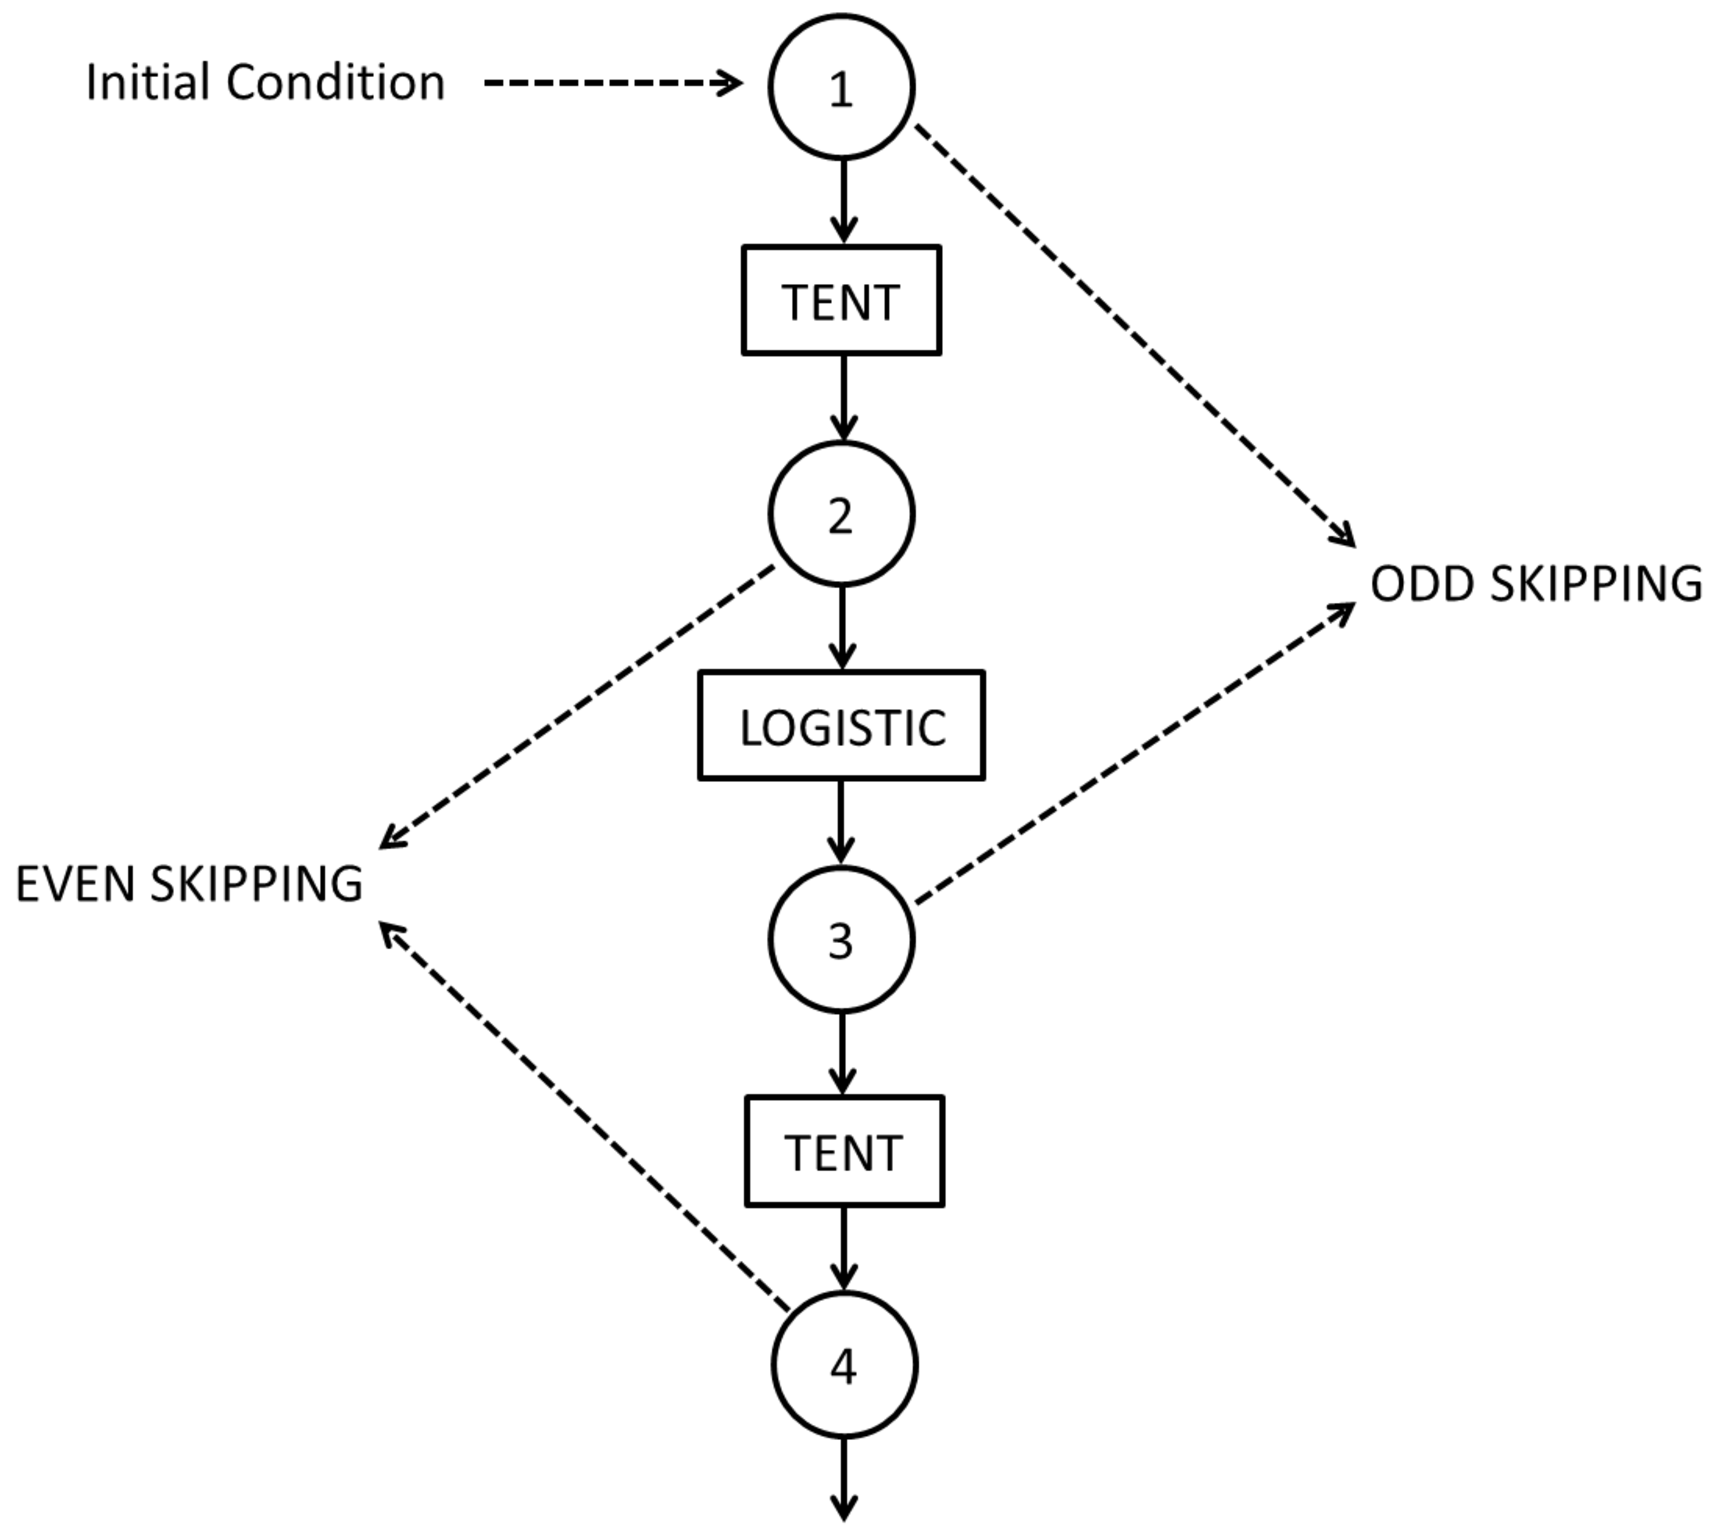
\includegraphics[height=0.4\textheight]{SwitchParImpar}
\caption{ZONA CH REHACER} \label{fig:plane zone}
\end{figure}
%%%%%%%%%%%%%%%%%%%%%%%%%%
%%%%%%%%%%%%%%%%%%%%%%%%%%% Fig.1
%
\begin{figure}
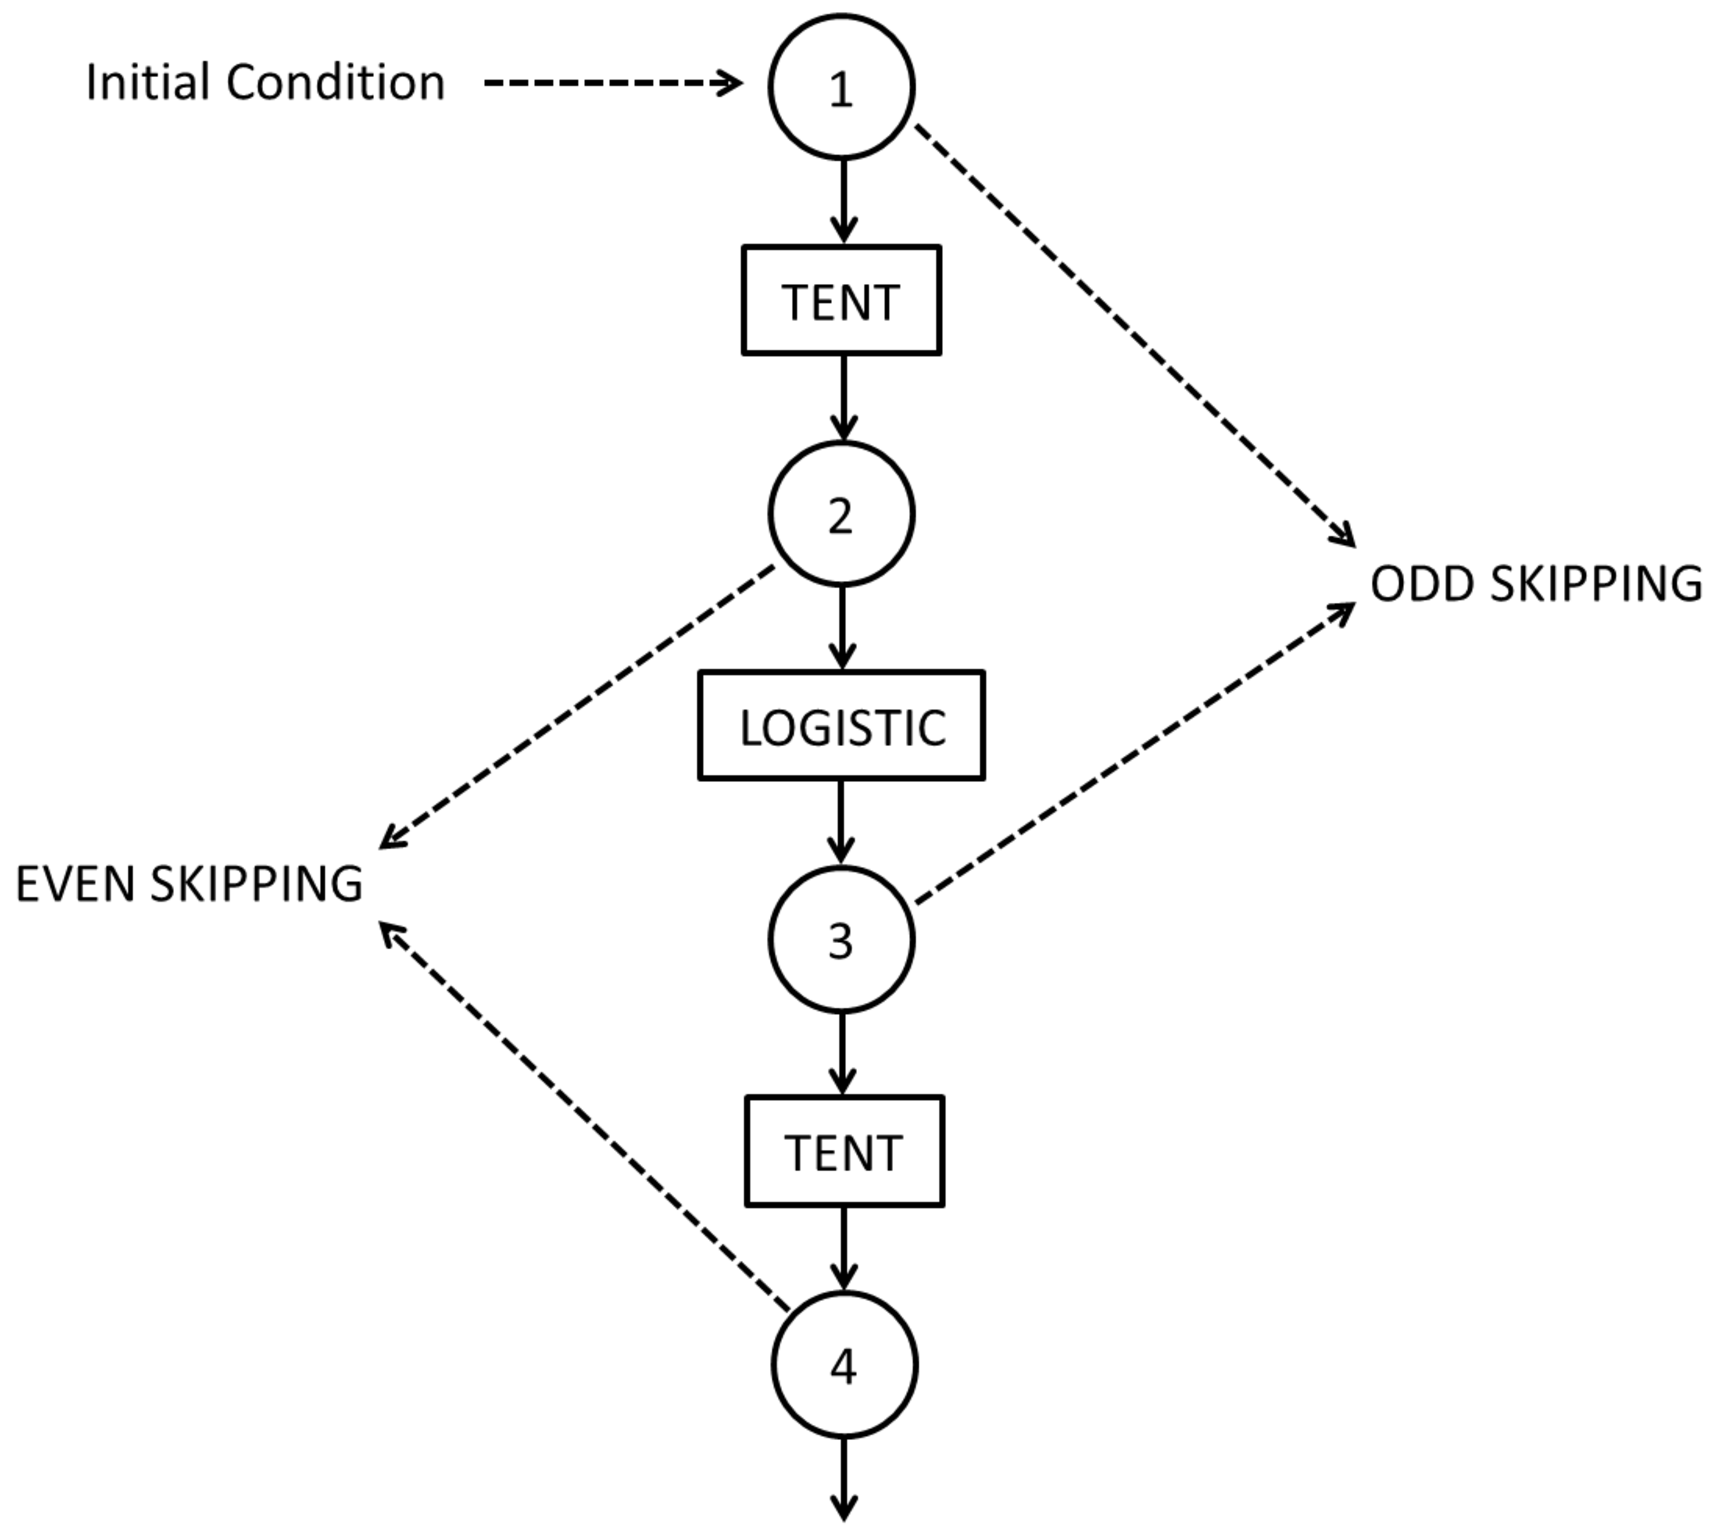
\includegraphics[height=0.4\textheight]{SwitchParImpar}
\caption{Sequential switching between Tent and Logistic maps. In the figure are also shown even and odd skipping strategies} \label{fig:seq}
\end{figure}
%%%%%%%%%%%%%%%%%%%%%%%%%%
%%%%%%%%%%%%%%%%%%%%%%%%%%% Fig.2
\begin{figure}
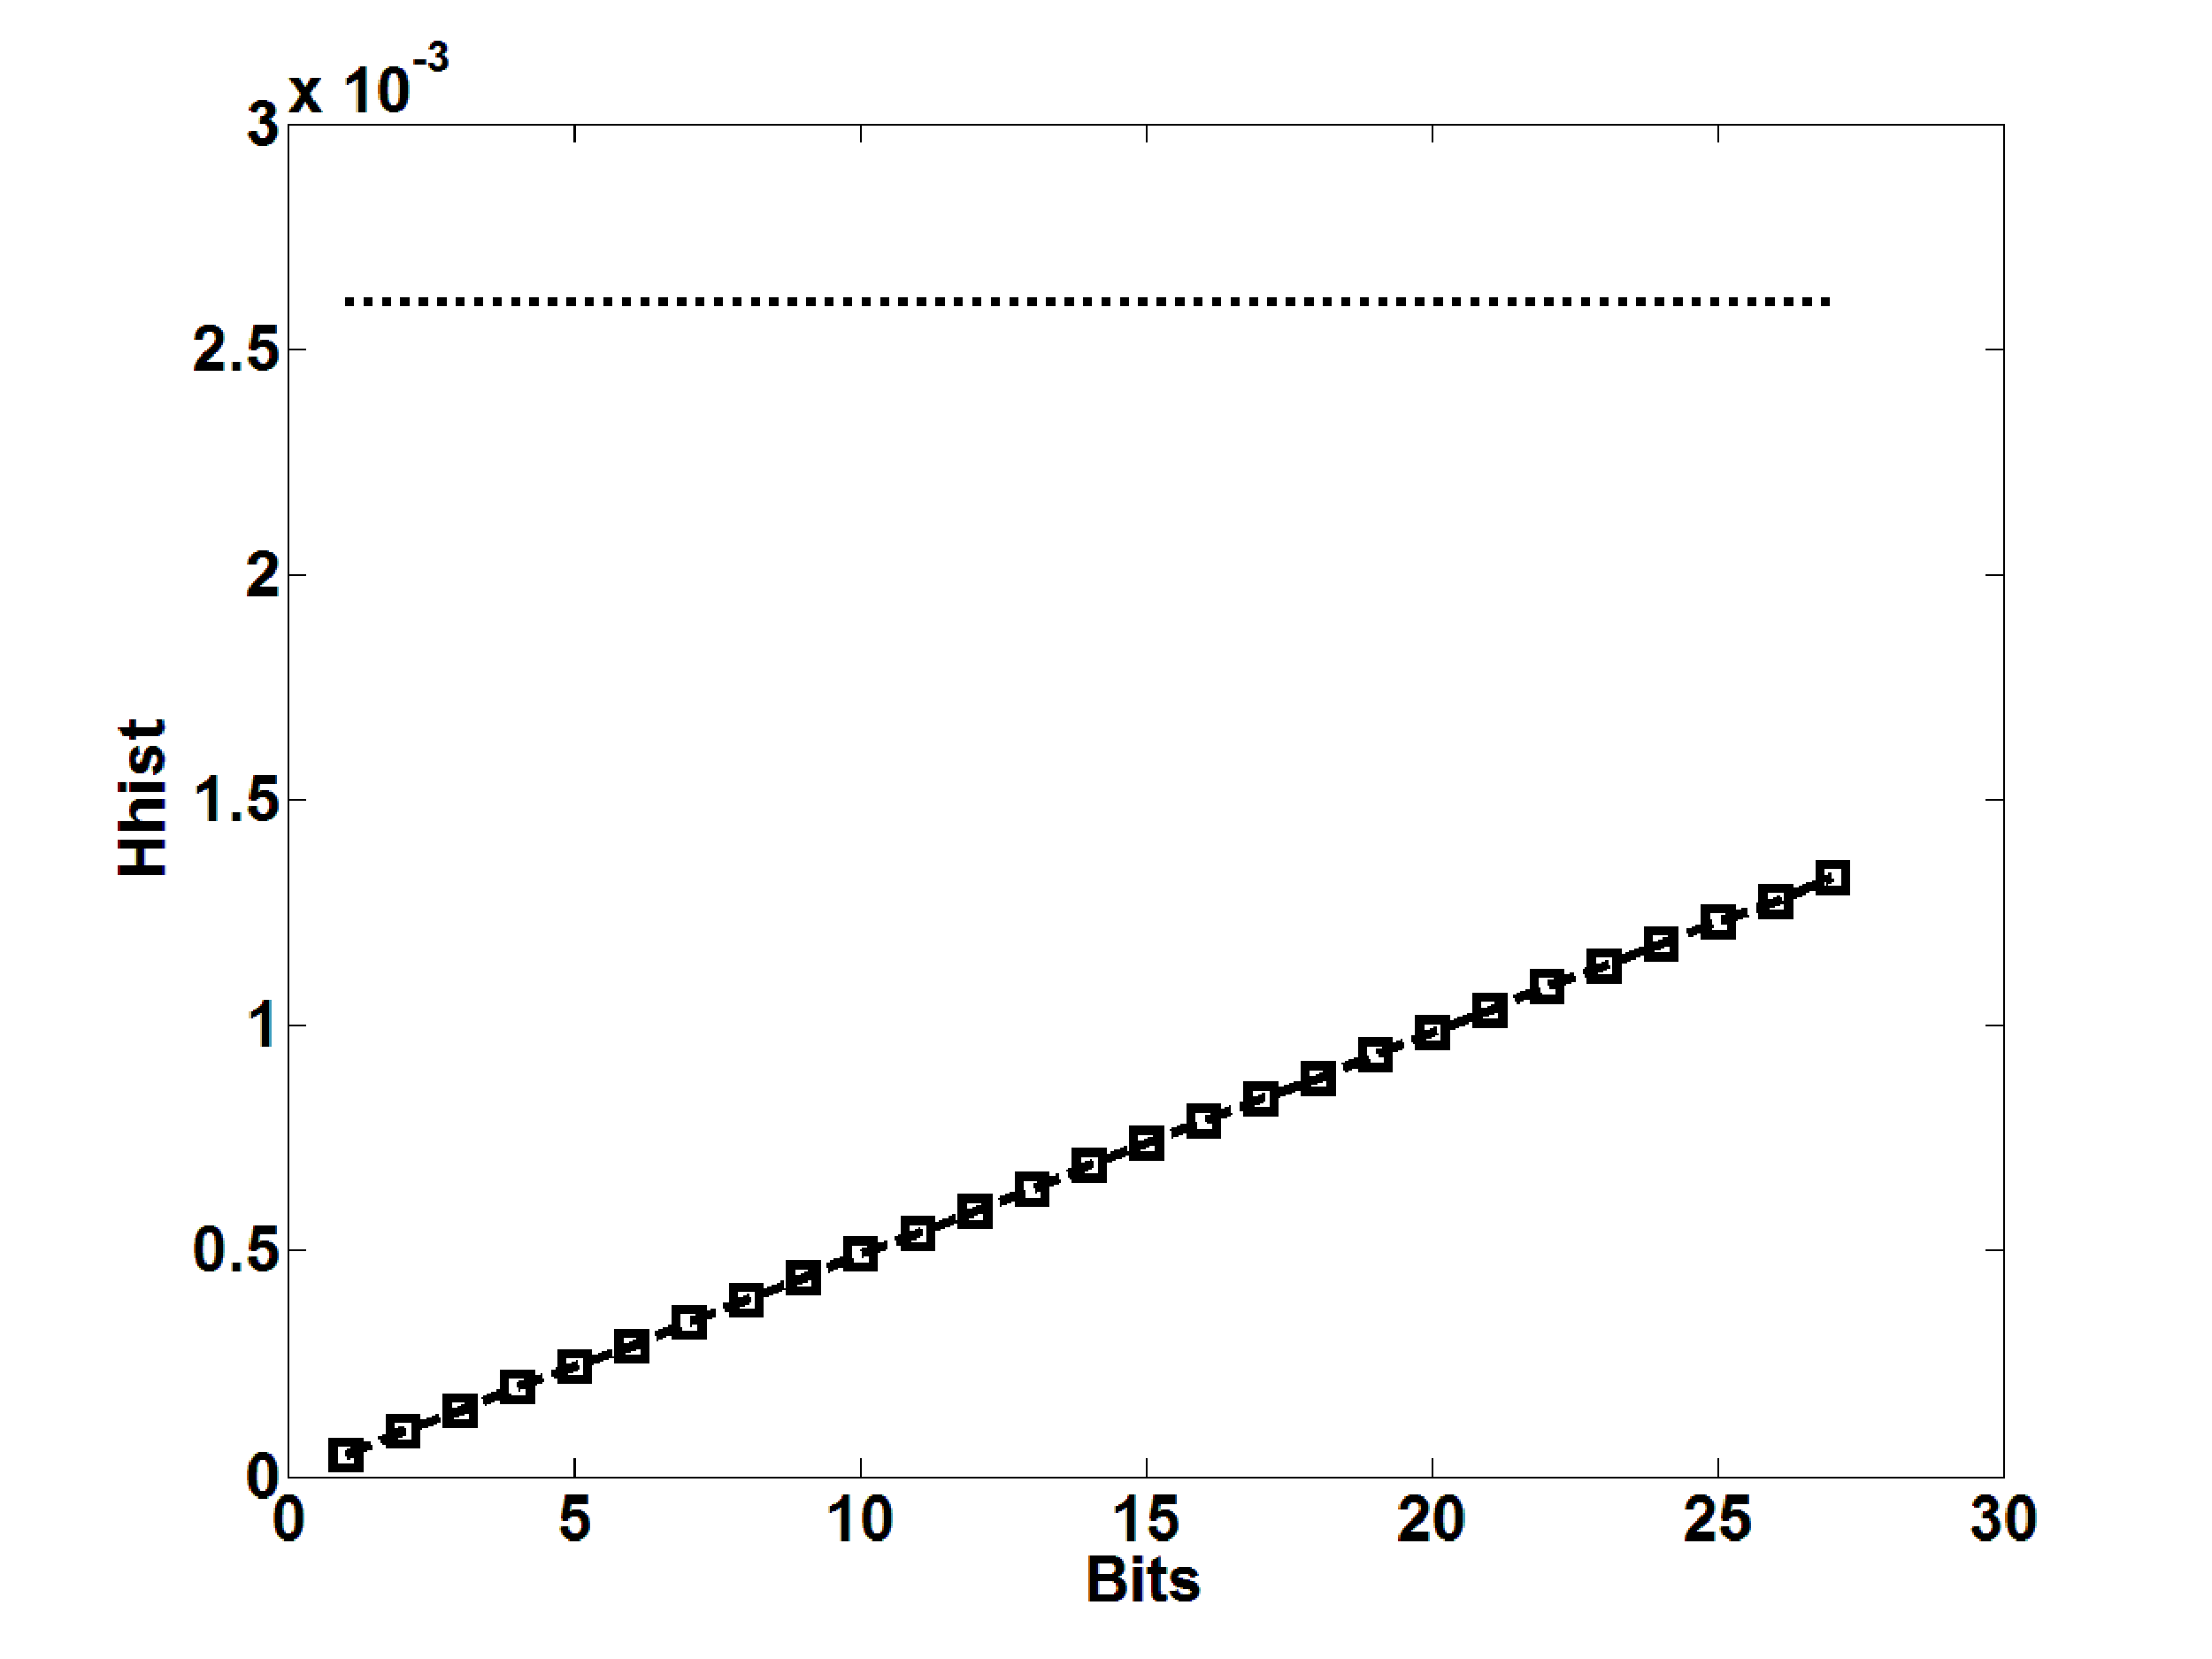
\includegraphics[width=0.3\textwidth]{Hhist_tentB10}
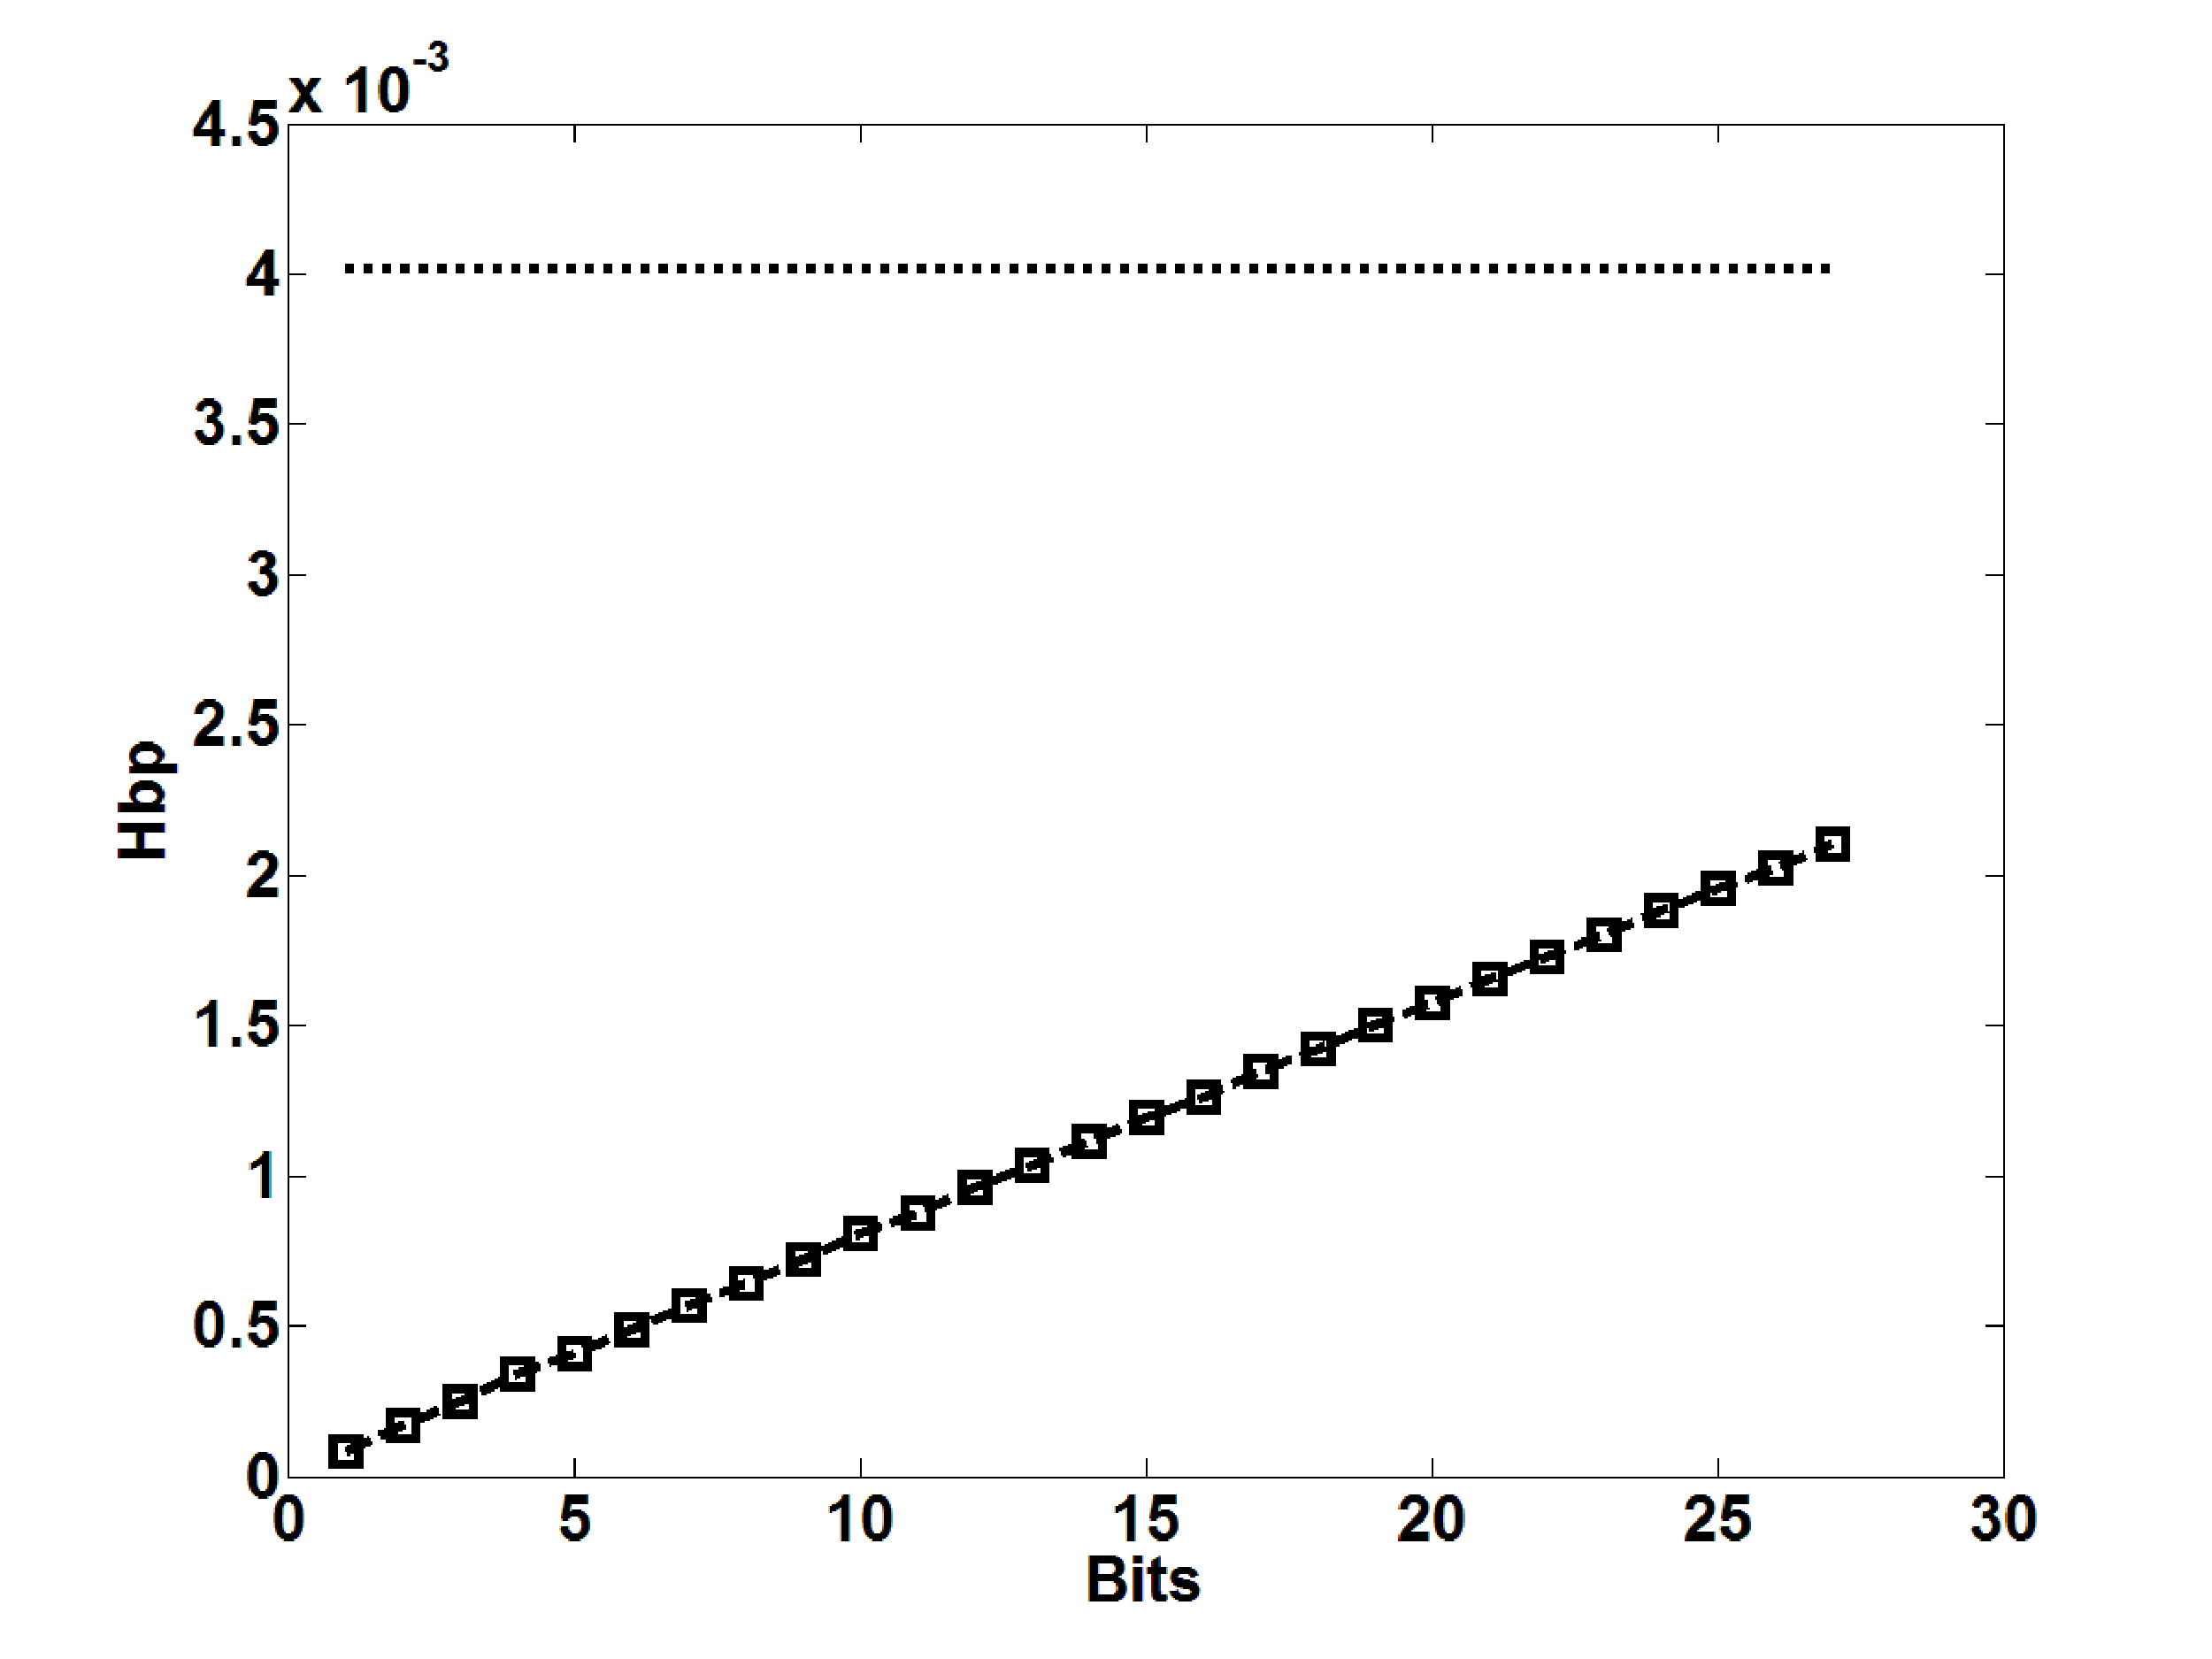
\includegraphics[width=0.3\textwidth]{Hbp_tentB10}
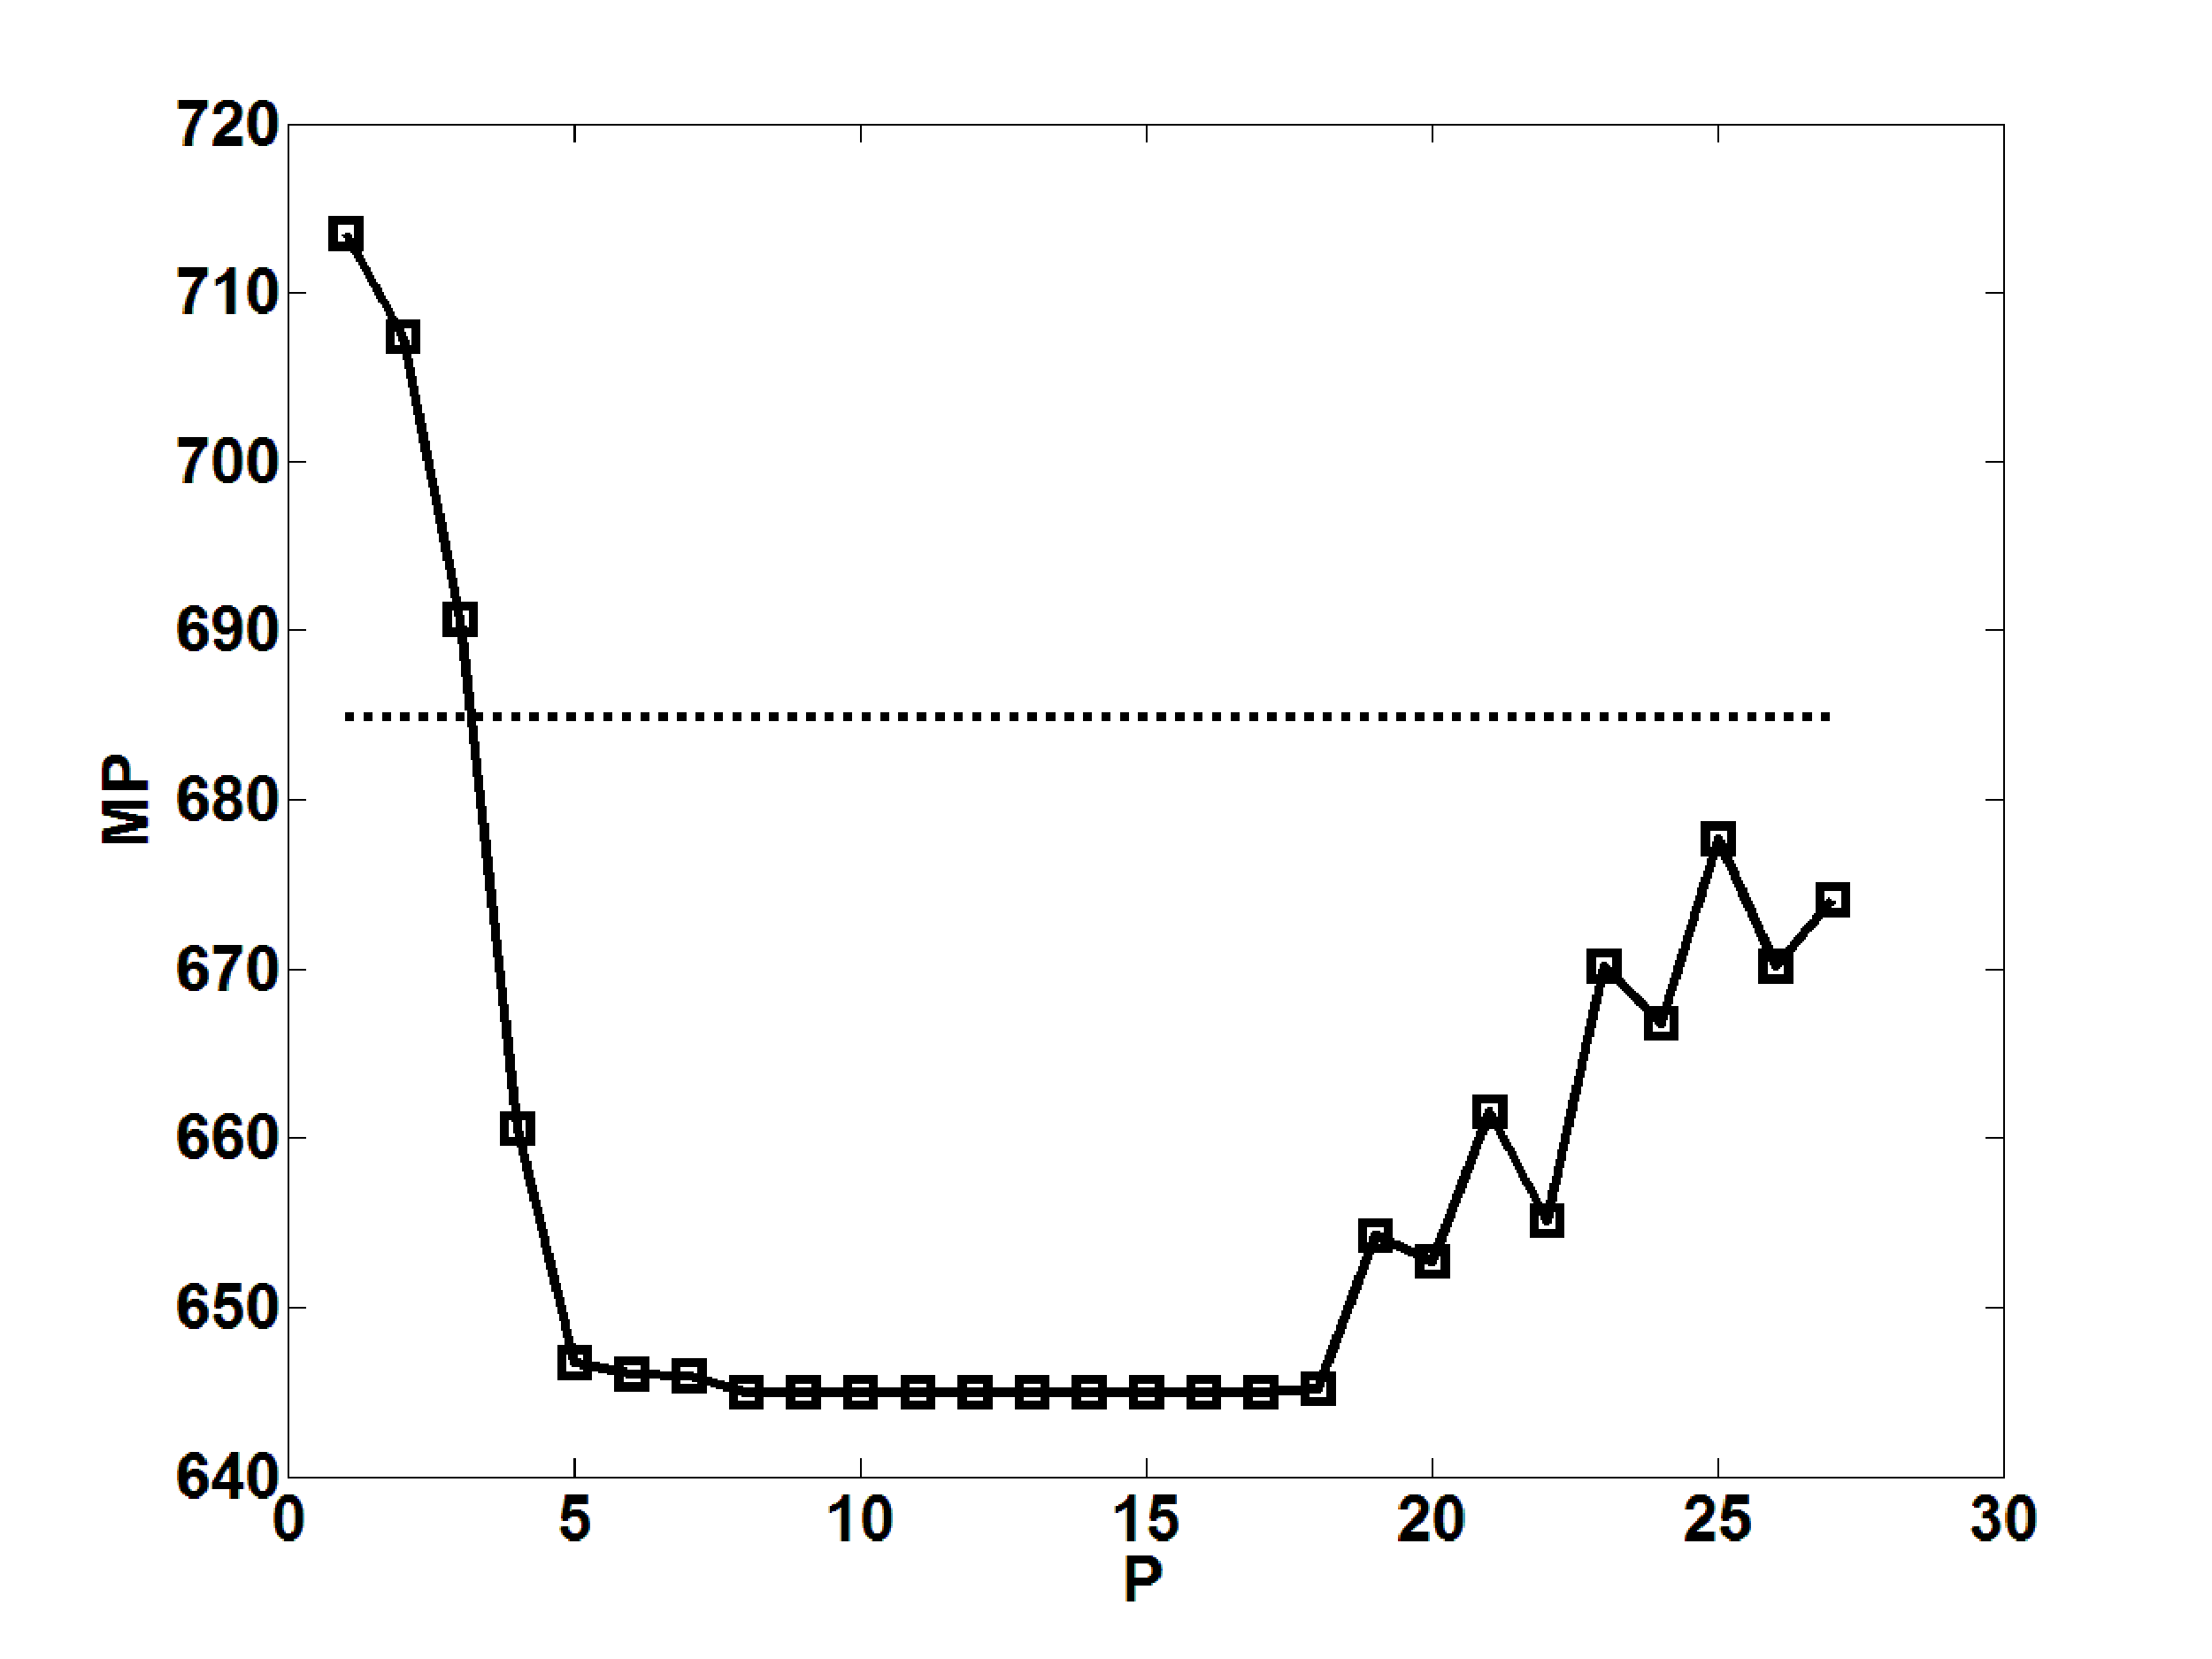
\includegraphics[width=0.3\textwidth]{Miss_tentB10}
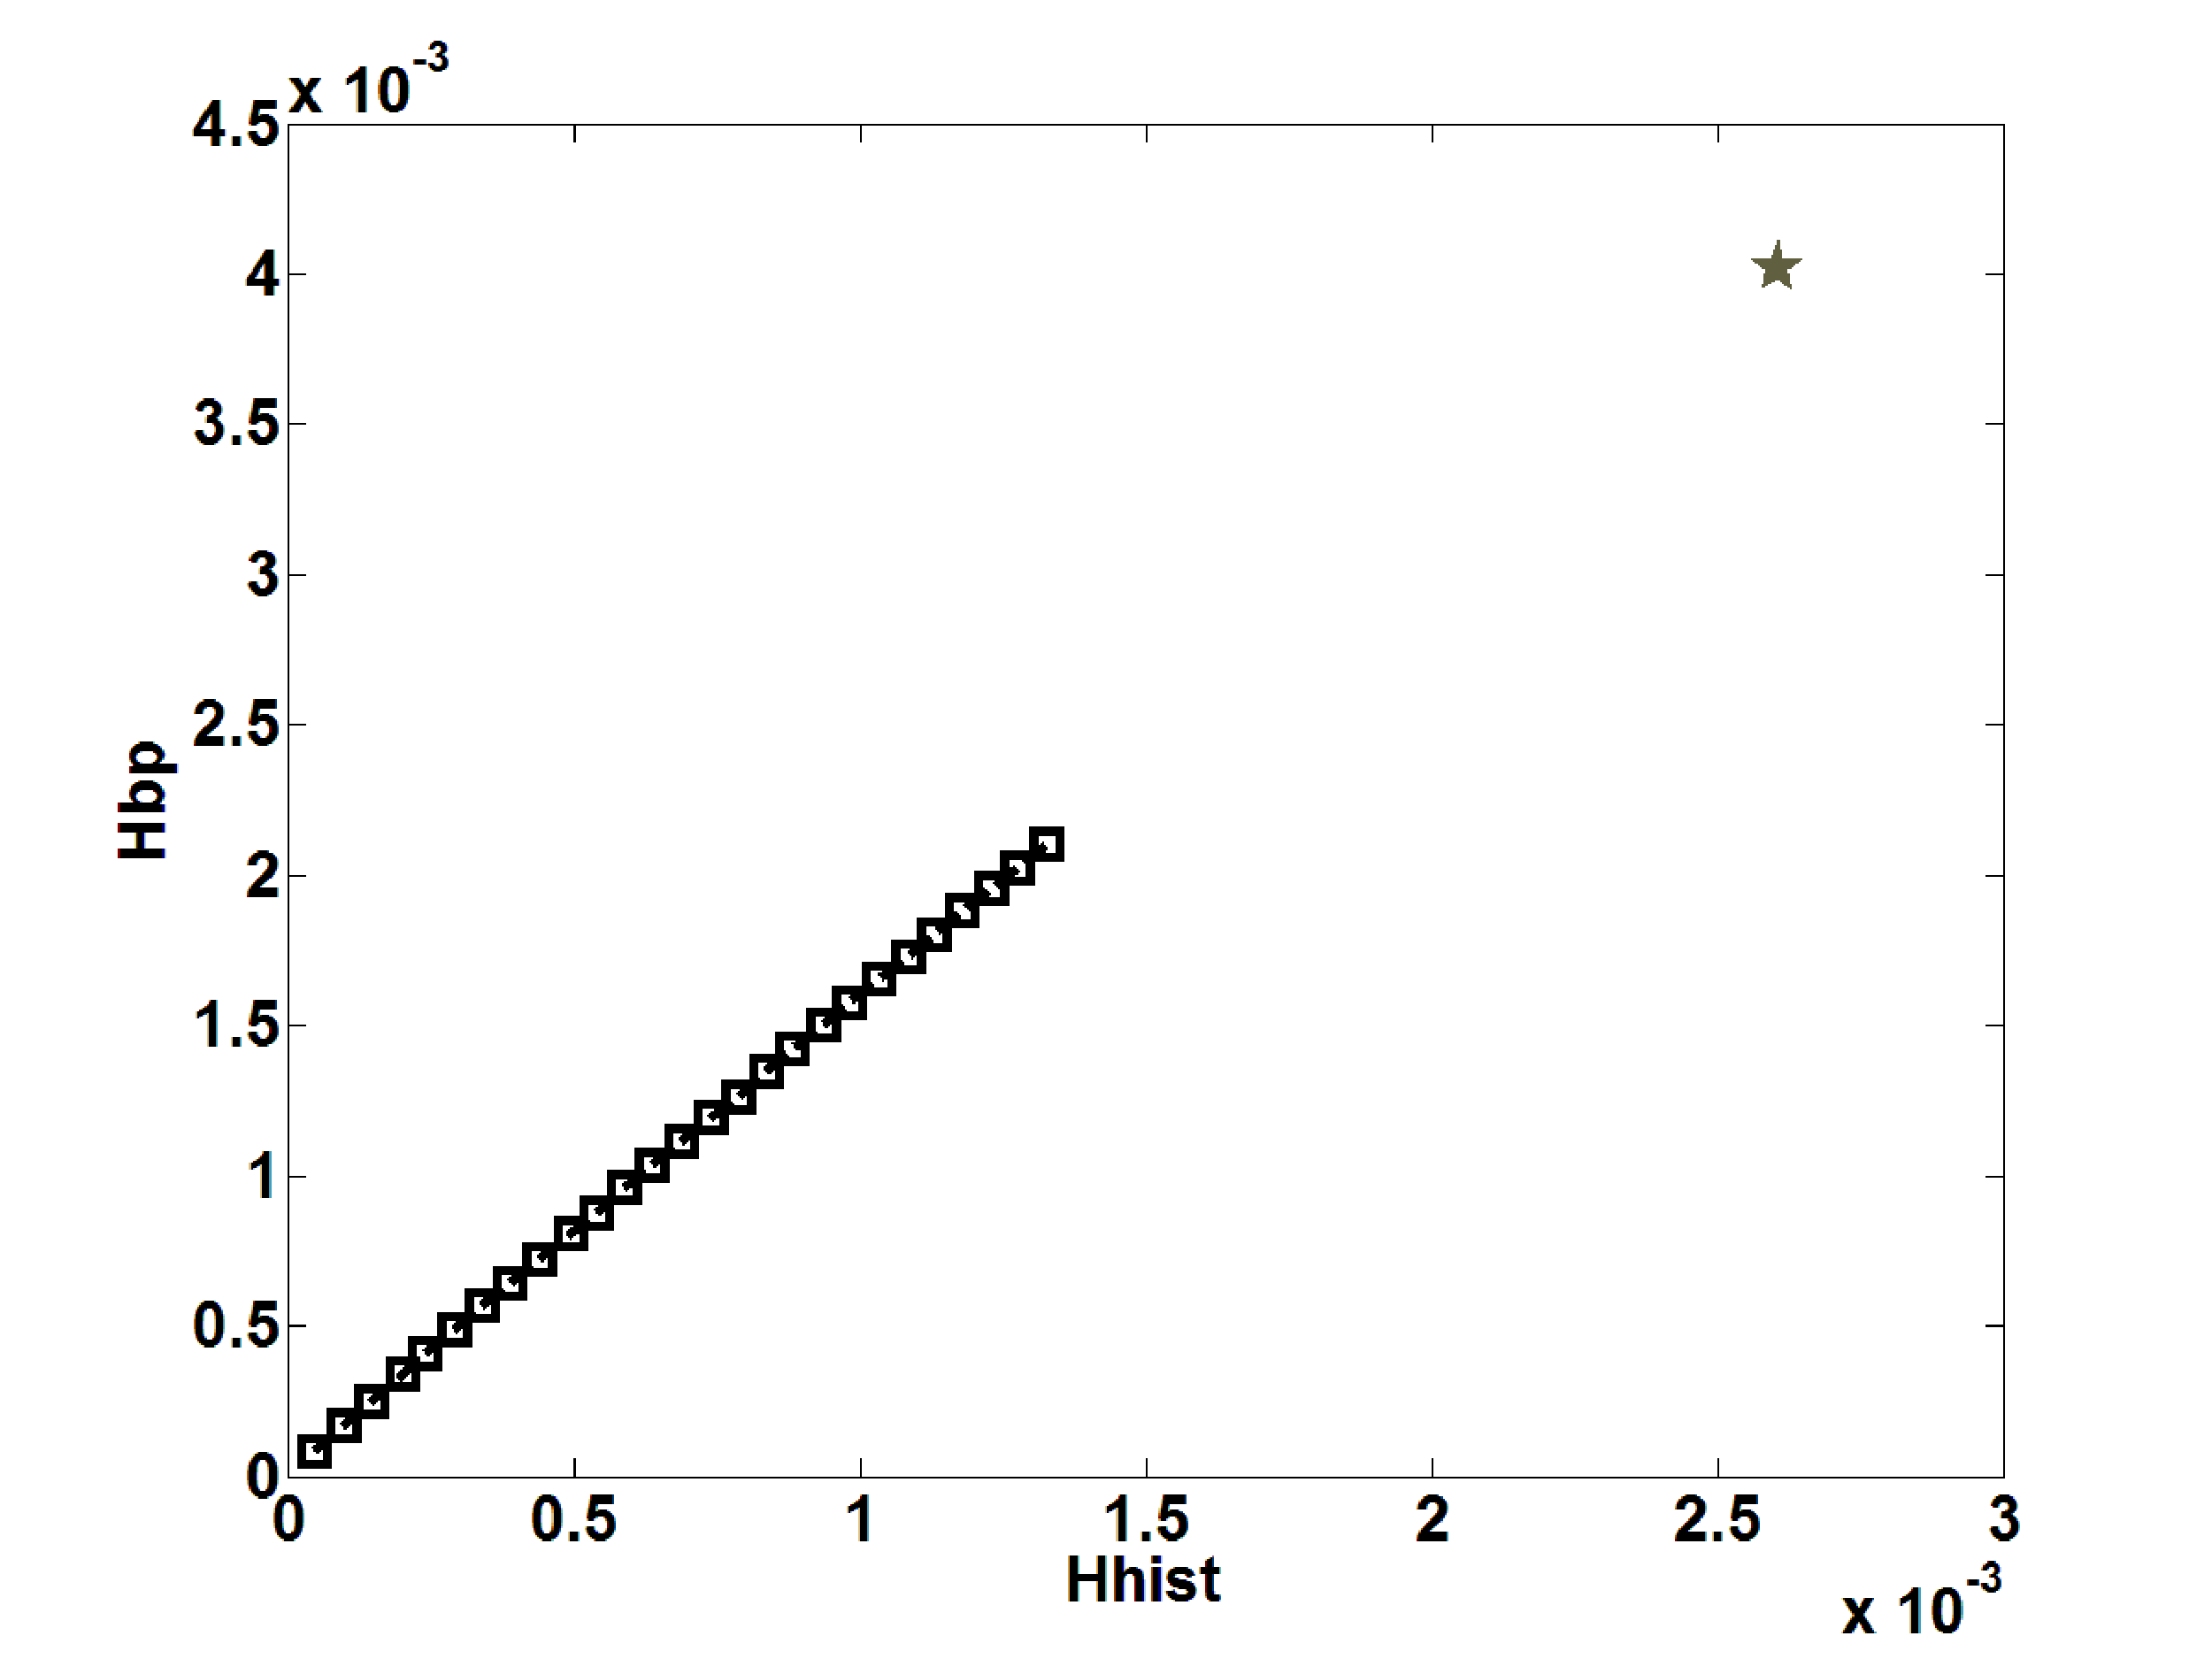
\includegraphics[width=0.3\textwidth]{HhistHbp_tentB10}
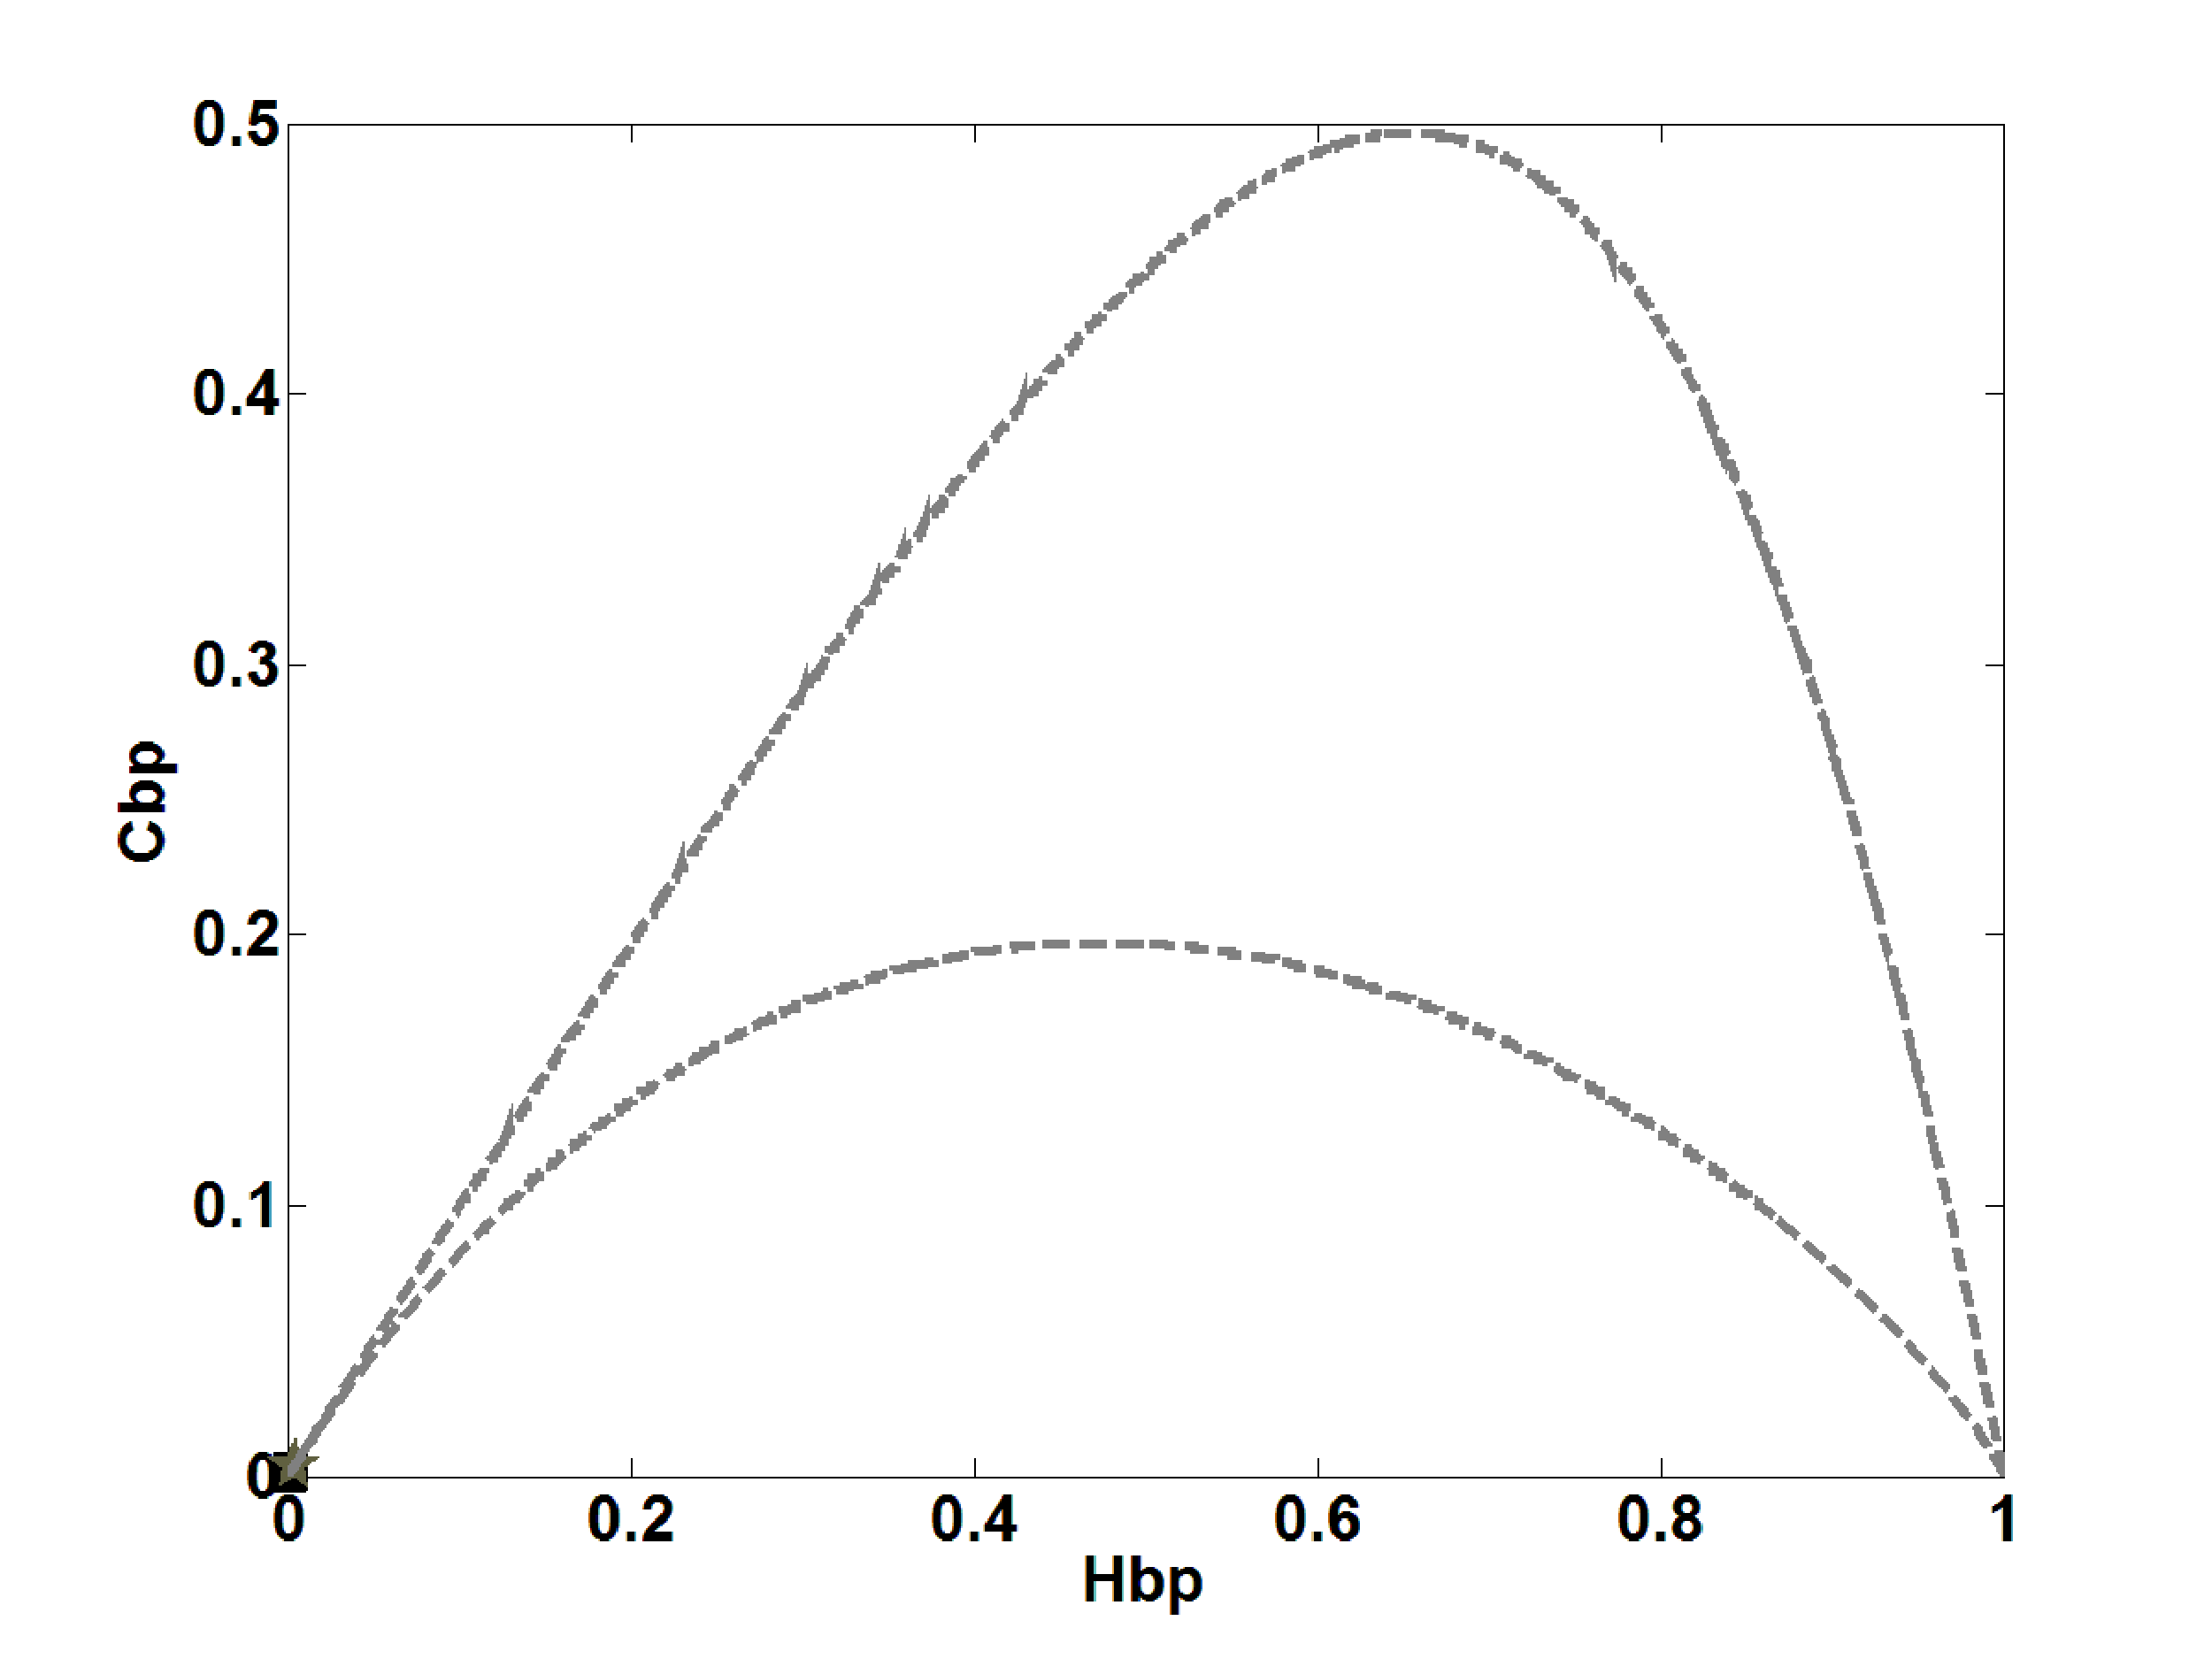
\includegraphics[width=0.3\textwidth]{HbpCbp_tentB10}
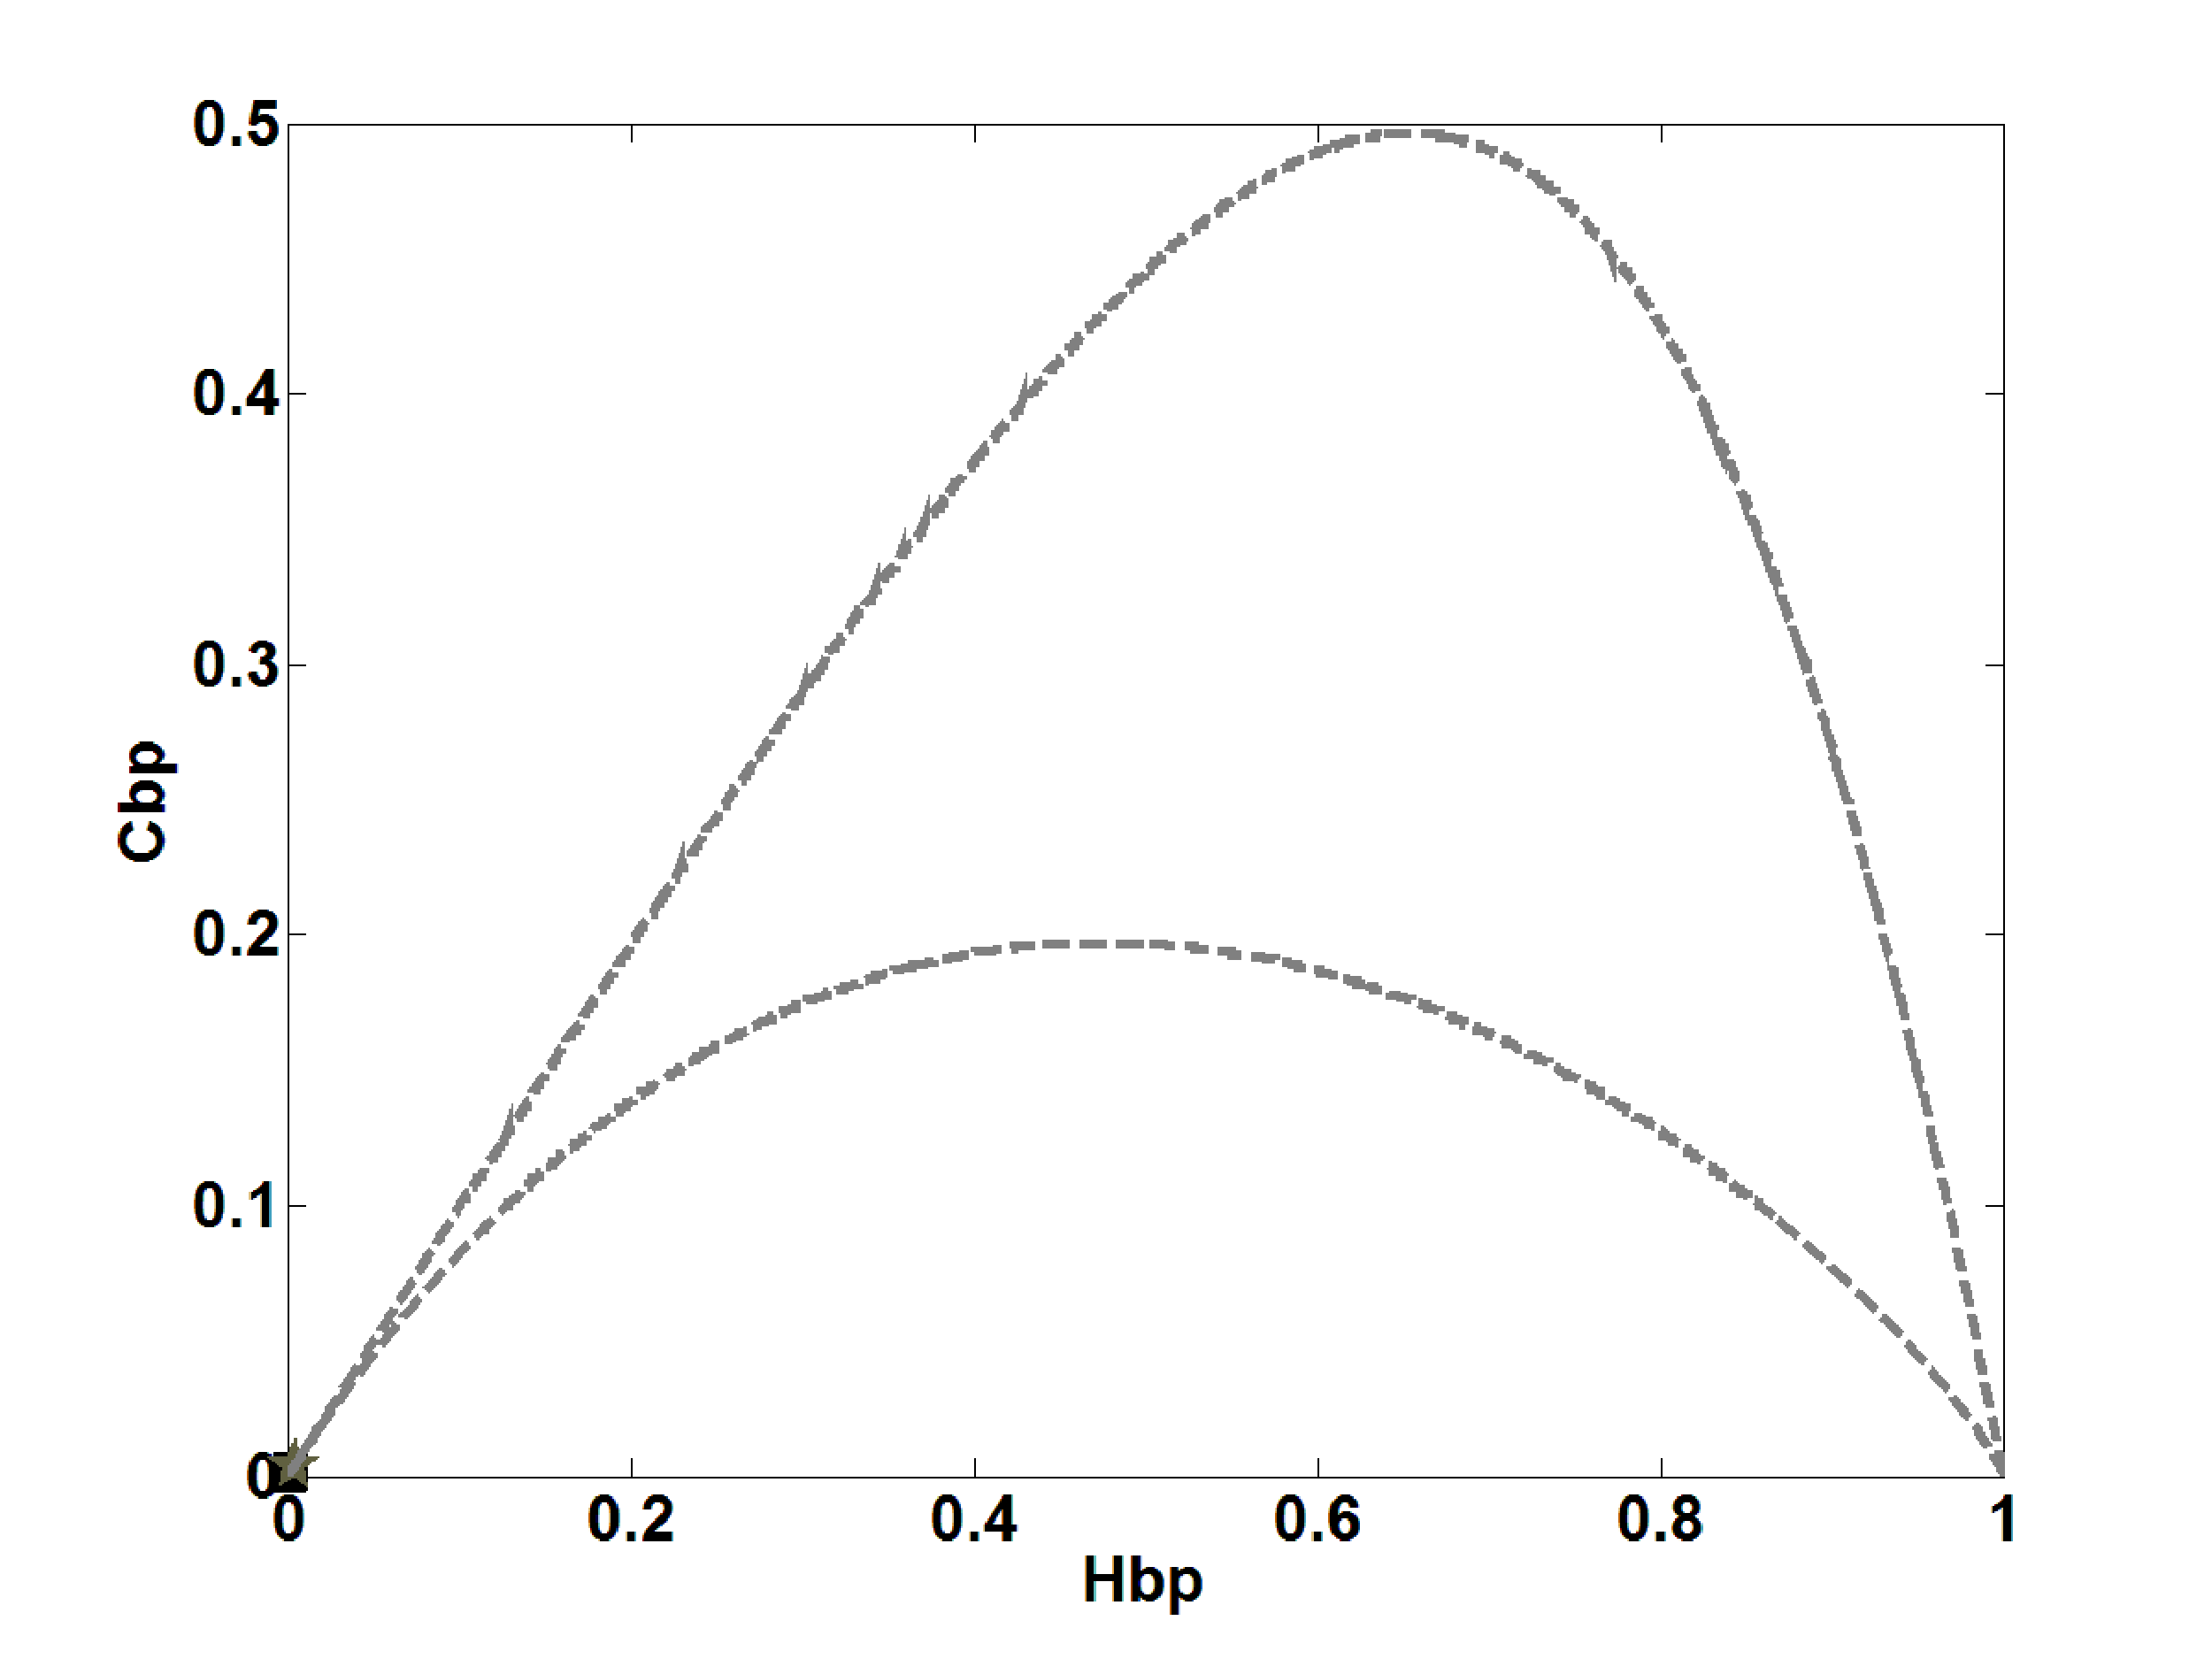
\includegraphics[width=0.3\textwidth]{HbpCbp_tentB2}
\caption{Statistical properties of the Tent map using different numerical representations. Figures (a) to(e) correspond to decimal representation: (a) $H_{hist}$ vs $P$ (b) $H_{BP}$ vs $P$ (c) Number of missing ordering patterns $MP$ vs $P$. In Figures (a) to (c) dashed line correspond to floating point numbers. (d) representation in the $H_{hist},H_{BP}$ plane in the the decimal numerical system.  The star represents the state for floating points numbers. (e) representation in the $H_{BP},C_{BP}$ plane.  The star represents the state for floating points numbers. (f) representation in the $H_{BP},C_{BP}$ plane for binary numerical system.  The star represents the state for floating points numbers. } \label{fig:tent}
\end{figure}

%%%%%%%%%%%%%%%%%%%%%%%%%%
%%%%%%%%%%%%%%%%%%%%%%%%%%% Fig.3
\begin{figure}
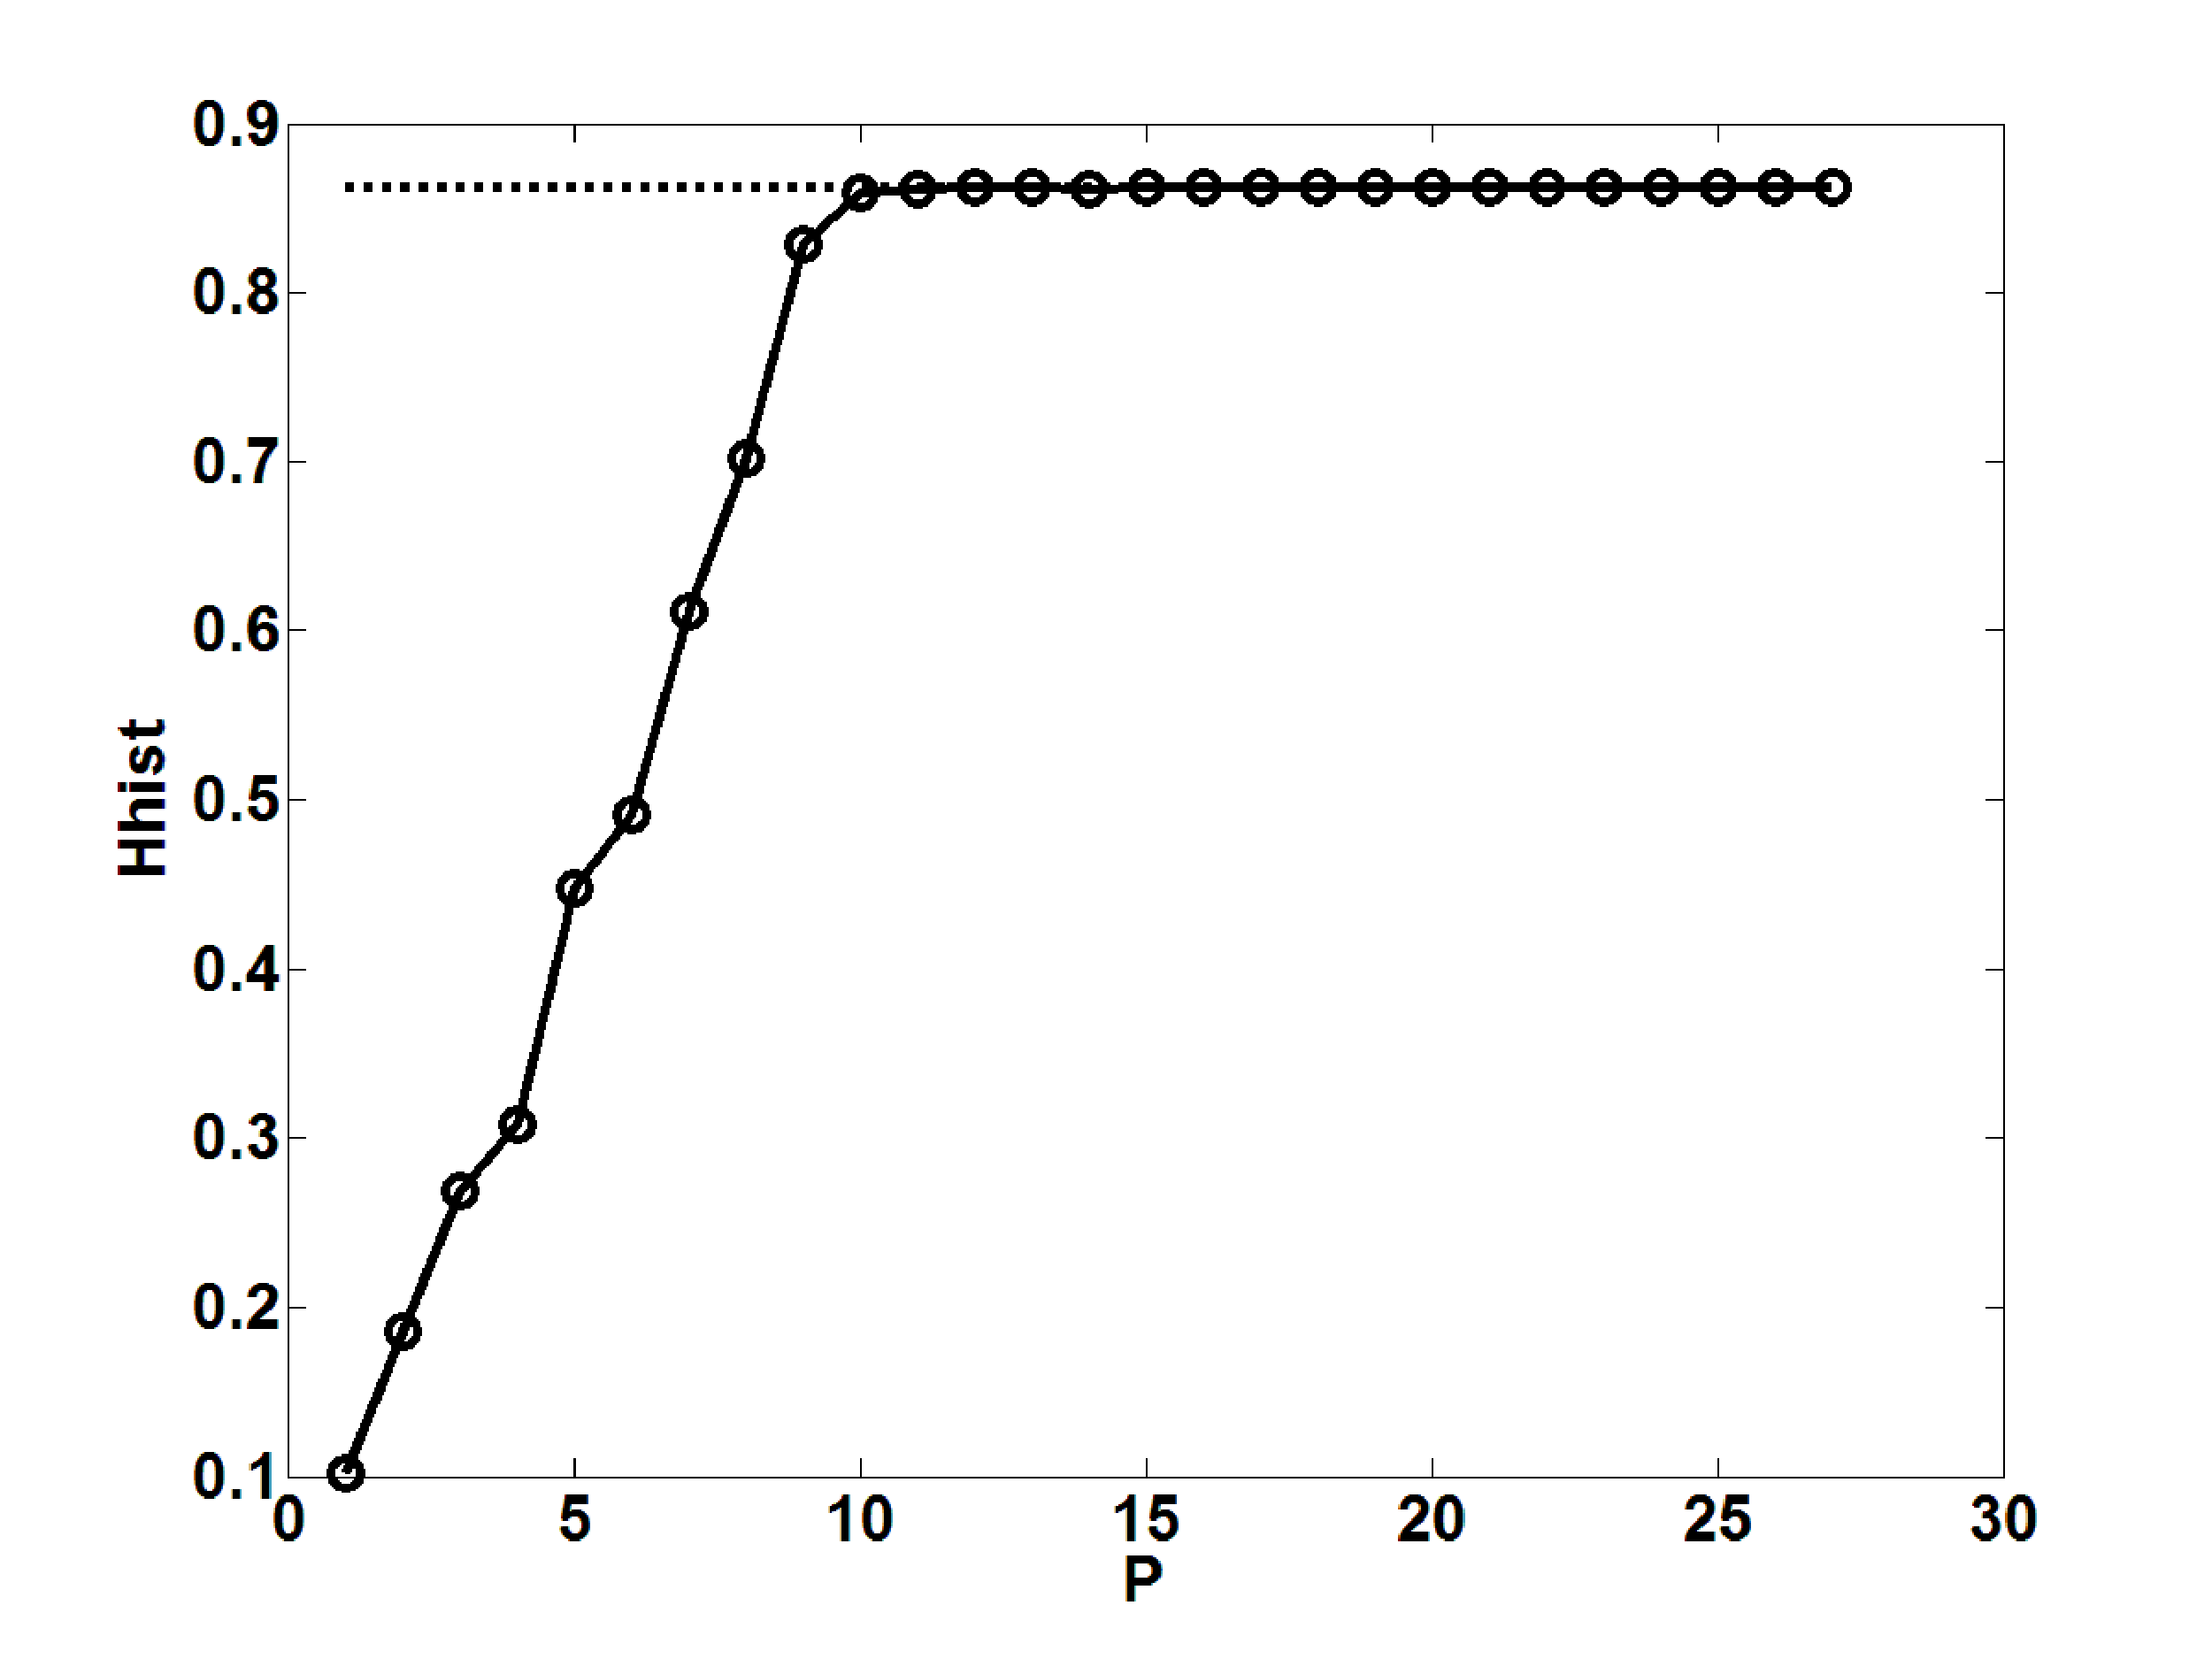
\includegraphics[width=0.3\textwidth]{Hhist_logisticoB10}
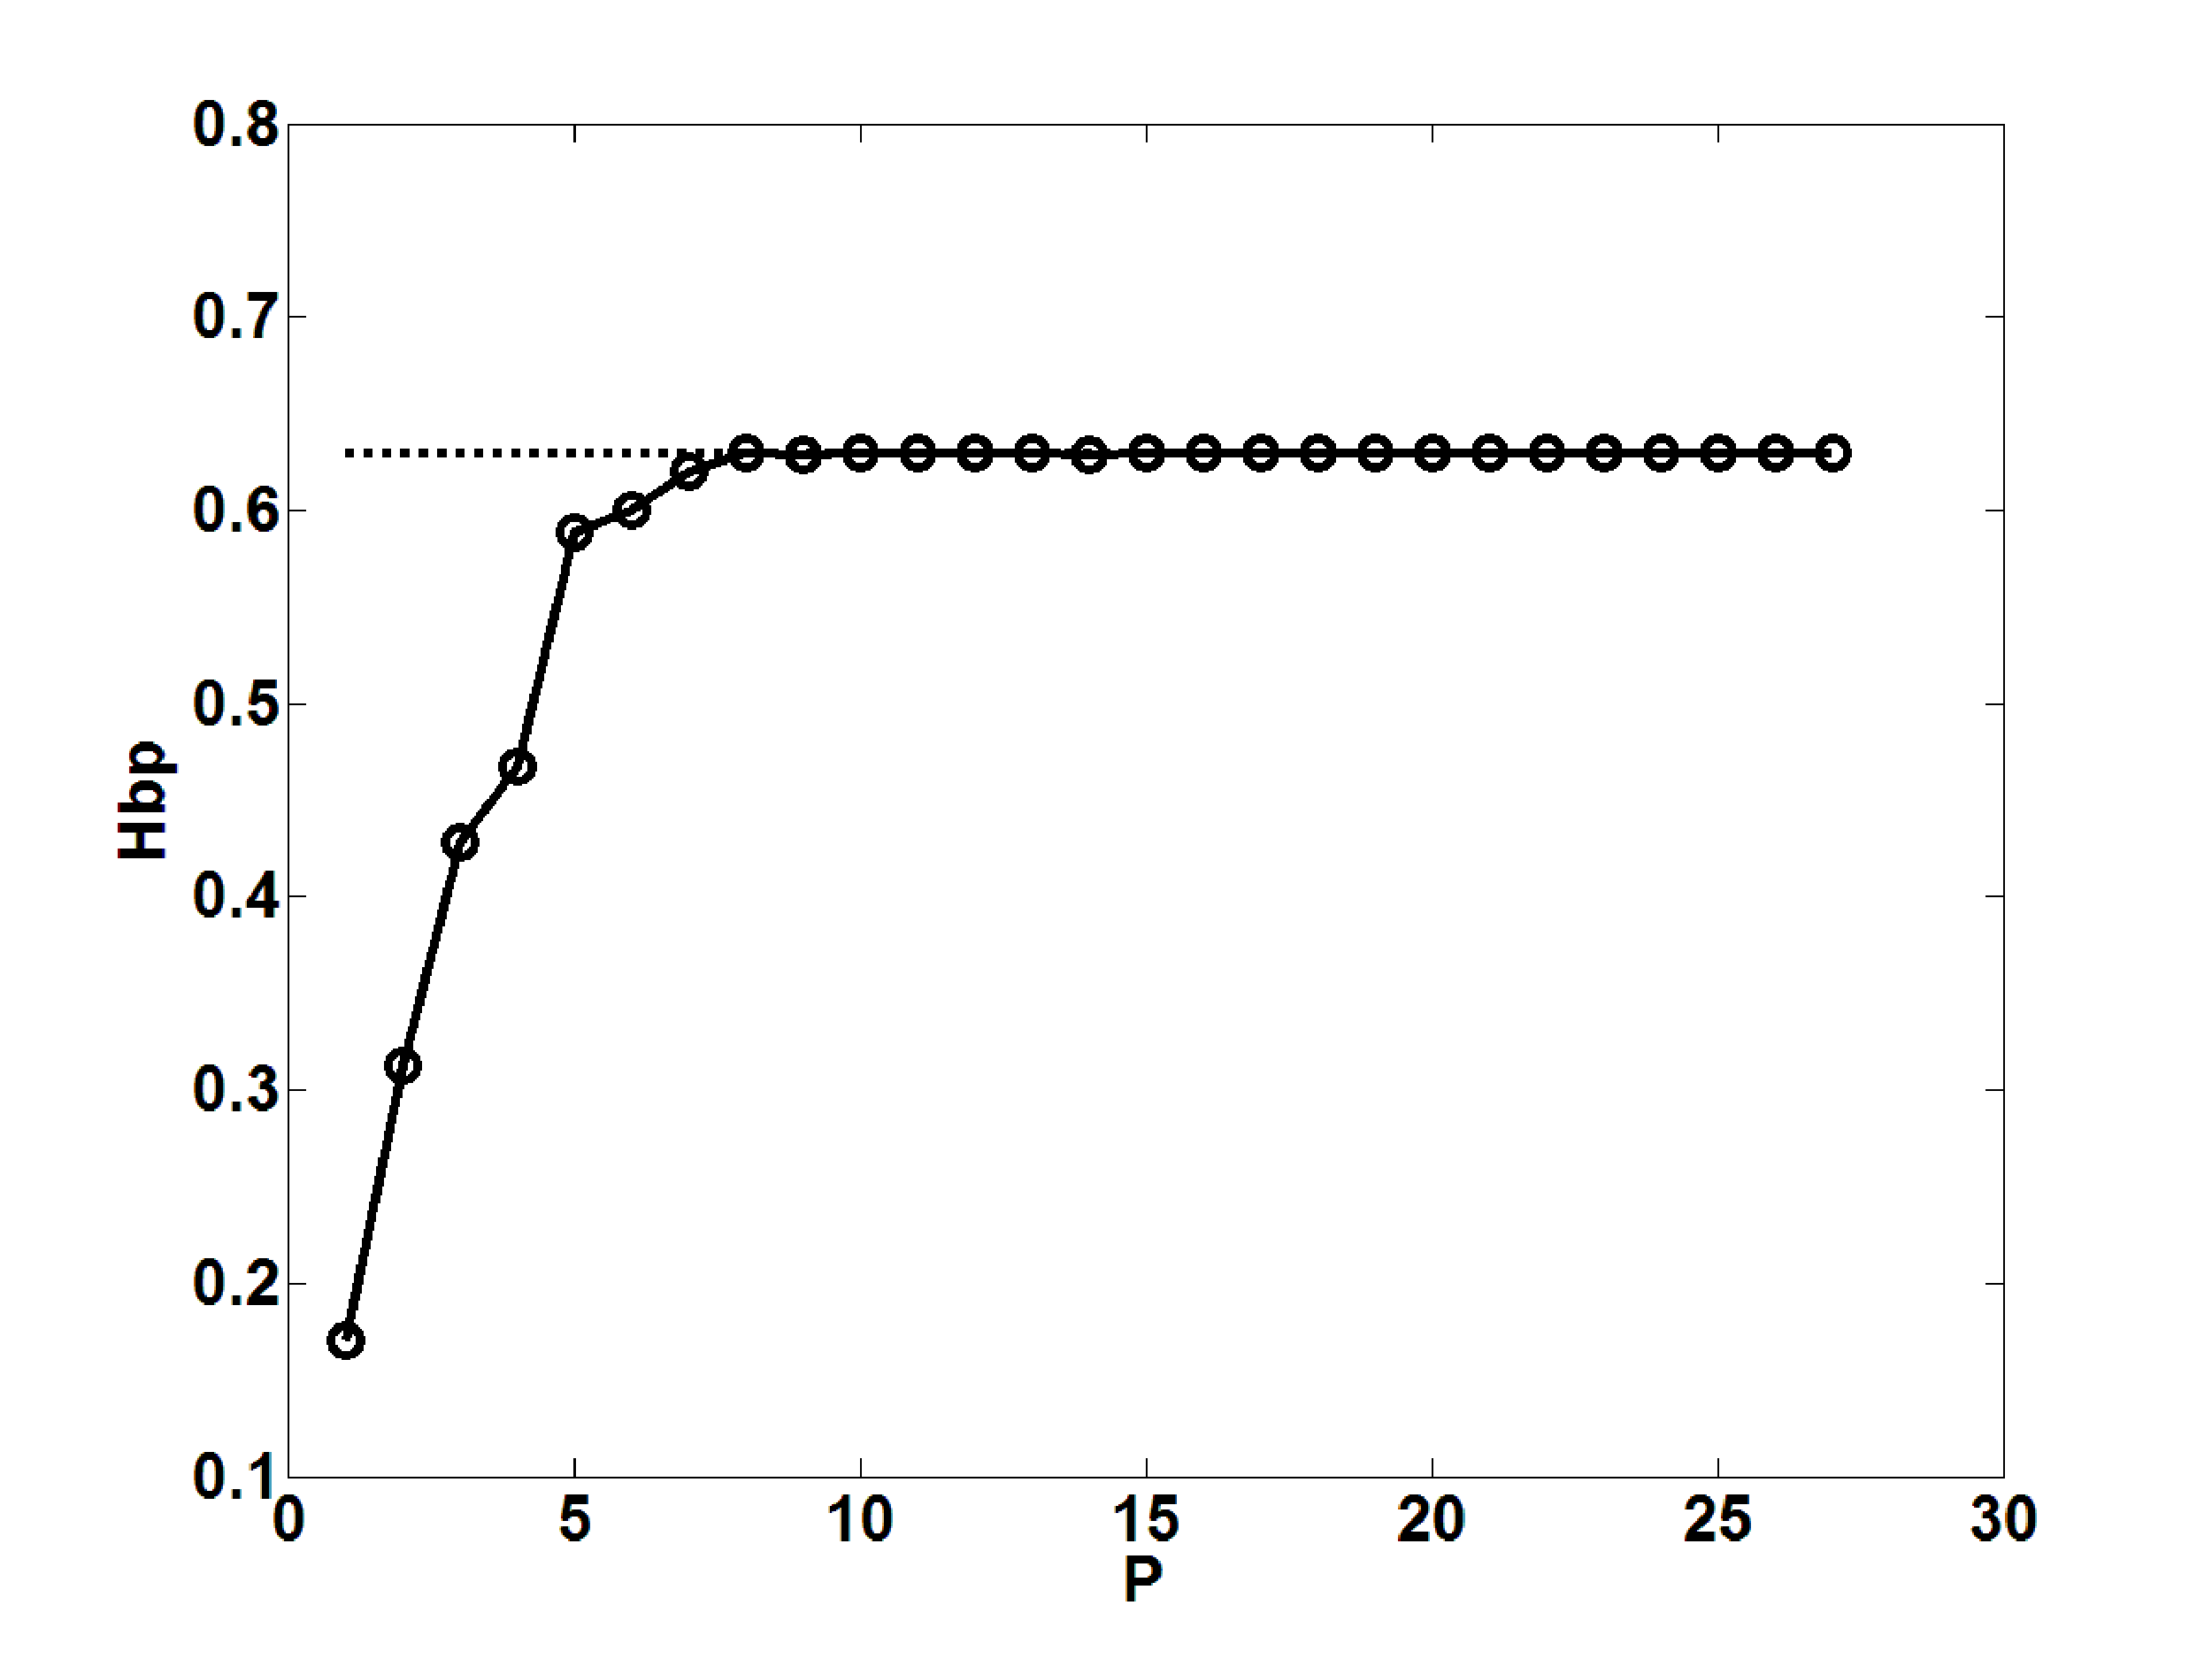
\includegraphics[width=0.3\textwidth]{Hbp_logisticoB10}
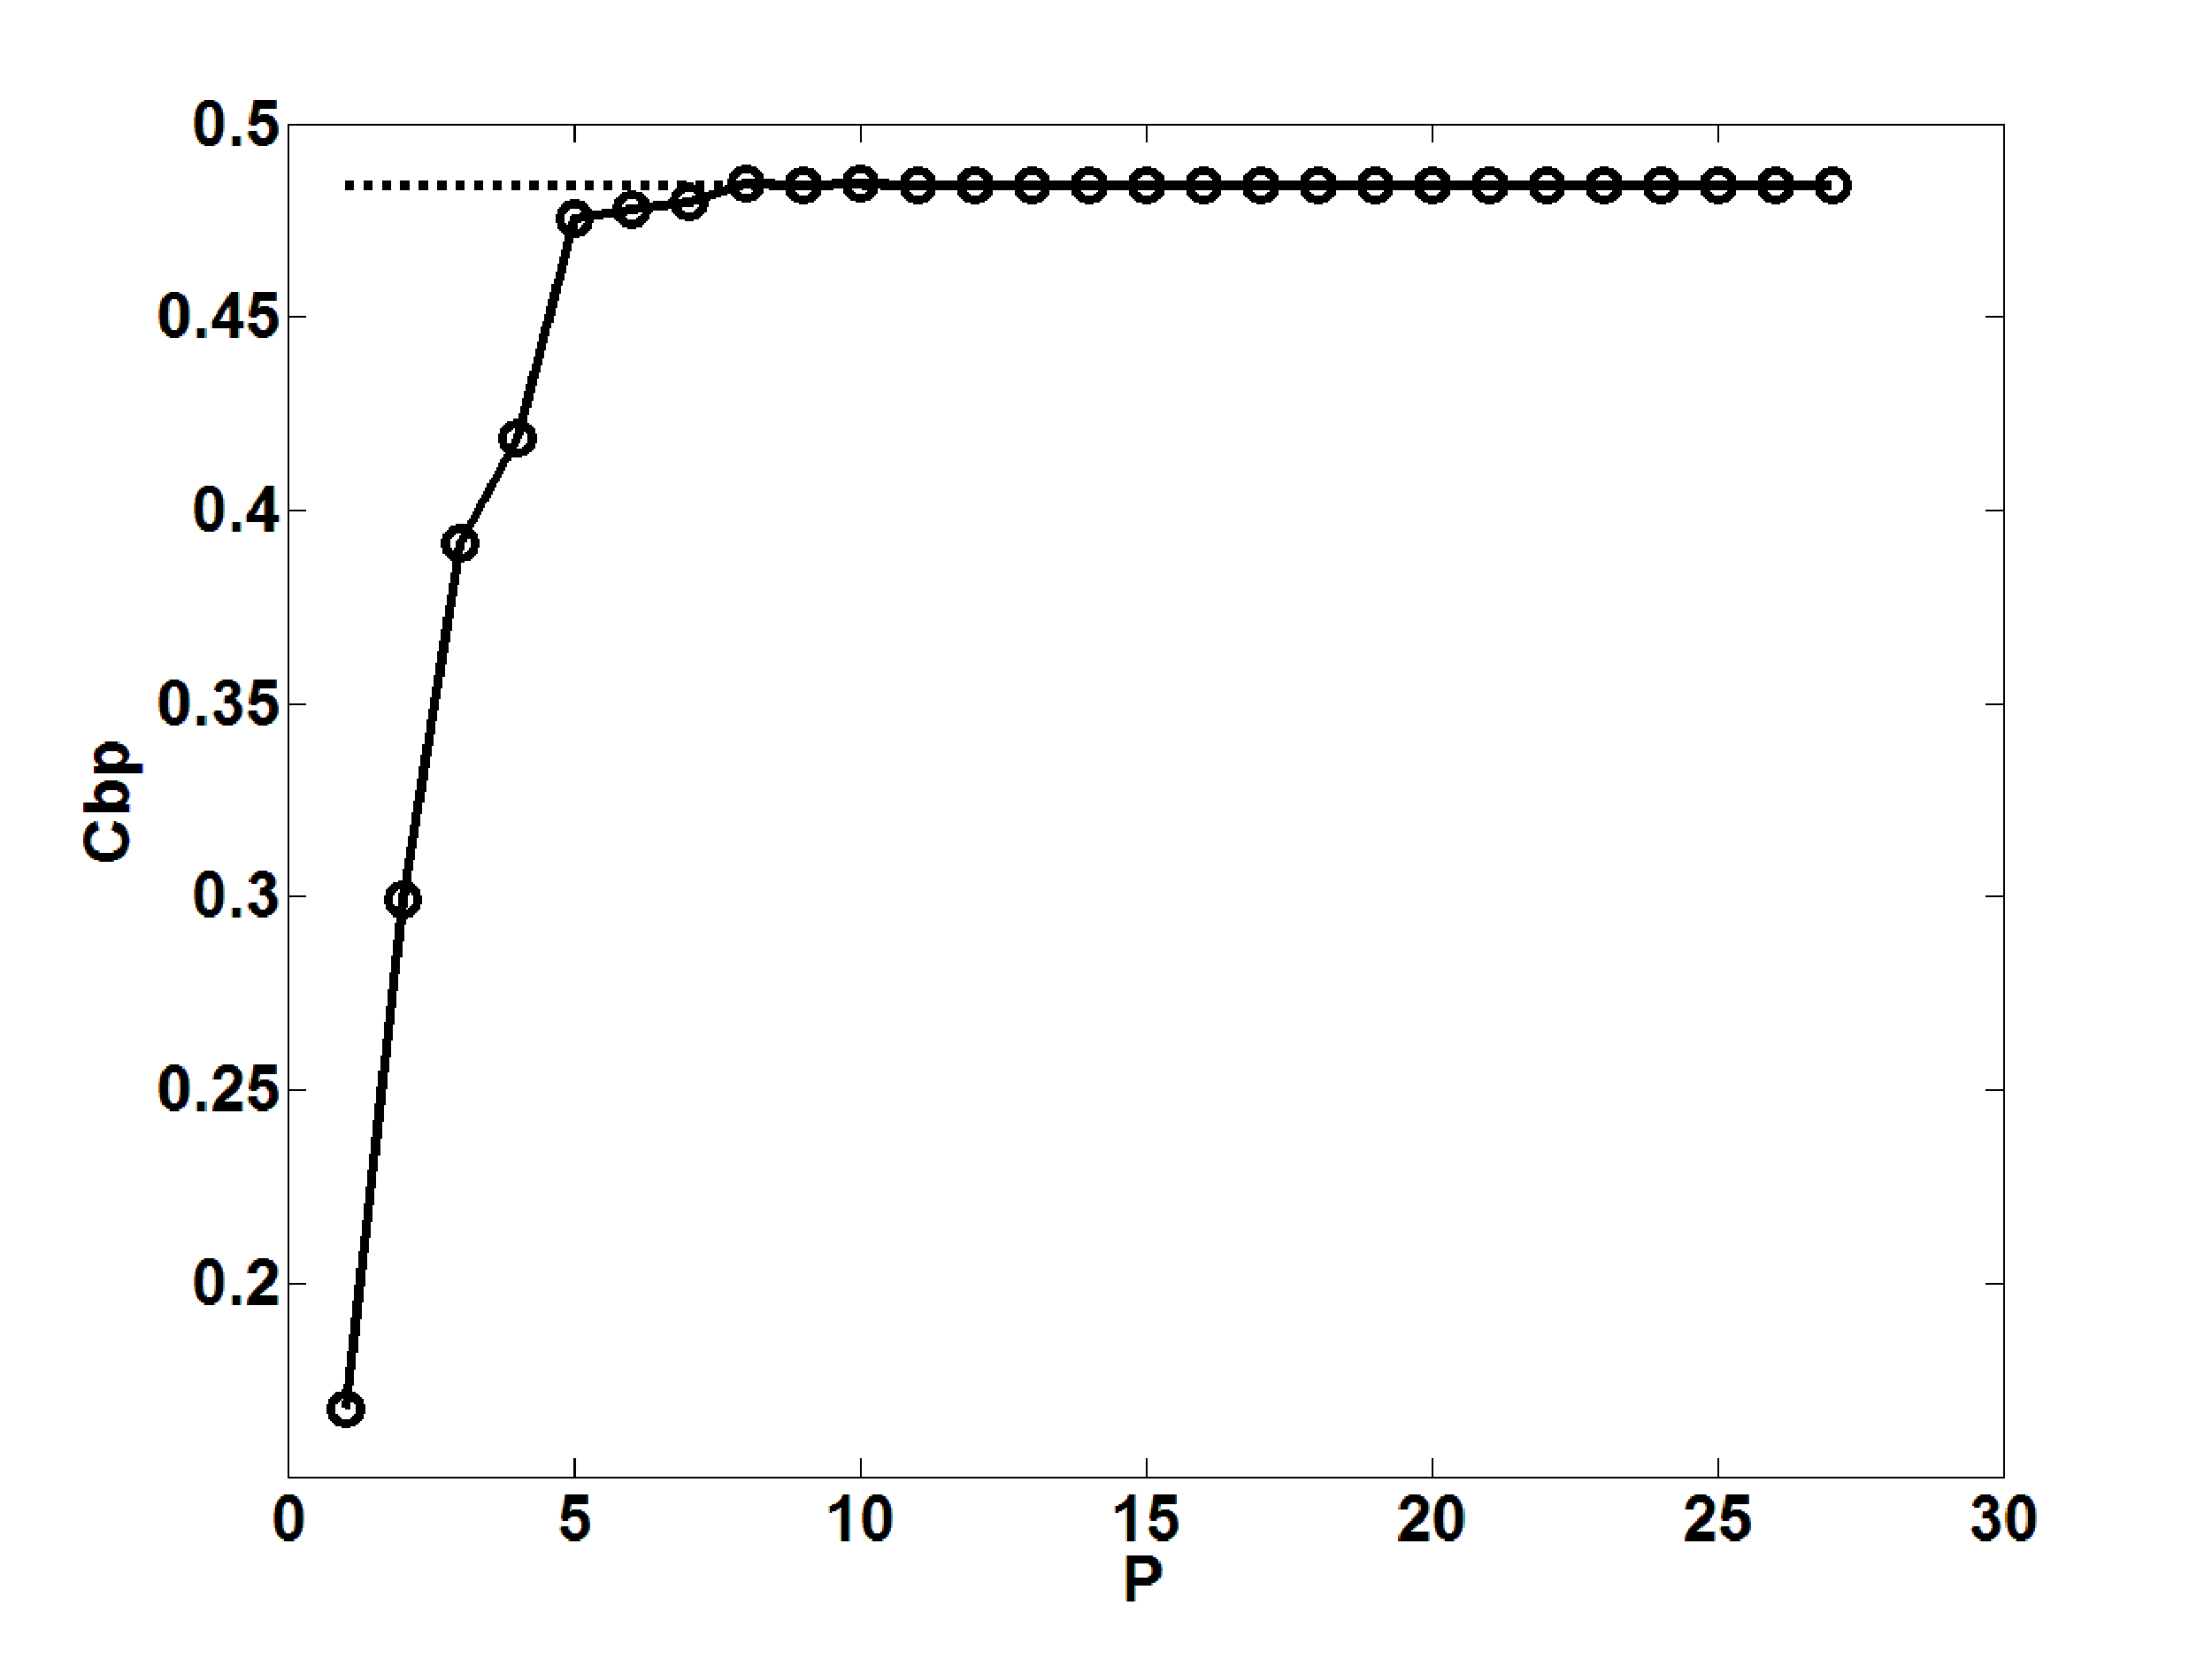
\includegraphics[width=0.3\textwidth]{Cbp_logisticoB10}
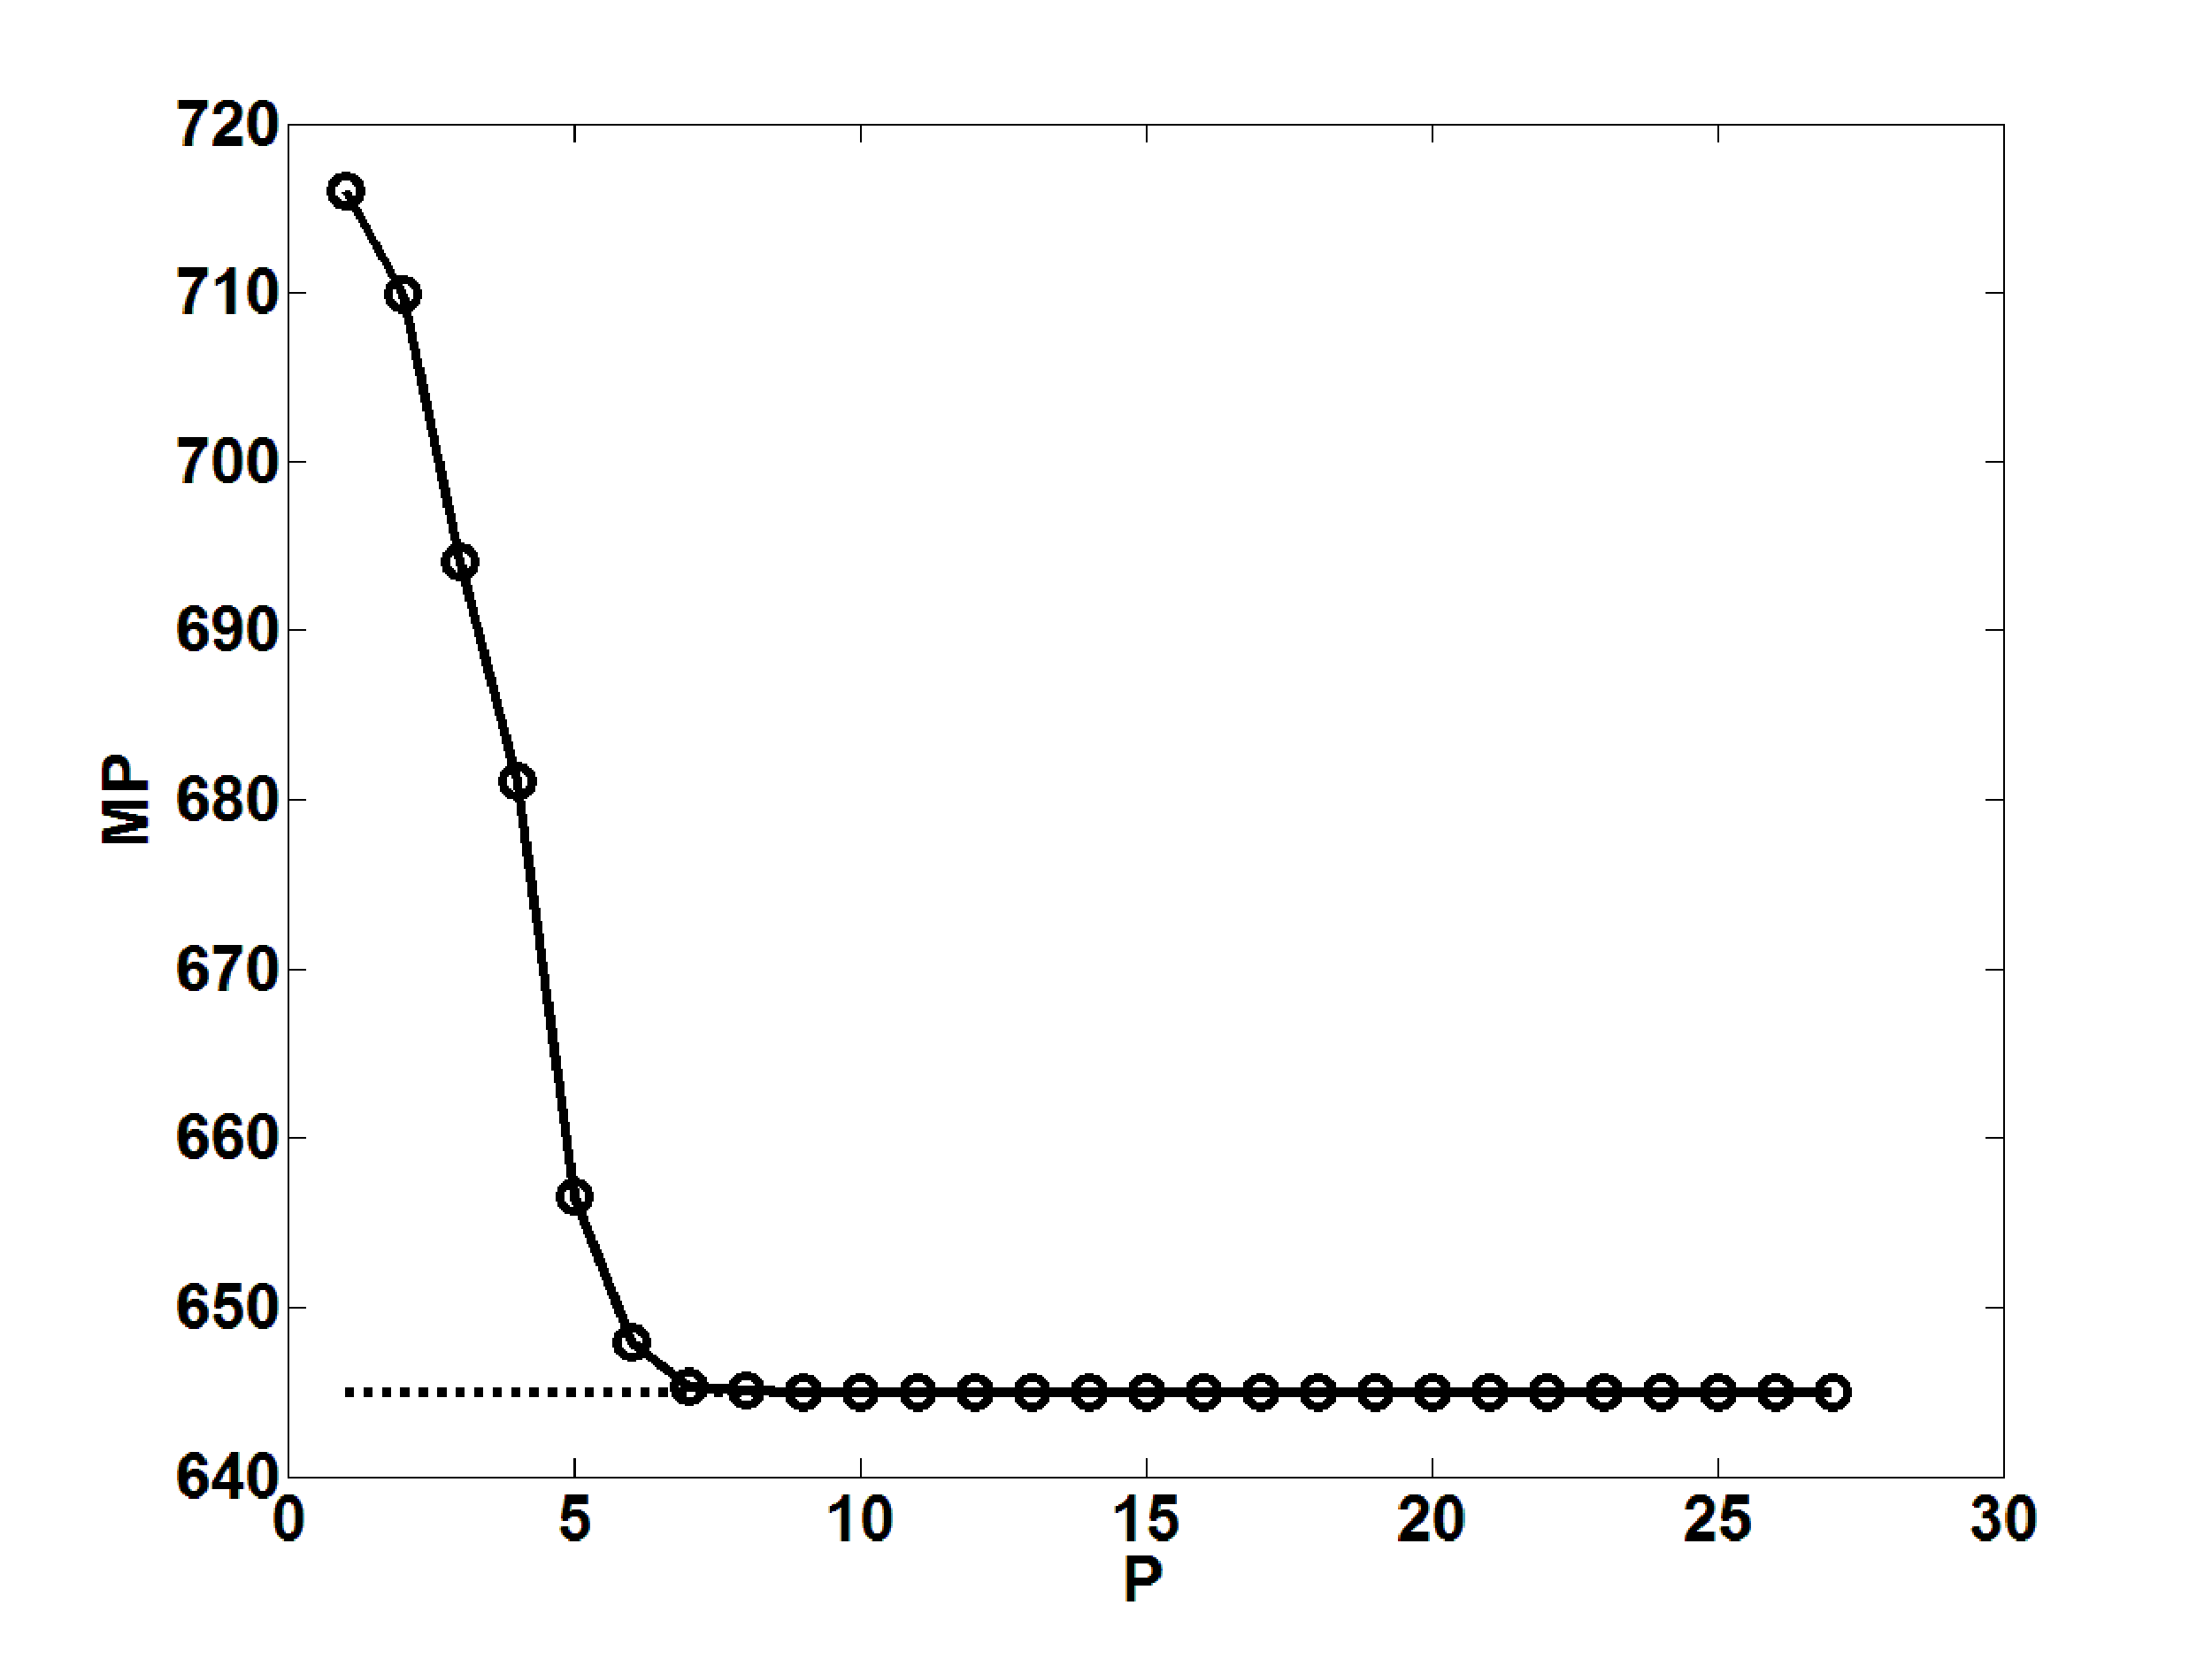
\includegraphics[width=0.3\textwidth]{Miss_logisticoB10}
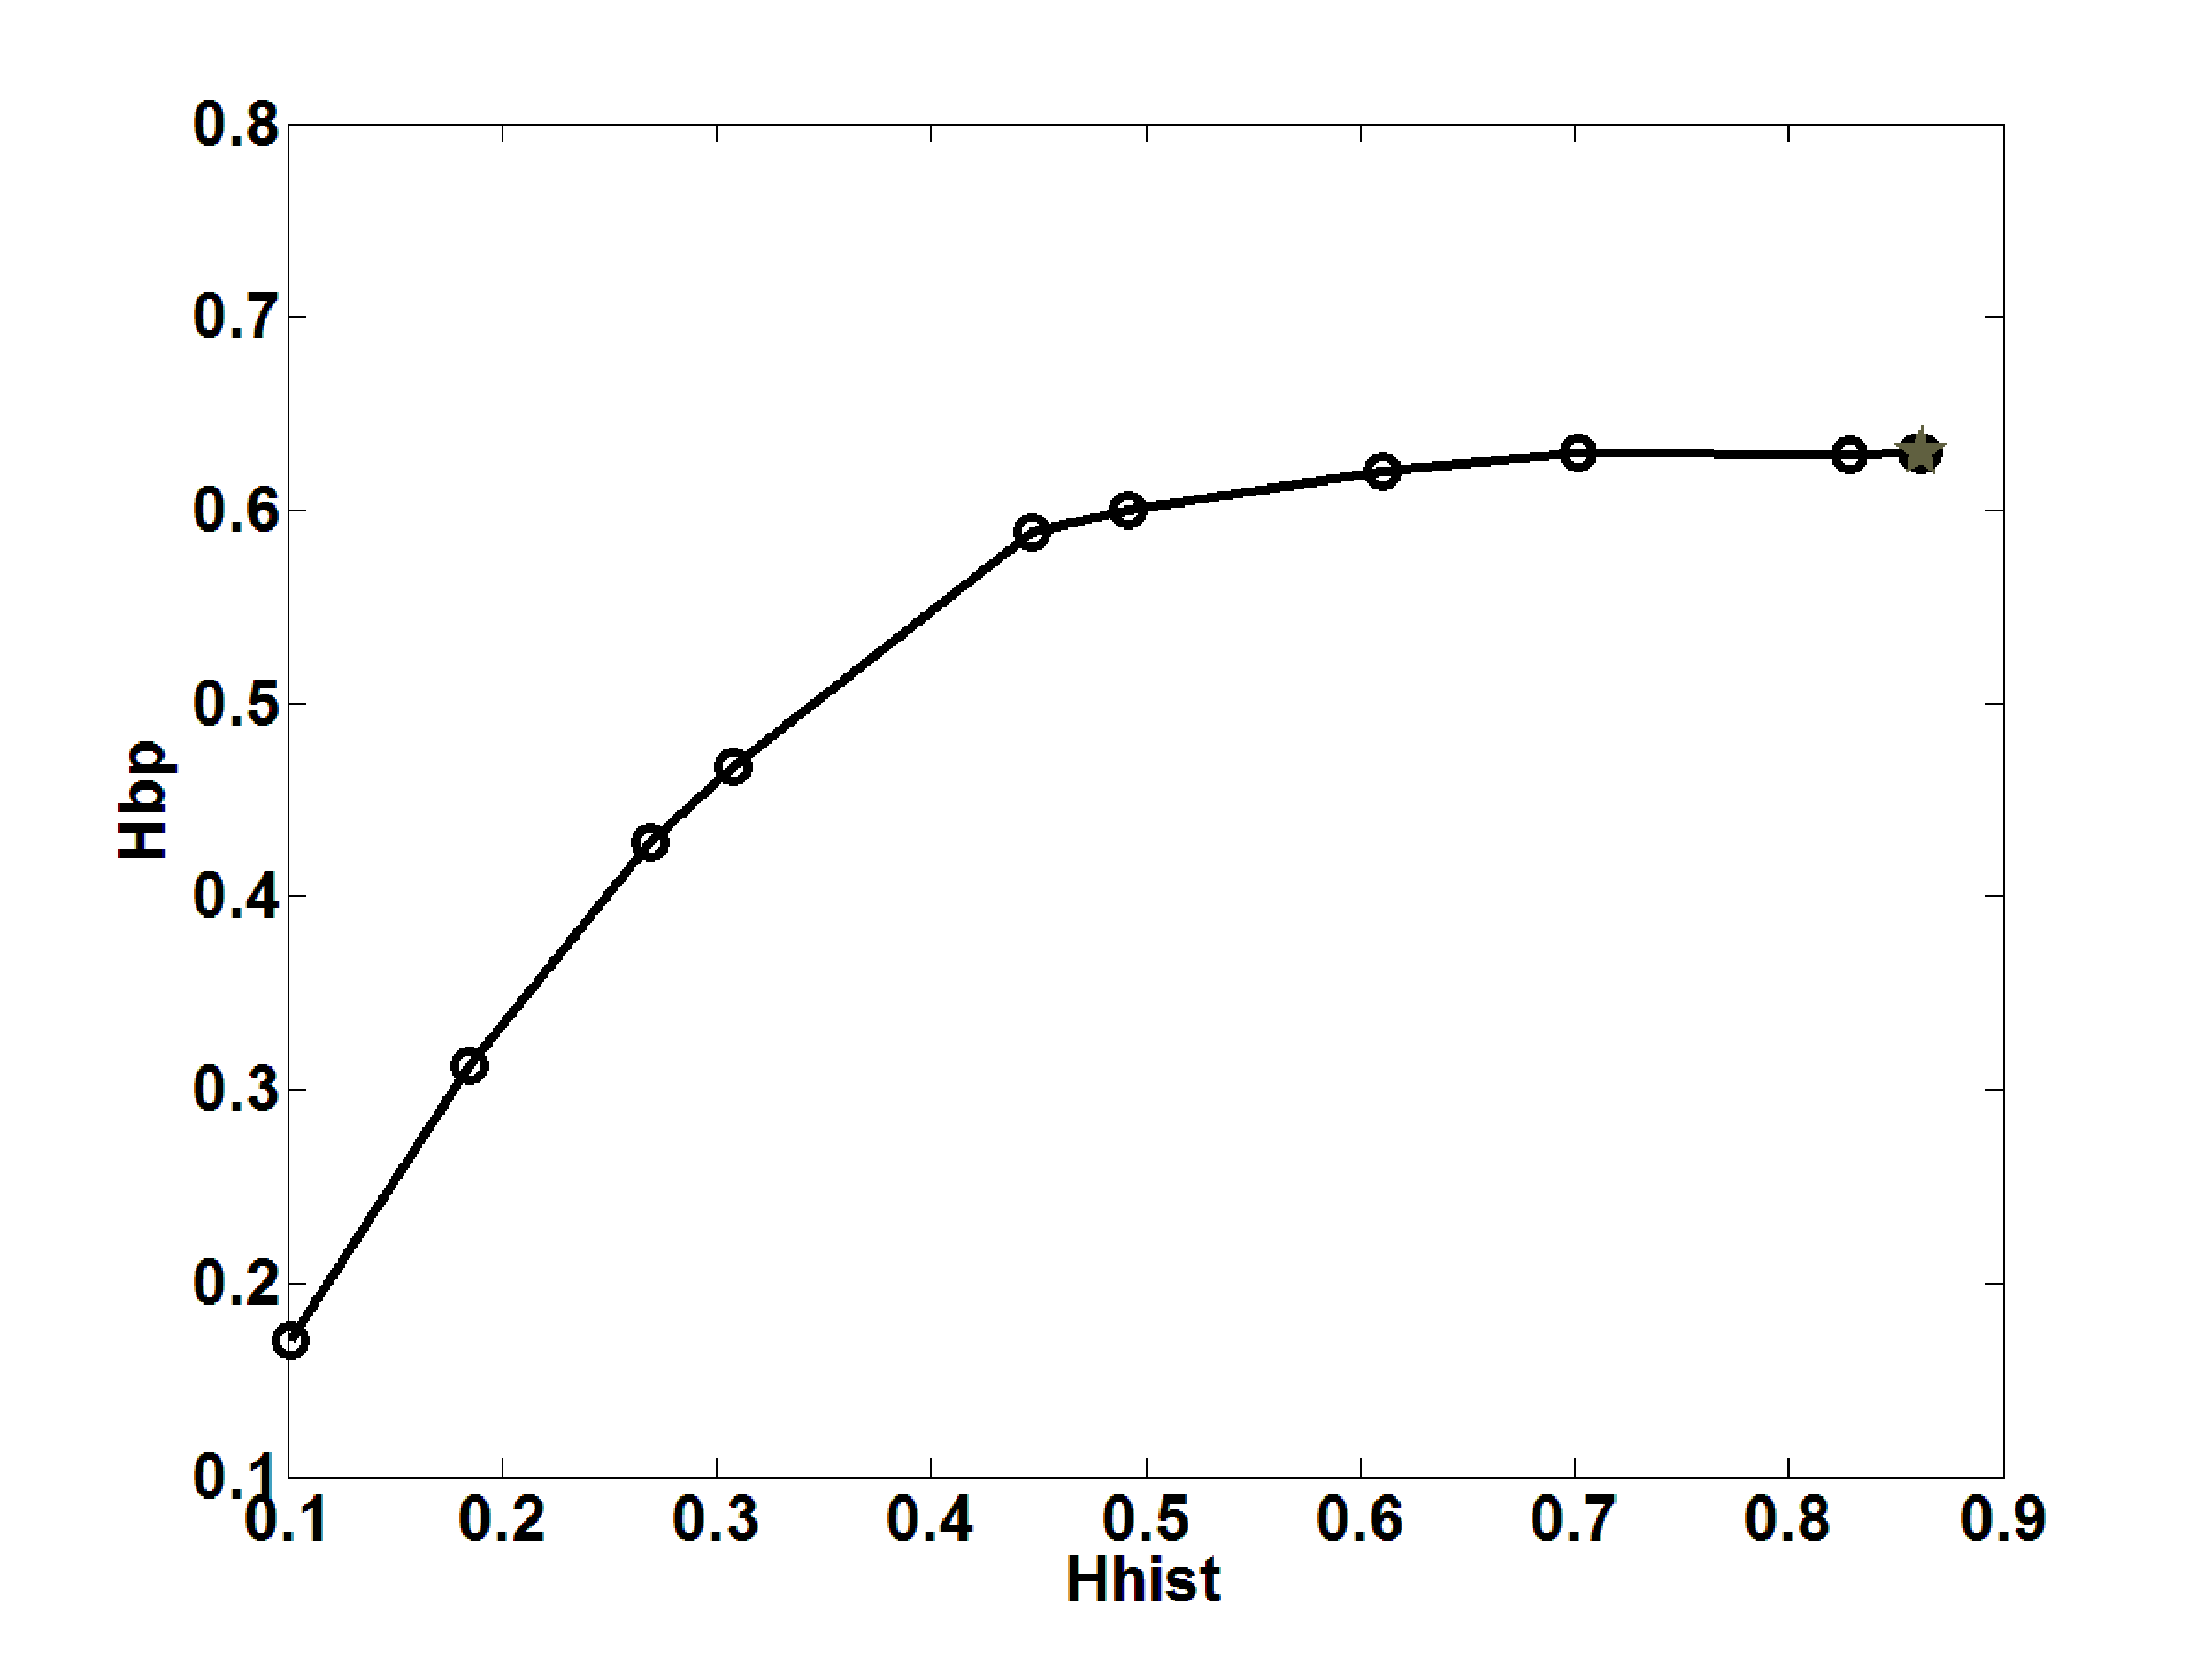
\includegraphics[width=0.3\textwidth]{HhistHbp_logisticoB10}
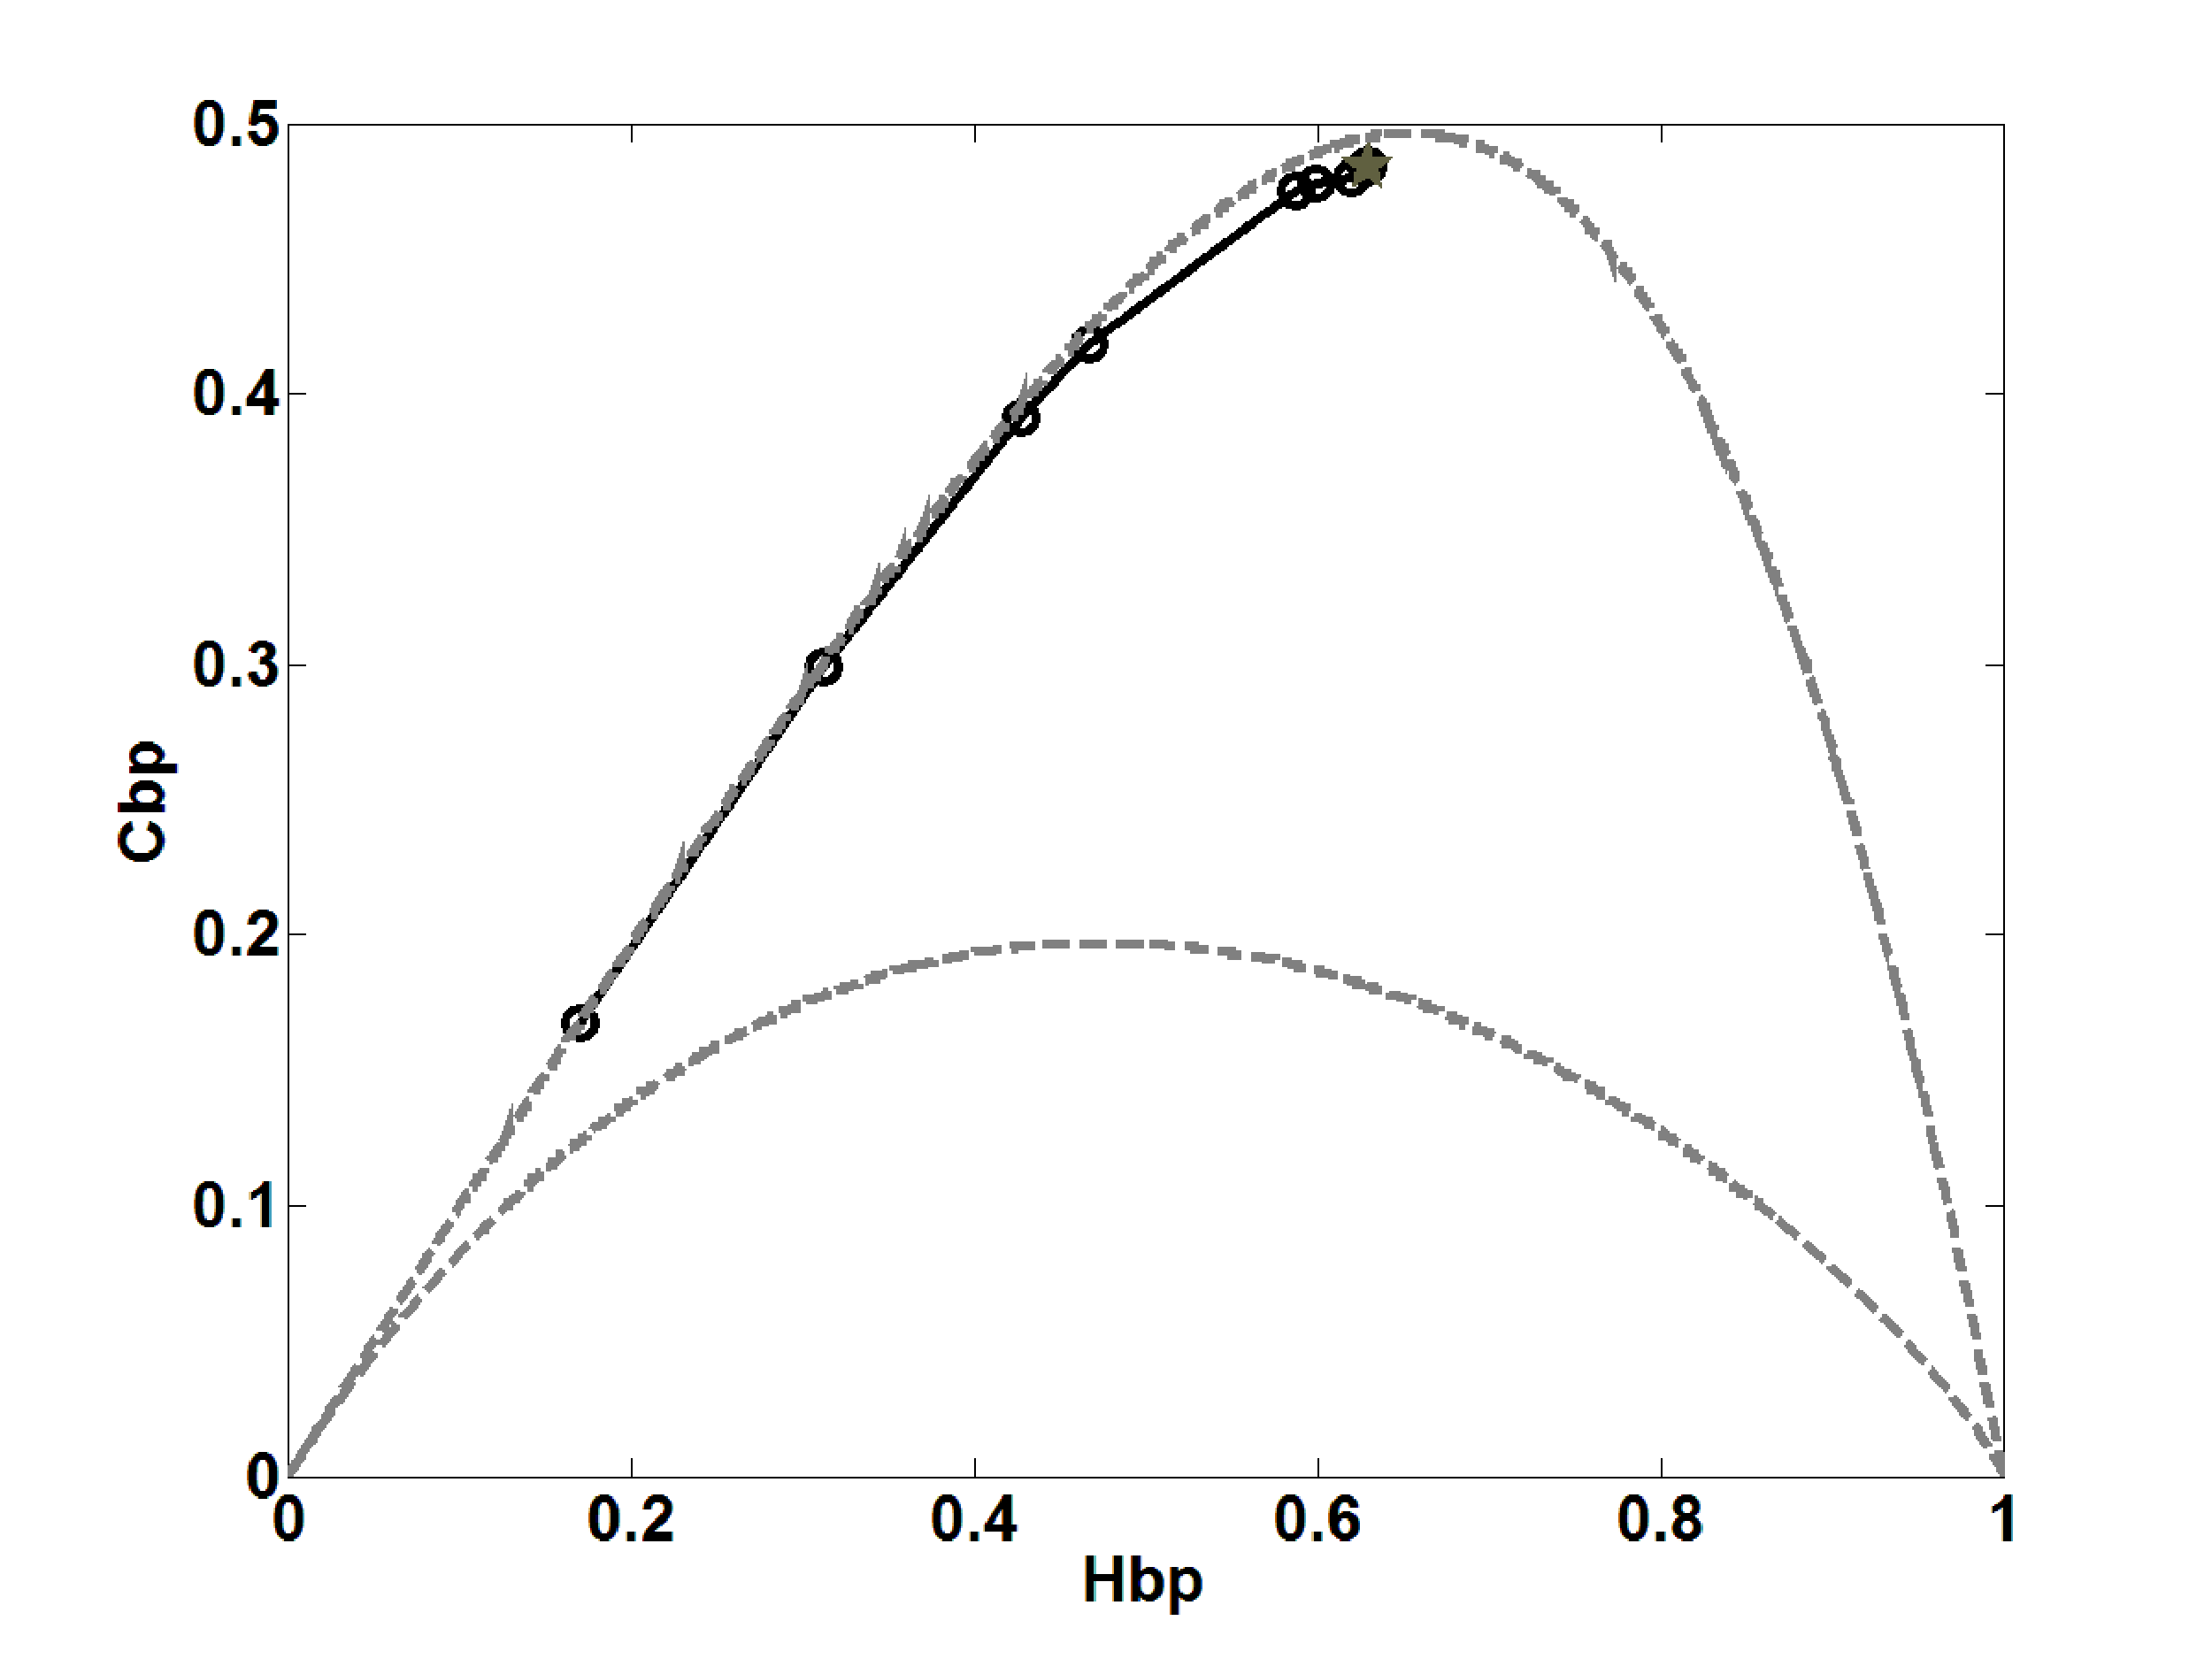
\includegraphics[width=0.3\textwidth]{HbpCbp_logisticoB10}
\caption{Statistical properties of the LOG map using different numerical representations. Figures (a) to(f) correspond to decimal representation: (a) $H_{hist}$ vs $P$ (b) $H_{BP}$ vs $P$ (c) $C_{BP}$ vs $P$ (d) Number of missing ordering patterns $MP$ vs $P$. In Figures (a) to (d) dashed line correspond to floating point numbers. (d) representation in the $H_{hist},H_{BP}$ plane in the the decimal numerical system.  The star represents the state for floating points numbers. (e) representation in the $H_{hist},H_{BP}$ plane. The star represents the state for floating point numbers; (f) representation in the $H_{BP},C_{BP}$ plane.  The star represents the state for floating points numbers. (f) representation in the $H_{BP},C_{BP}$ plane for binary numerical system.  The star represents the state for floating points numbers. } \label{fig:LOGdecimal}
\end{figure}
%%%%%%%%%%%%%%%%%%%%%%%%%%
%%%%%%%%%%%%%%%%%%%%%%%%%%% Fig.4
\begin{figure}
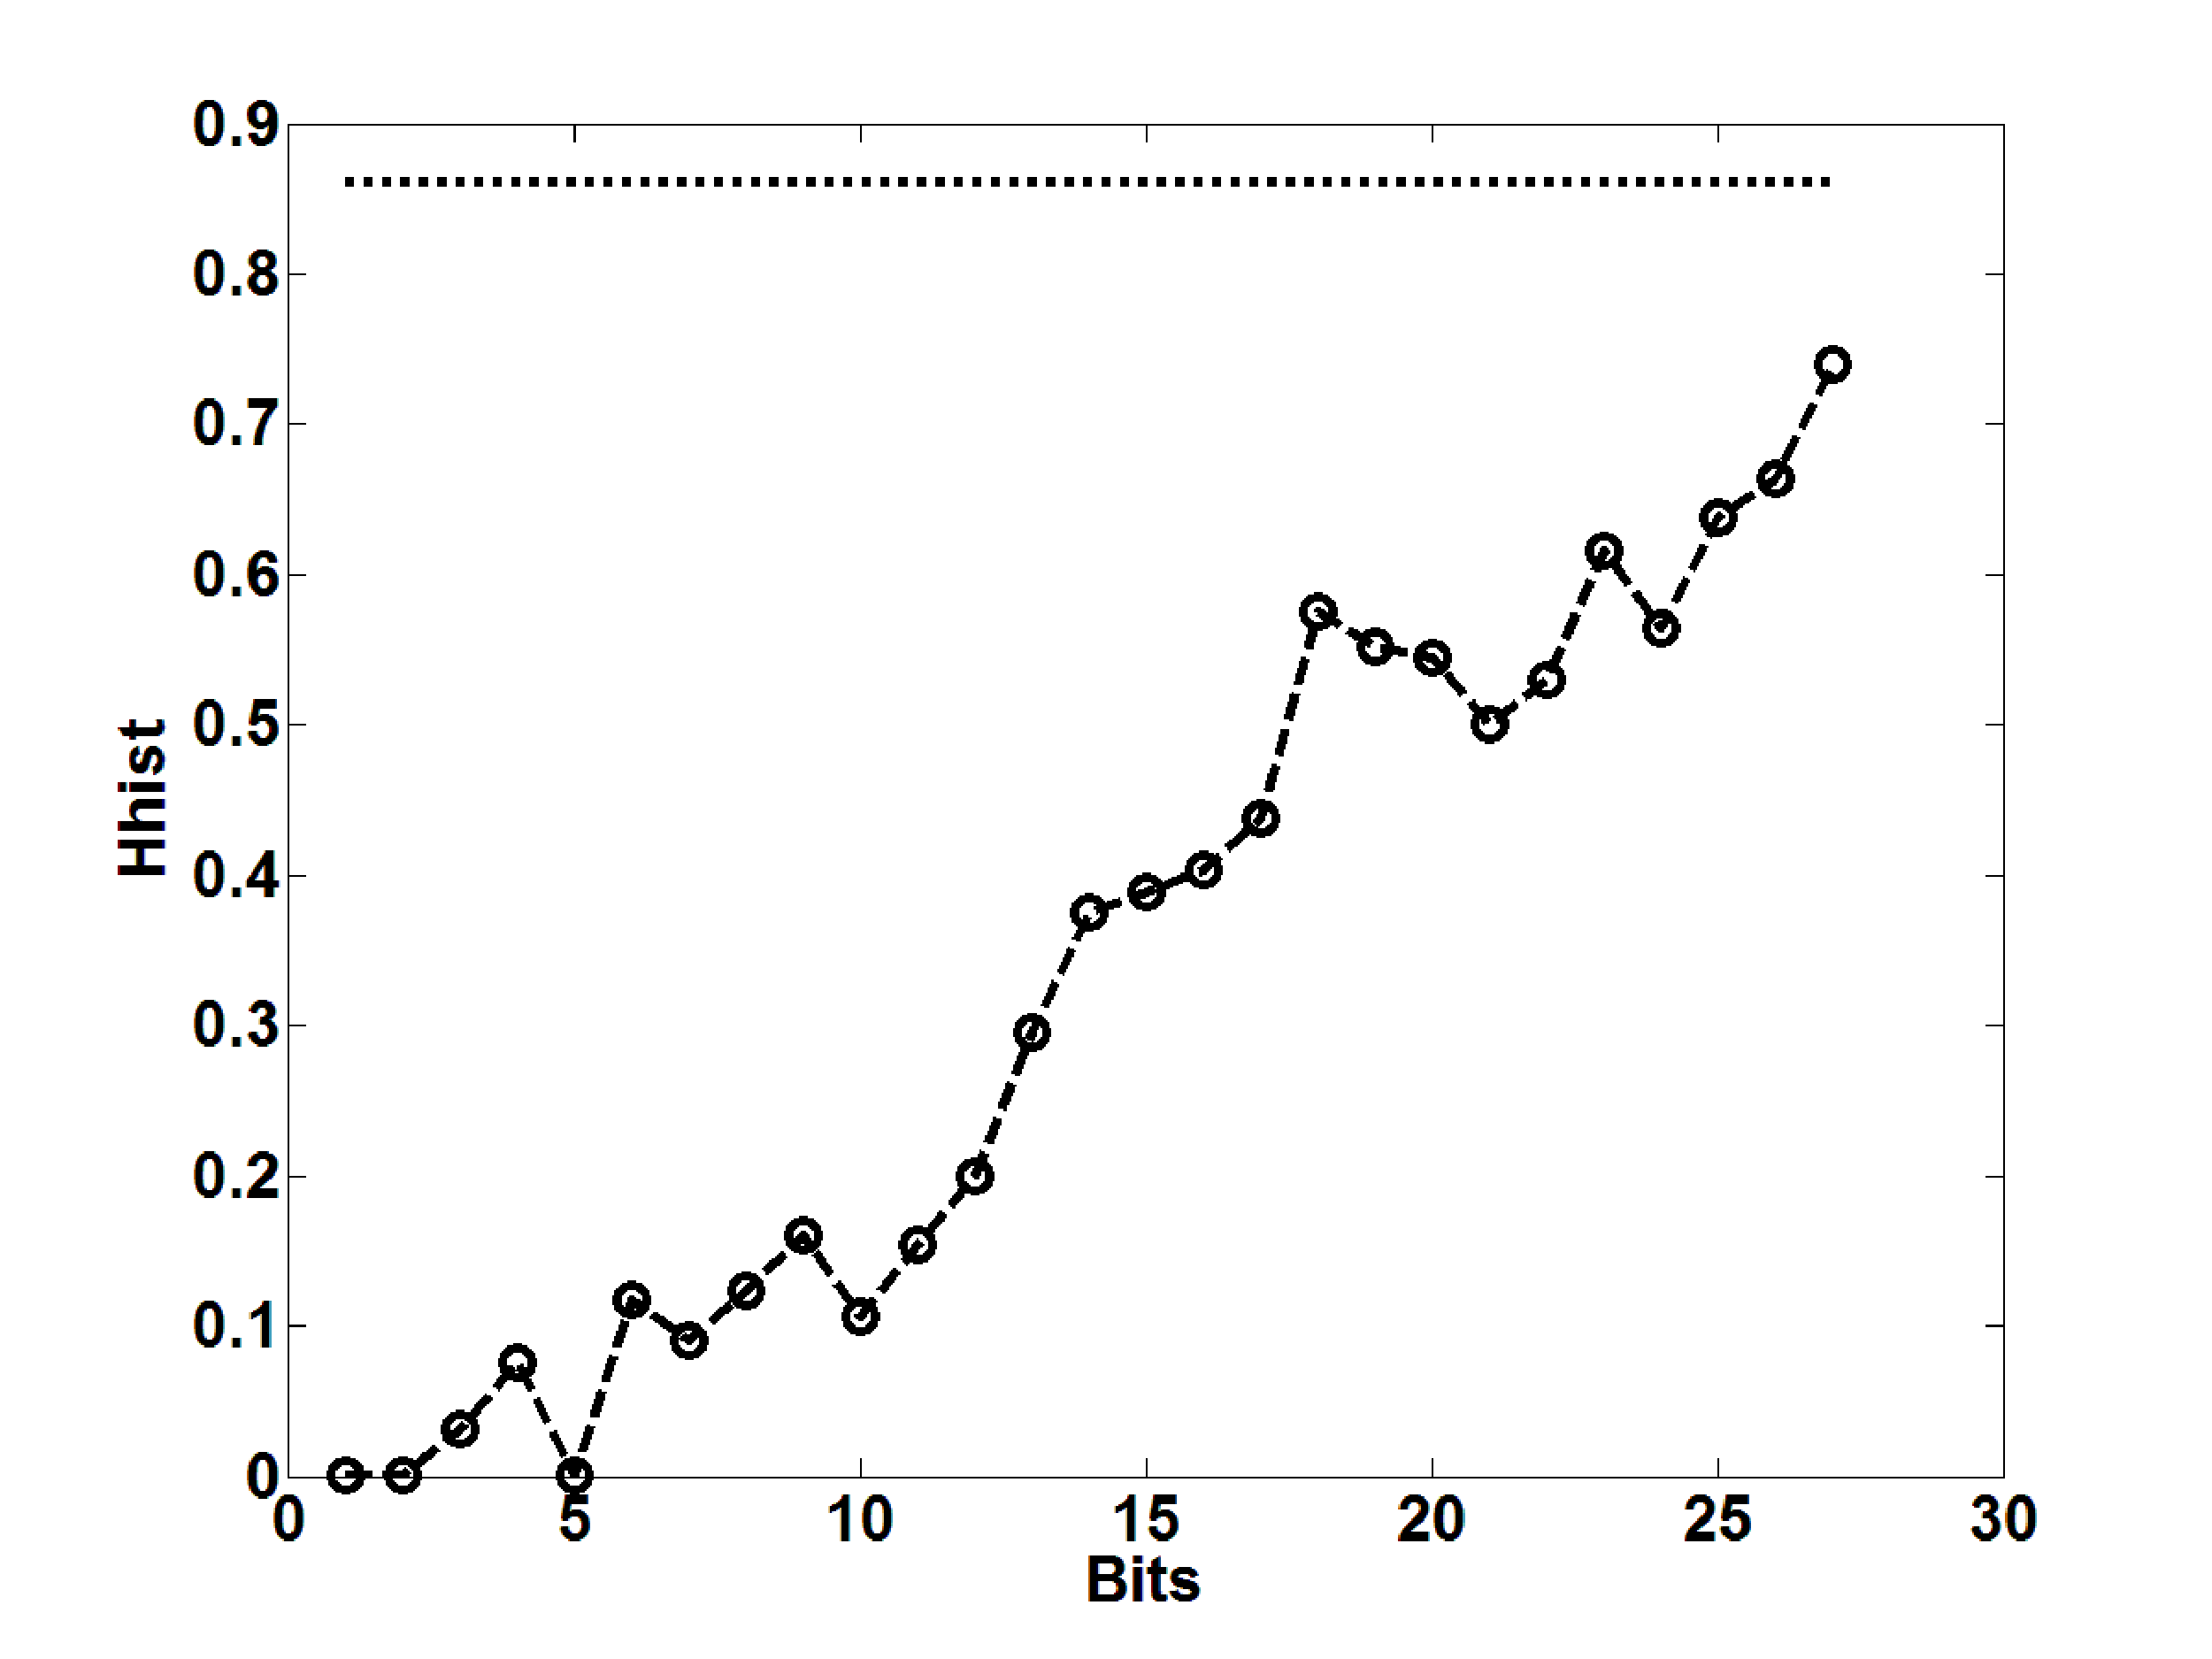
\includegraphics[width=0.3\textwidth]{Hhist_logisticoB2}
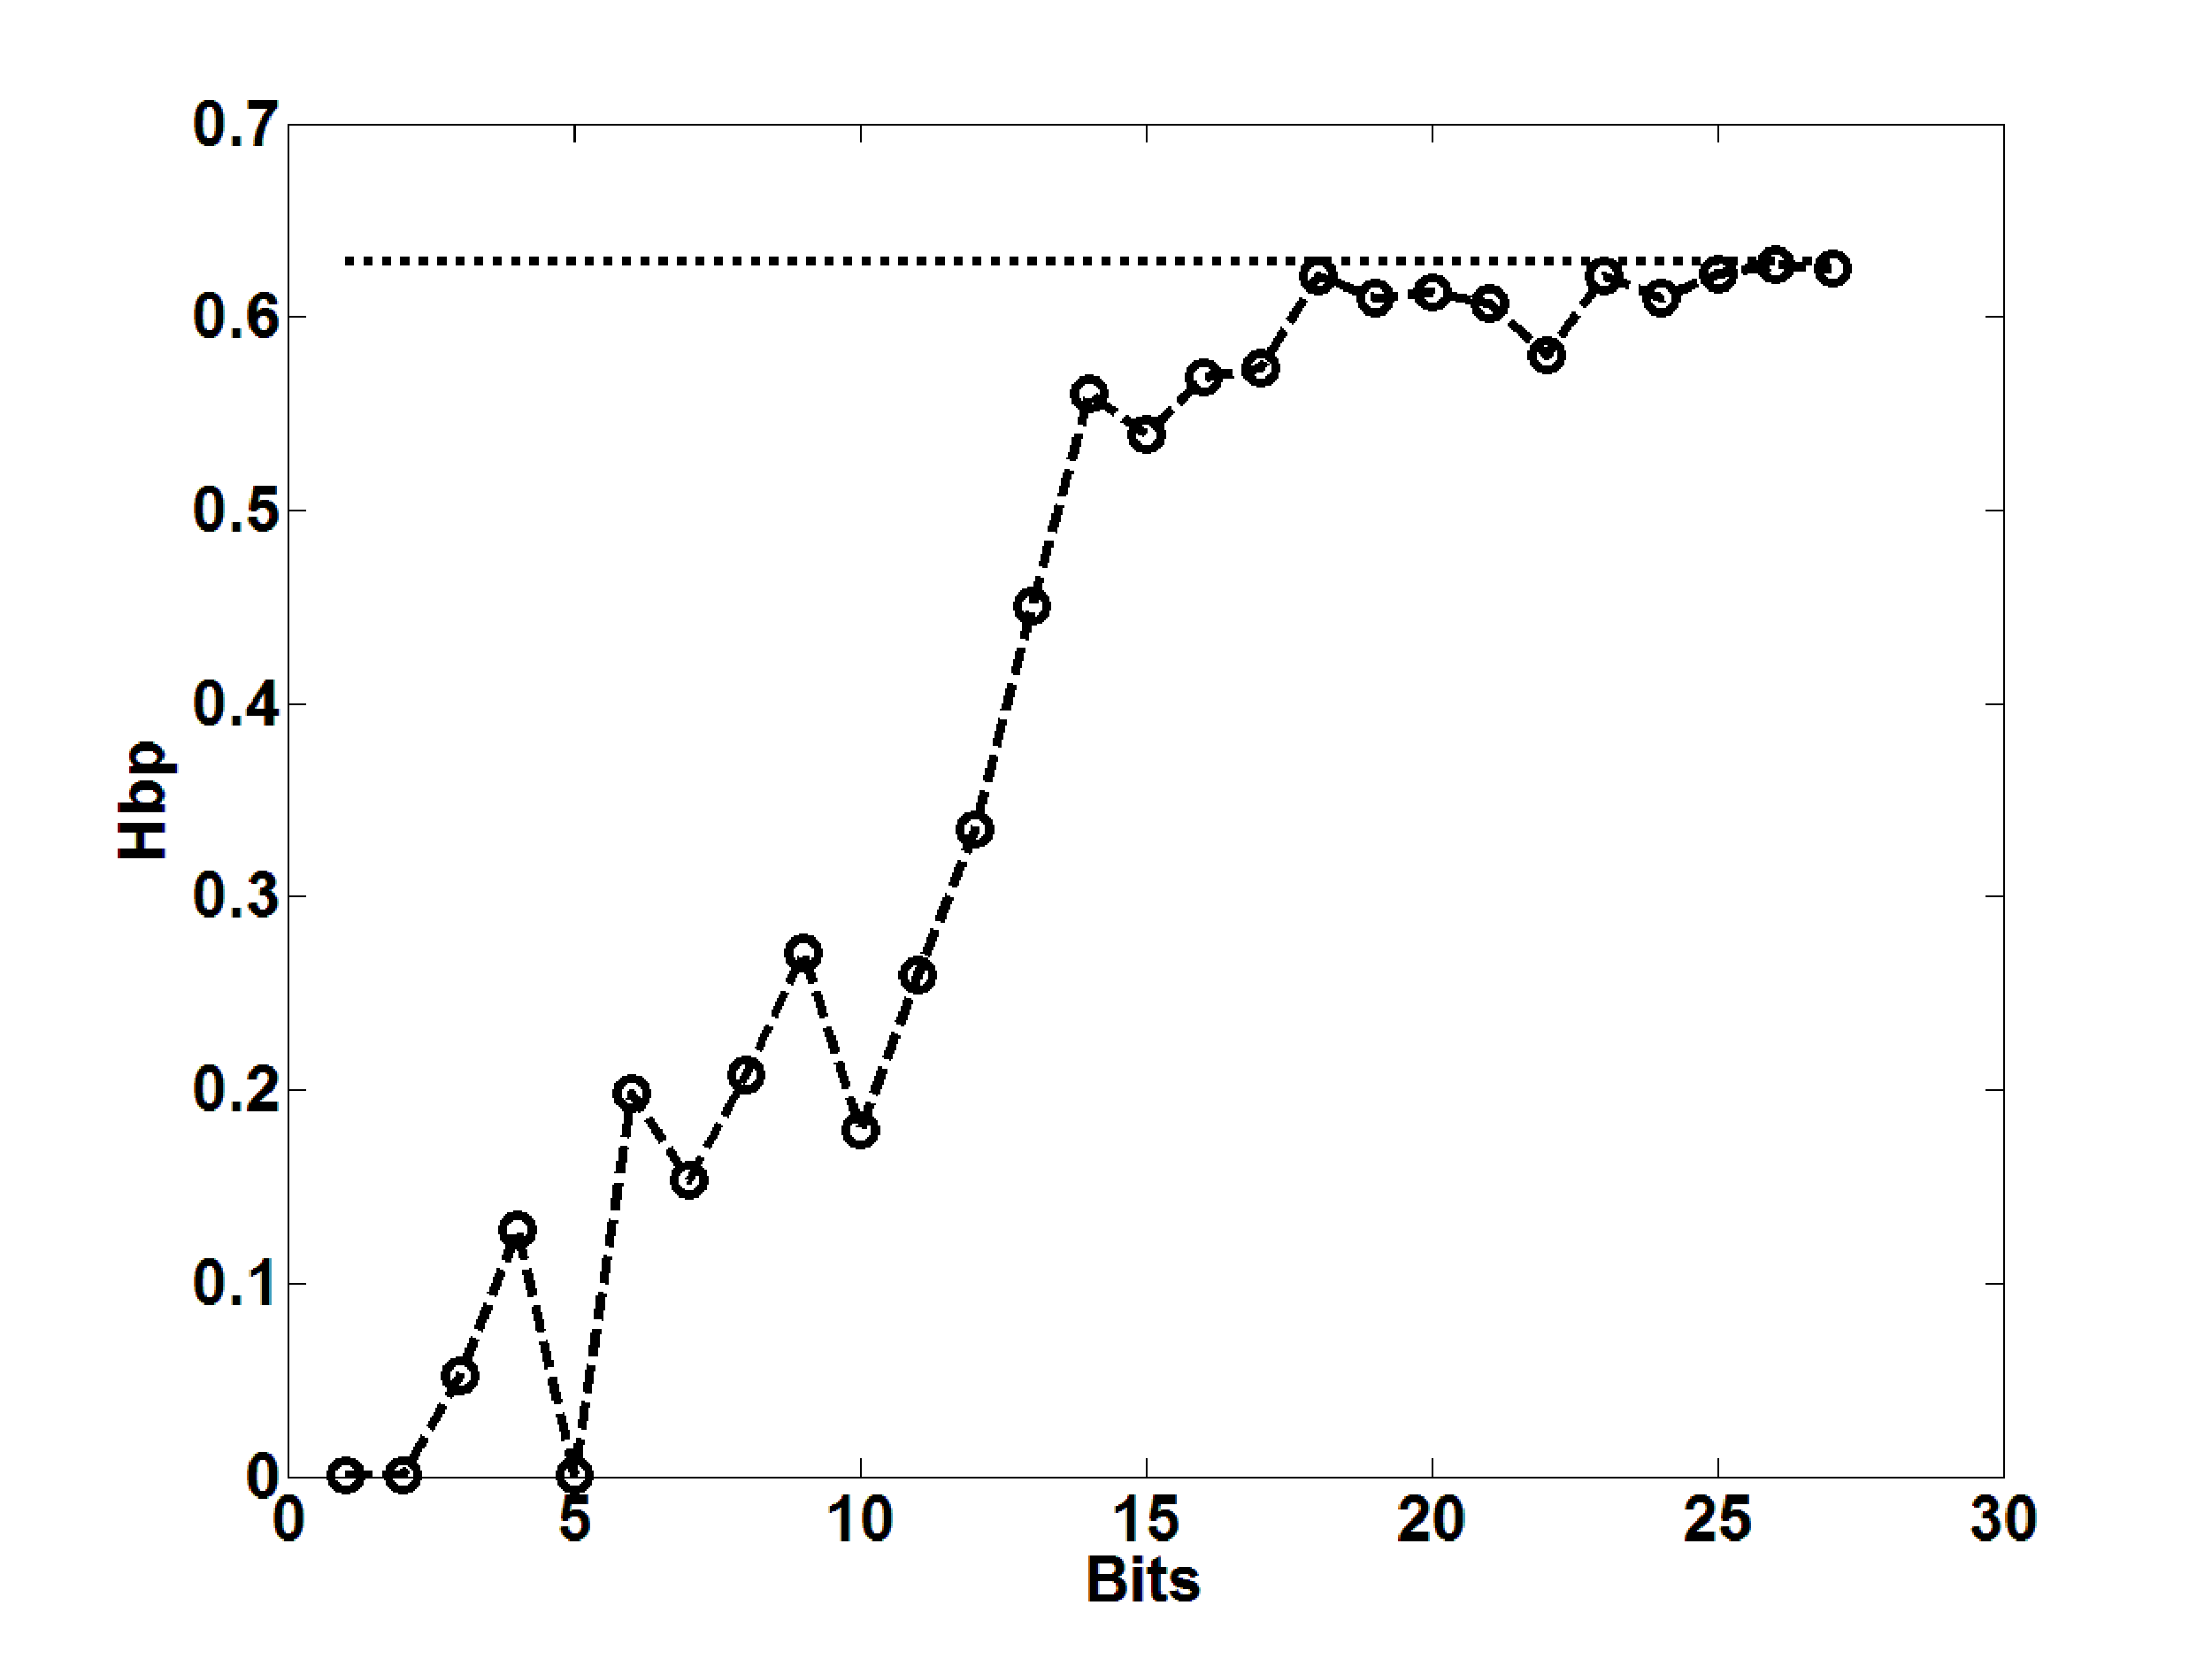
\includegraphics[width=0.3\textwidth]{Hbp_logisticoB2}
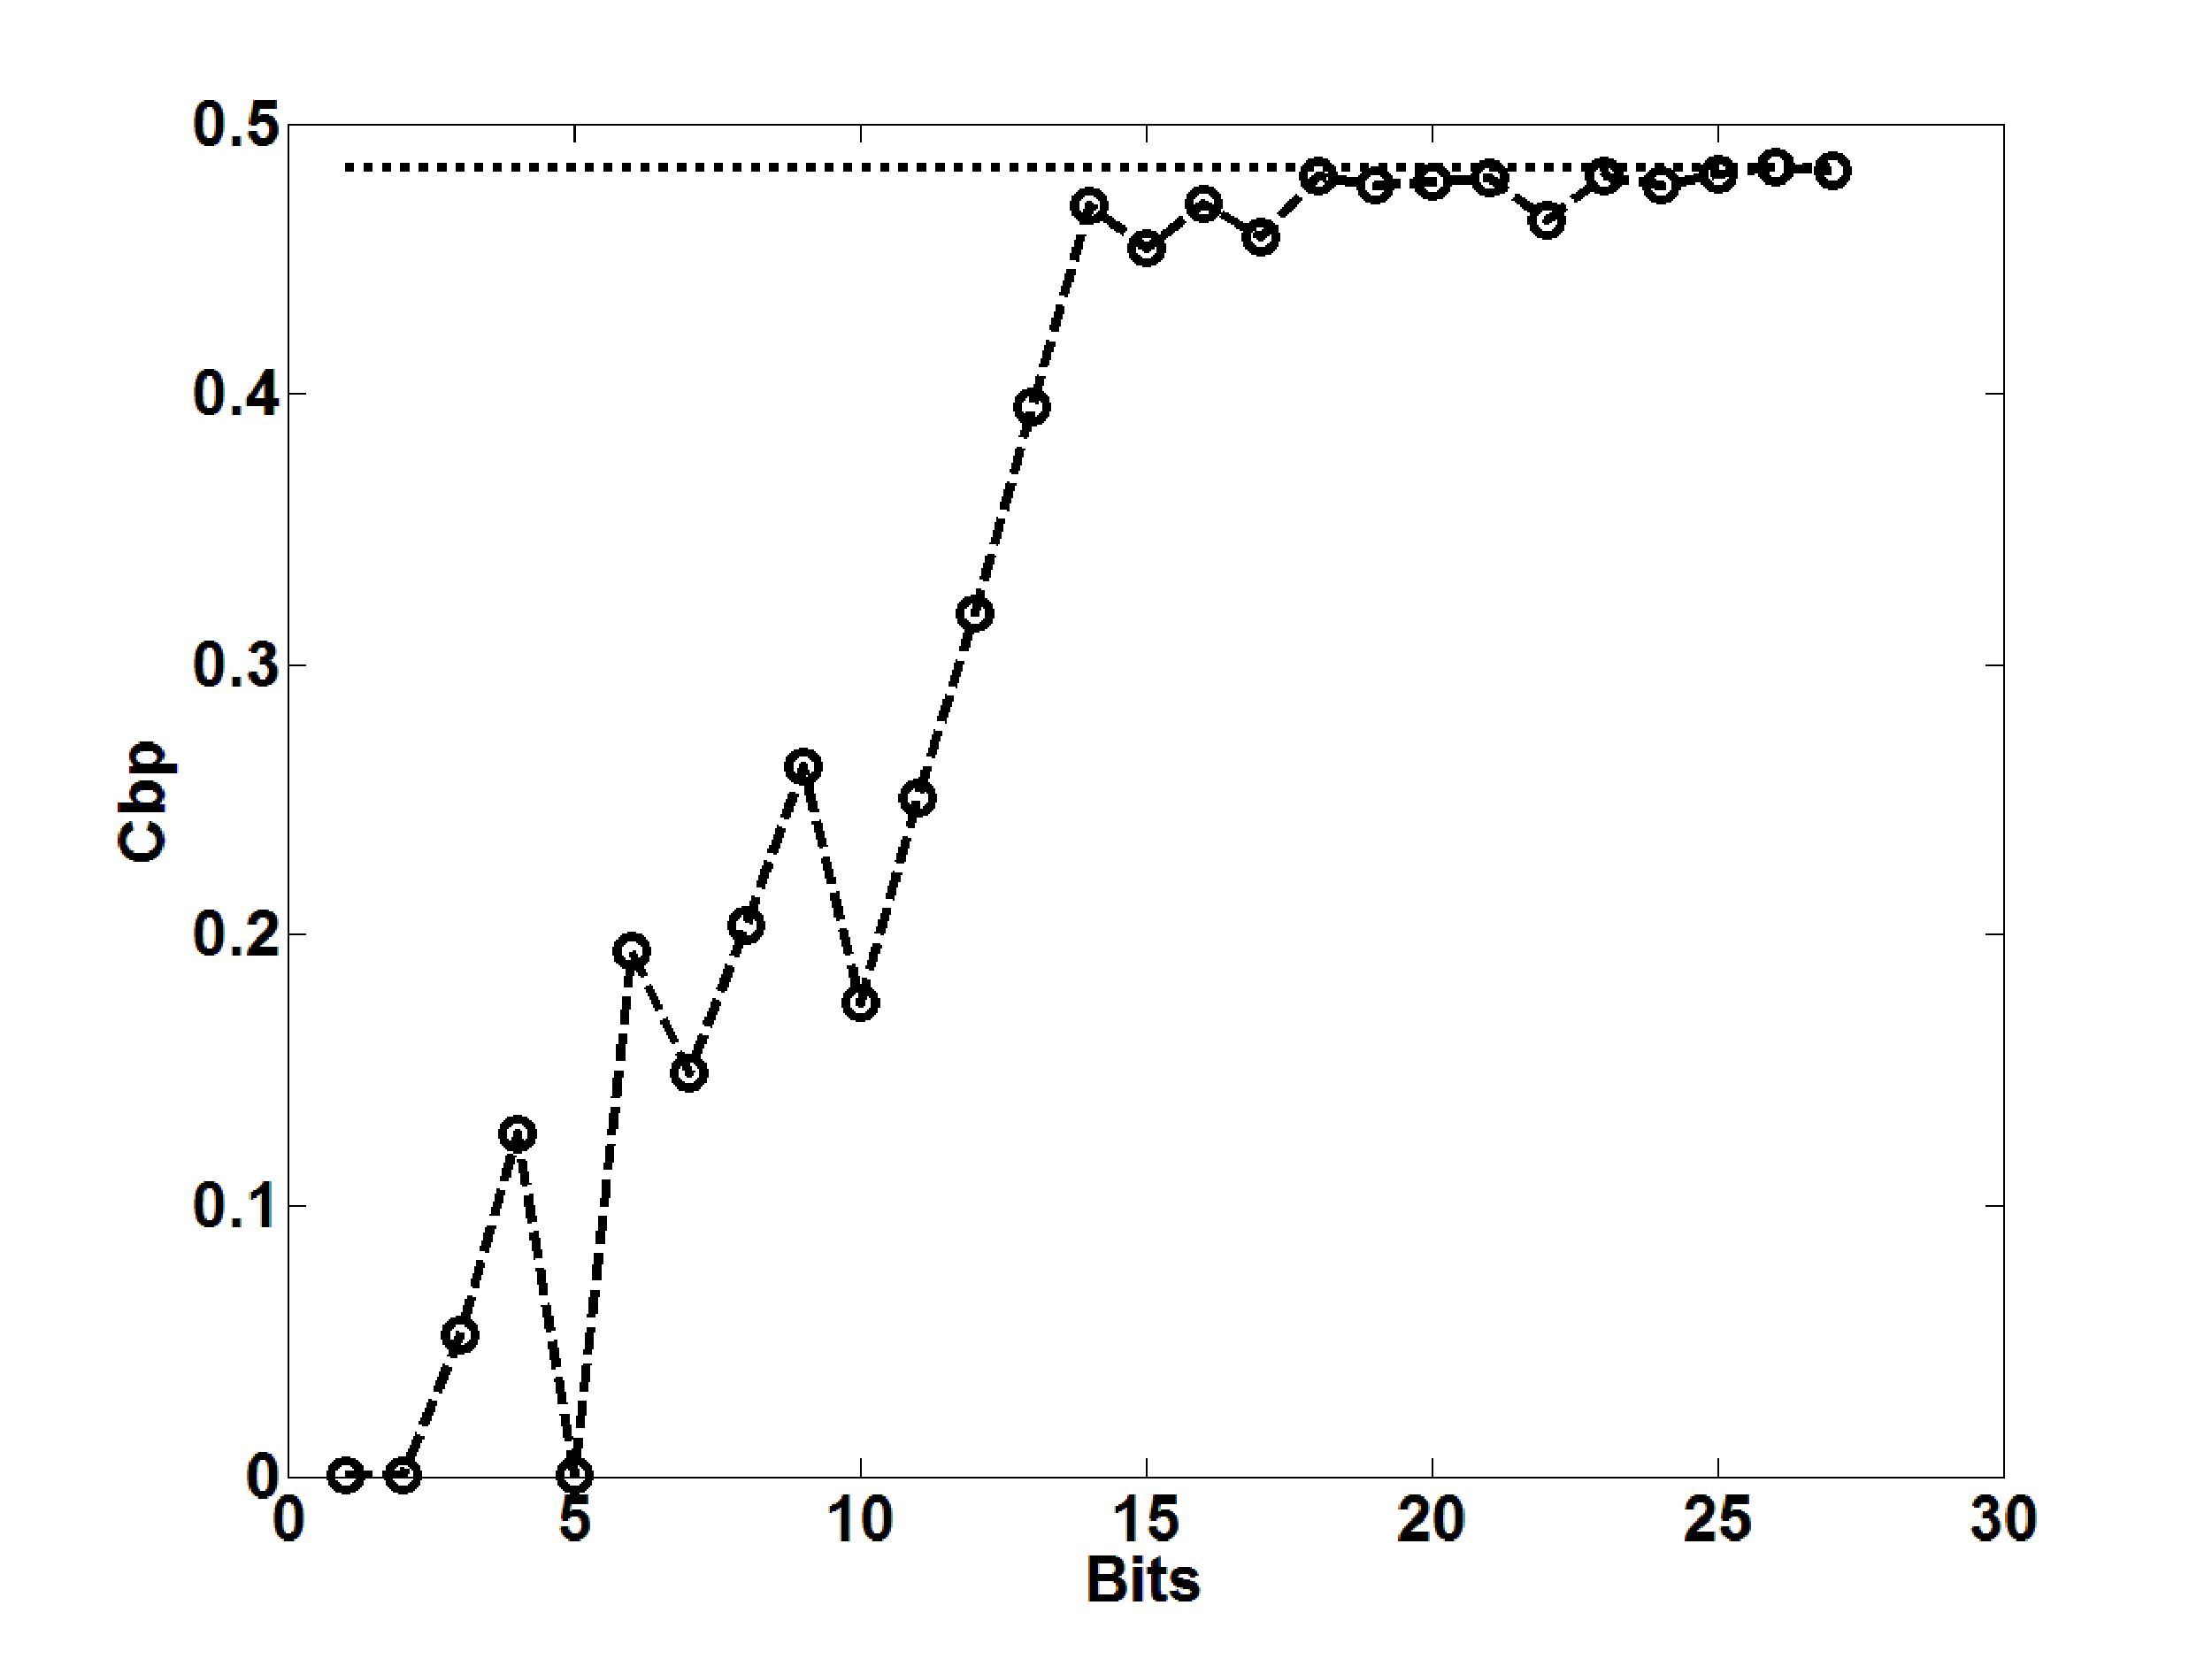
\includegraphics[width=0.3\textwidth]{Cbp_logisticoB2}
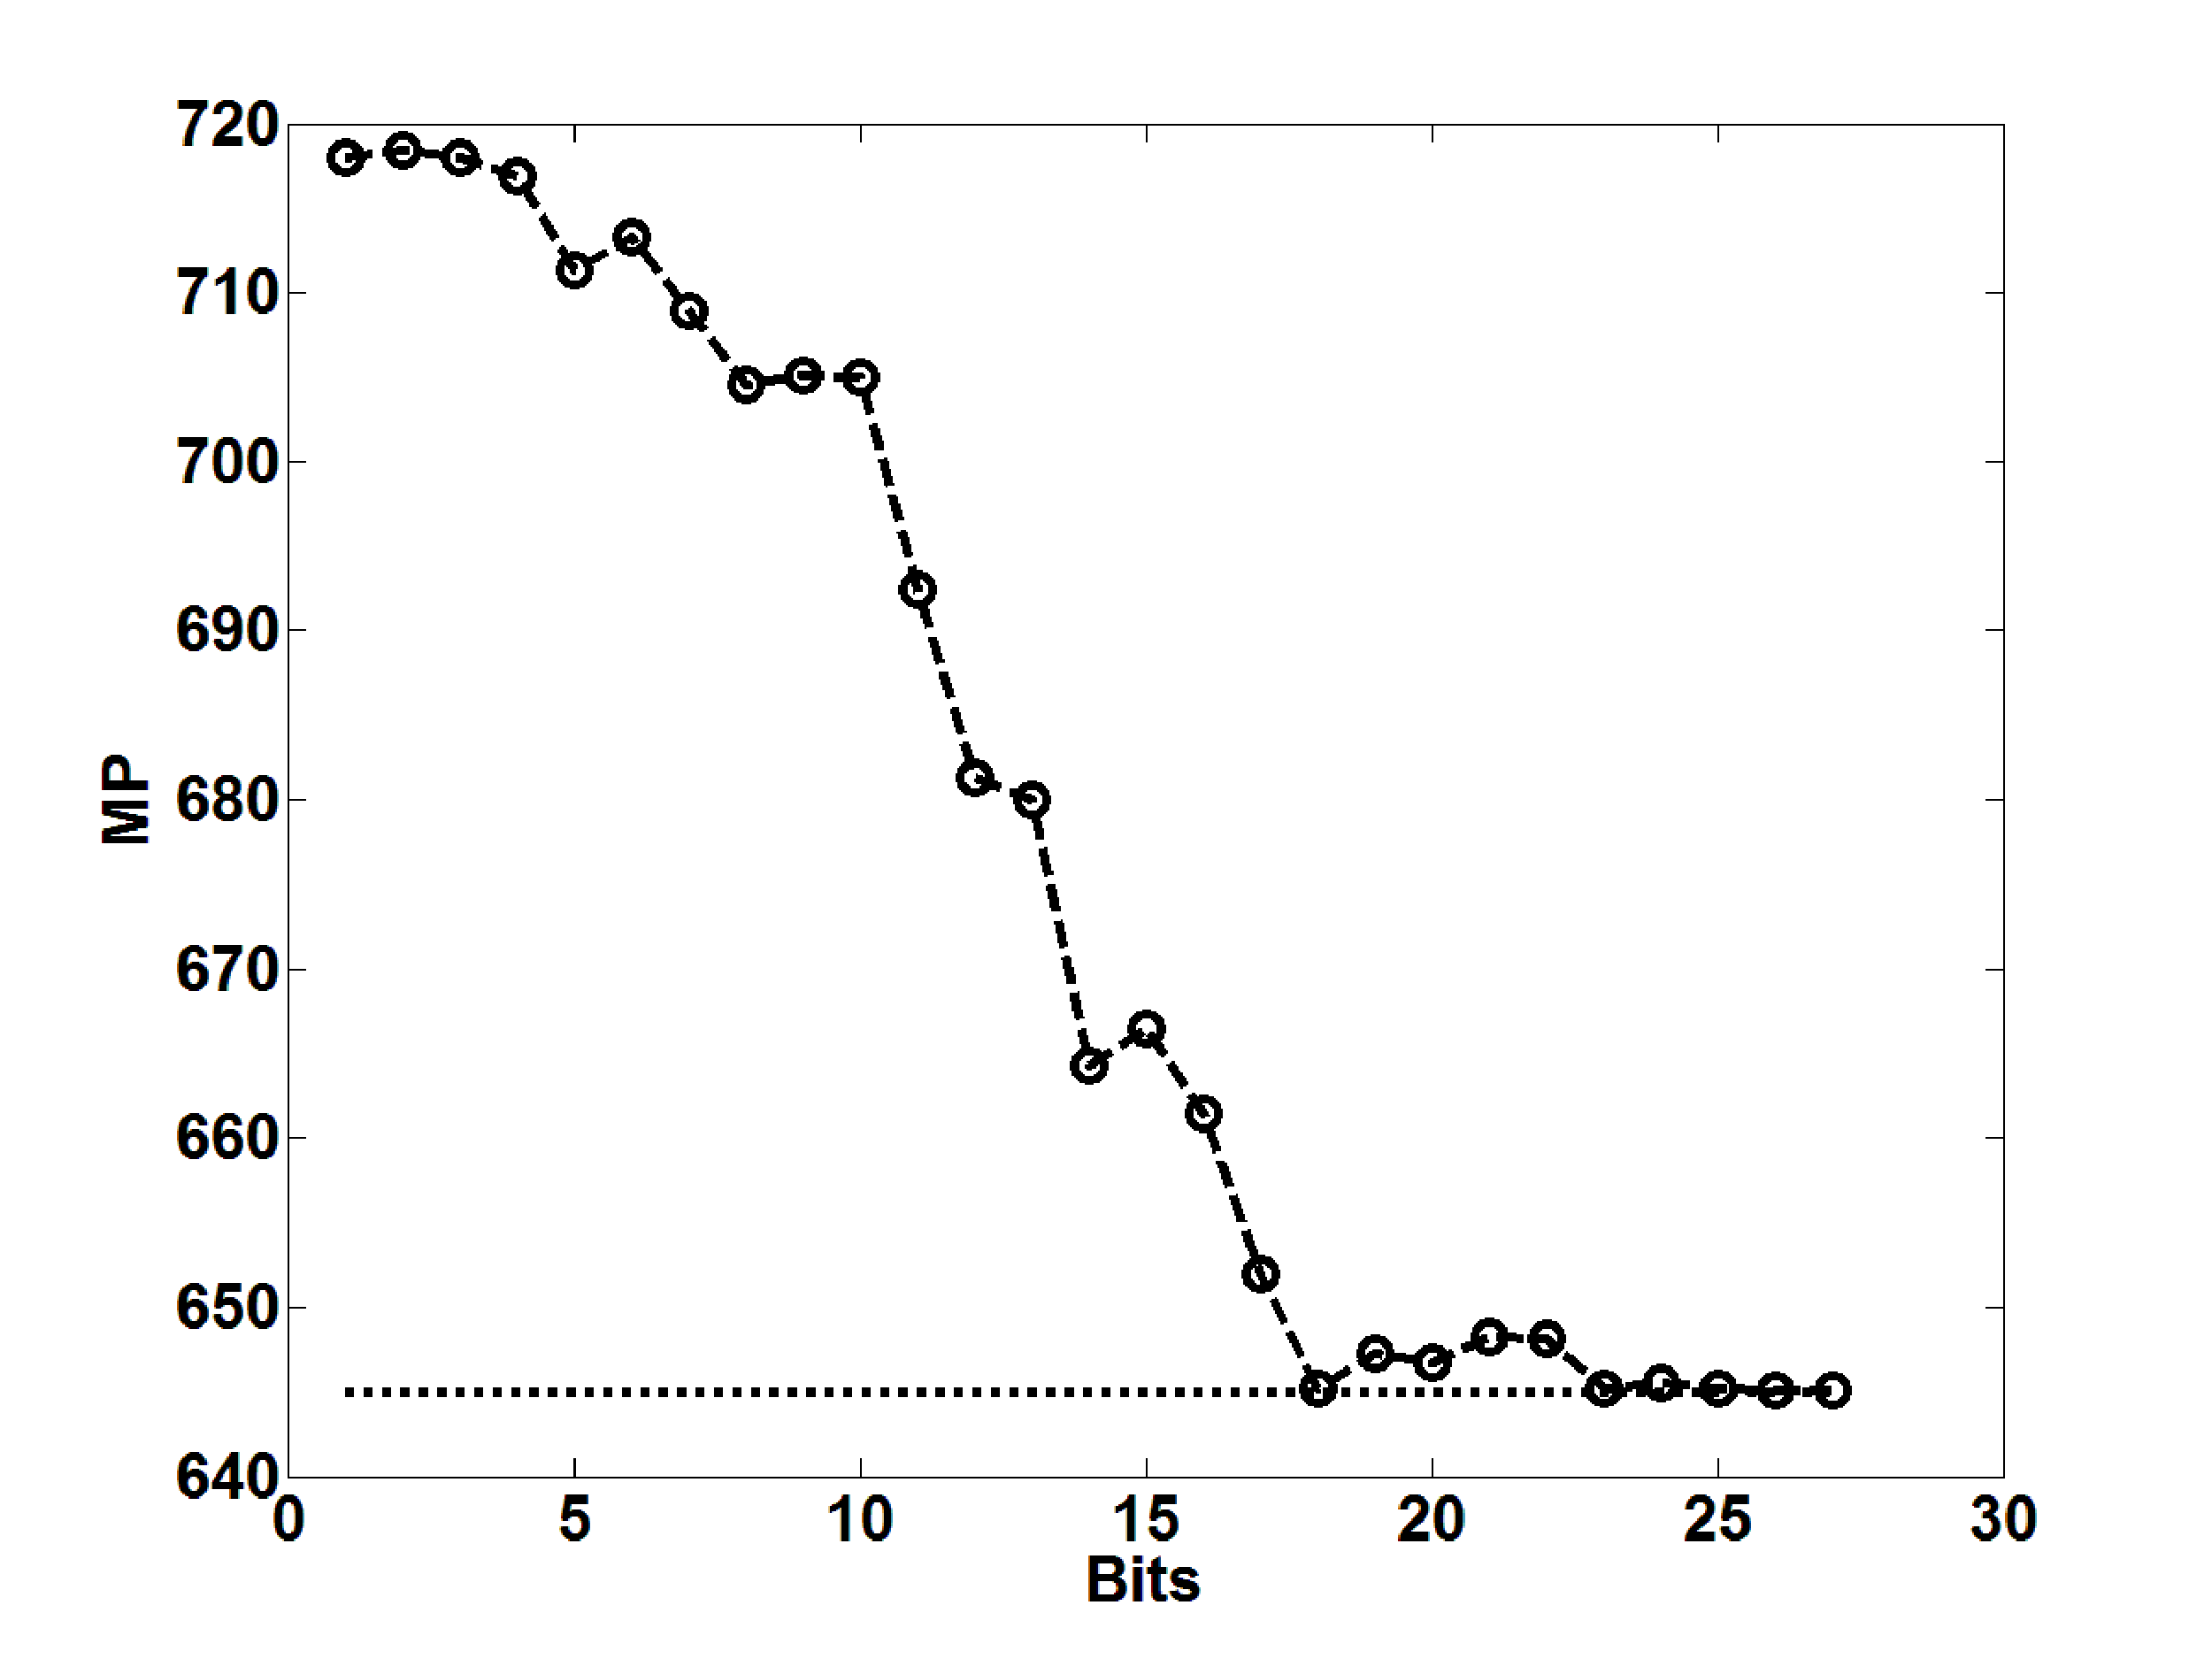
\includegraphics[width=0.3\textwidth]{Miss_logisticoB2}
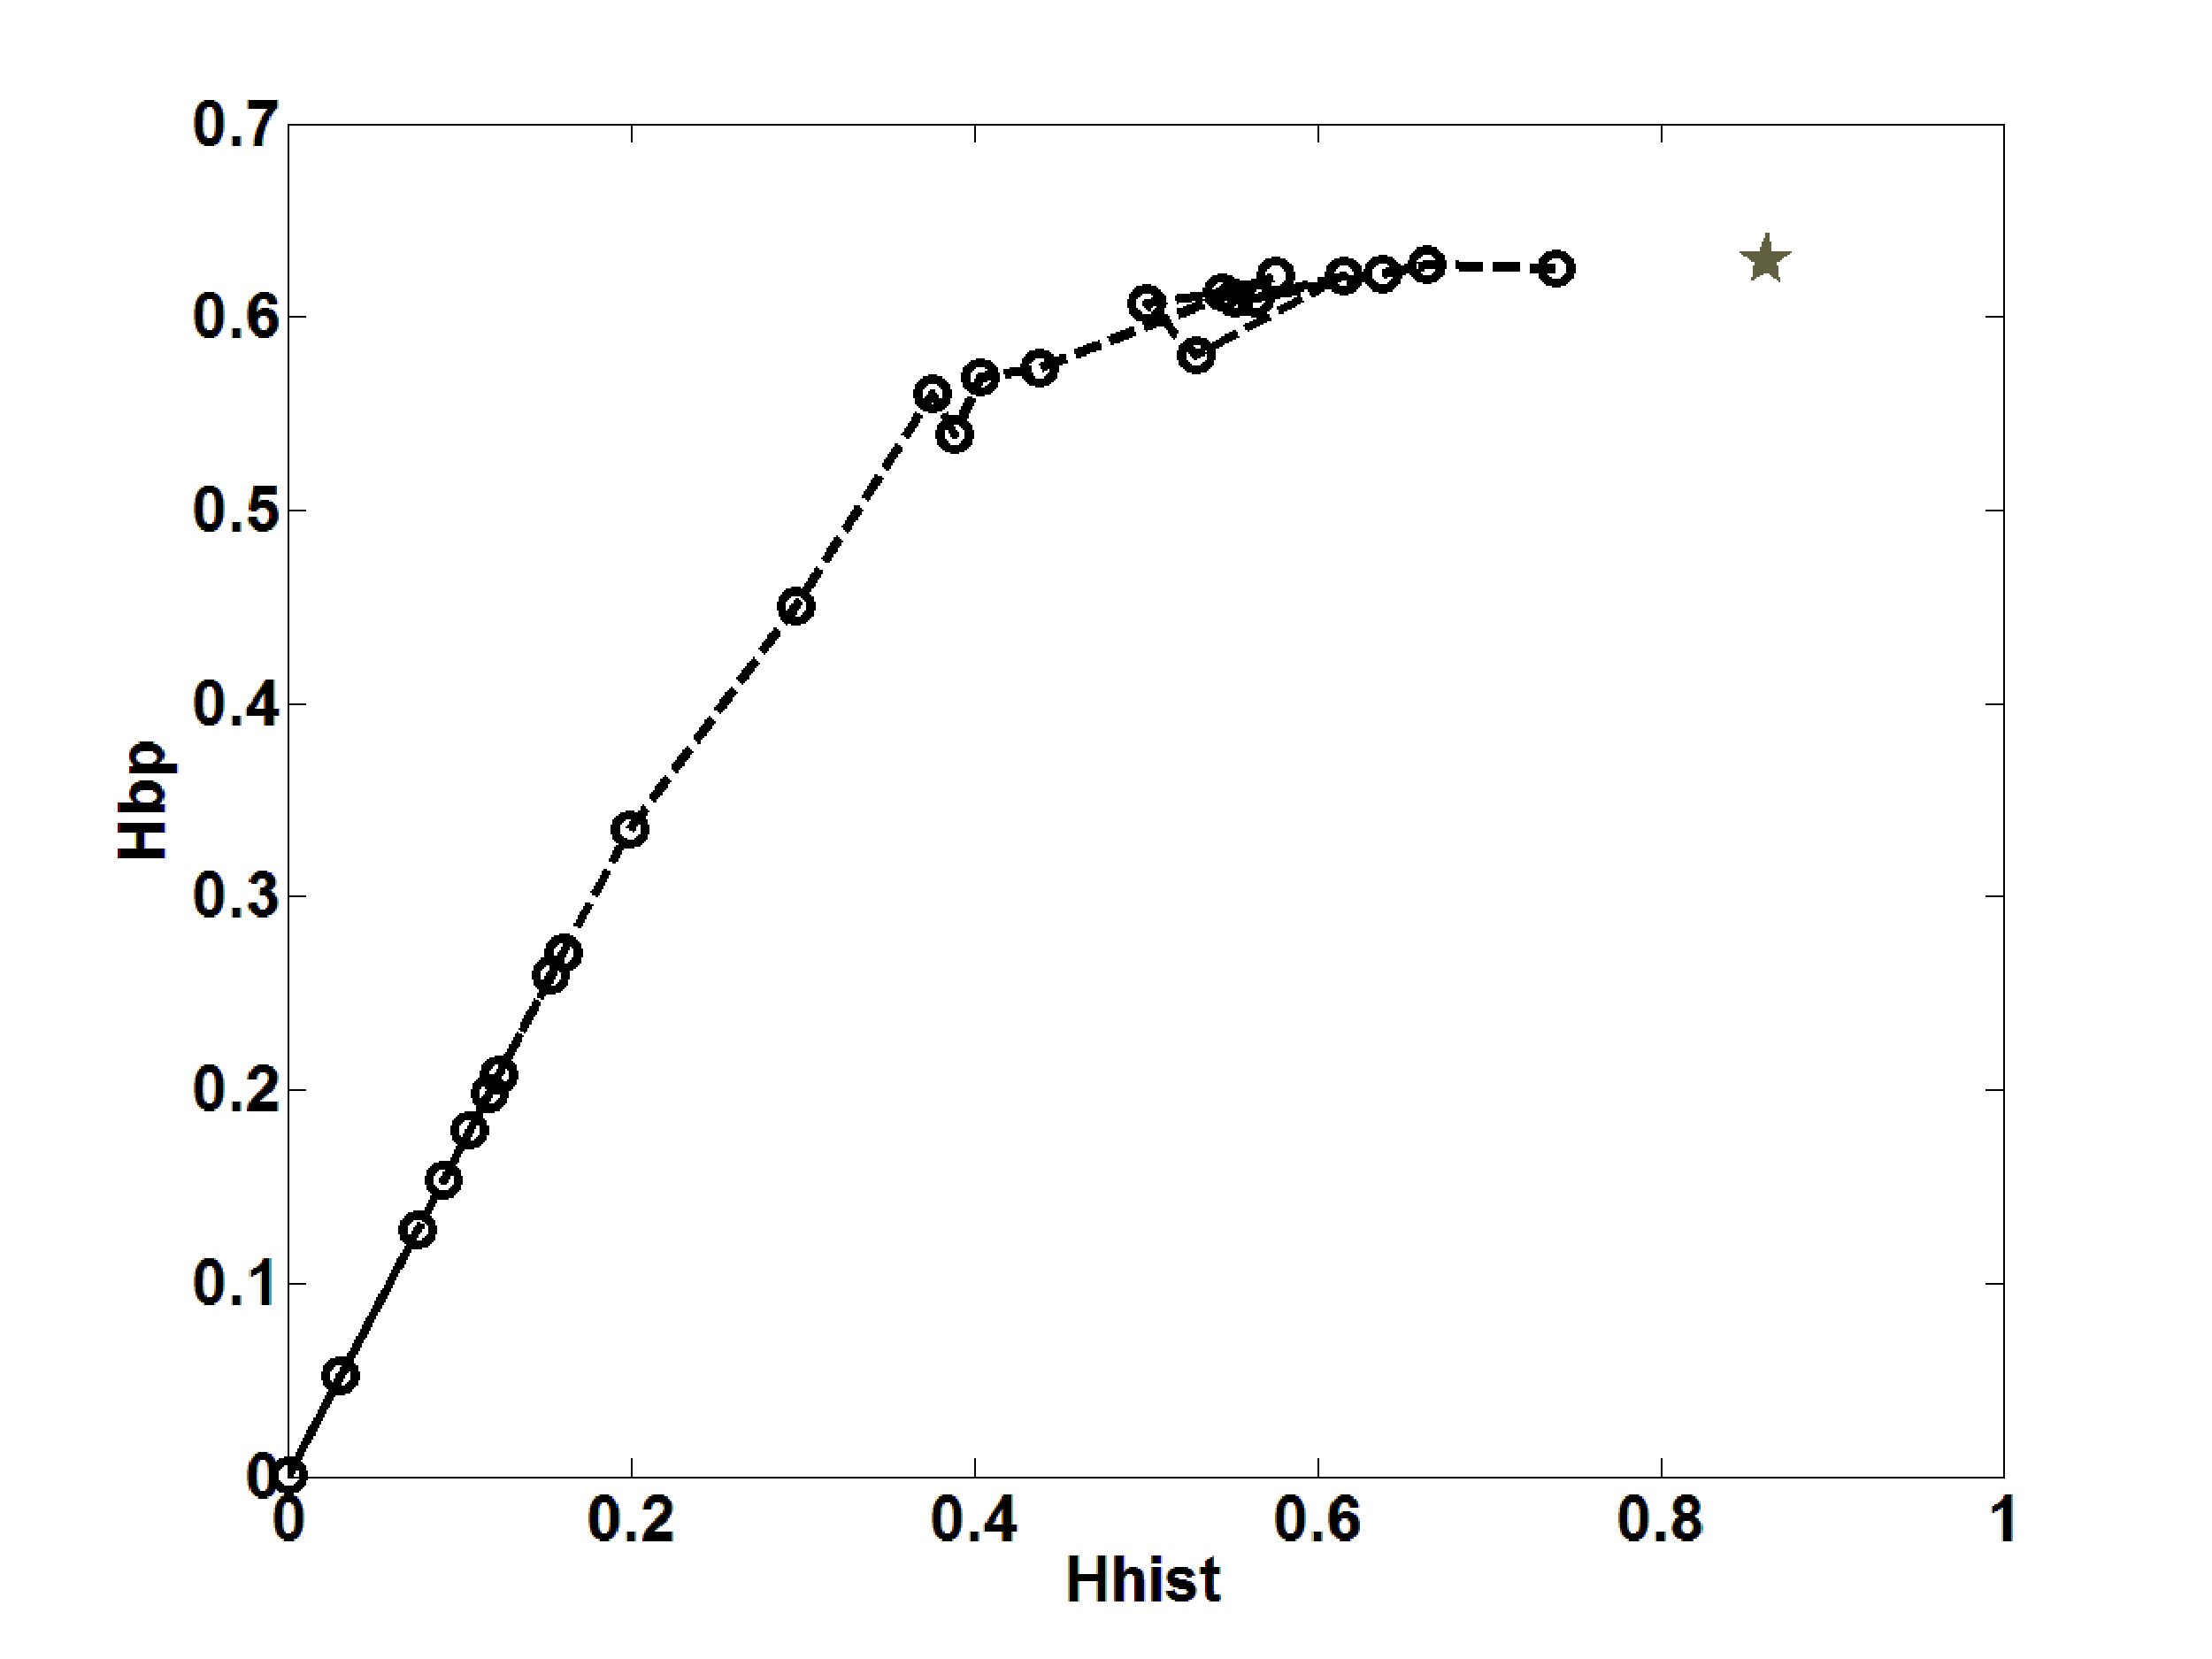
\includegraphics[width=0.3\textwidth]{HhistHbp_logisticoB2}
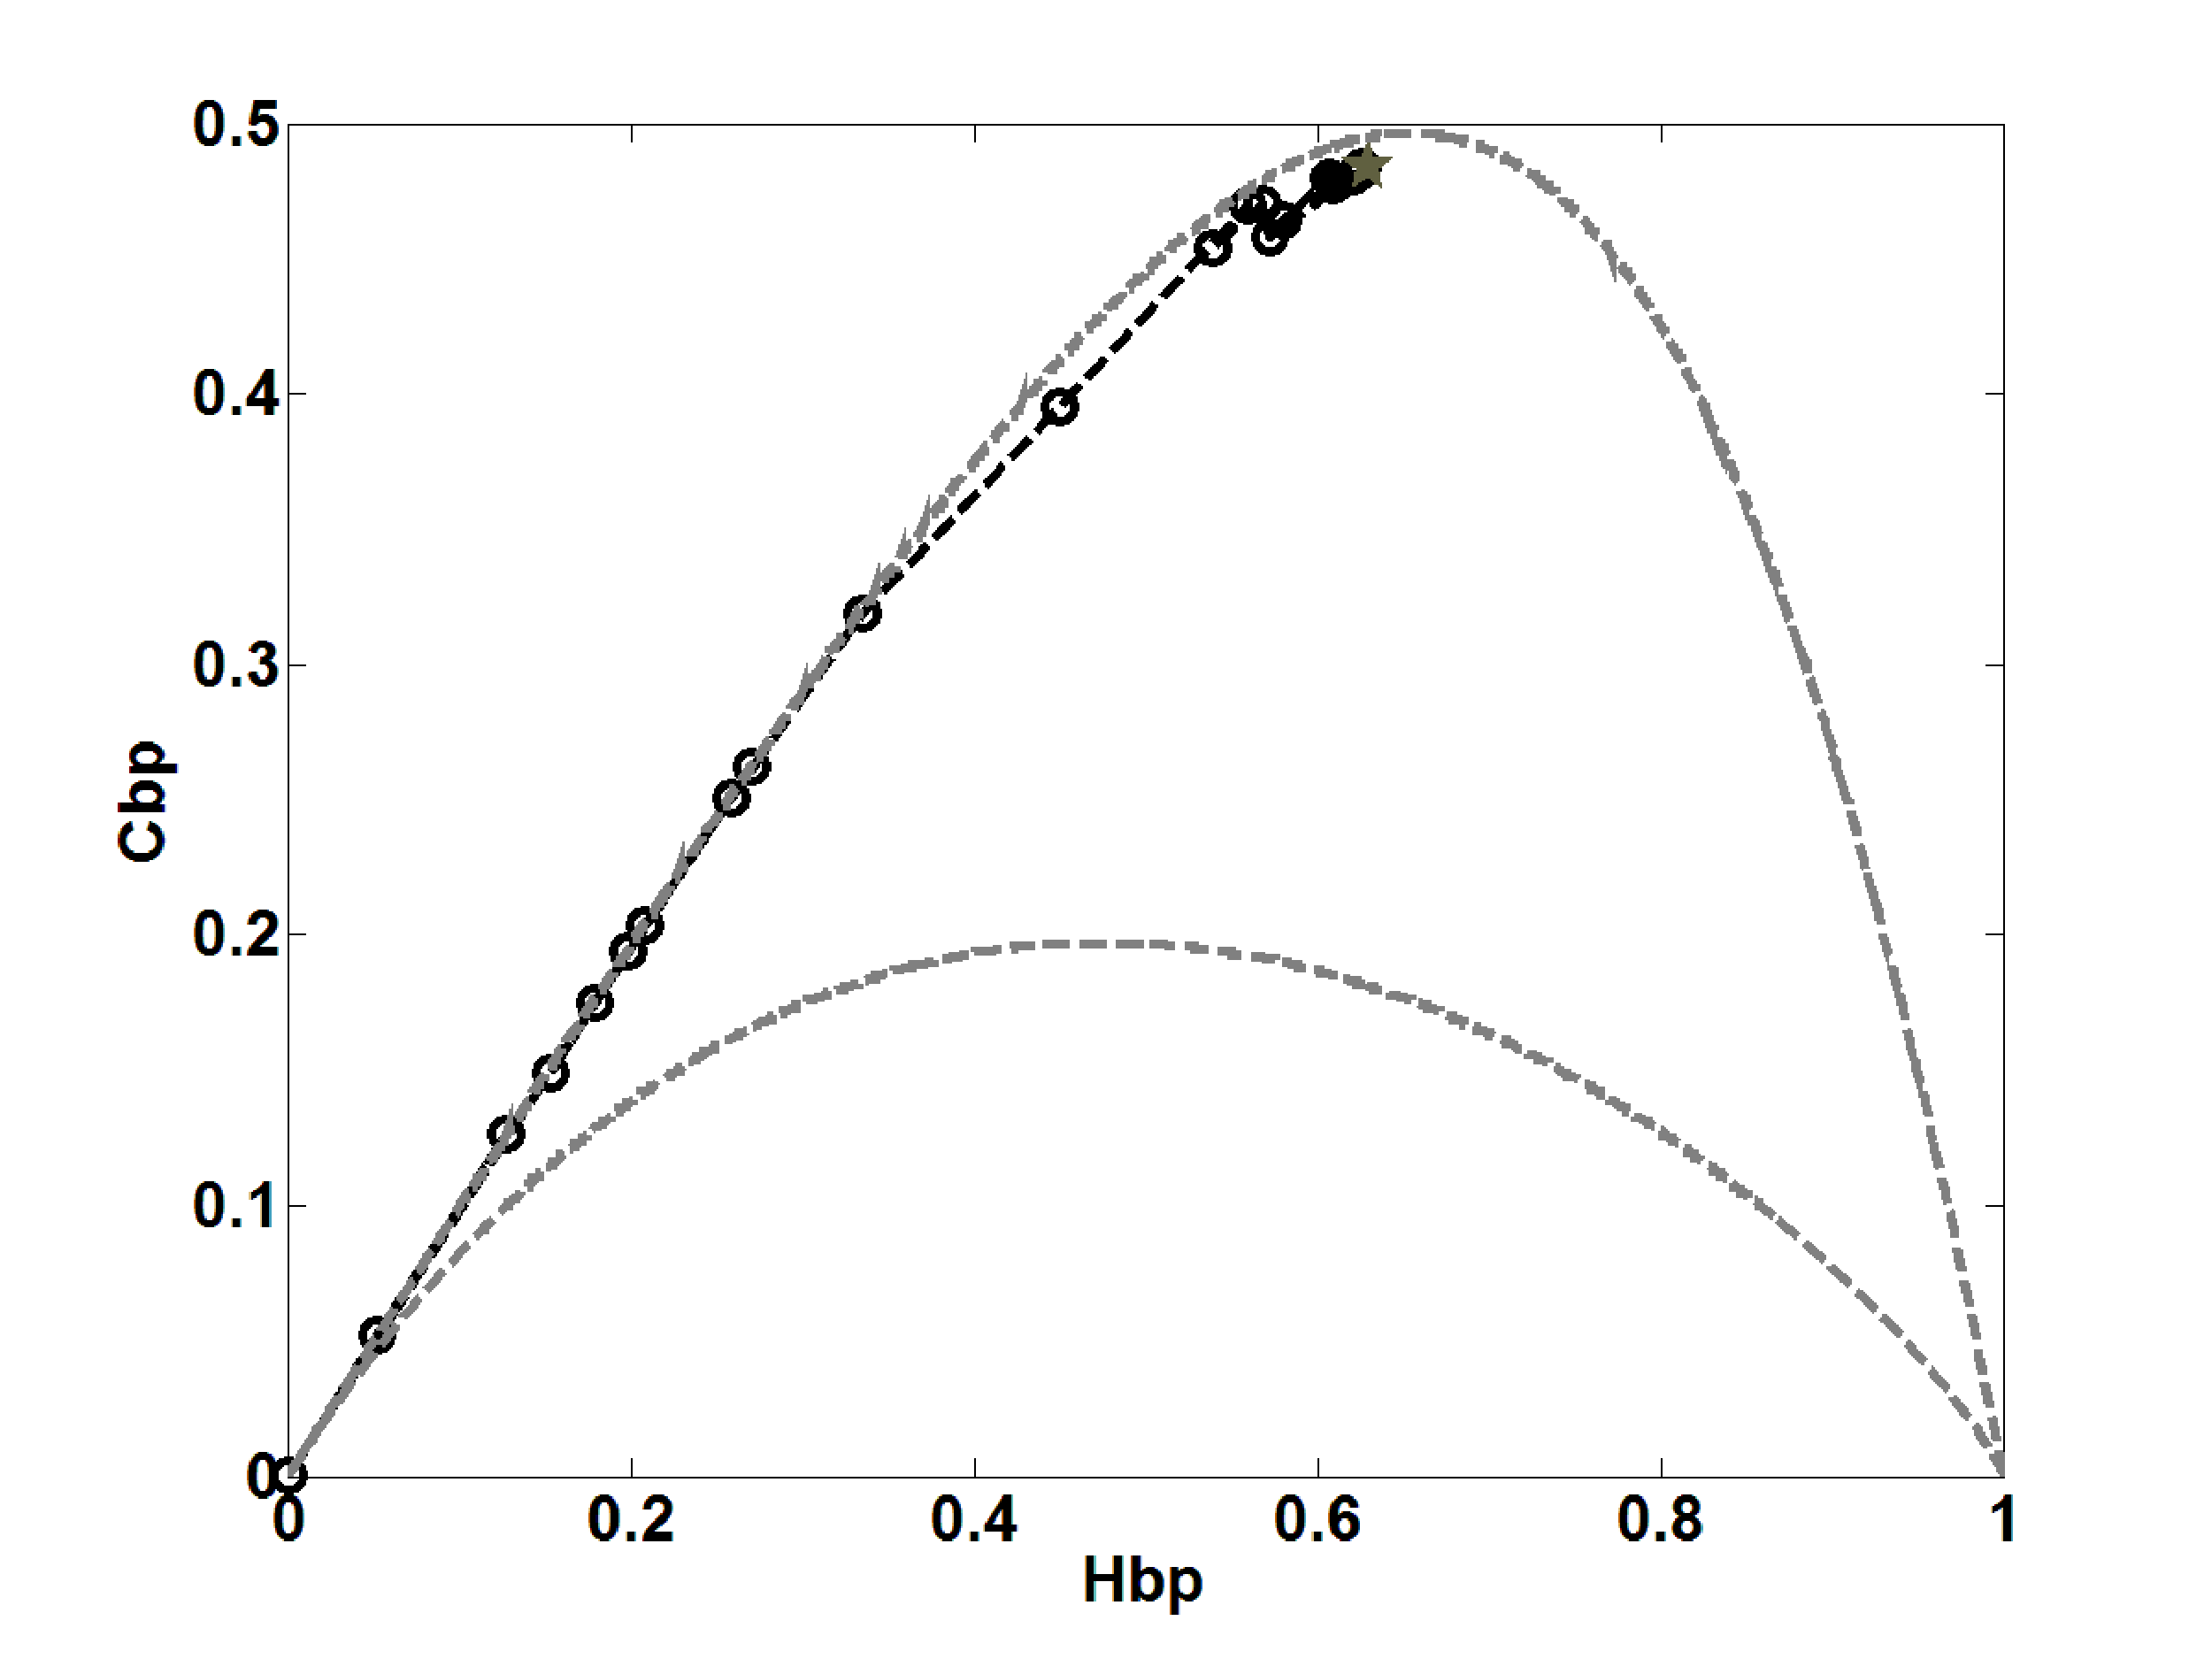
\includegraphics[width=0.3\textwidth]{HbpCbp_logisticoB2}
\caption{Statistical properties of the LOG map using binary representation: (a) $H_{hist}$ vs $P$ (b) $H_{BP}$ vs $P$ (c) $C_{BP}$ vs $P$ (d) Number of missing ordering patterns $MP$ vs $P$. In Figures (a) to (d) dashed line correspond to floating point numbers. (d) representation in the $H_{hist},H_{BP}$ plane in the the decimal numerical system.  The star represents the state for floating points numbers. (e) representation in the $H_{hist},H_{BP}$ plane. The star represents the state for floating point numbers; (f) representation in the $H_{BP},C_{BP}$ plane.  The star represents the state for floating points numbers. (f) representation in the $H_{BP},C_{BP}$ plane for binary numerical system.  The star represents the state for floating points numbers. } \label{fig:LOGbinario}
\end{figure}

%%%%%%%%%%%%%%%%%%%%%%%%%%
%%%%%%%%%%%%%%%%%%%%%%%%%%% Fig.5
\begin{figure}
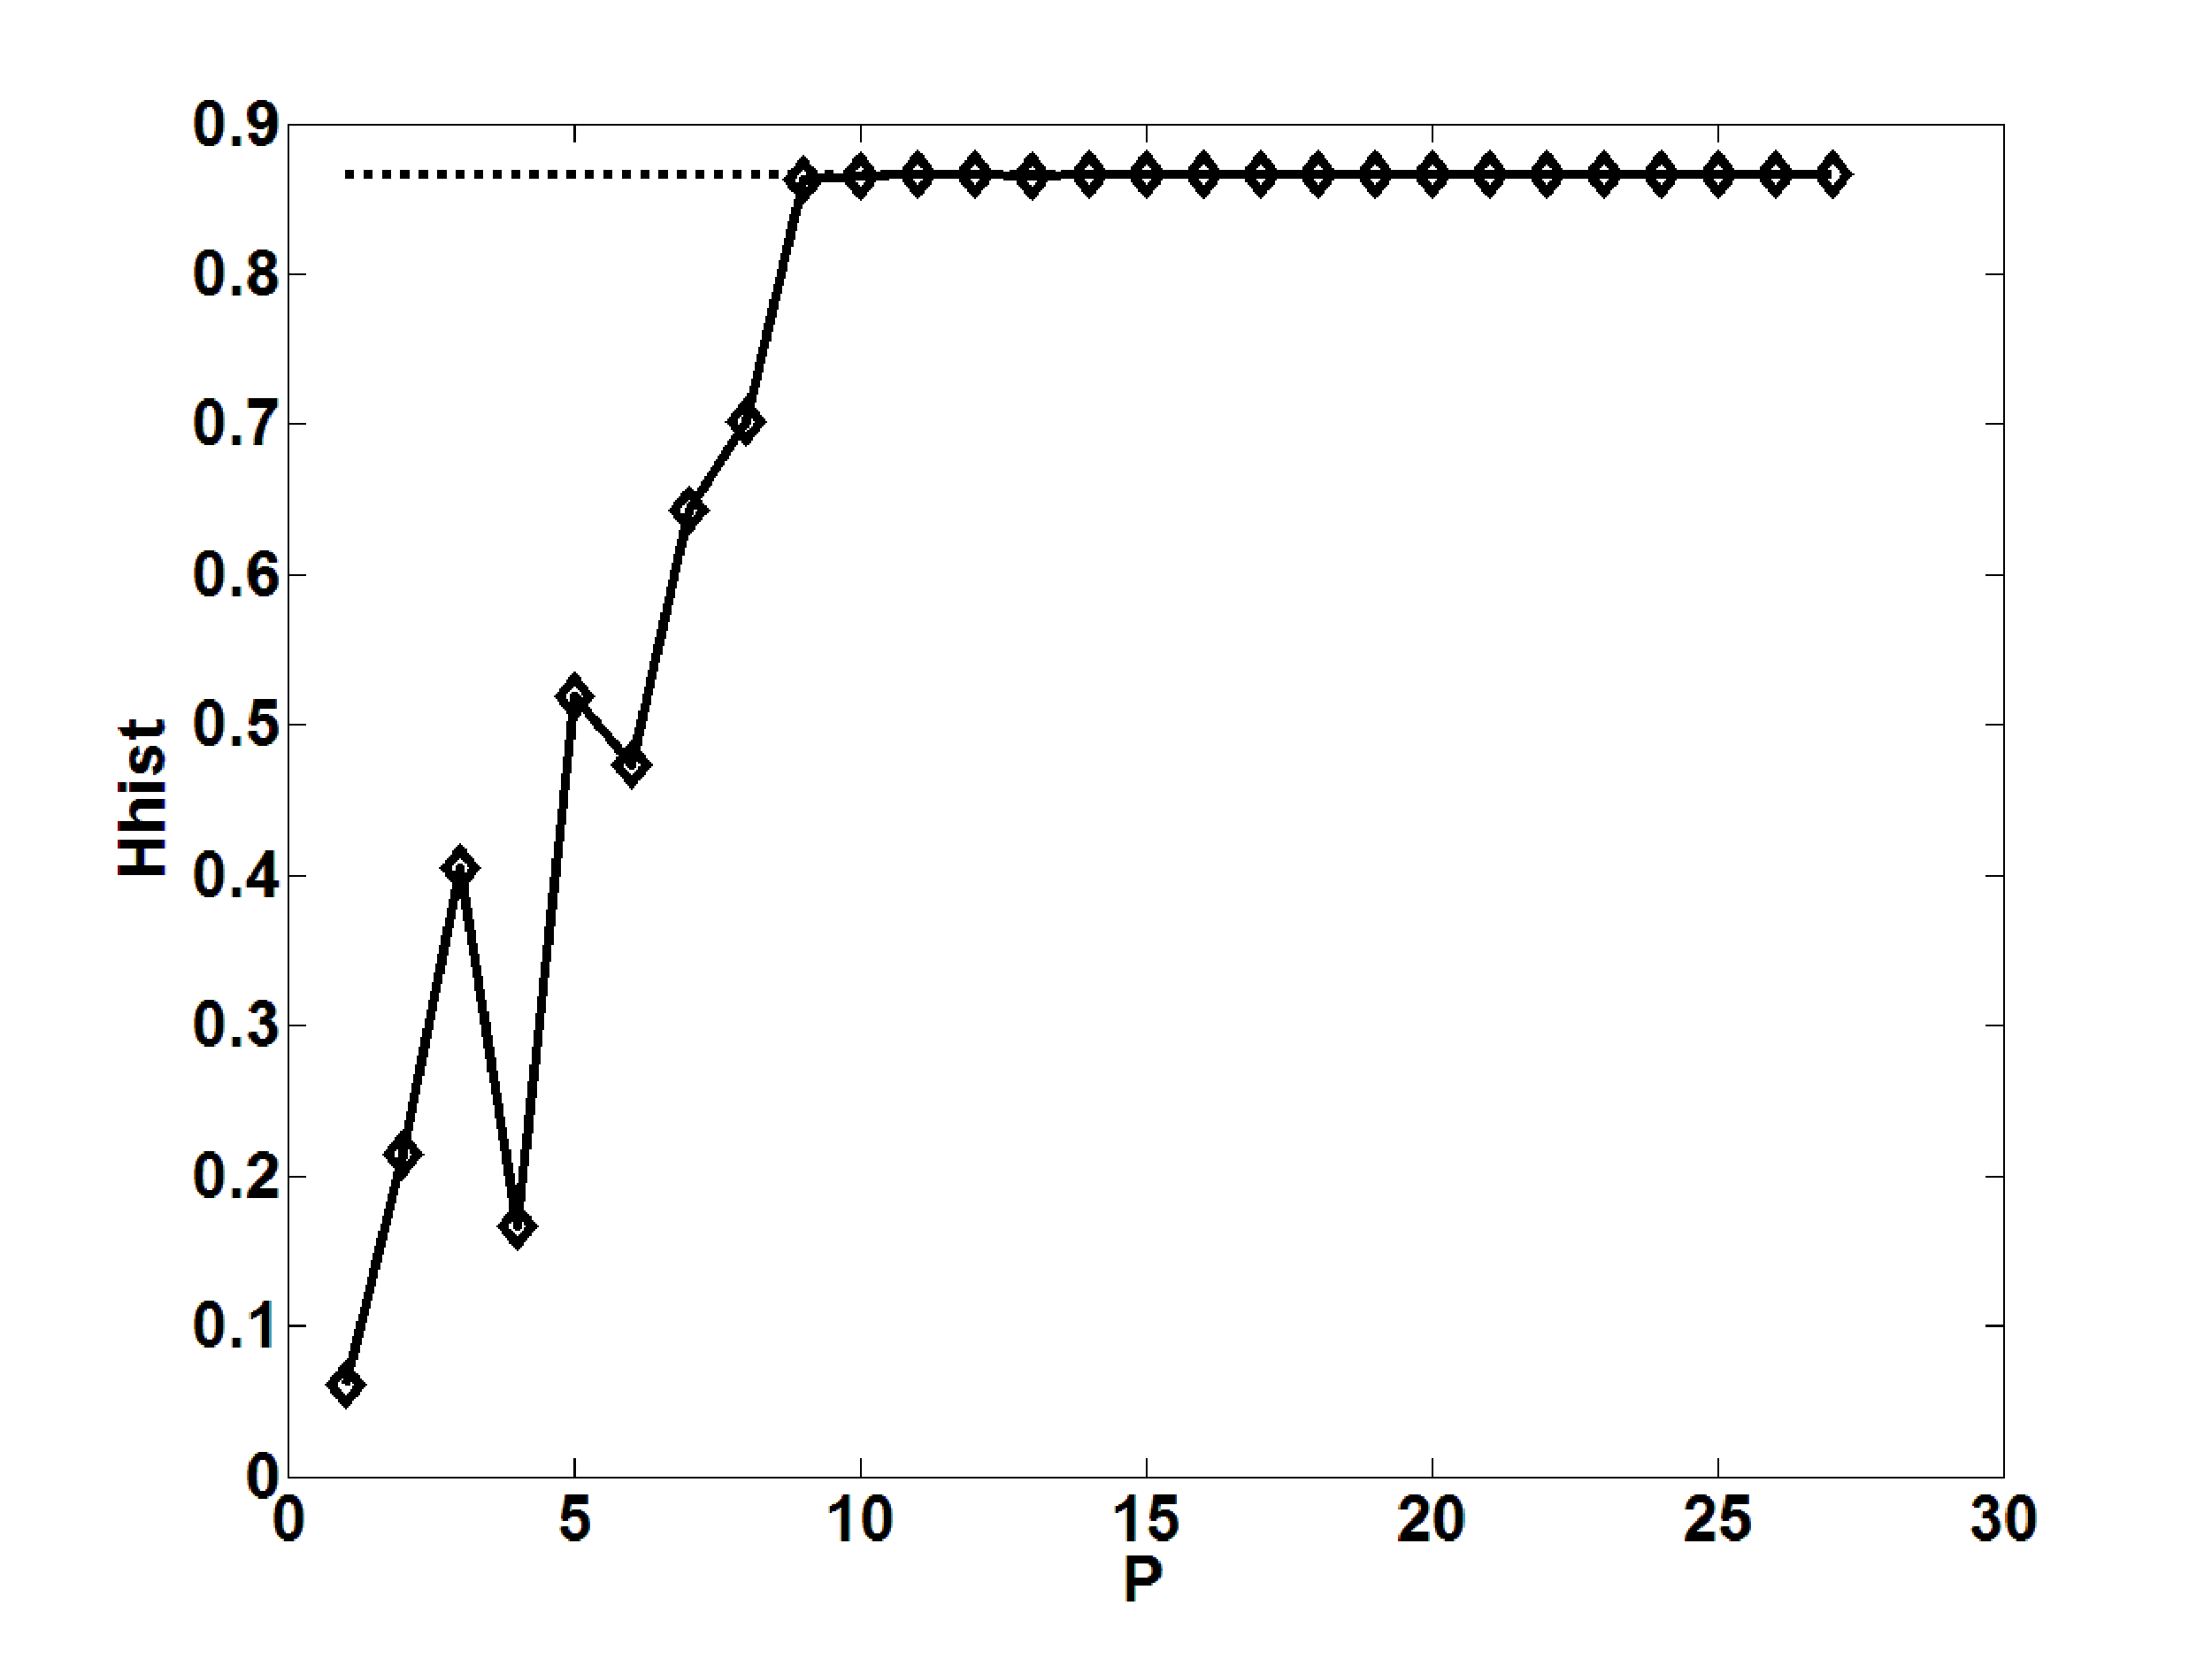
\includegraphics[width=0.3\textwidth]{Hhist_switchB10}
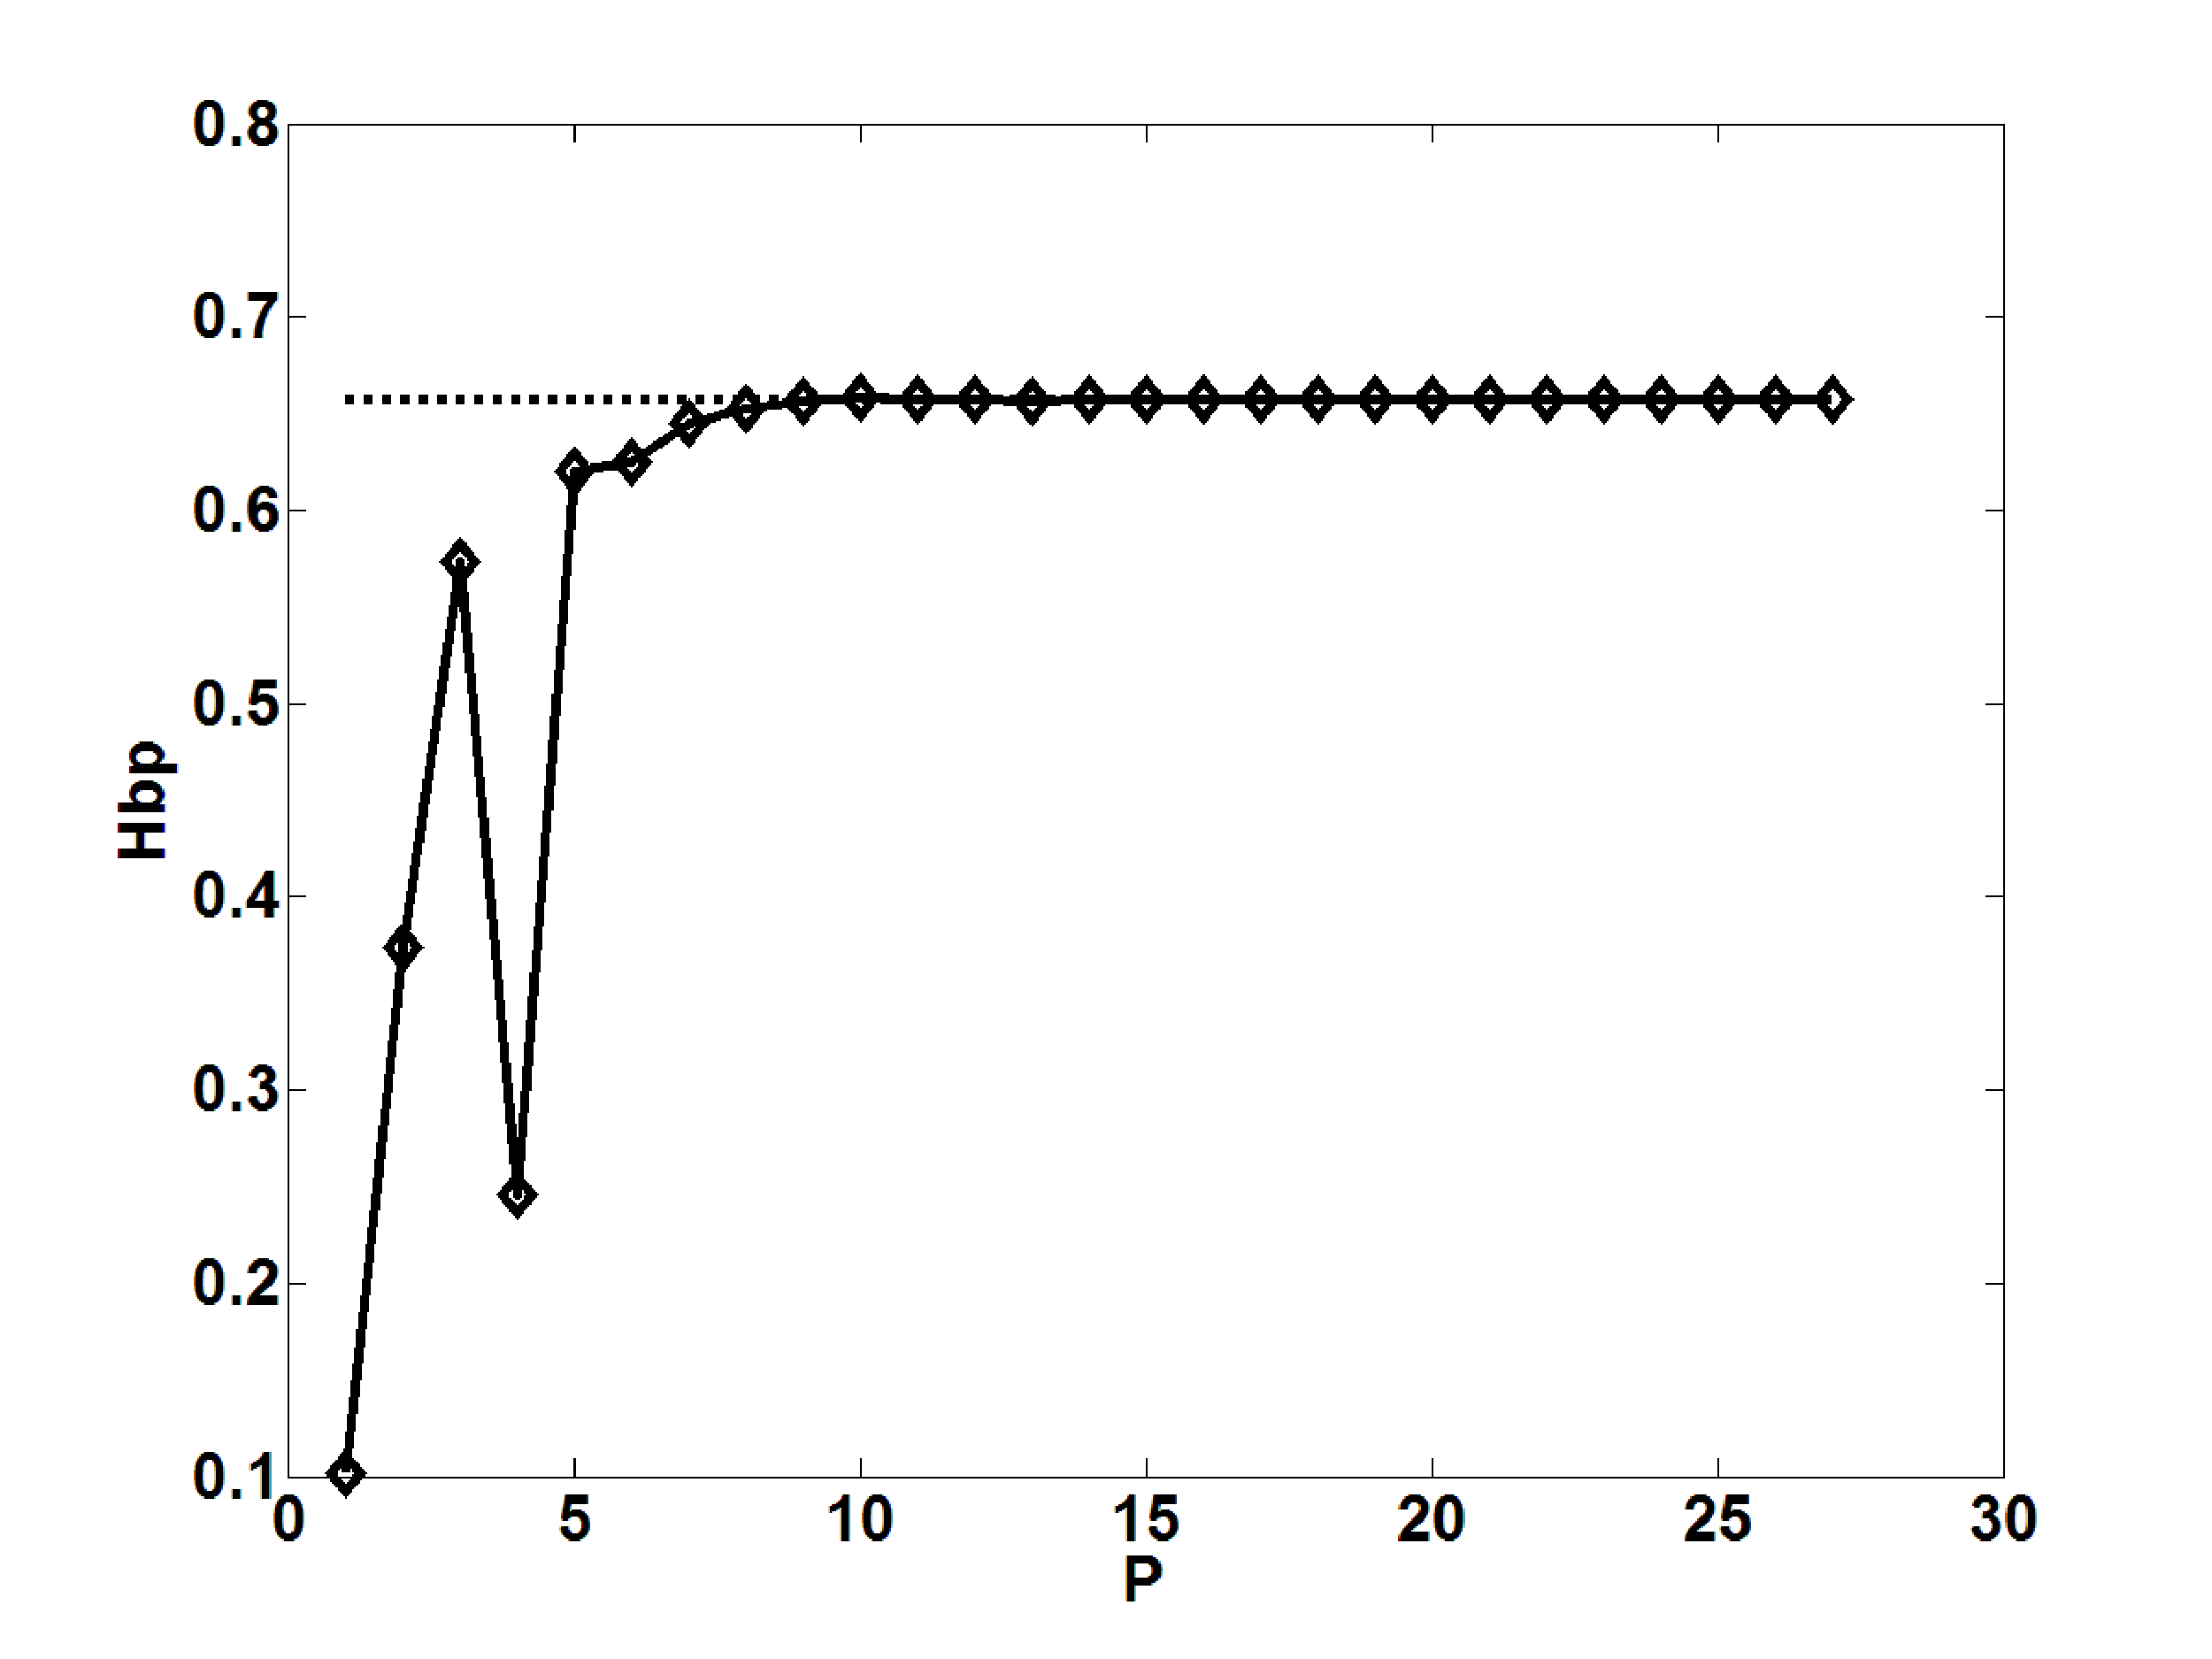
\includegraphics[width=0.3\textwidth]{Hbp_switchB10}
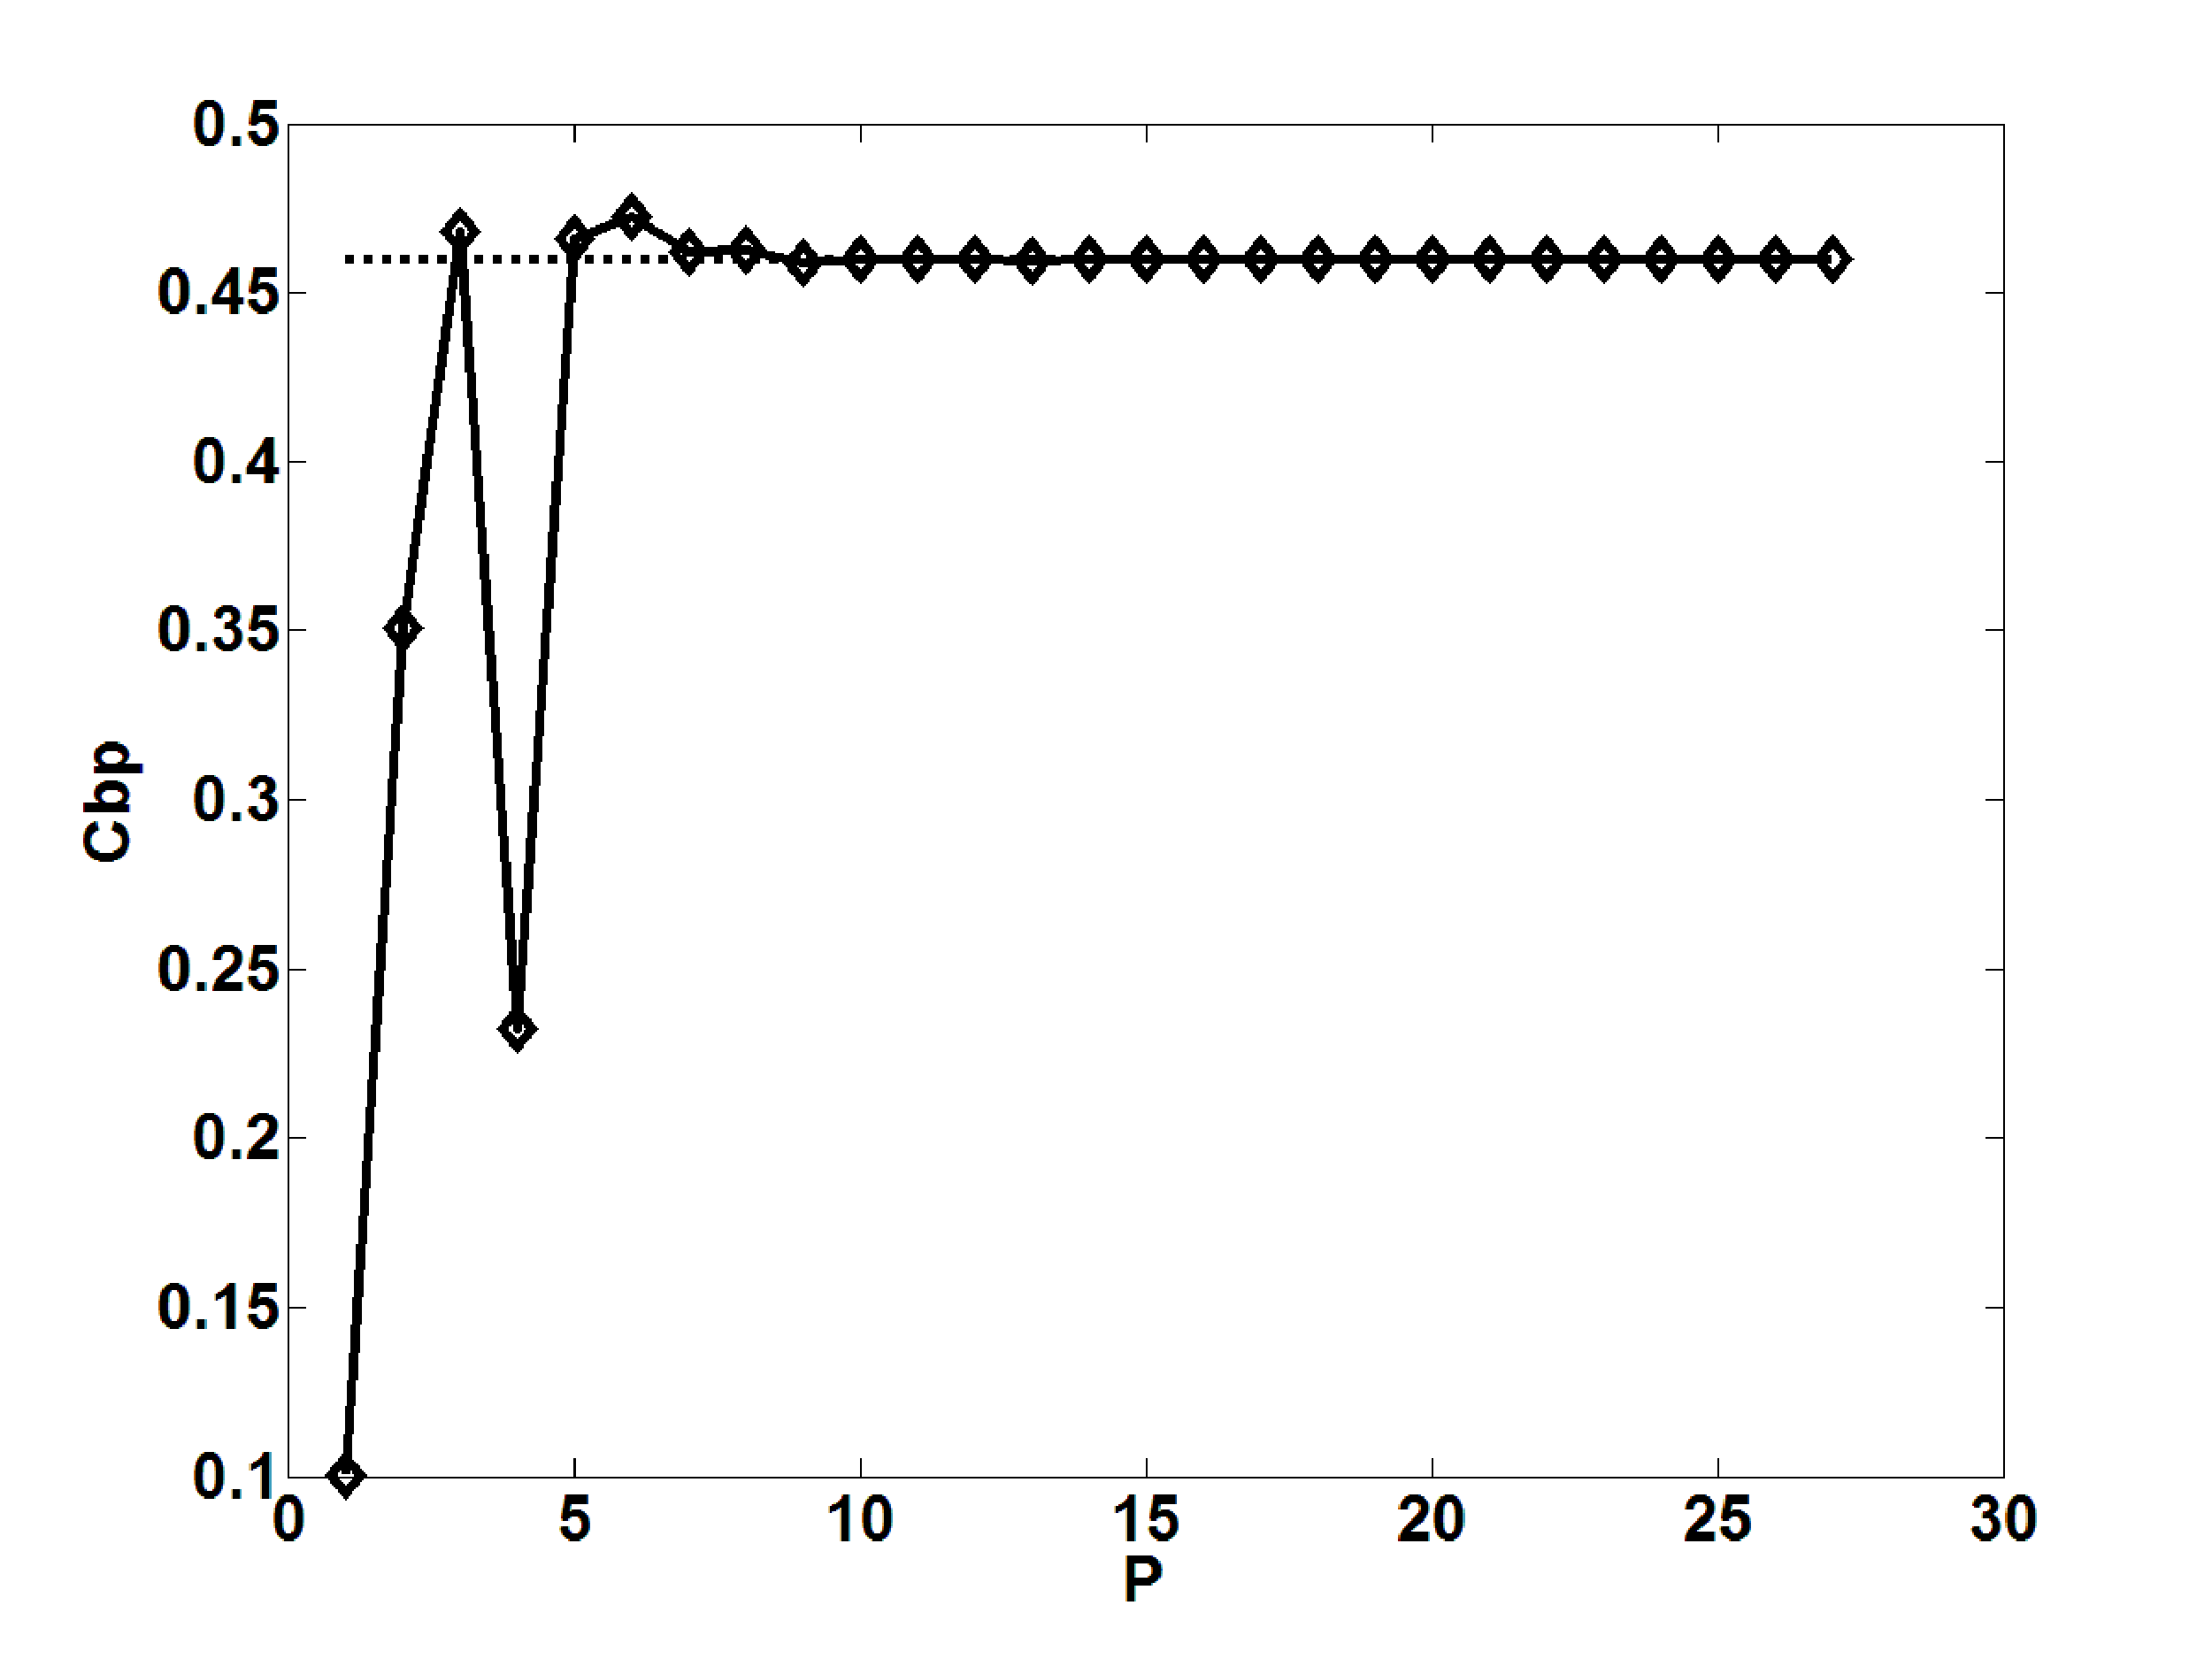
\includegraphics[width=0.3\textwidth]{Cbp_switchB10}
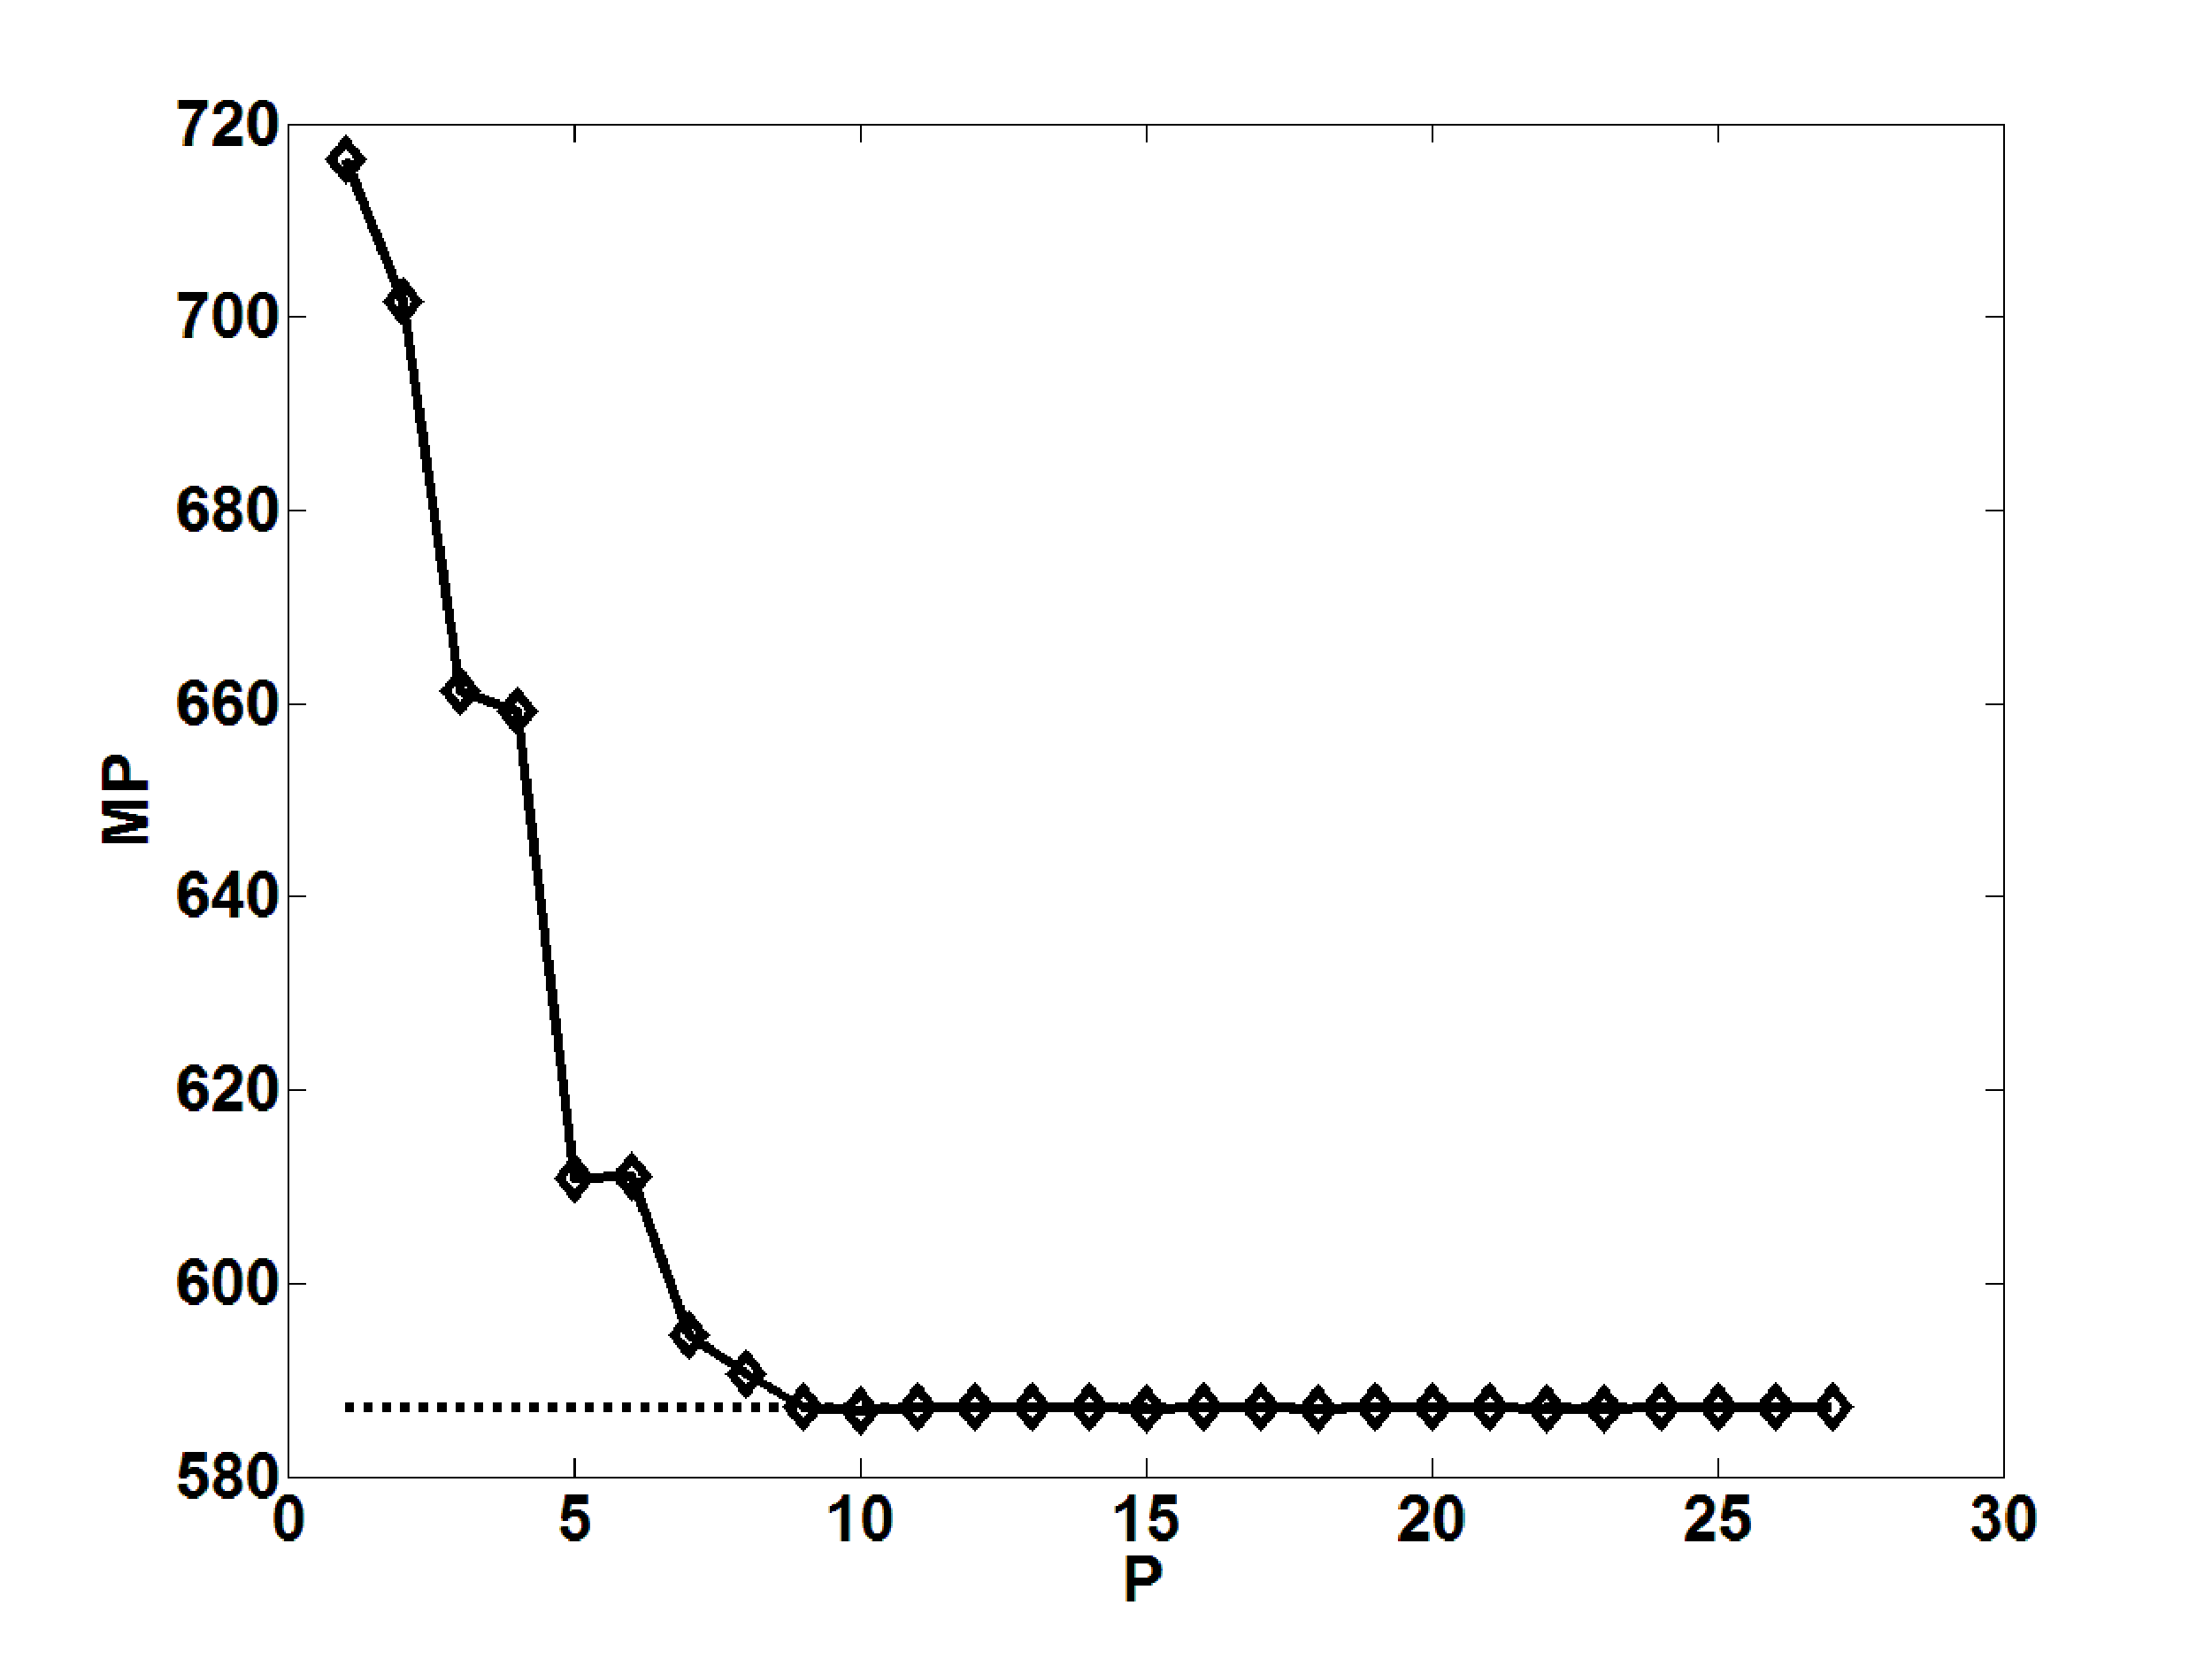
\includegraphics[width=0.3\textwidth]{Miss_switchB10}
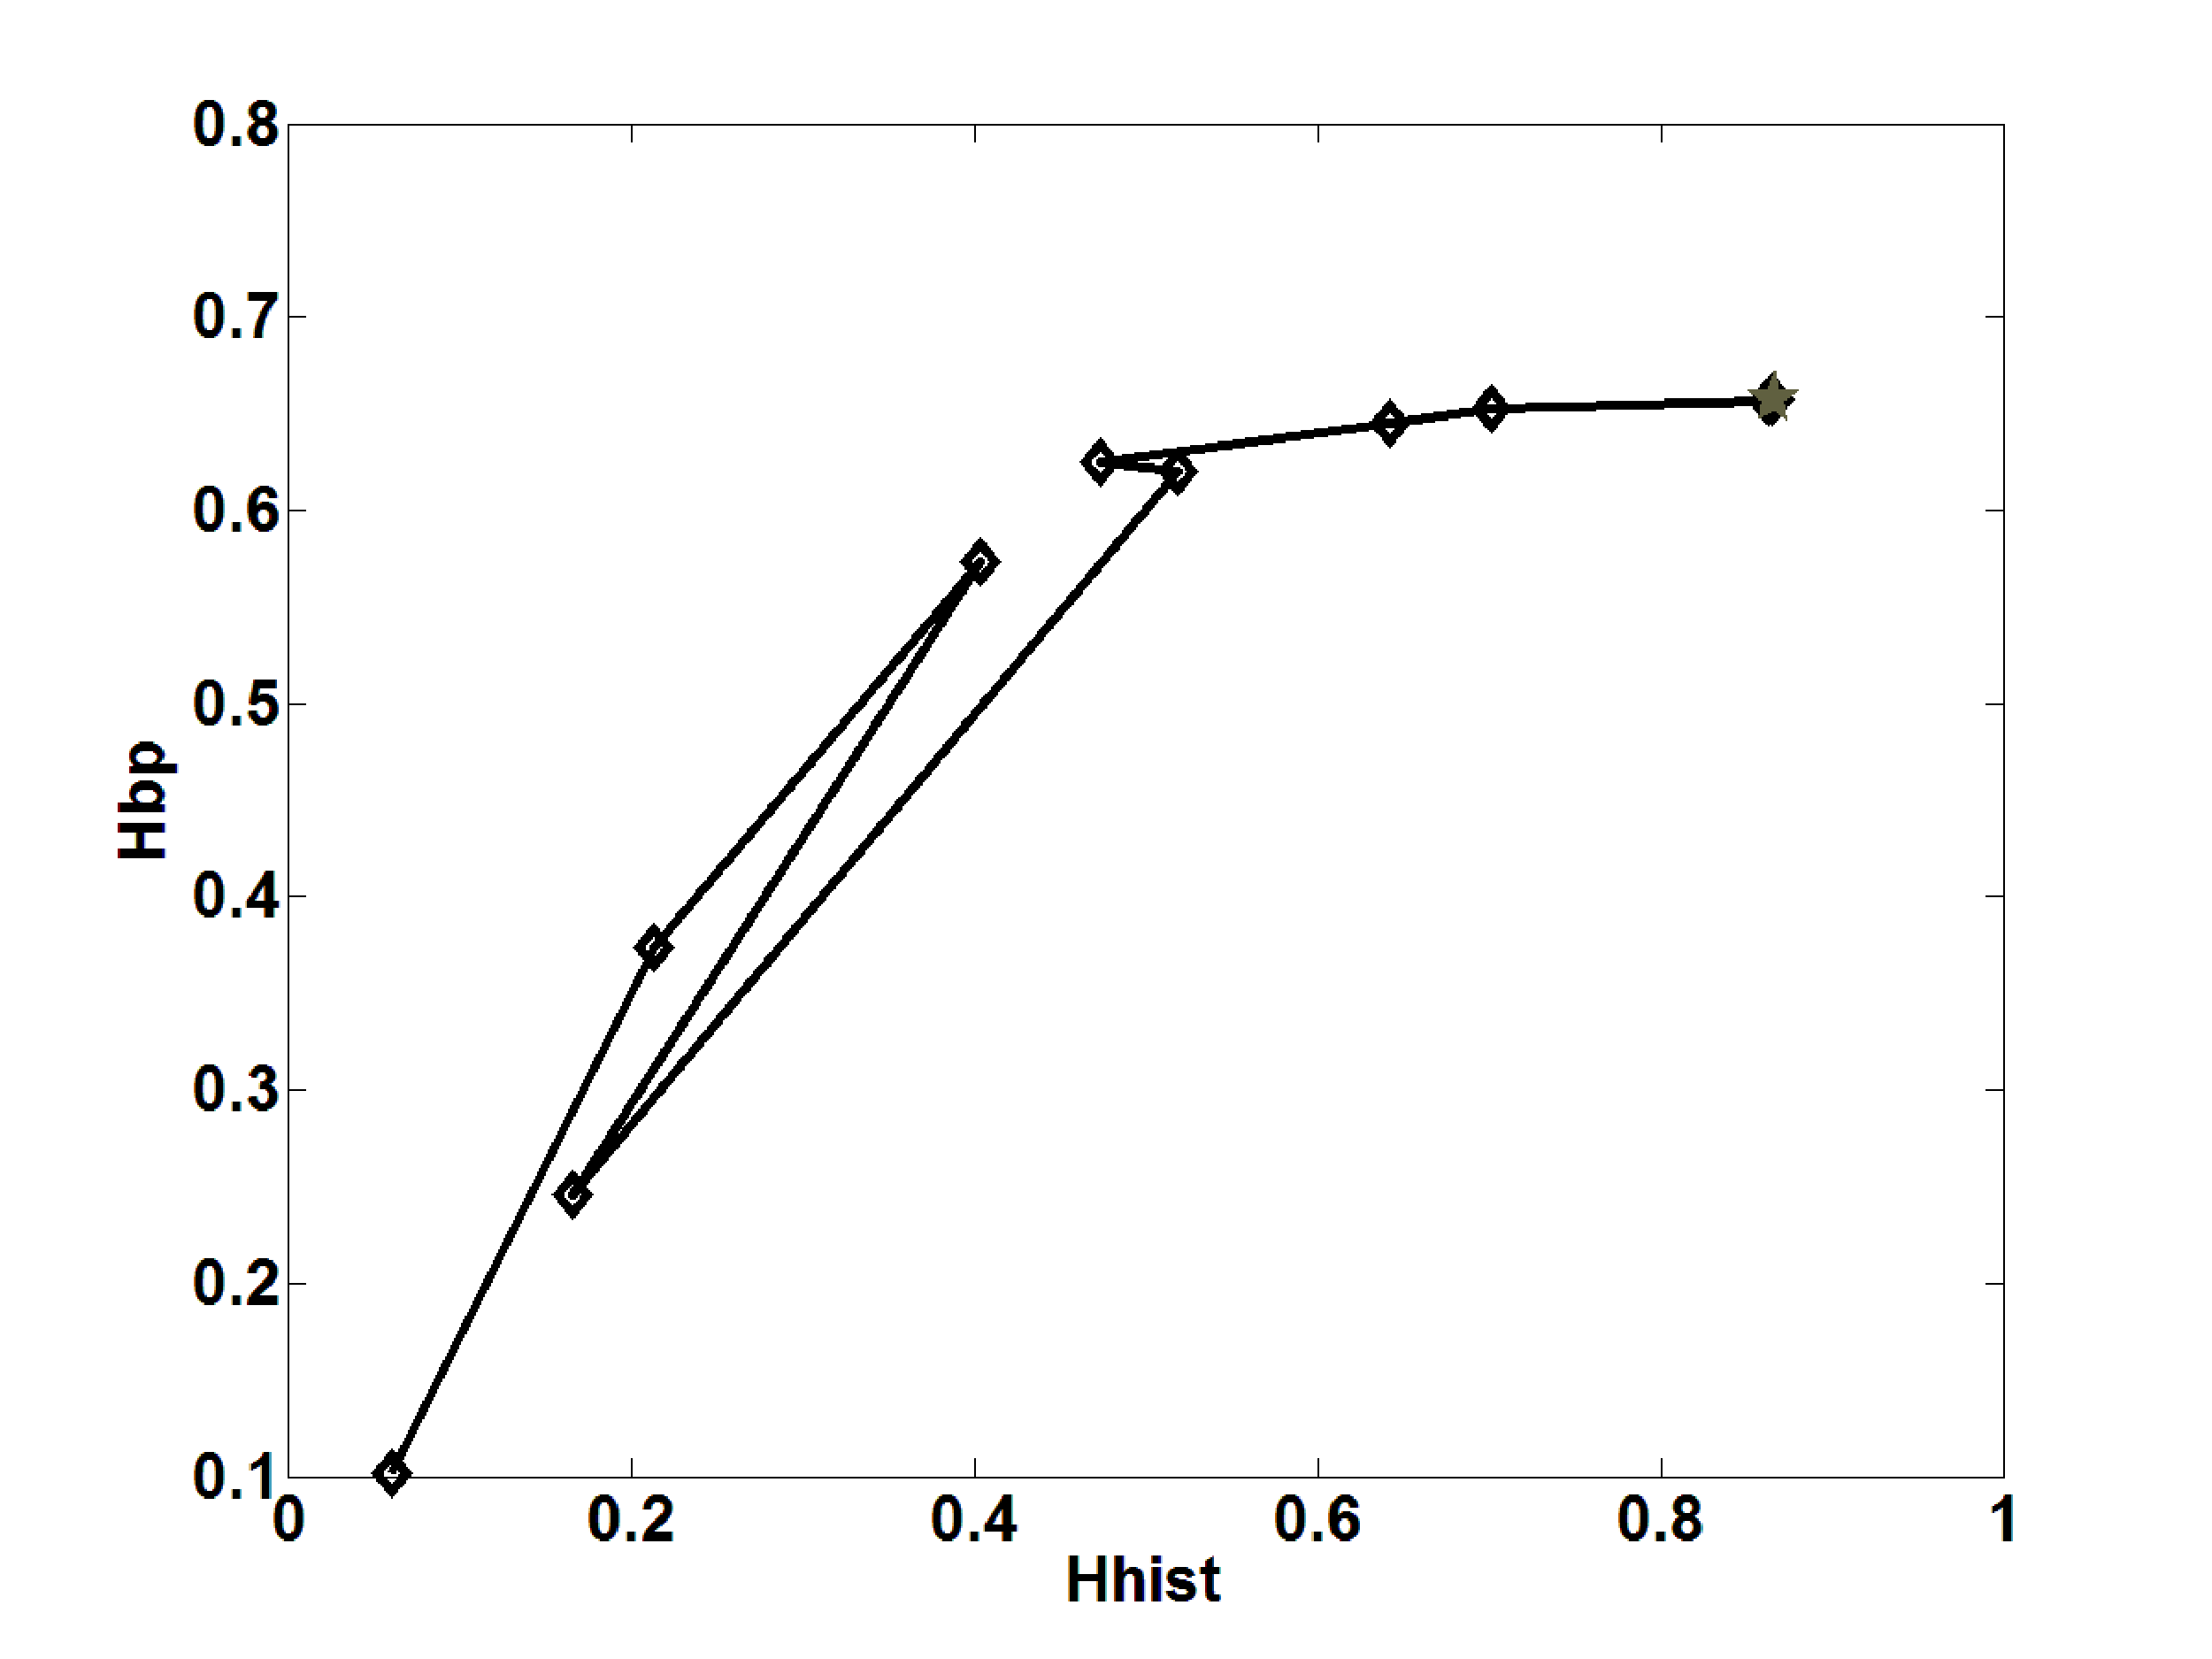
\includegraphics[width=0.3\textwidth]{HhistHbp_switchB10}
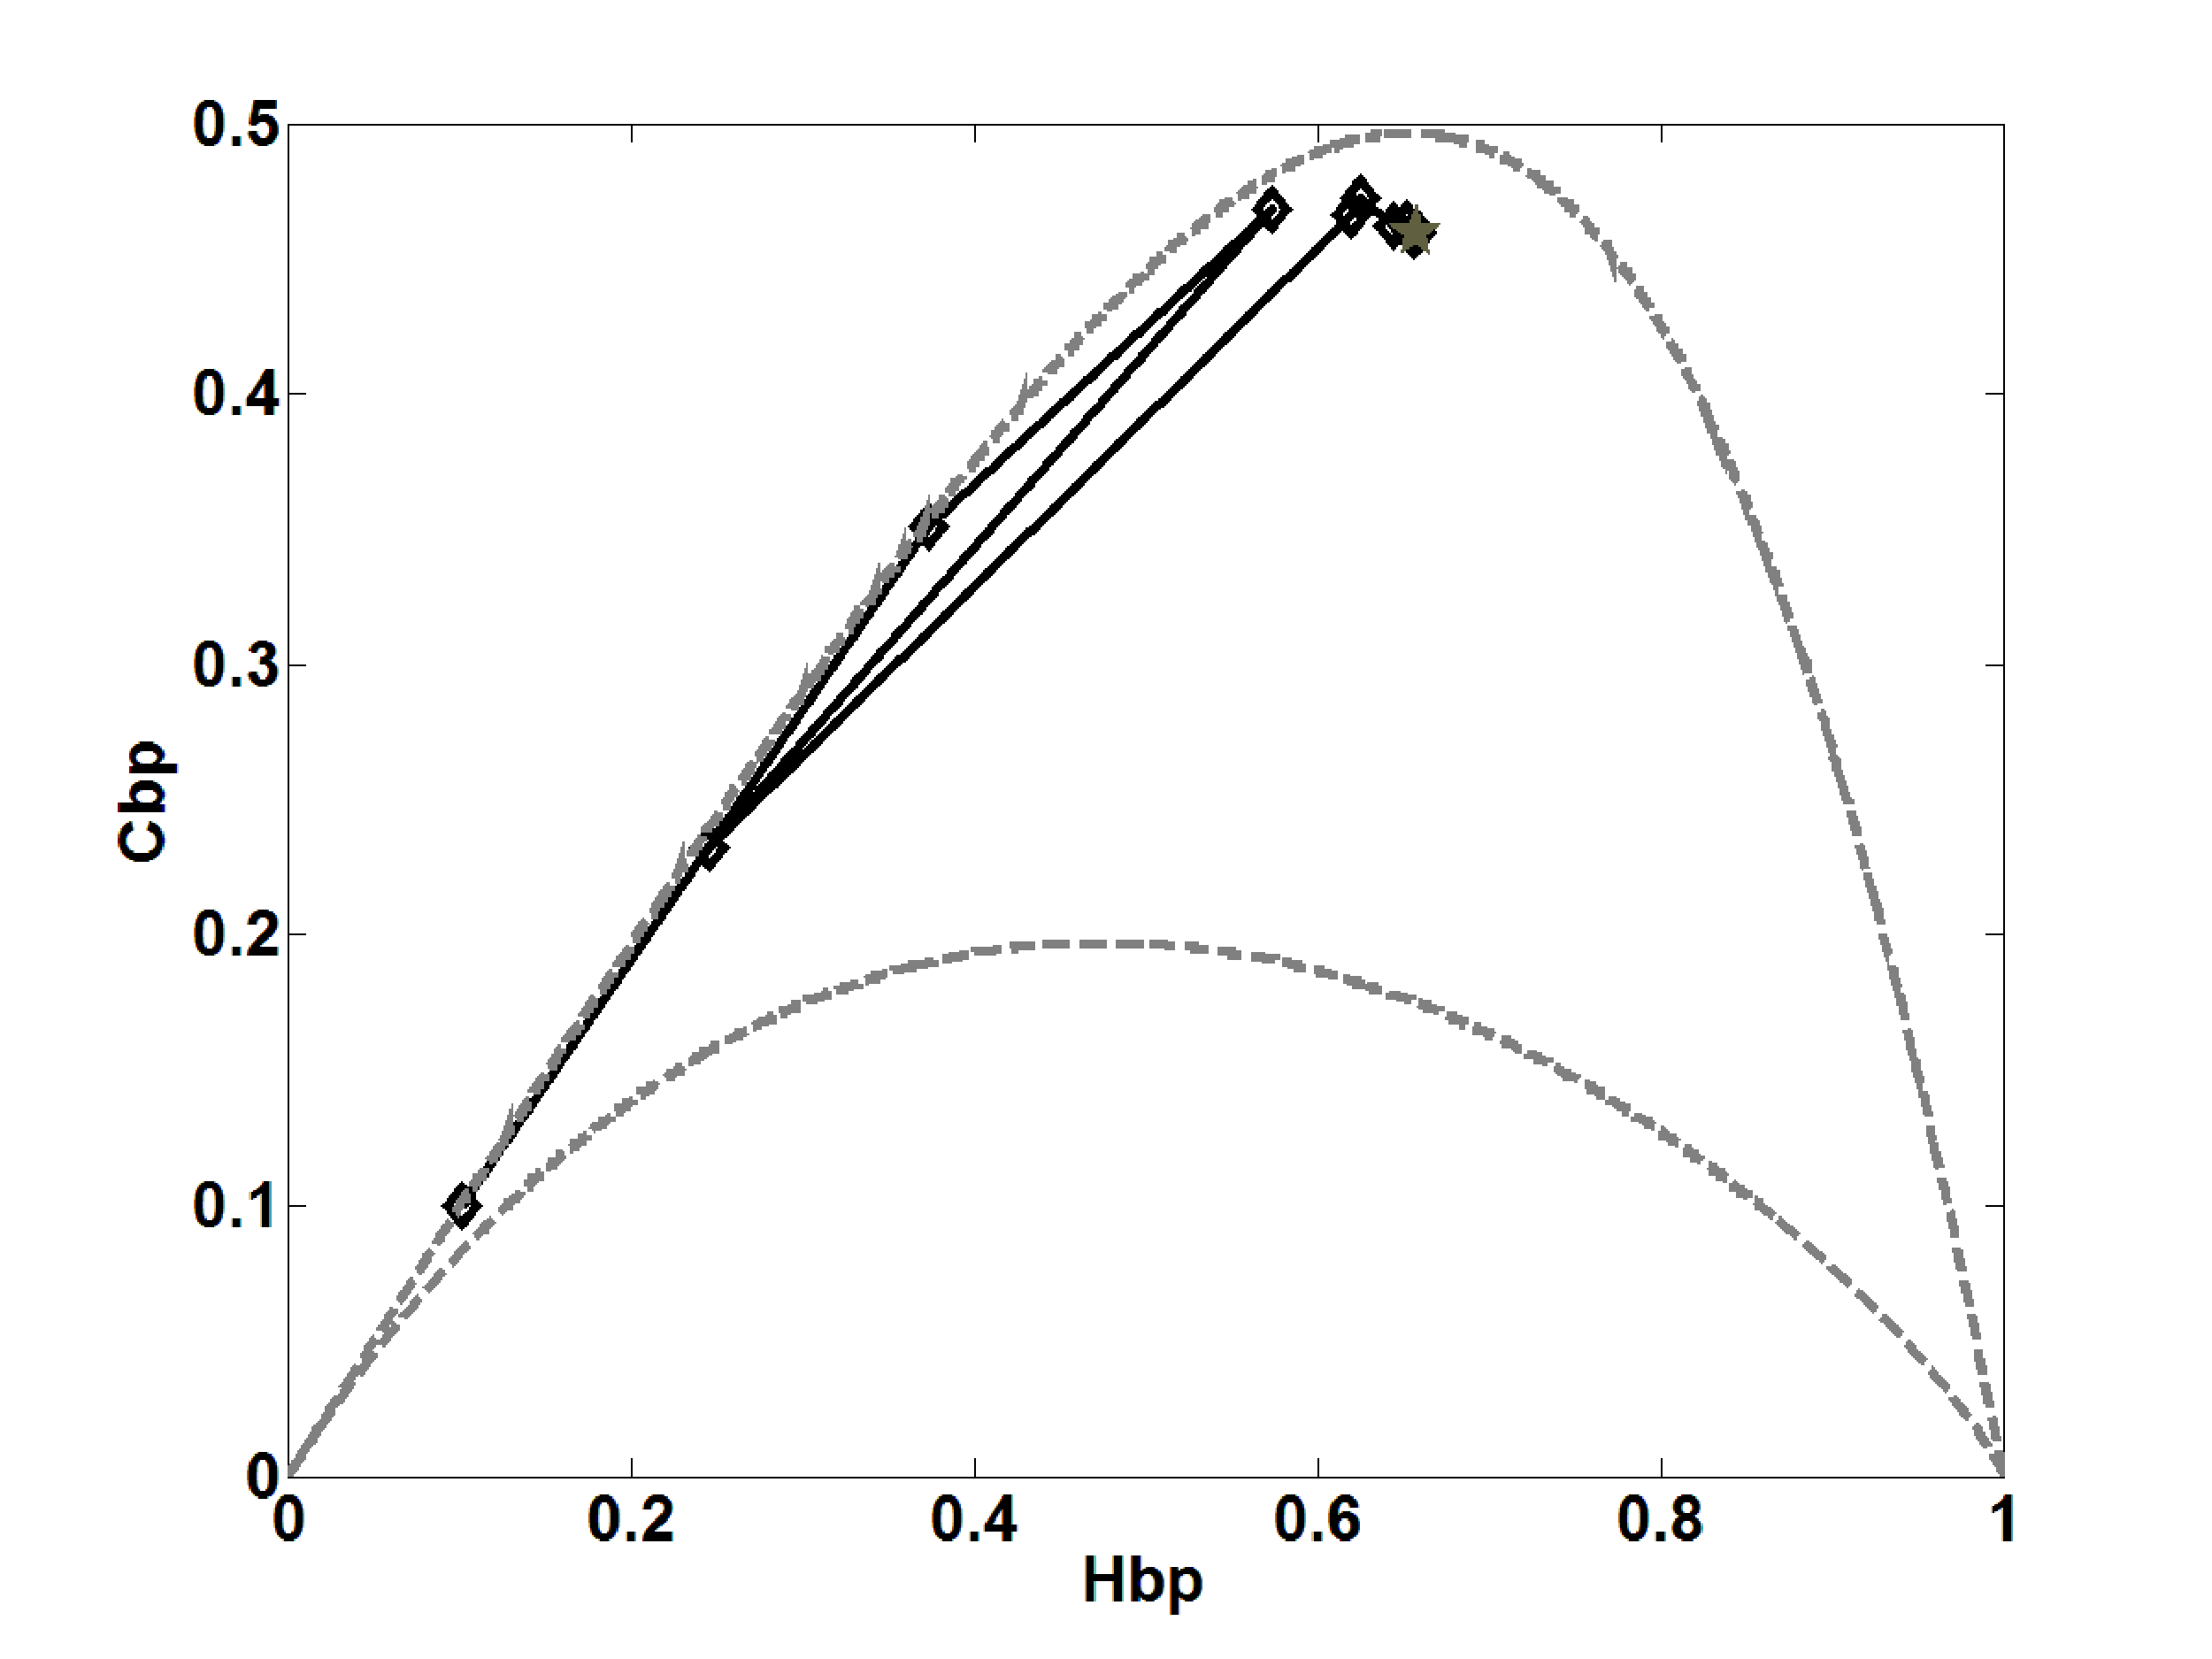
\includegraphics[width=0.3\textwidth]{HbpCbp_switchB10}
\caption{Statistical properties of the SWITCH map using decimal representation: (a) $H_{hist}$ vs $P$ (b) $H_{BP}$ vs $P$ (c) $C_{BP}$ vs $P$ (d) Number of missing ordering patterns $MP$ vs $P$. In Figures (a) to (d) dashed line correspond to floating point numbers. (e) representation in the $H_{hist},H_{BP}$ plane in the the decimal numerical system.  The star represents the state for floating points numbers. (f) representation in the $H_{BP},C_{BP}$ plane.  The star represents the state for floating points numbers. (The star represents the state for floating points numbers). } \label{fig:seqdec}
\end{figure}

%%%%%%%%%%%%%%%%%%%%%%%%%%
%%%%%%%%%%%%%%%%%%%%%%%%%%% Fig.6
\begin{figure}
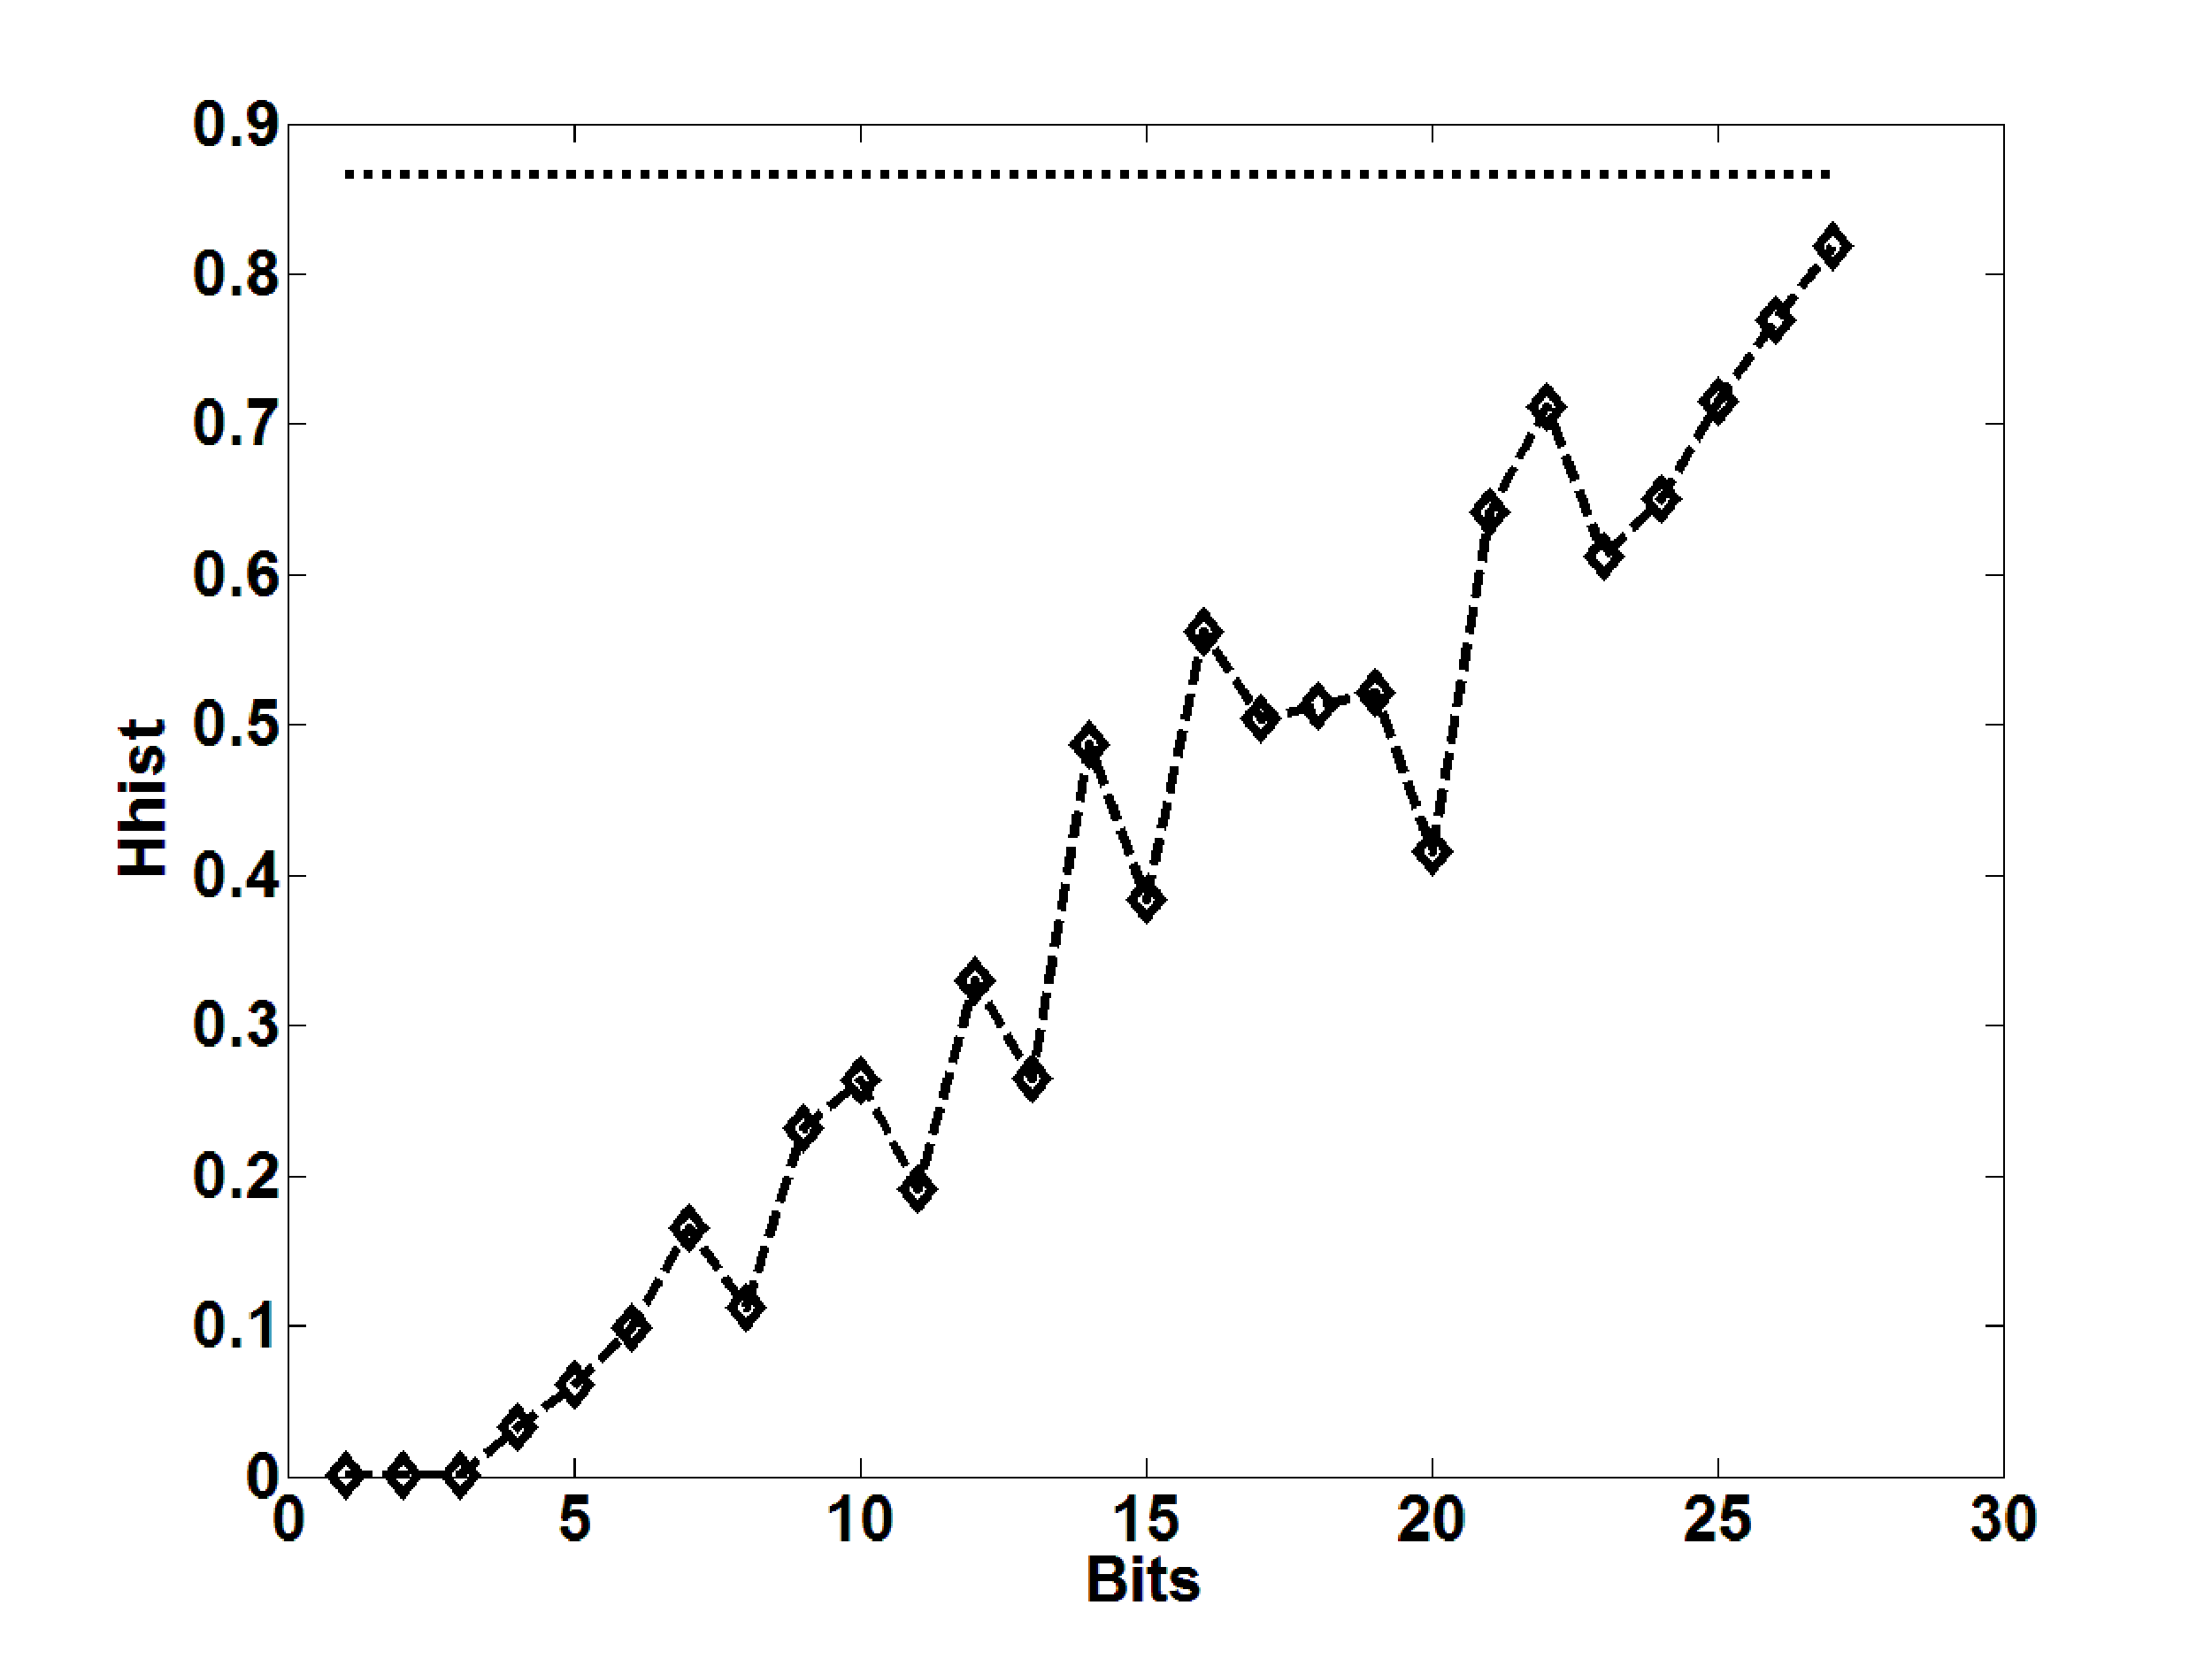
\includegraphics[width=0.3\textwidth]{Hhist_switchB2}
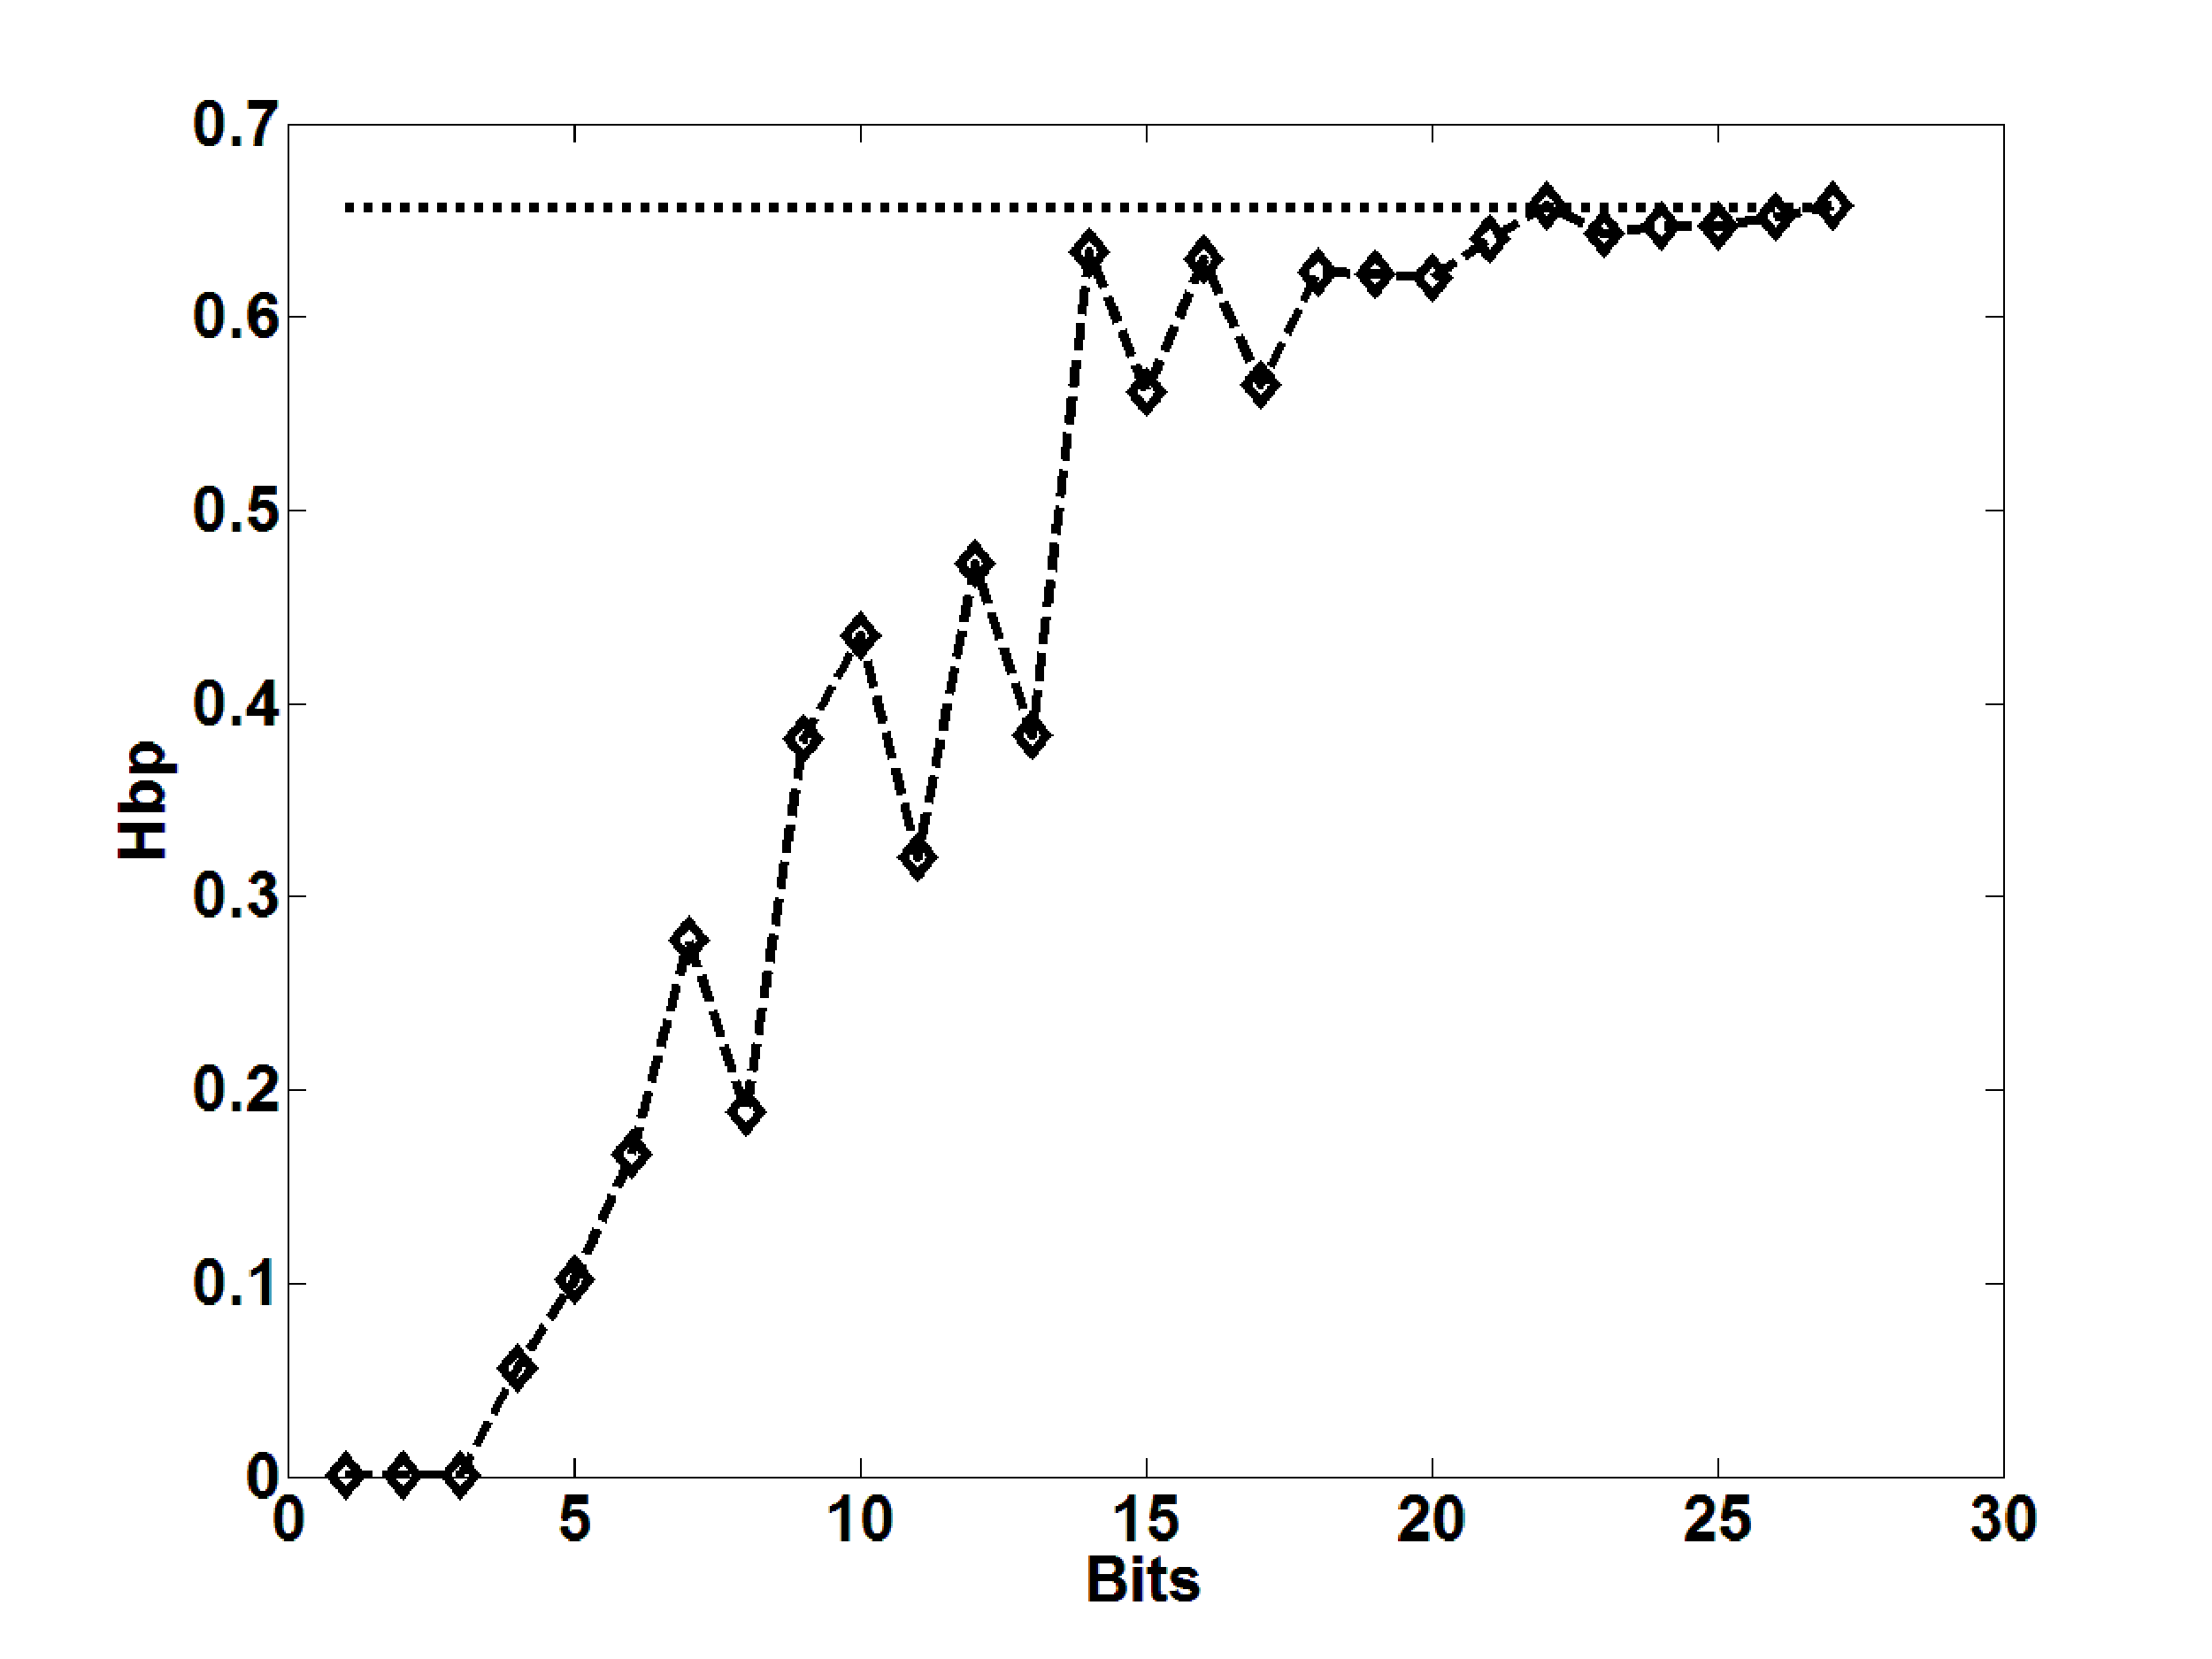
\includegraphics[width=0.3\textwidth]{Hbp_switchB2}
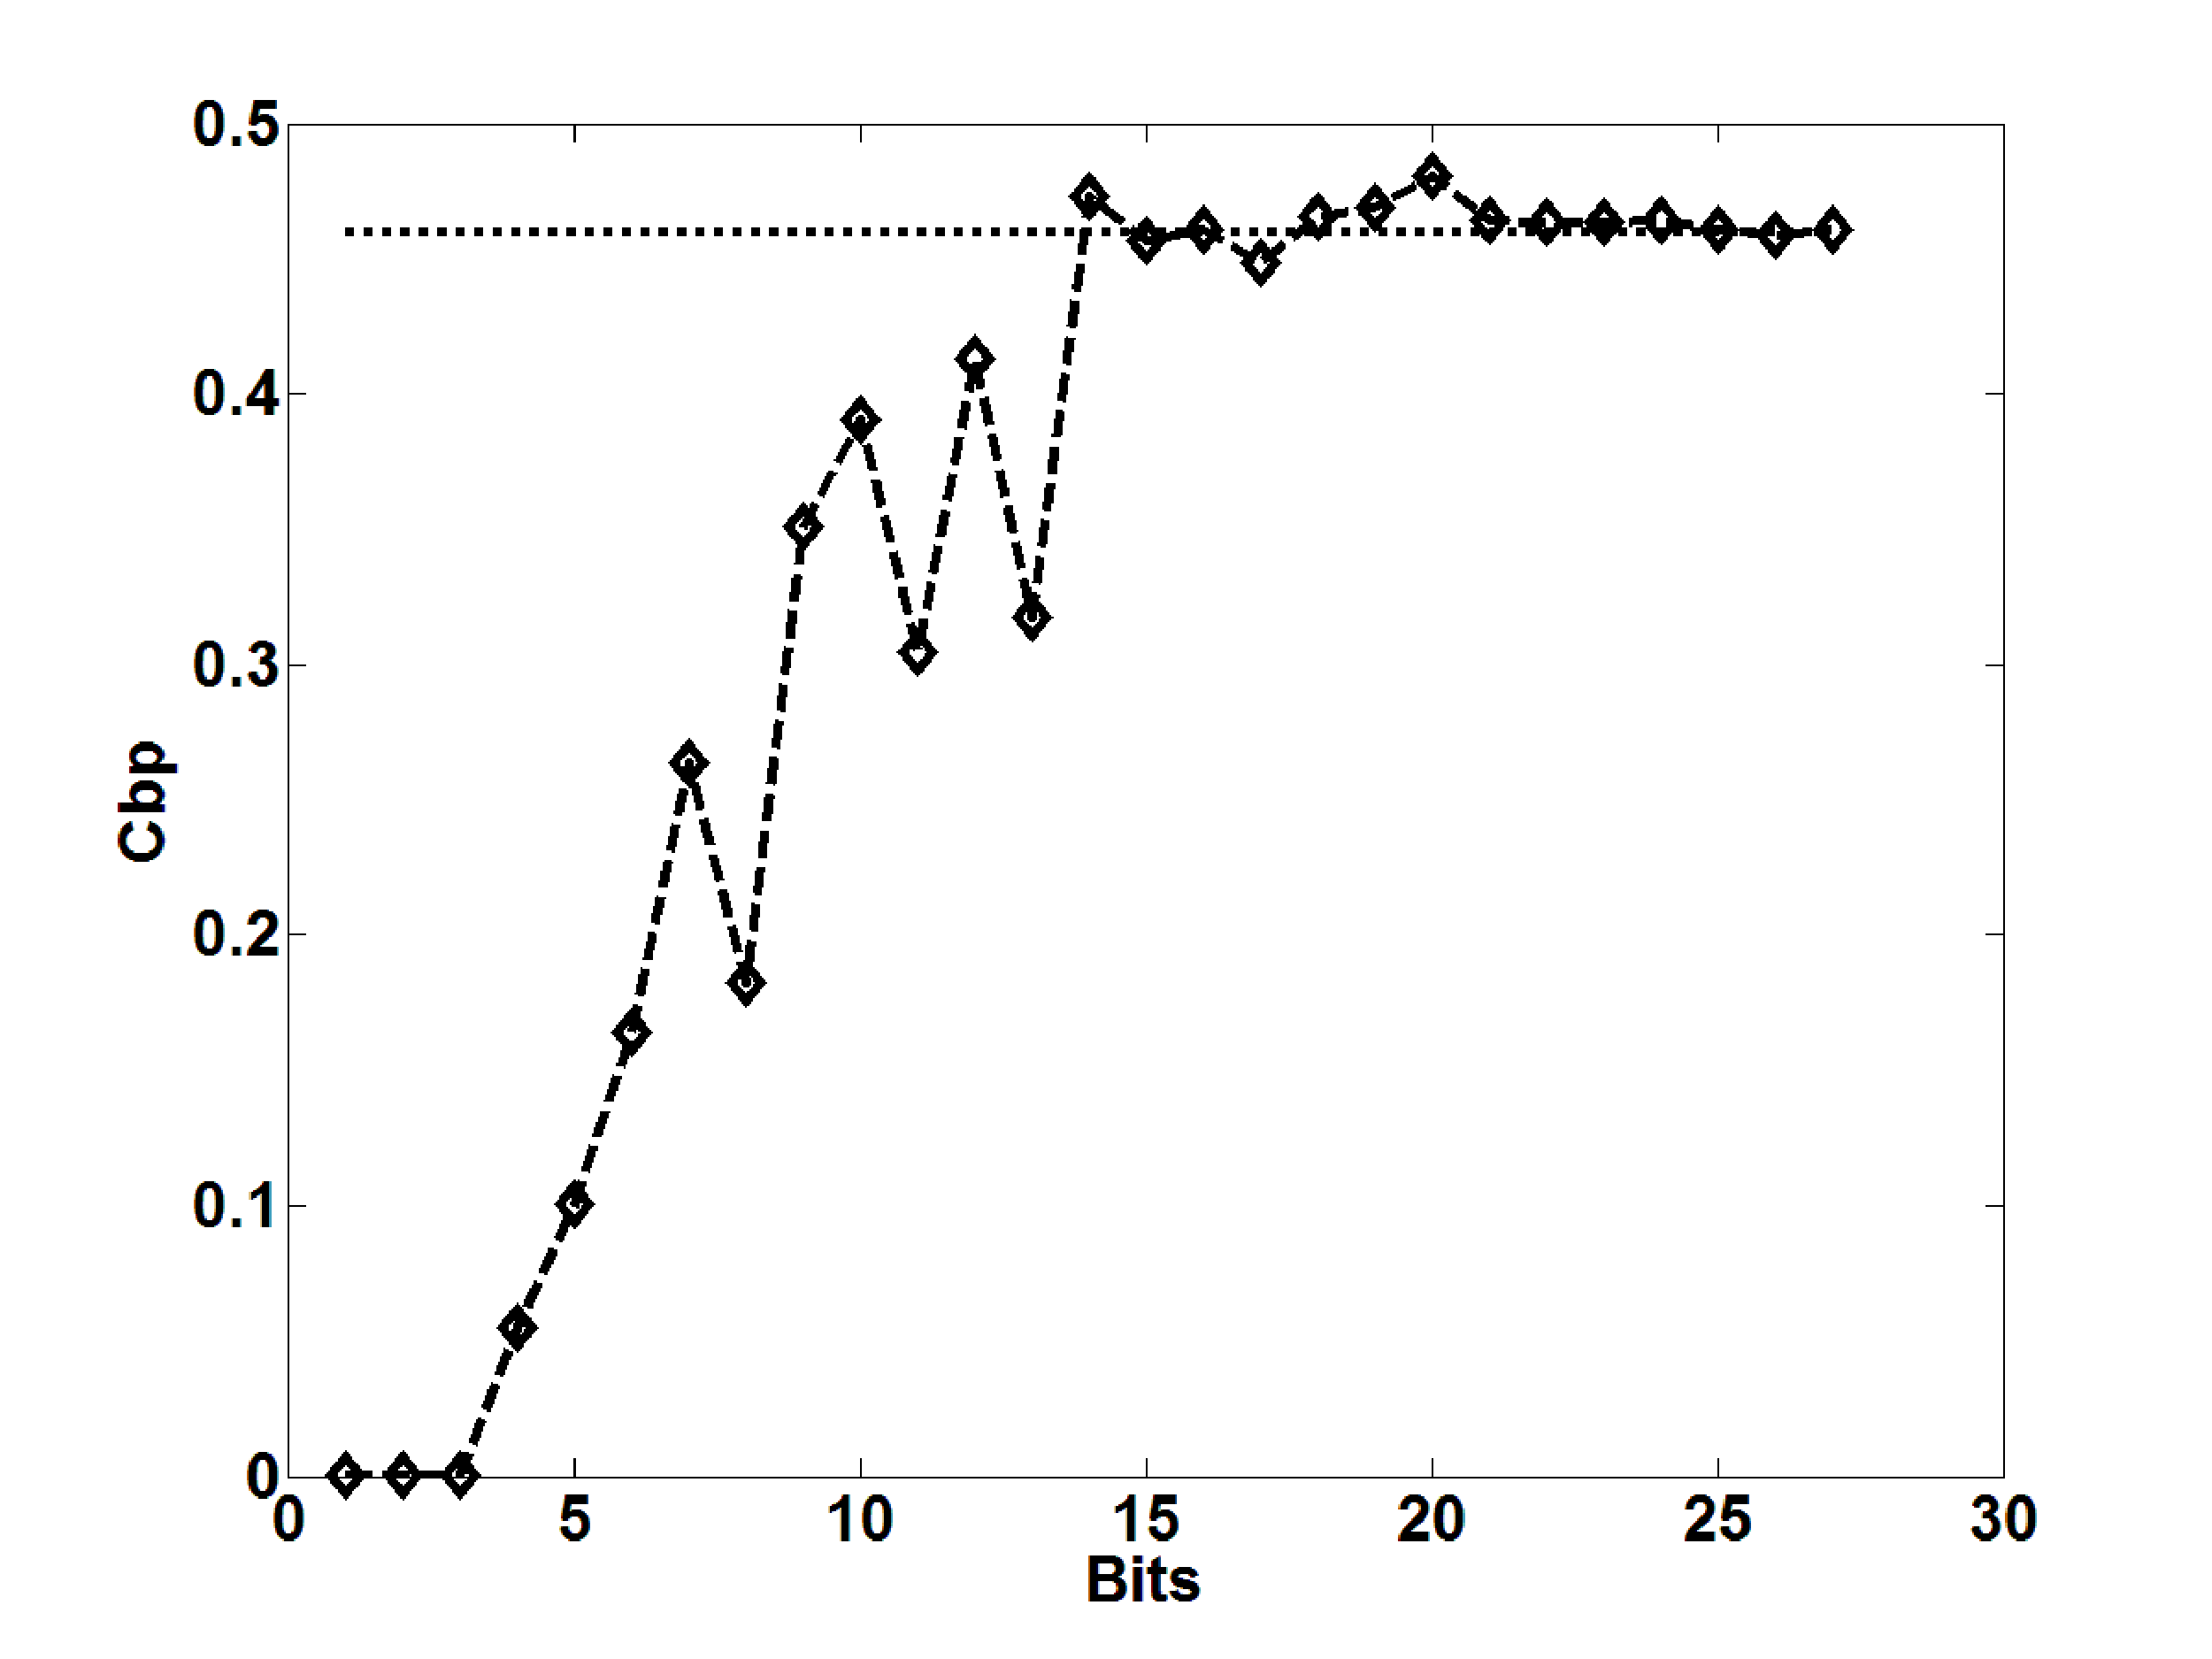
\includegraphics[width=0.3\textwidth]{Cbp_switchB2}
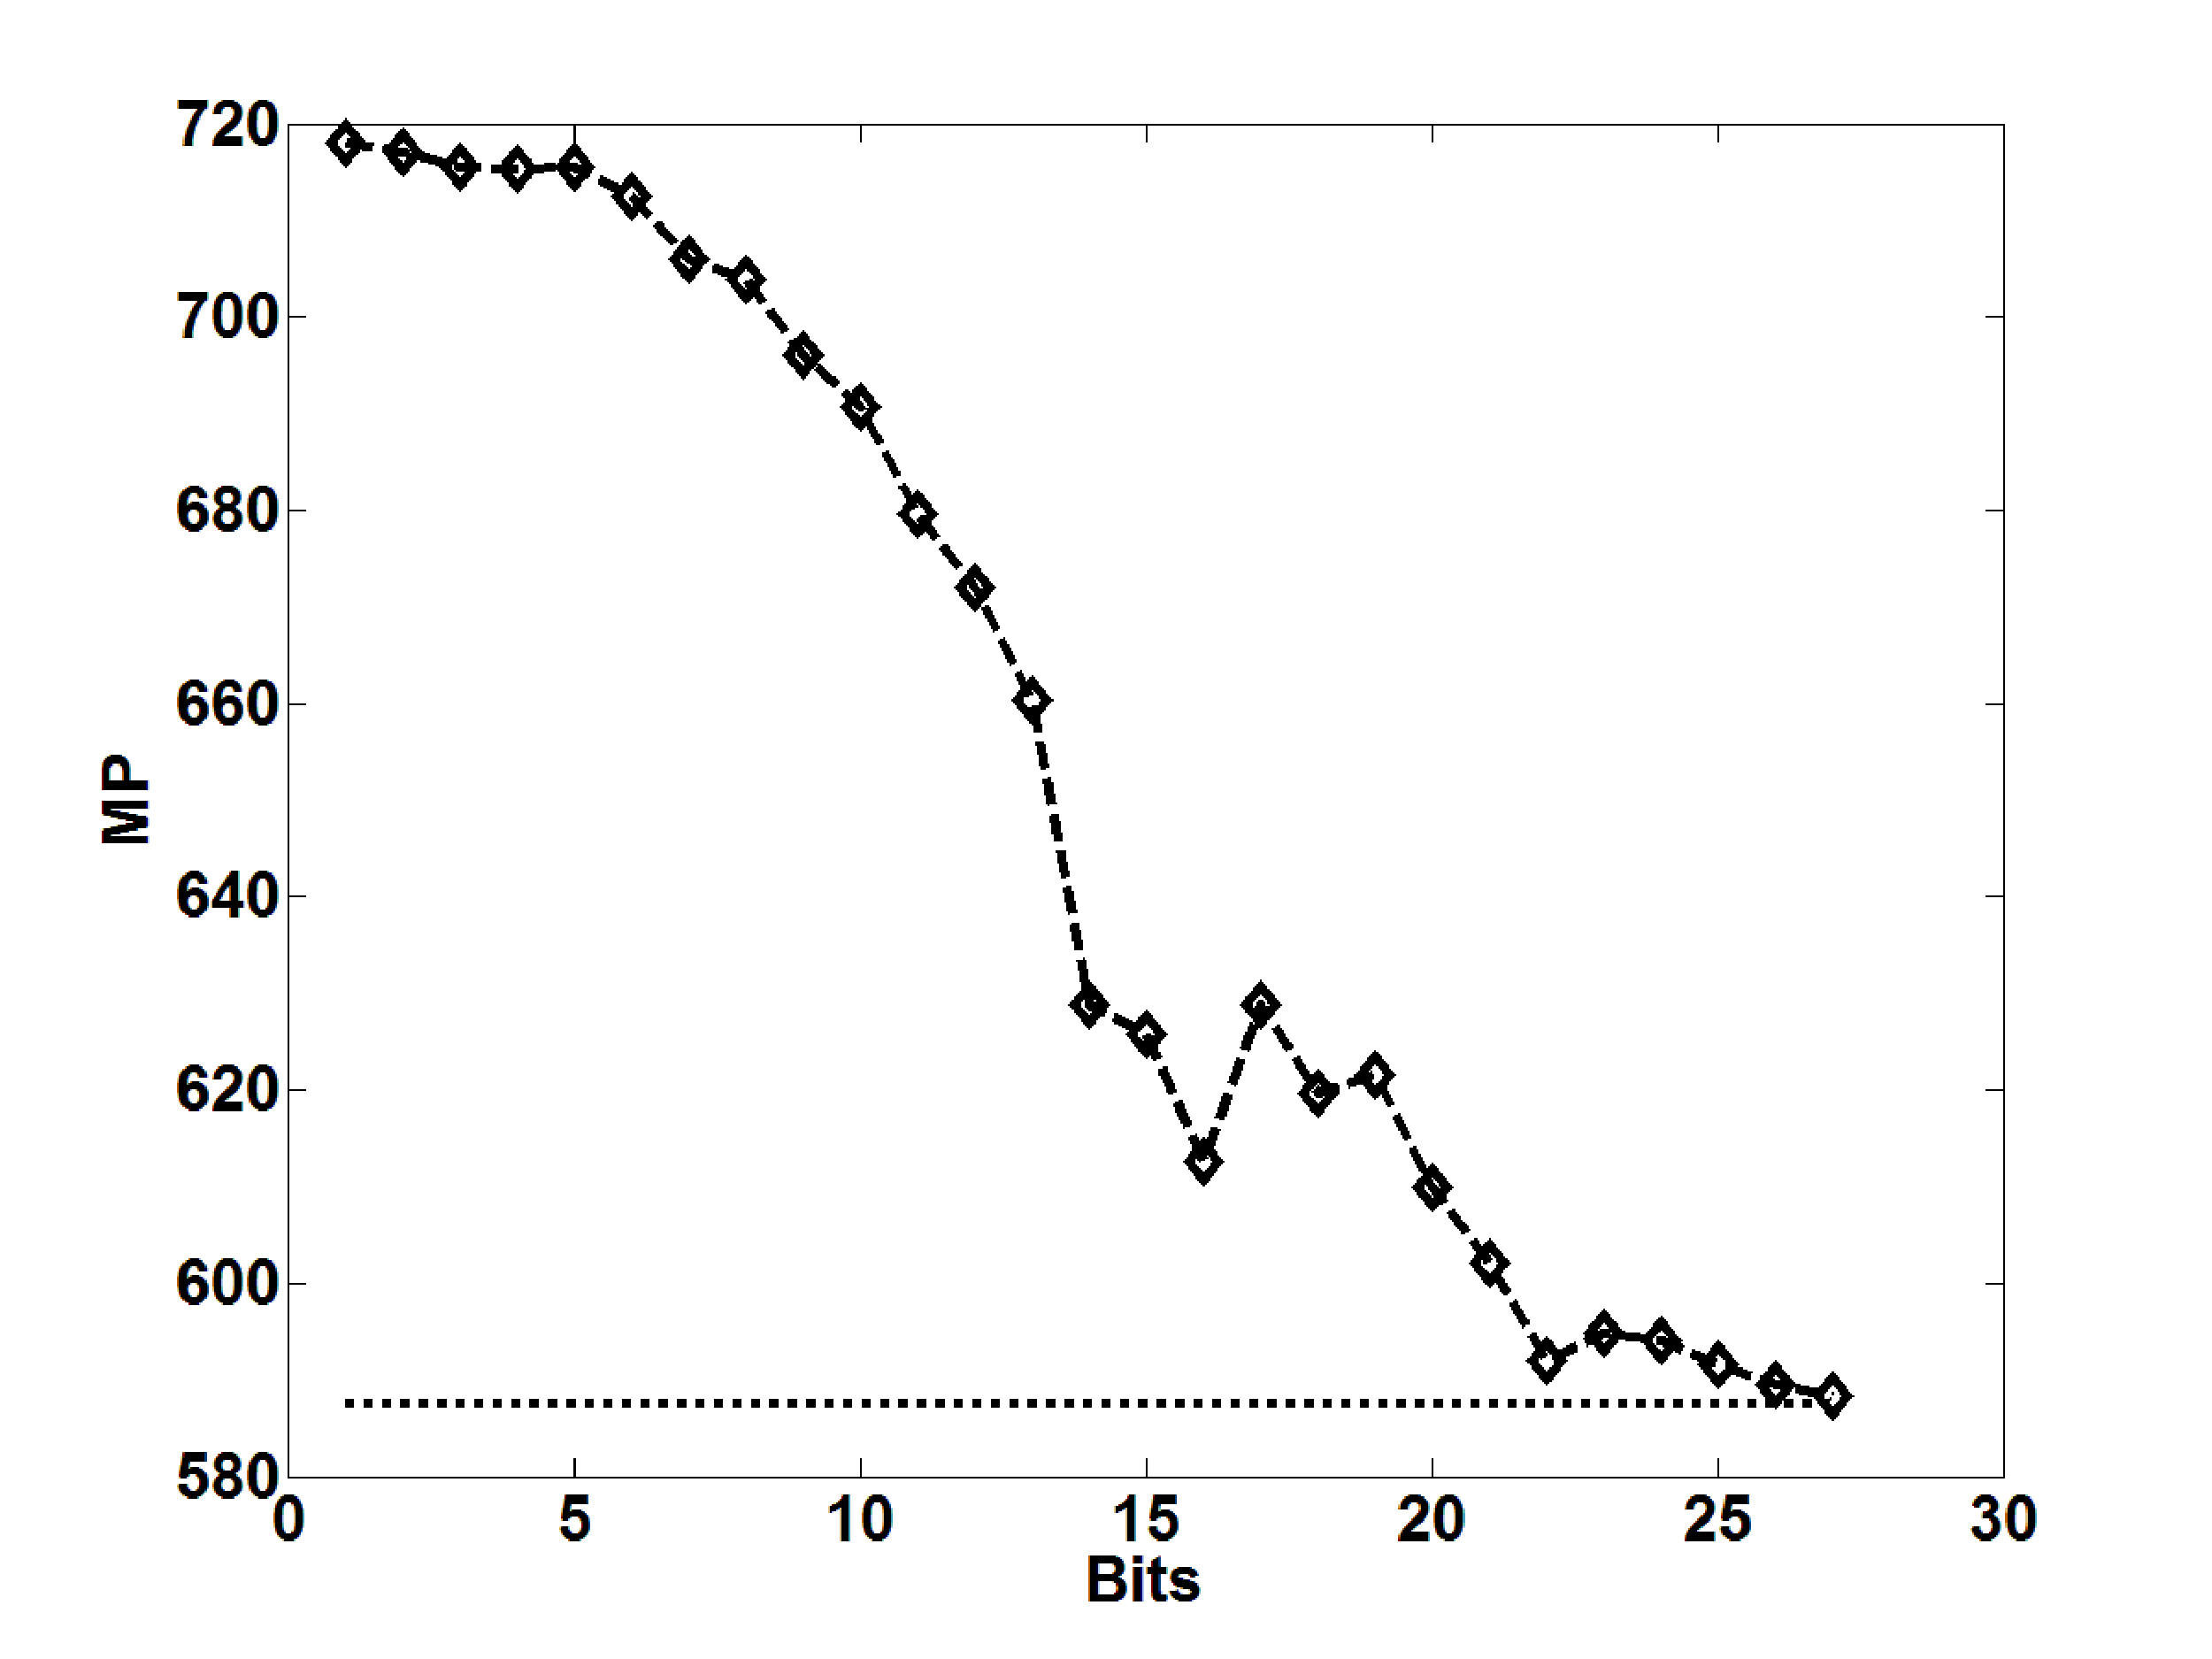
\includegraphics[width=0.3\textwidth]{Miss_switchB2}
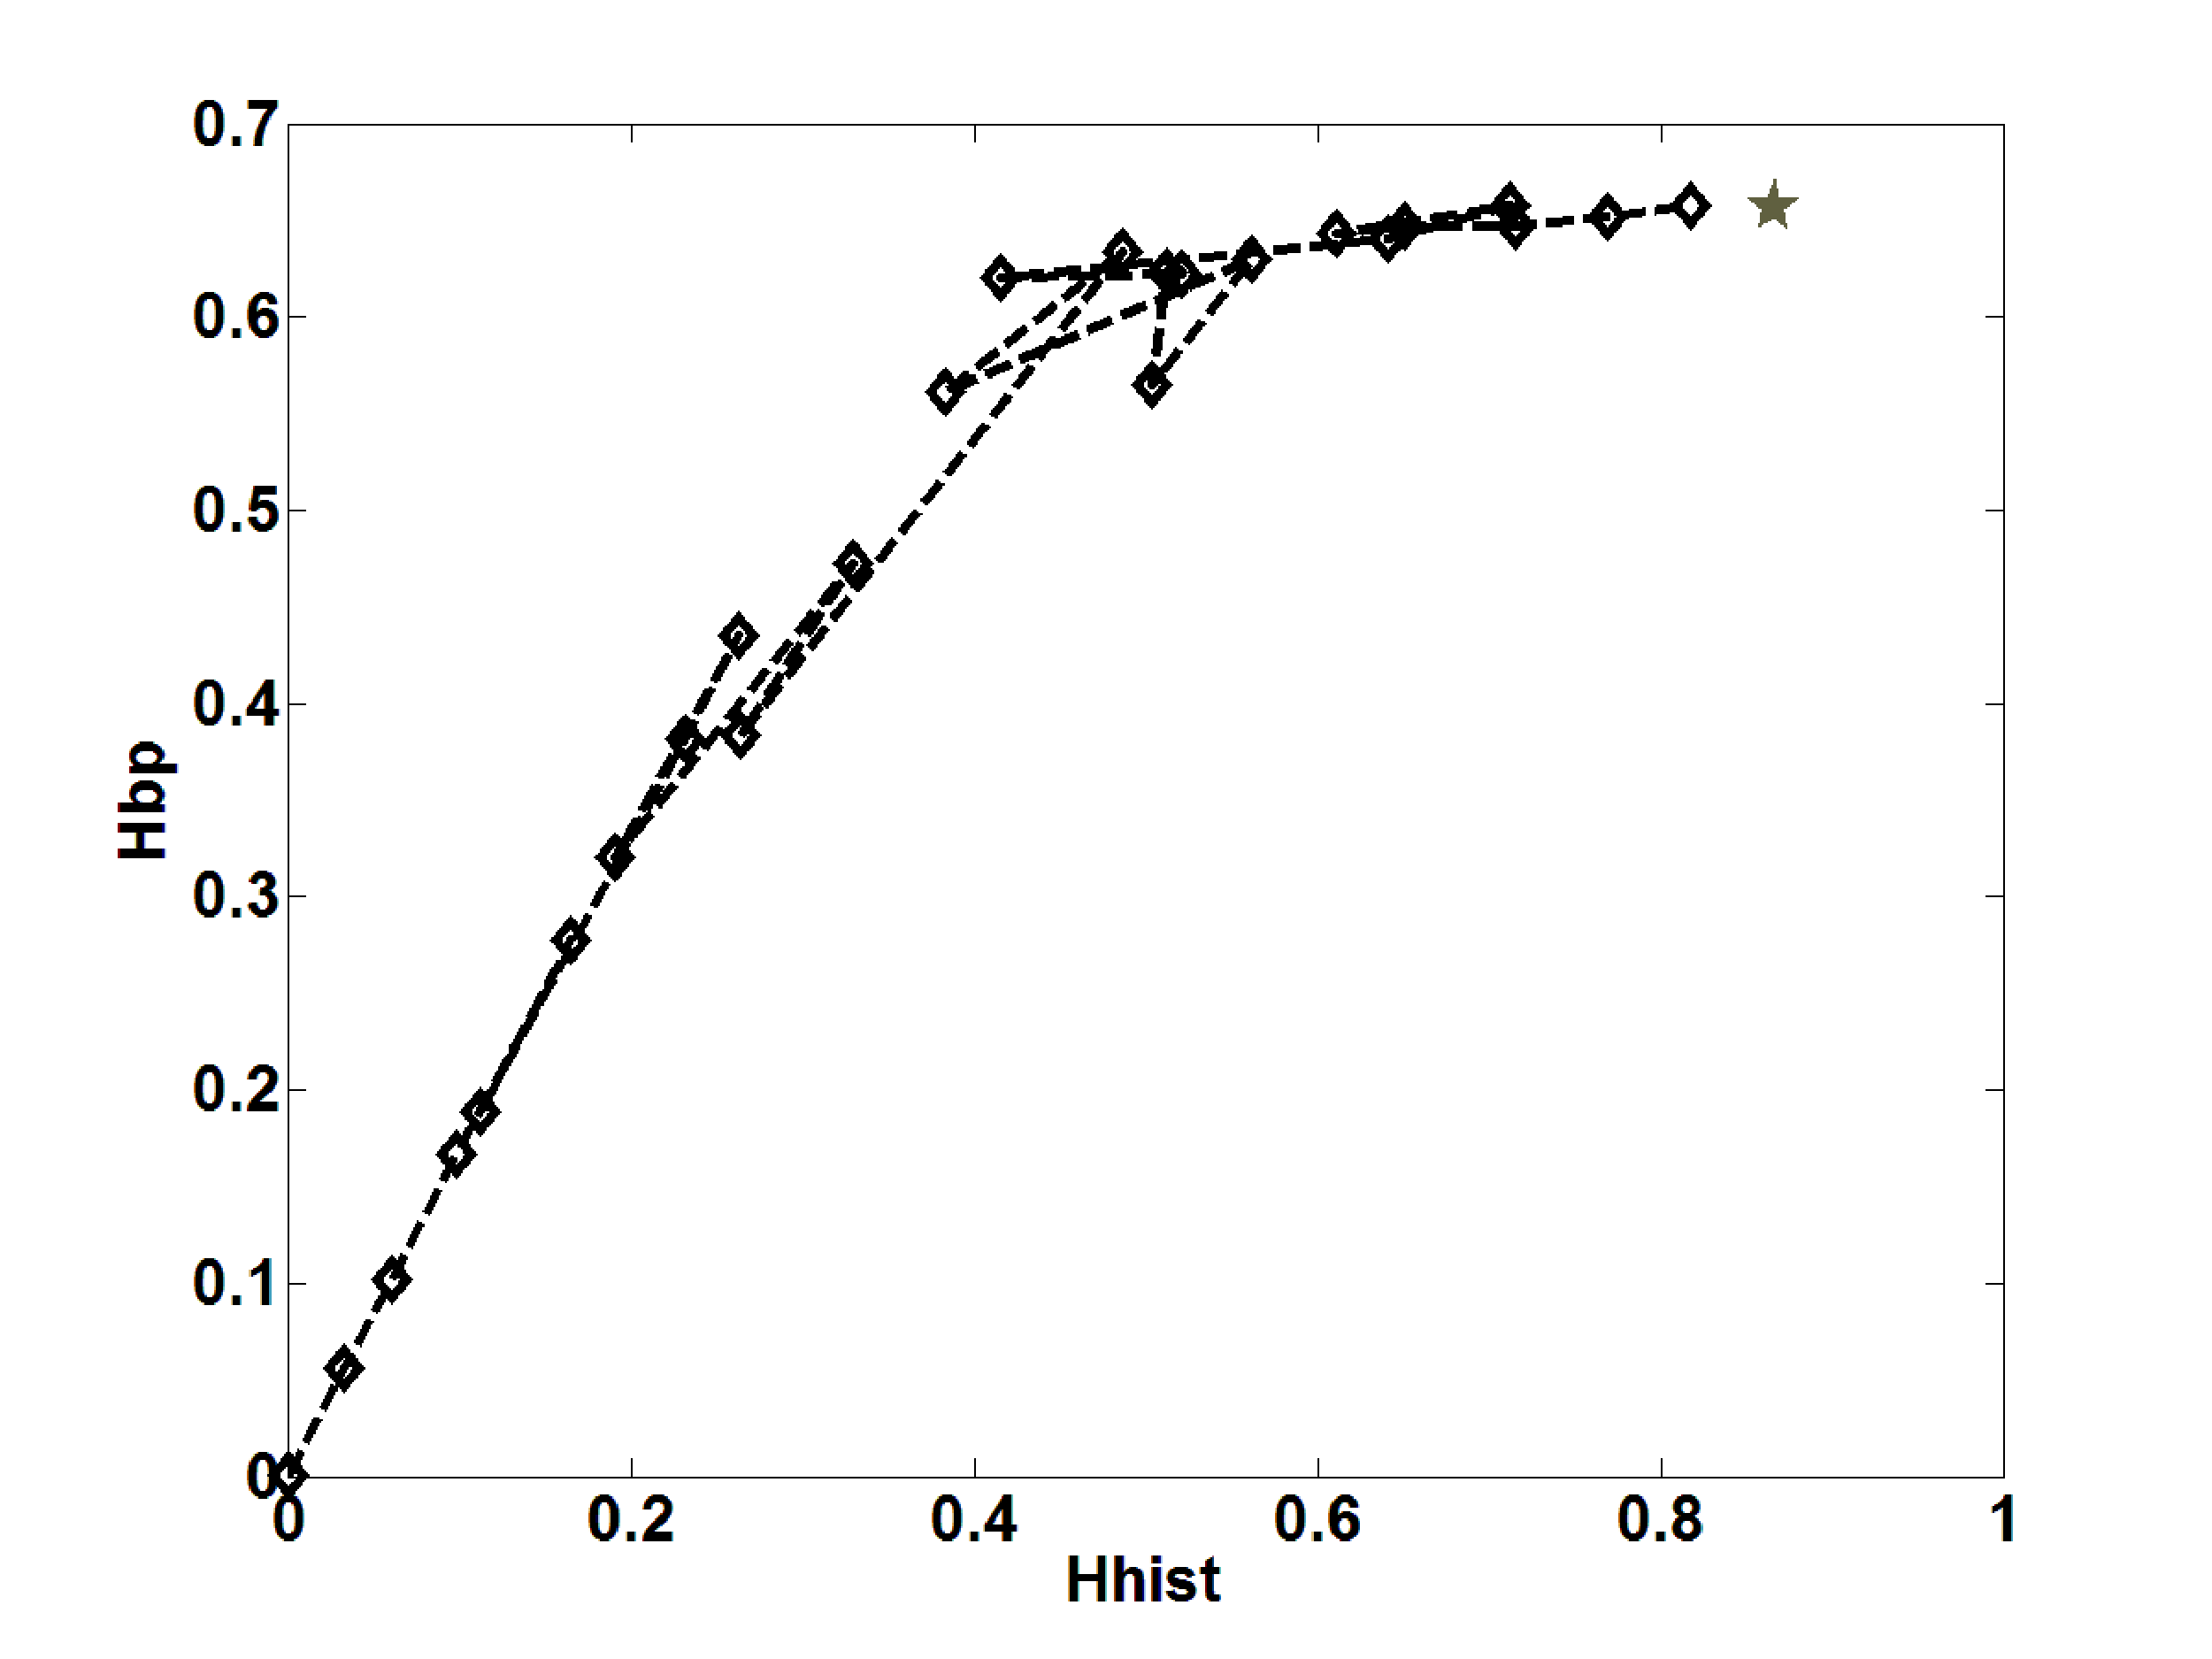
\includegraphics[width=0.3\textwidth]{HhistHbp_switchB2}
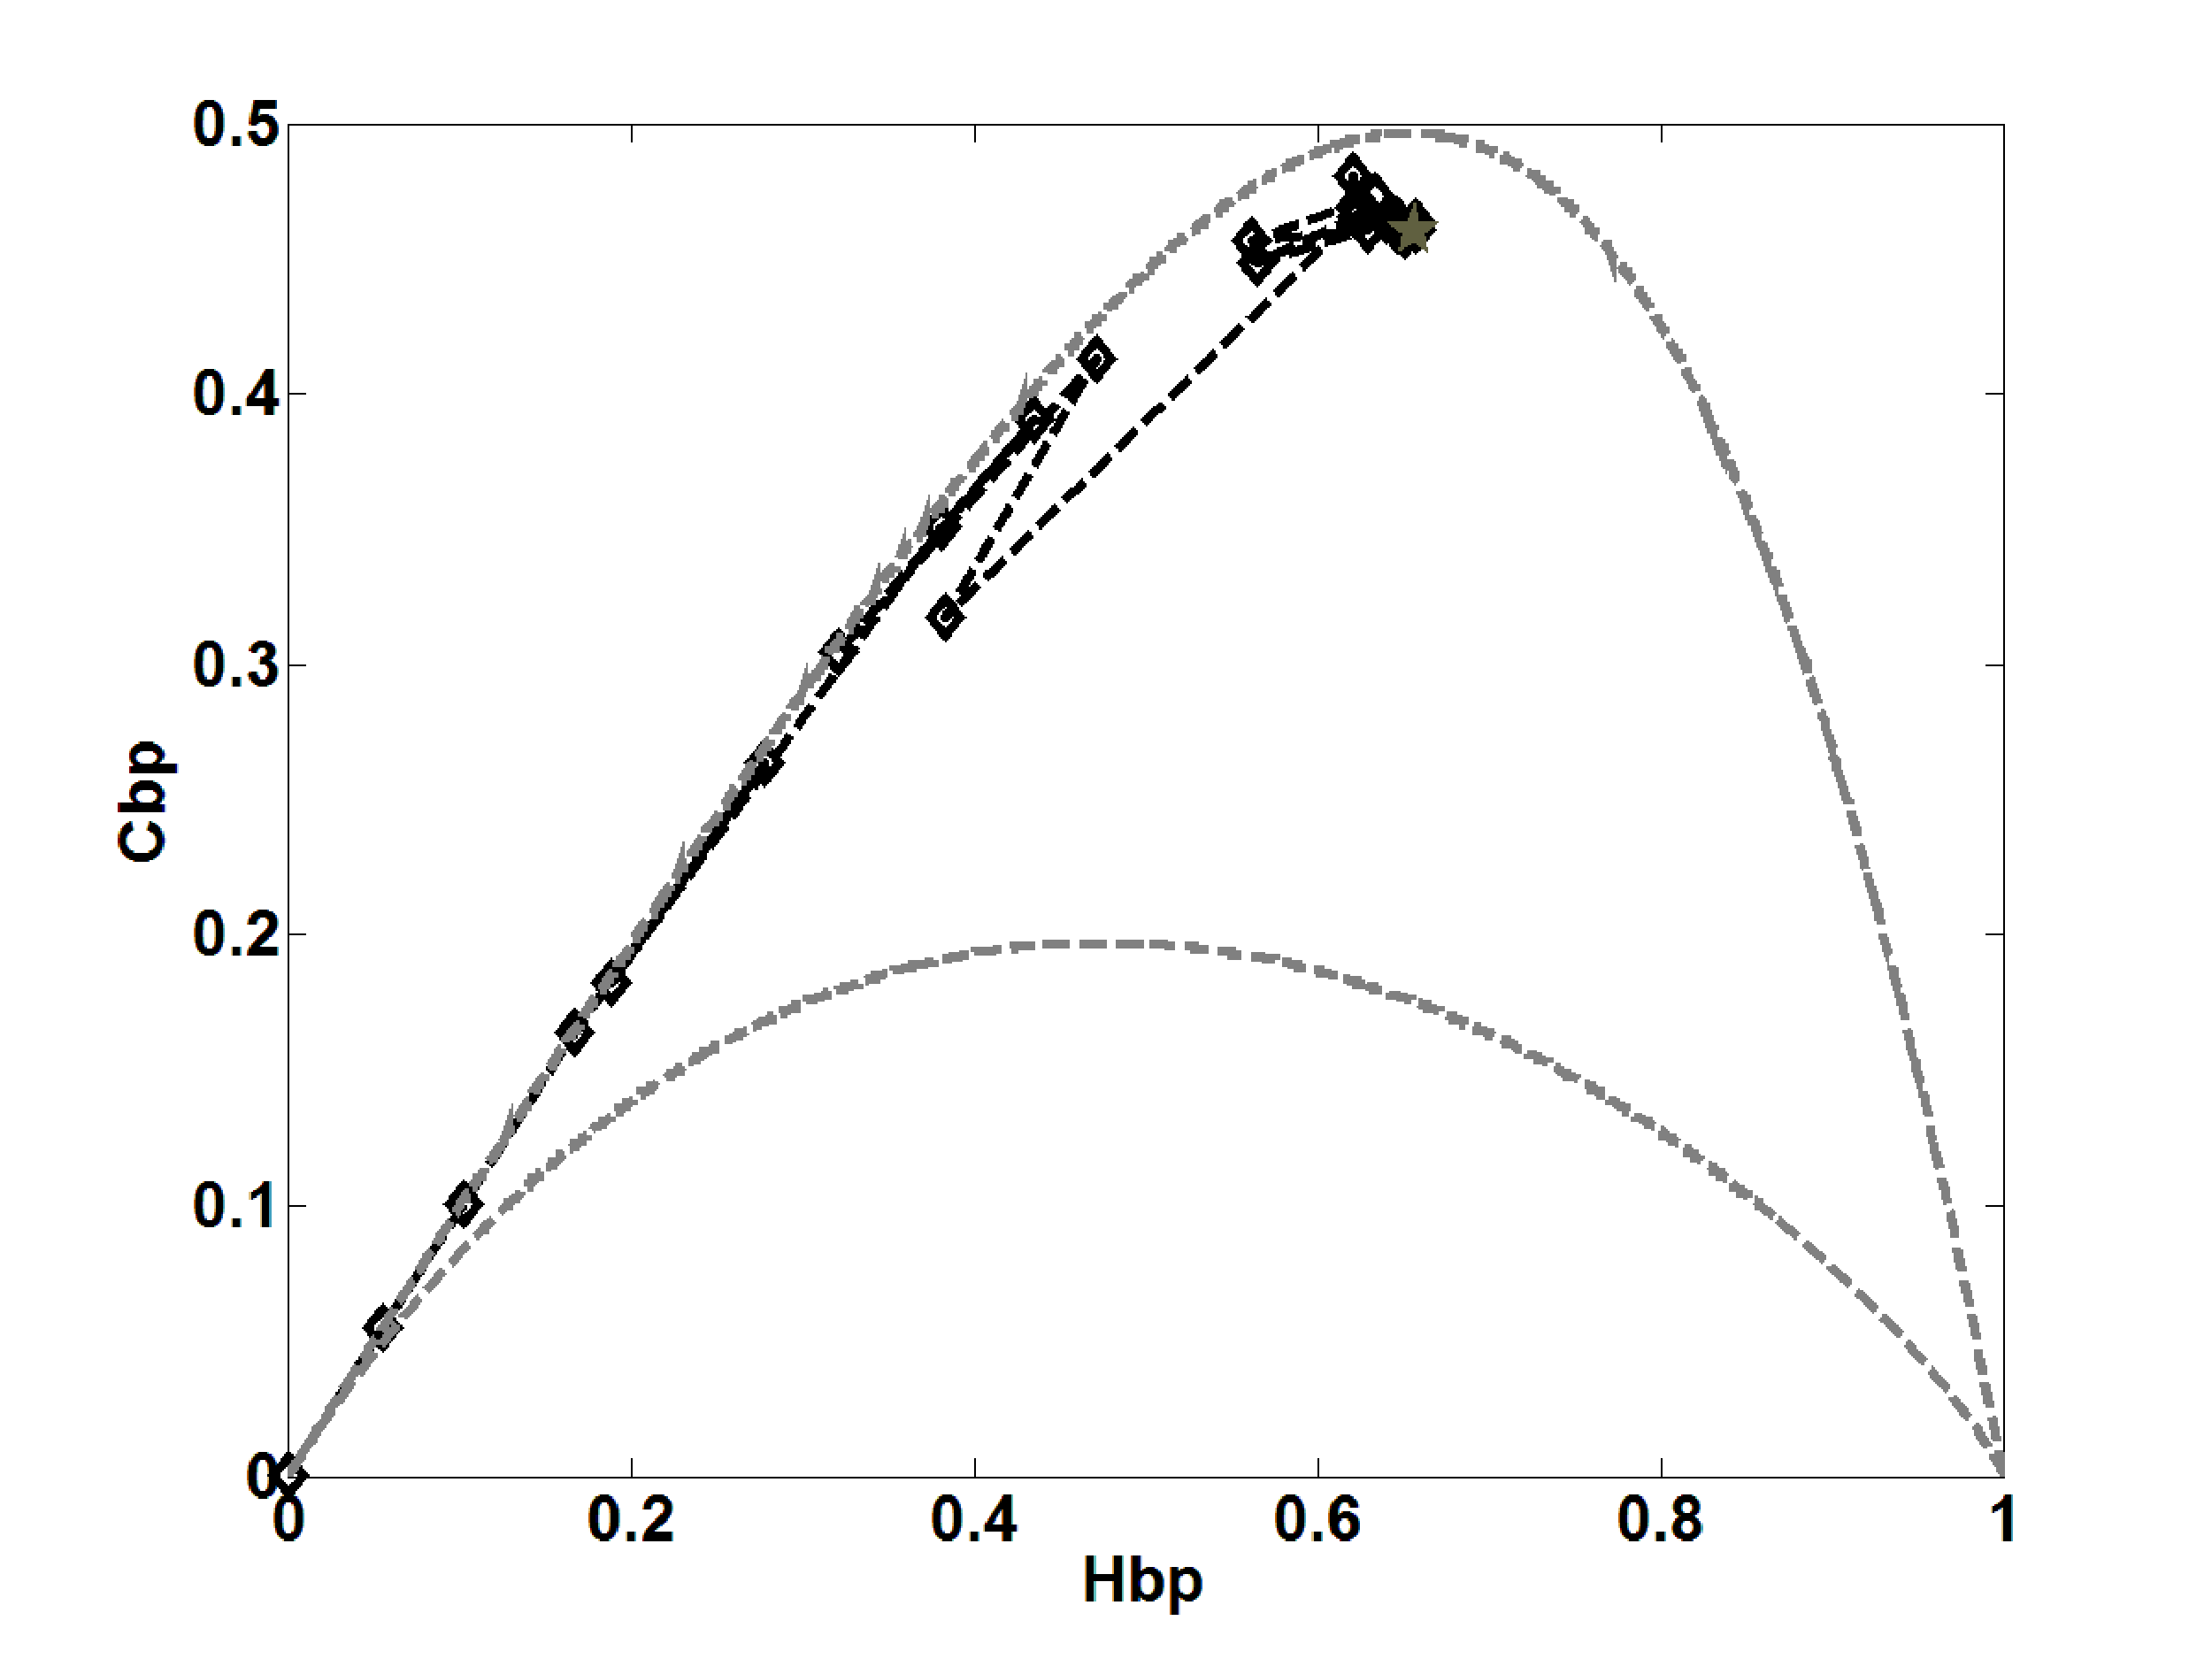
\includegraphics[width=0.3\textwidth]{HbpCbp_switchB2}
\caption{Statistical properties of the SWITCH map using binary representation: (a) $H_{hist}$ vs $P$ (b) $H_{BP}$ vs $P$ (c) $C_{BP}$ vs $P$ (d) Number of missing ordering patterns $MP$ vs $P$. In Figures (a) to (d) dashed line correspond to floating point numbers. (e) representation in the $H_{hist},H_{BP}$ plane in the the binary numerical system.  The star represents the state for floating points numbers. (f) representation in the $H_{BP},C_{BP}$ plane.  The star represents the state for floating points numbers. (The star represents the state for floating points numbers). } \label{fig:seqbin}
\end{figure}

%%%%%%%%%%%%%%%%%%%%%%%%%%
%%%%%%%%%%%%%%%%%%%%%%%%%%% Fig.7
\begin{figure}
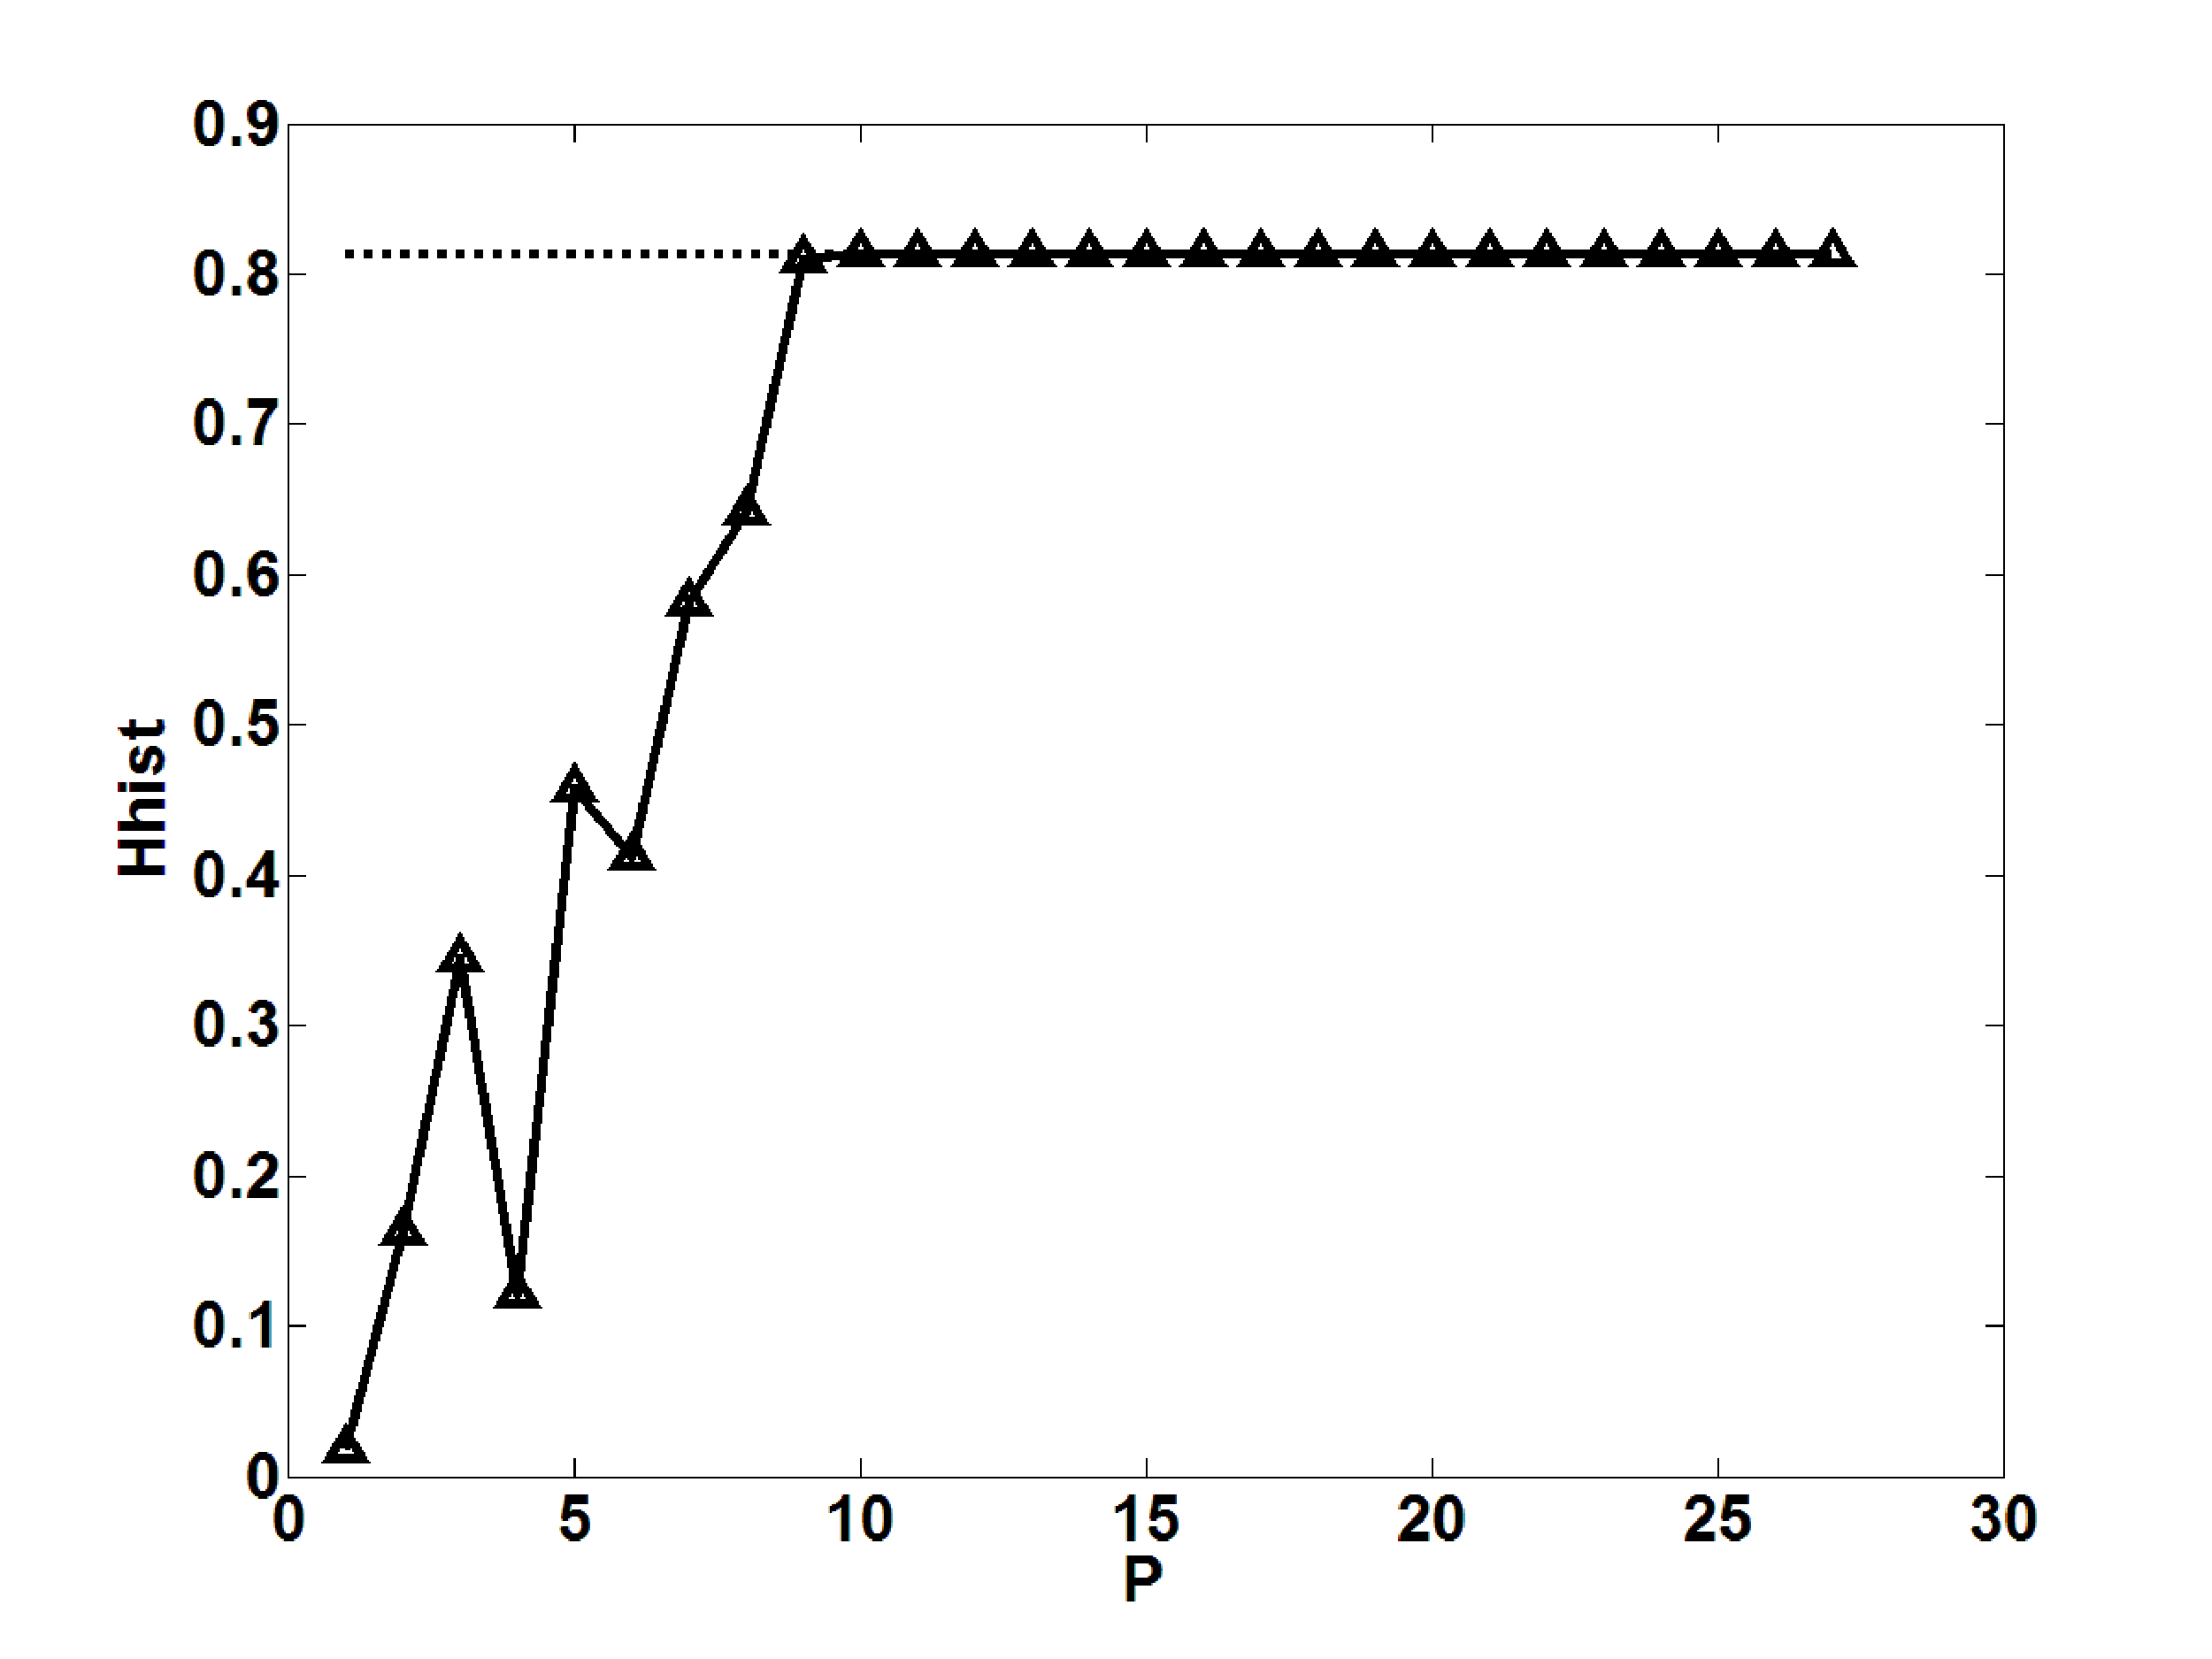
\includegraphics[width=0.3\textwidth]{Hhist_parB10}
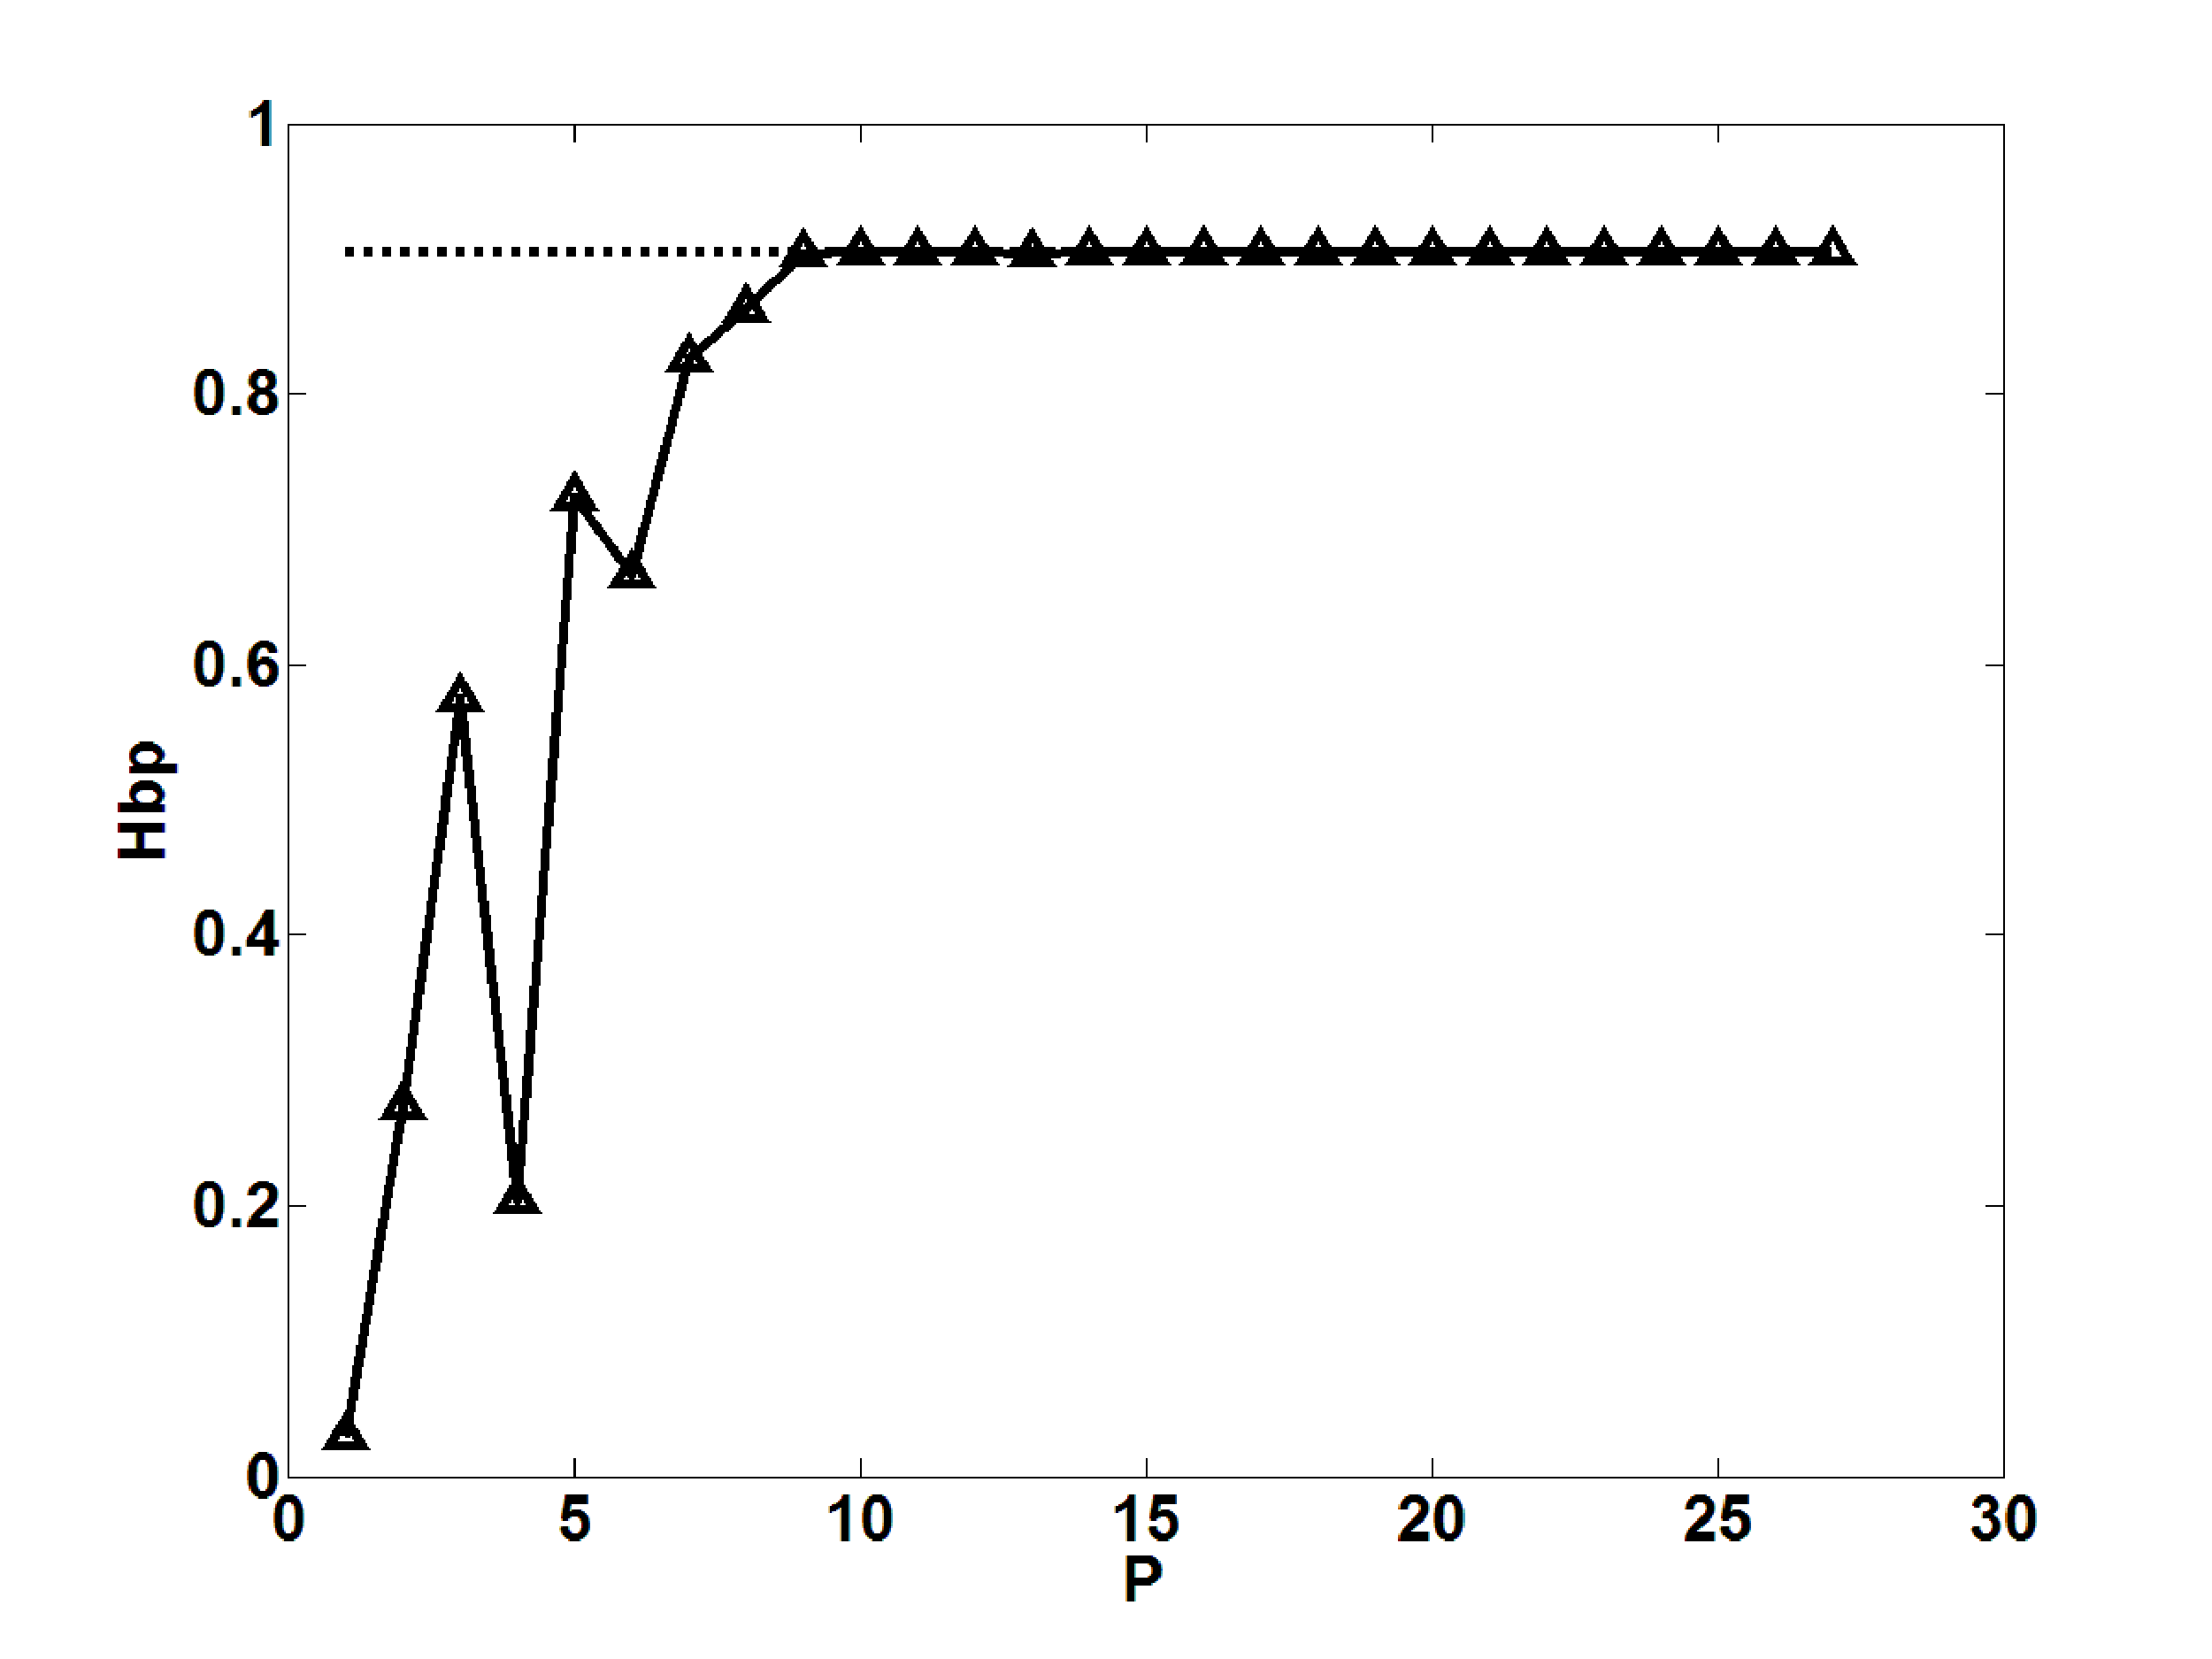
\includegraphics[width=0.3\textwidth]{Hbp_parB10}
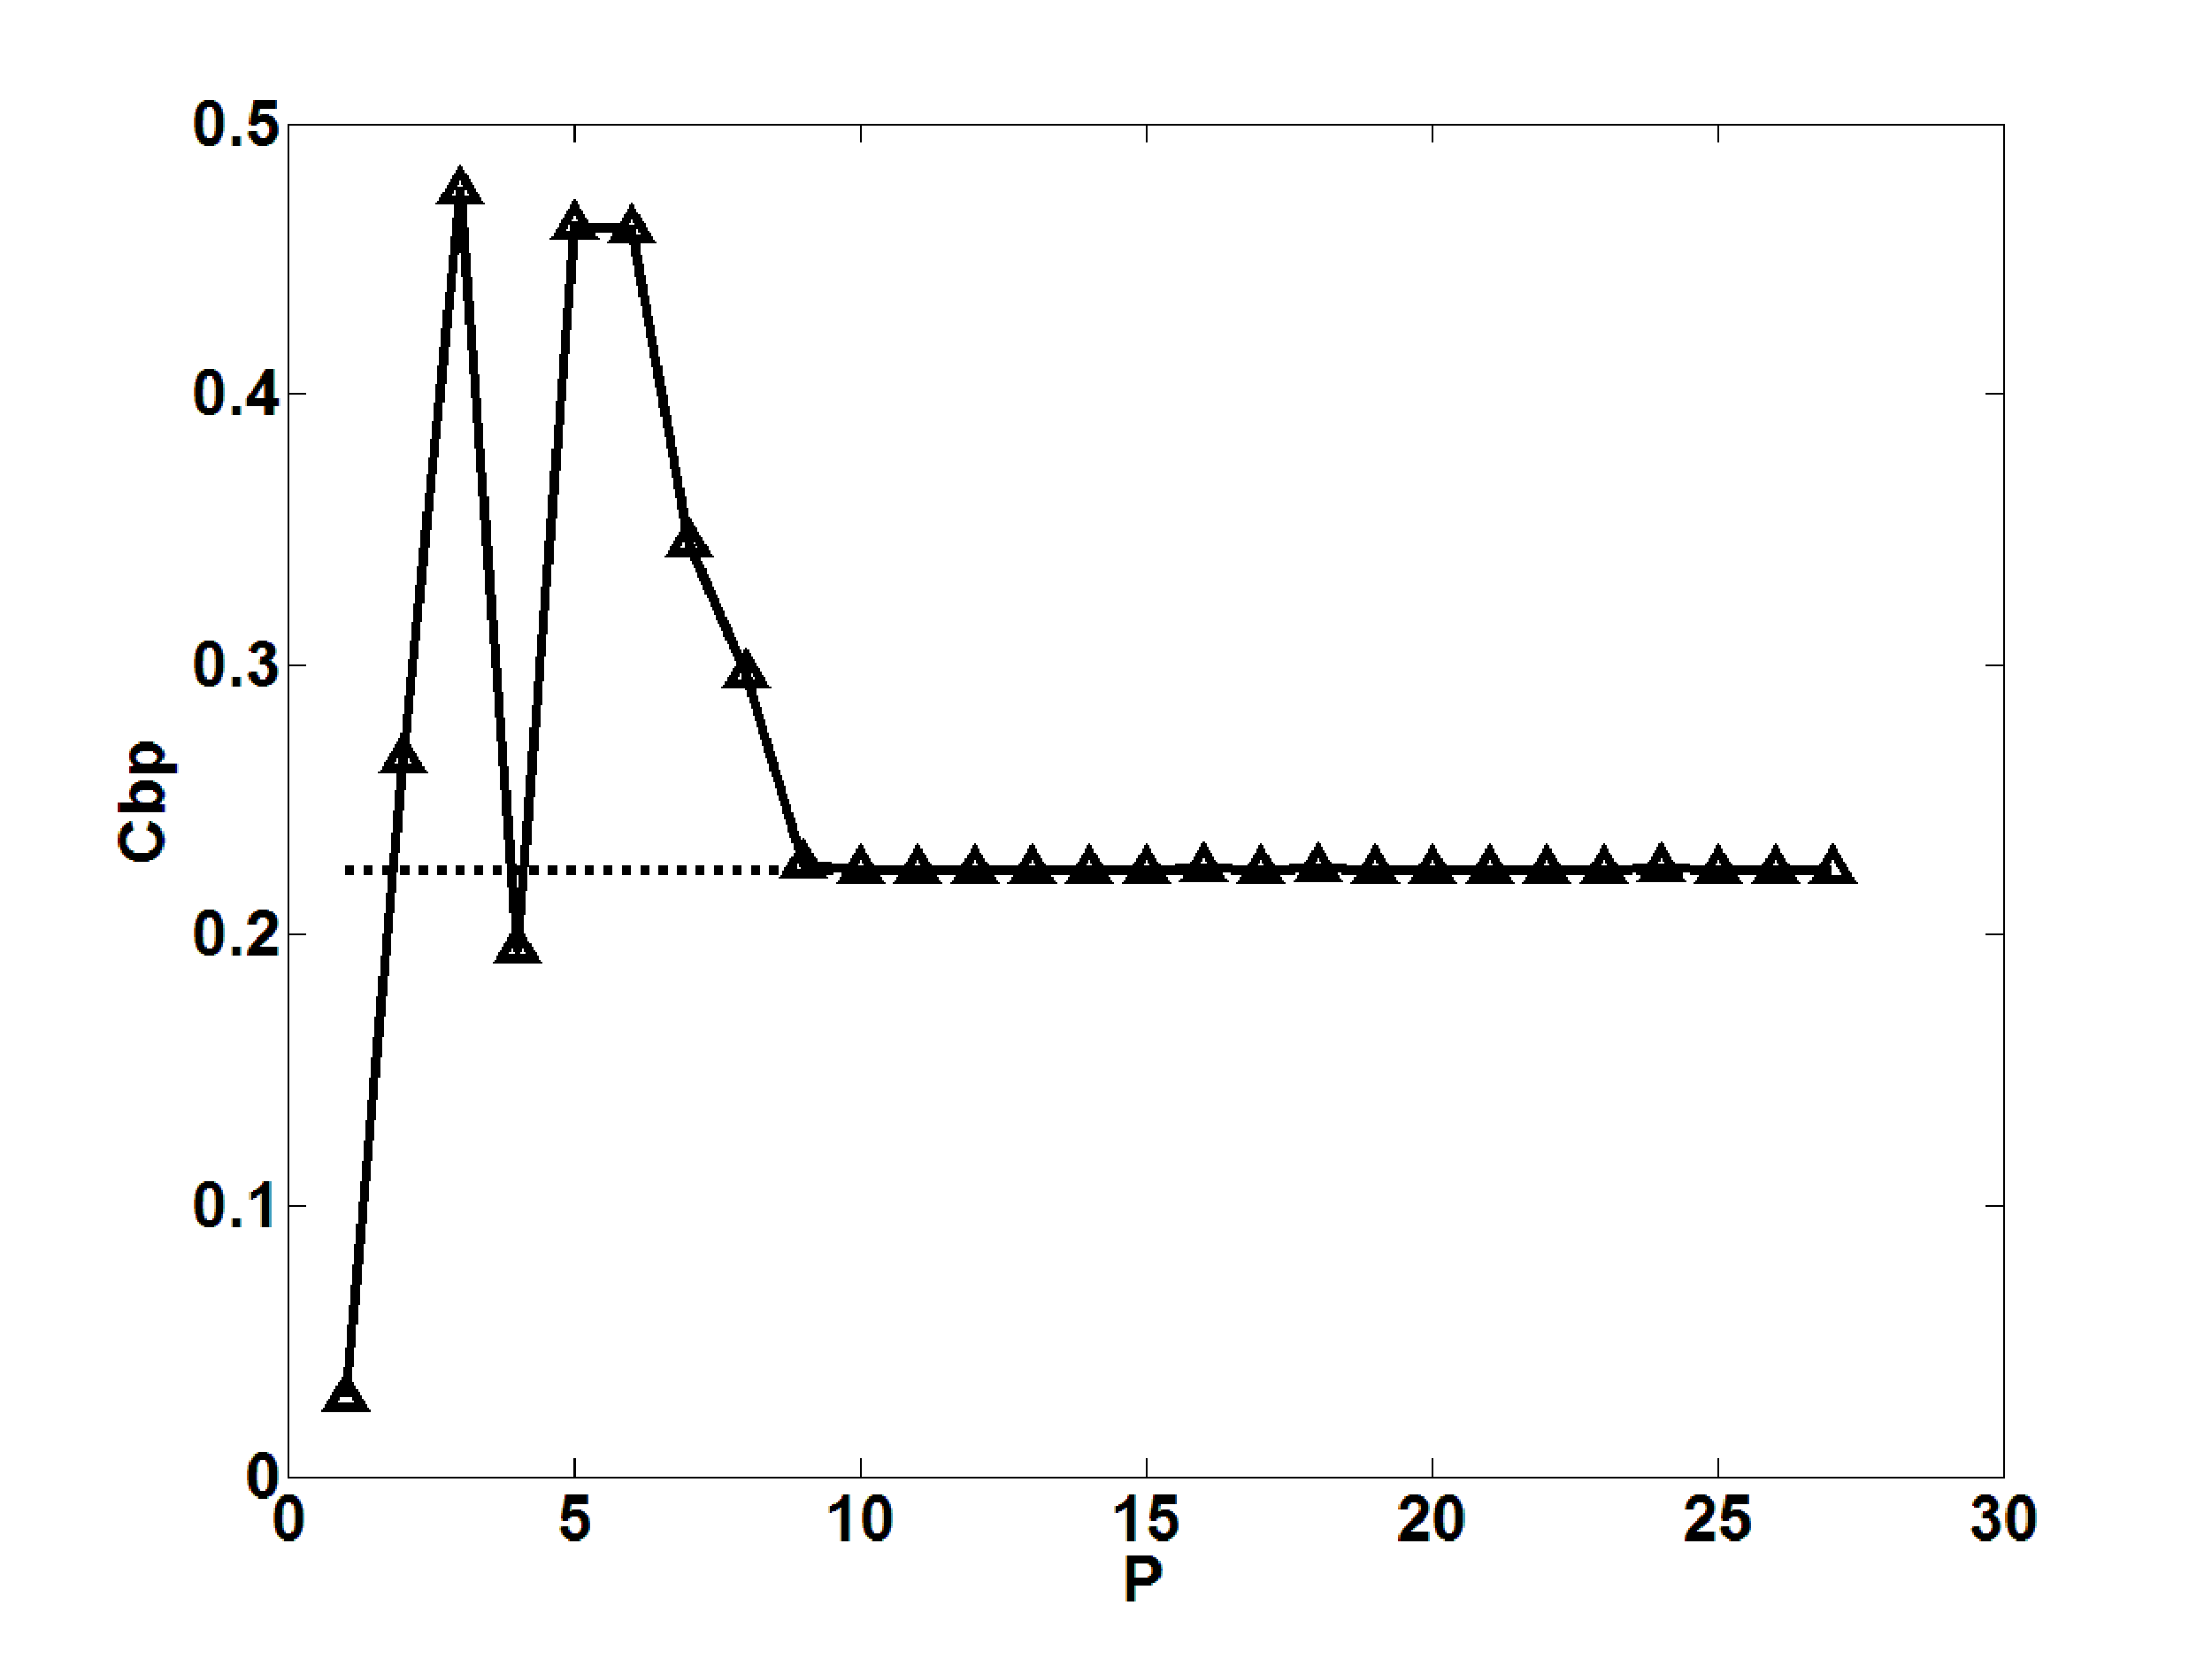
\includegraphics[width=0.3\textwidth]{Cbp_parB10}
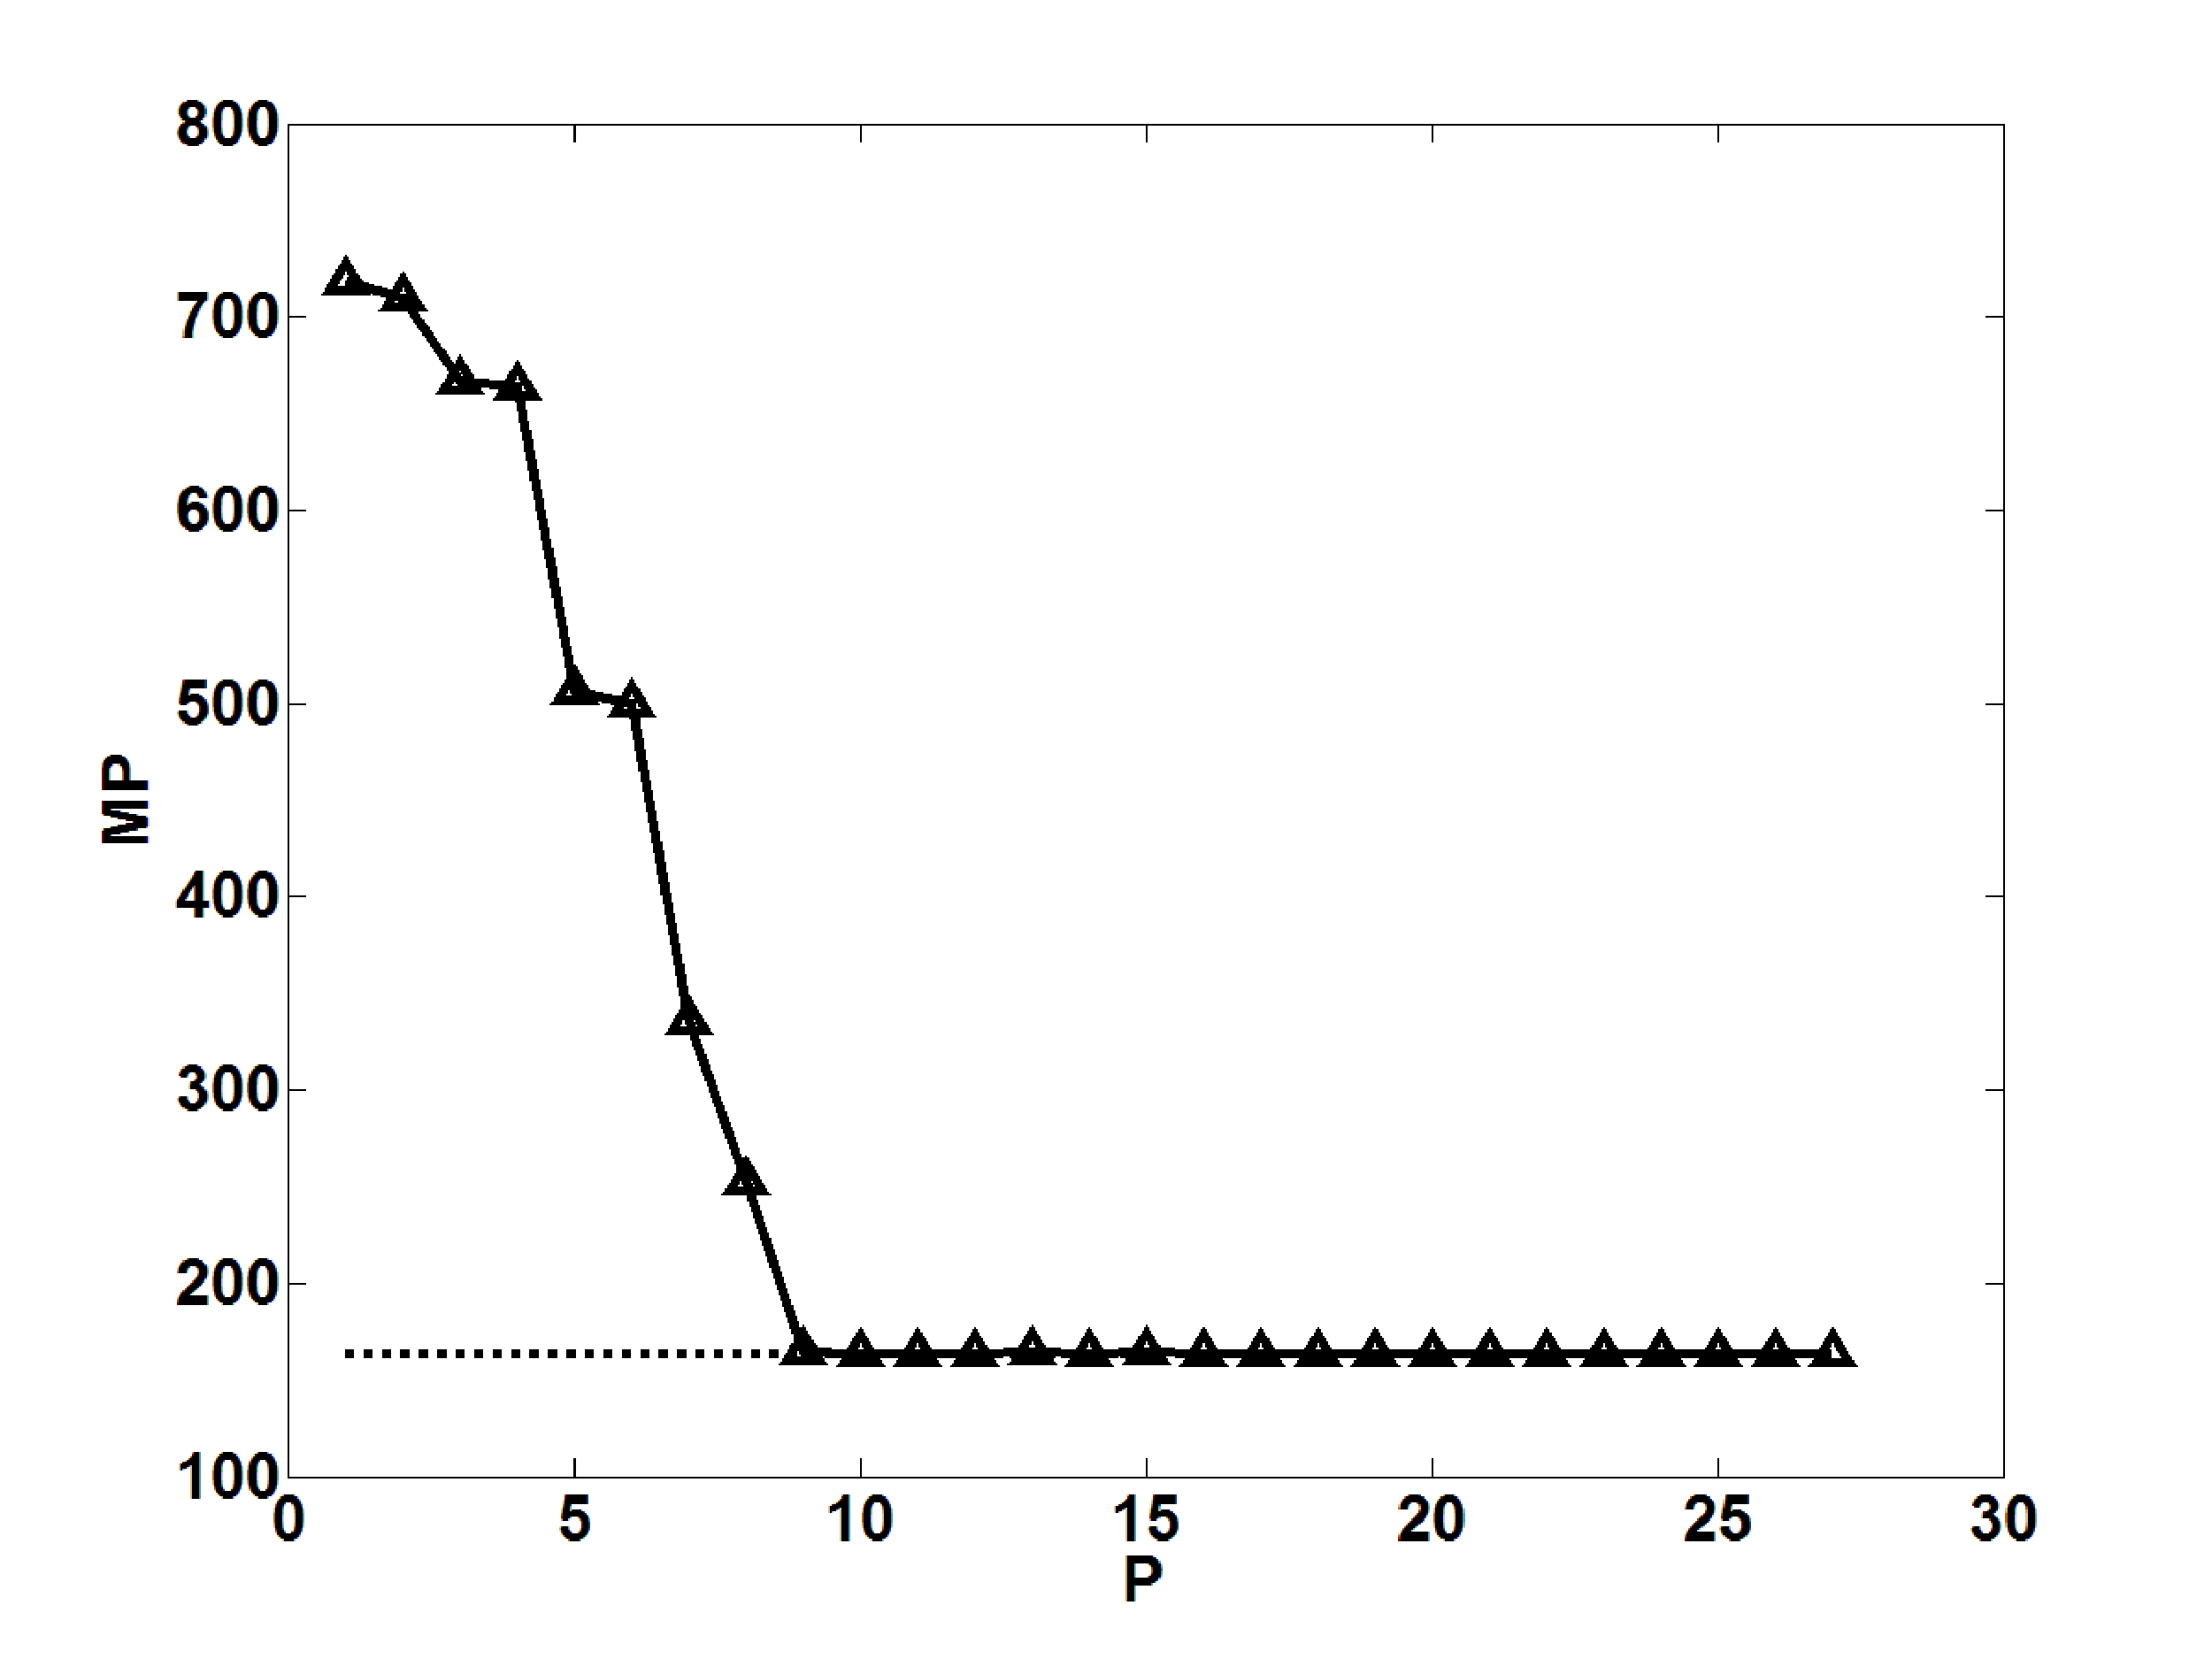
\includegraphics[width=0.3\textwidth]{Miss_parB10}
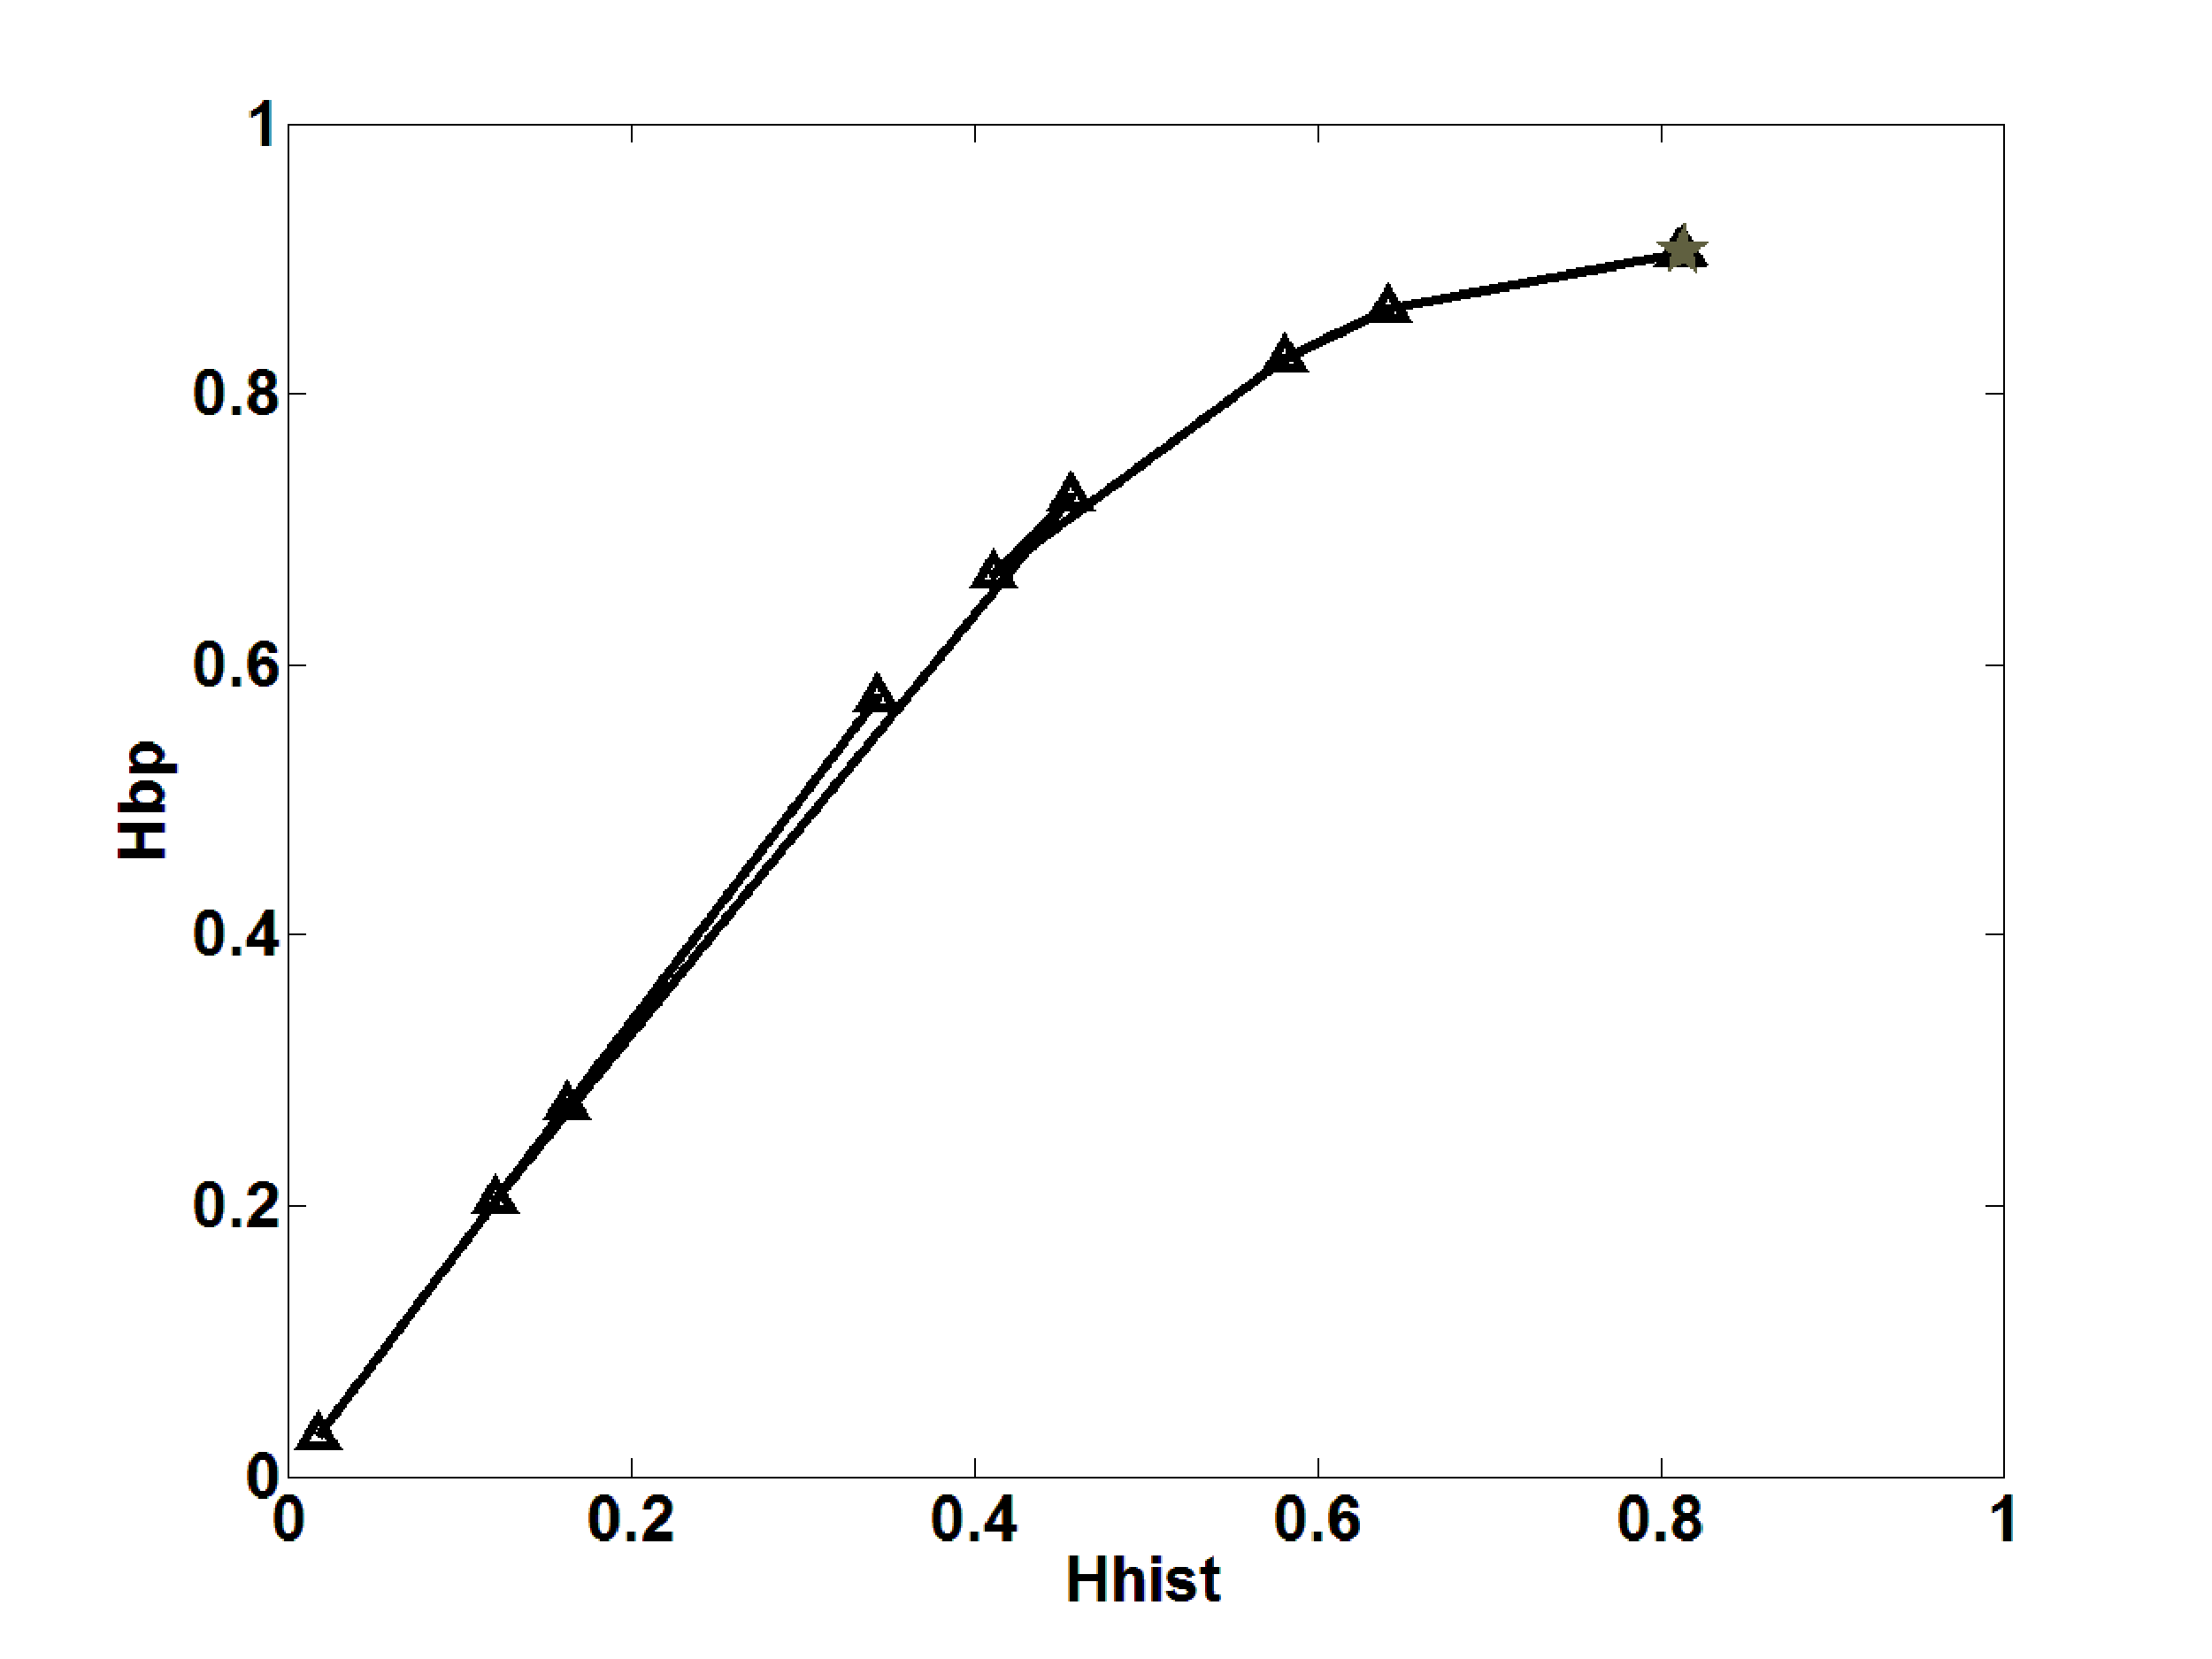
\includegraphics[width=0.3\textwidth]{HhistHbp_parB10}
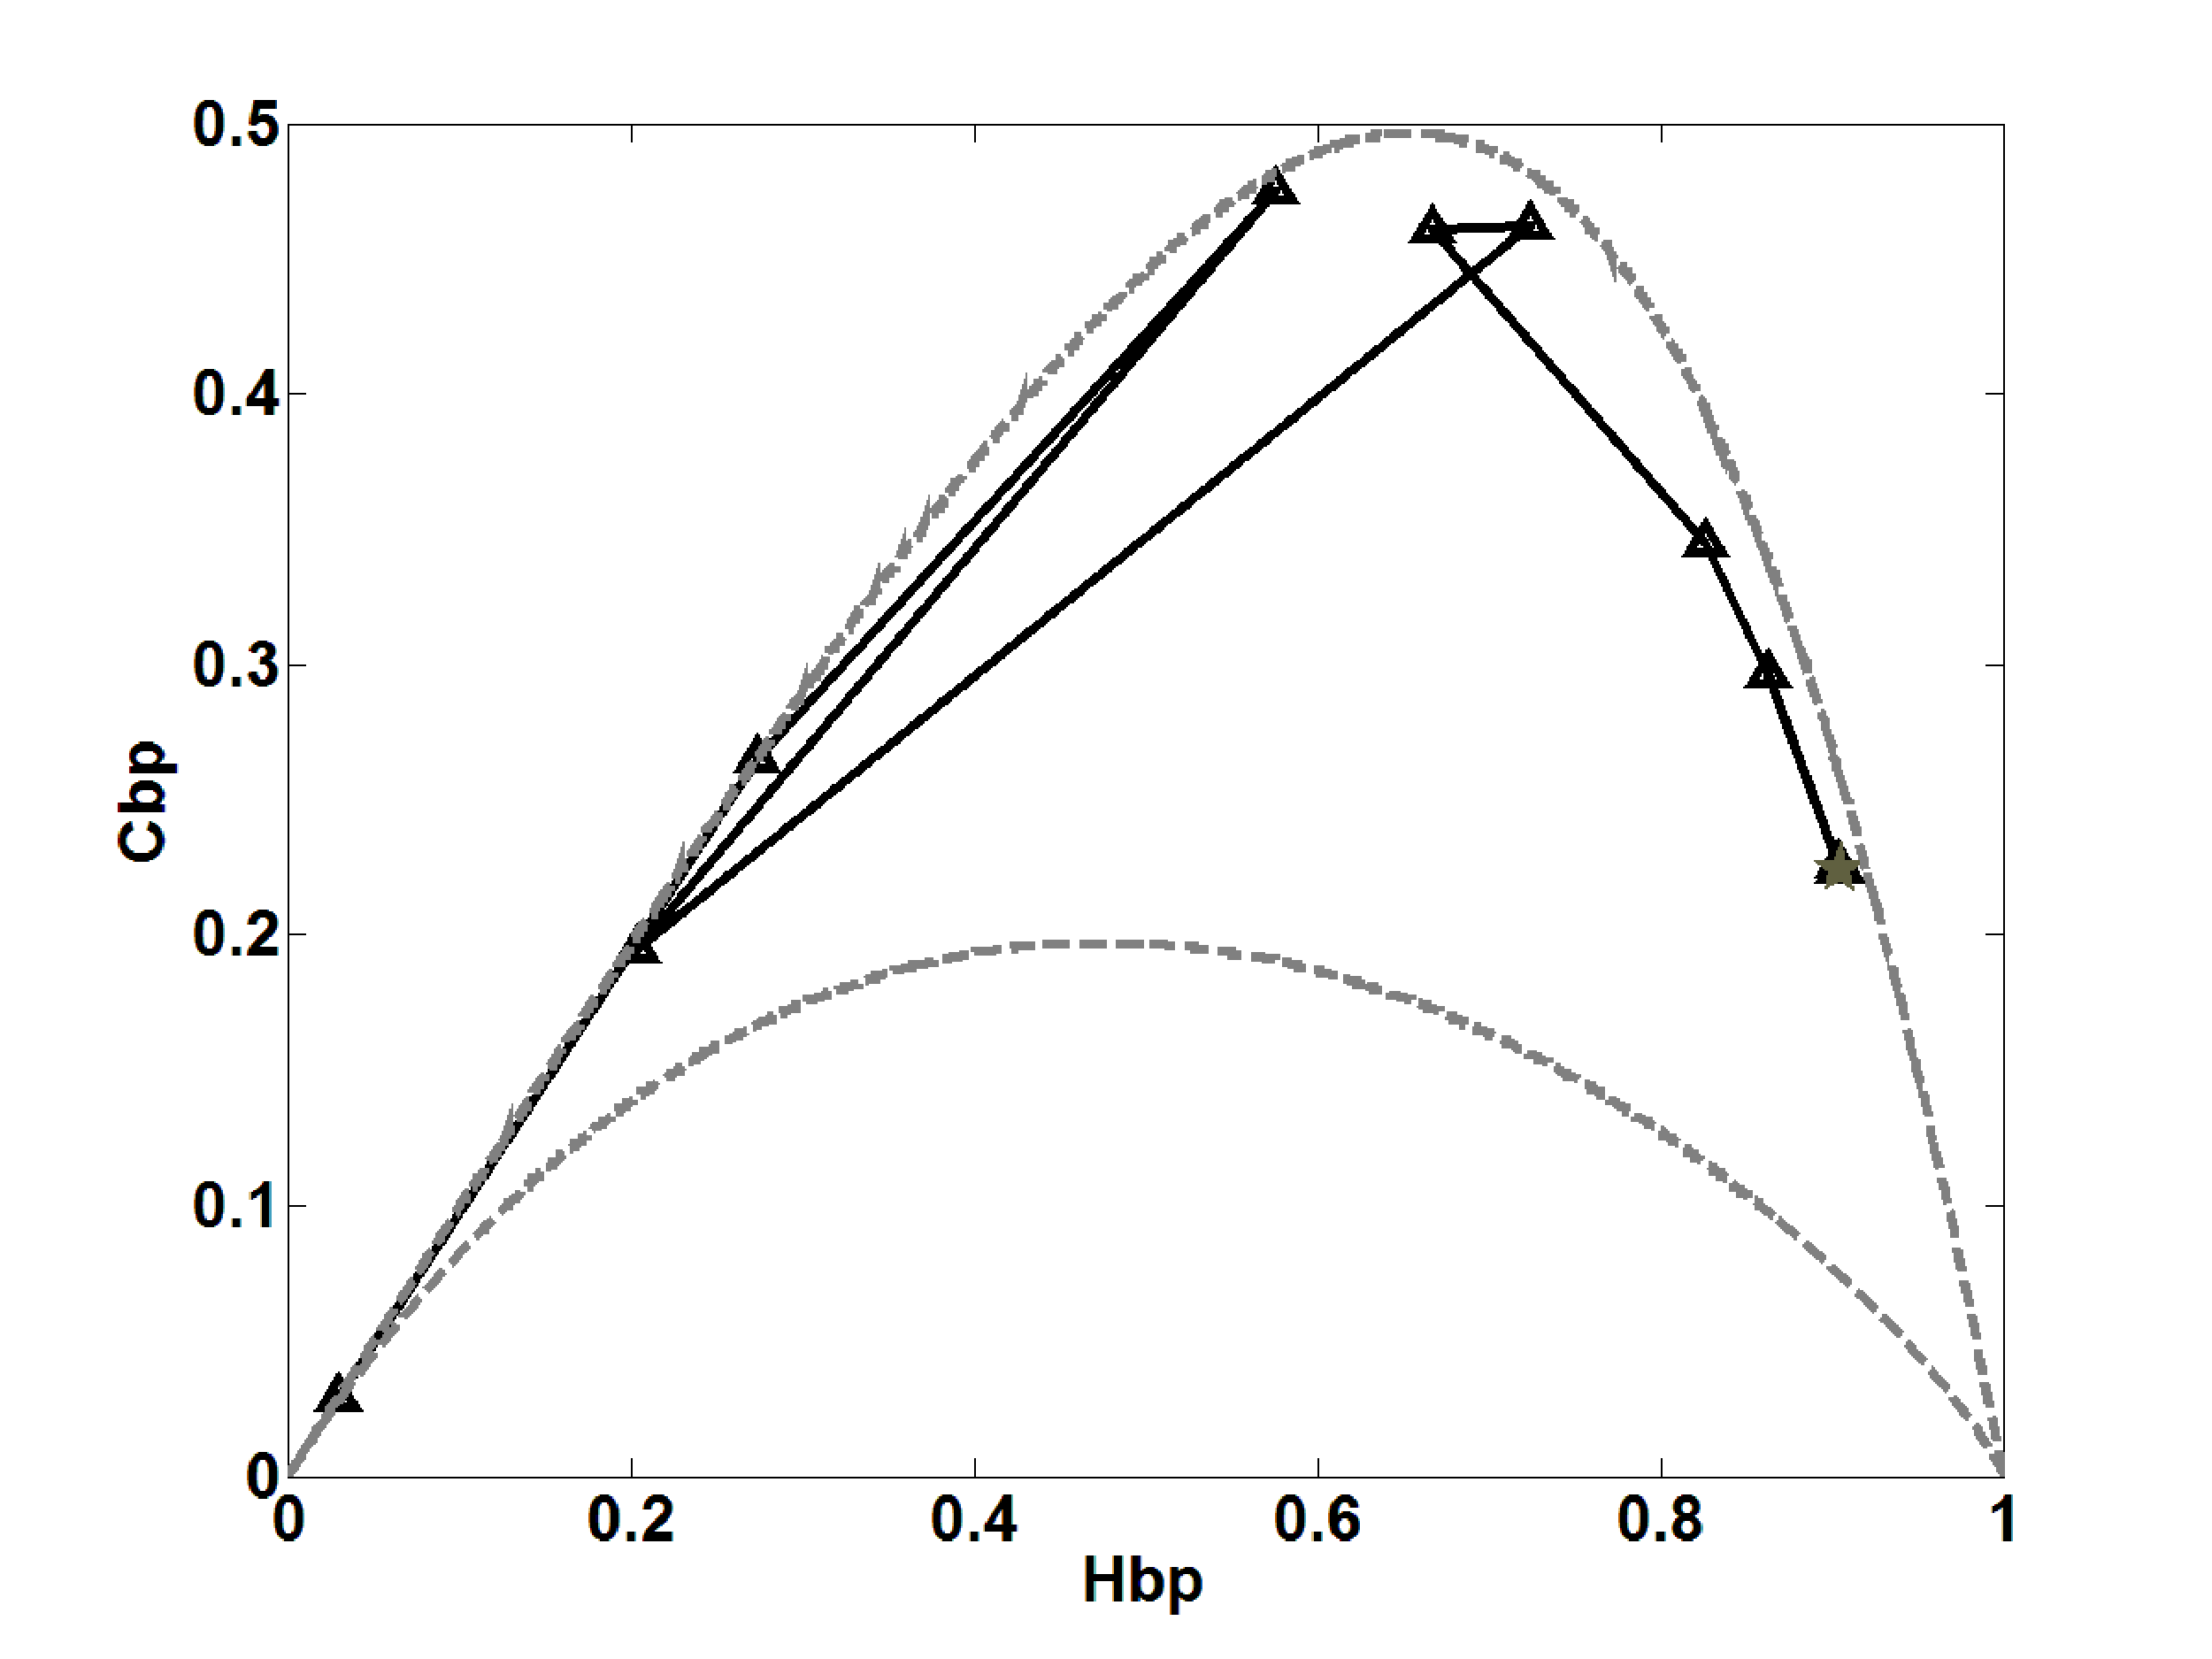
\includegraphics[width=0.3\textwidth]{HbpCbp_parB10}
\caption{Statistical properties of EVEN, obtained by skipping the values in the odd position of the time series of  SWITCH,  using decimal representation: (a) $H_{hist}$ vs $P$ (b) $H_{BP}$ vs $P$ (c) $C_{BP}$ vs $P$ (d) Number of missing ordering patterns $MP$ vs $P$. In Figures (a) to (d) dashed line correspond to floating point numbers. (e) representation in the $H_{hist},H_{BP}$ plane in the the decimal numerical system.  The star represents the state for floating points numbers. (f) representation in the $H_{BP},C_{BP}$ plane.  The star represents the state for floating points numbers. } \label{fig:seqpardec}
\end{figure}

%%%%%%%%%%%%%%%%%%%%%%%%%%%%%%Fig 8.
\begin{figure}
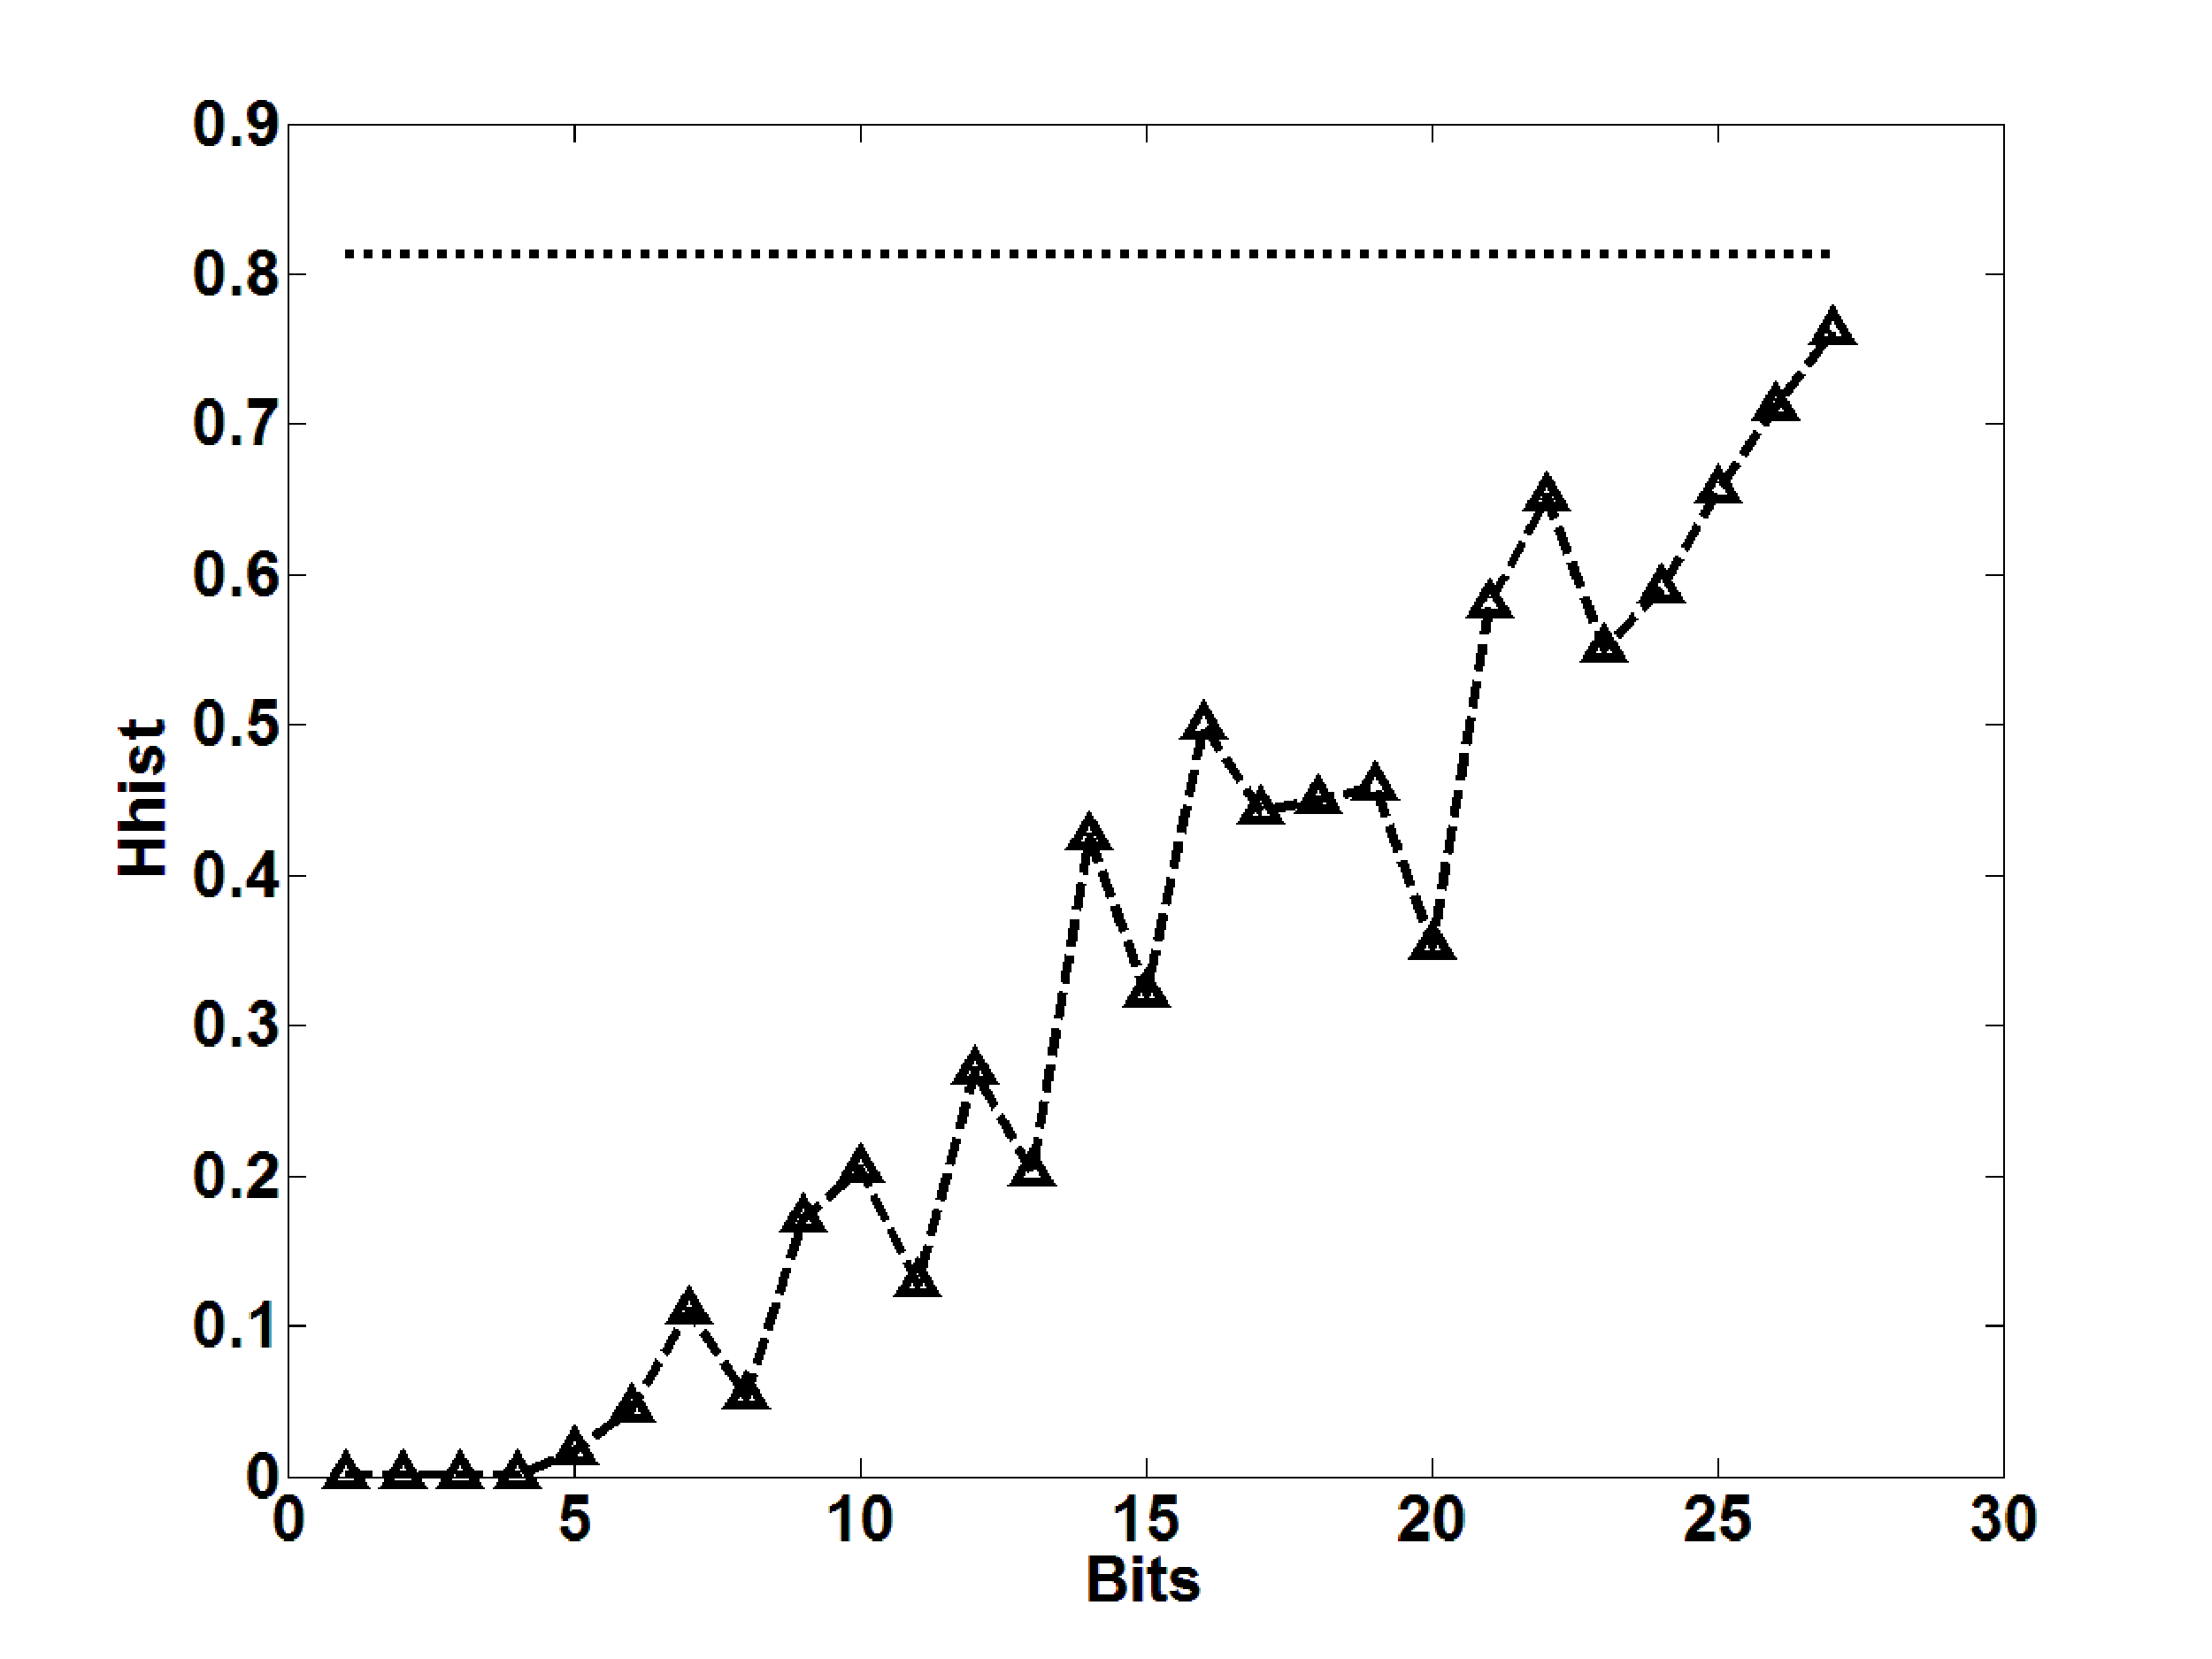
\includegraphics[width=0.3\textwidth]{Hhist_parB2}
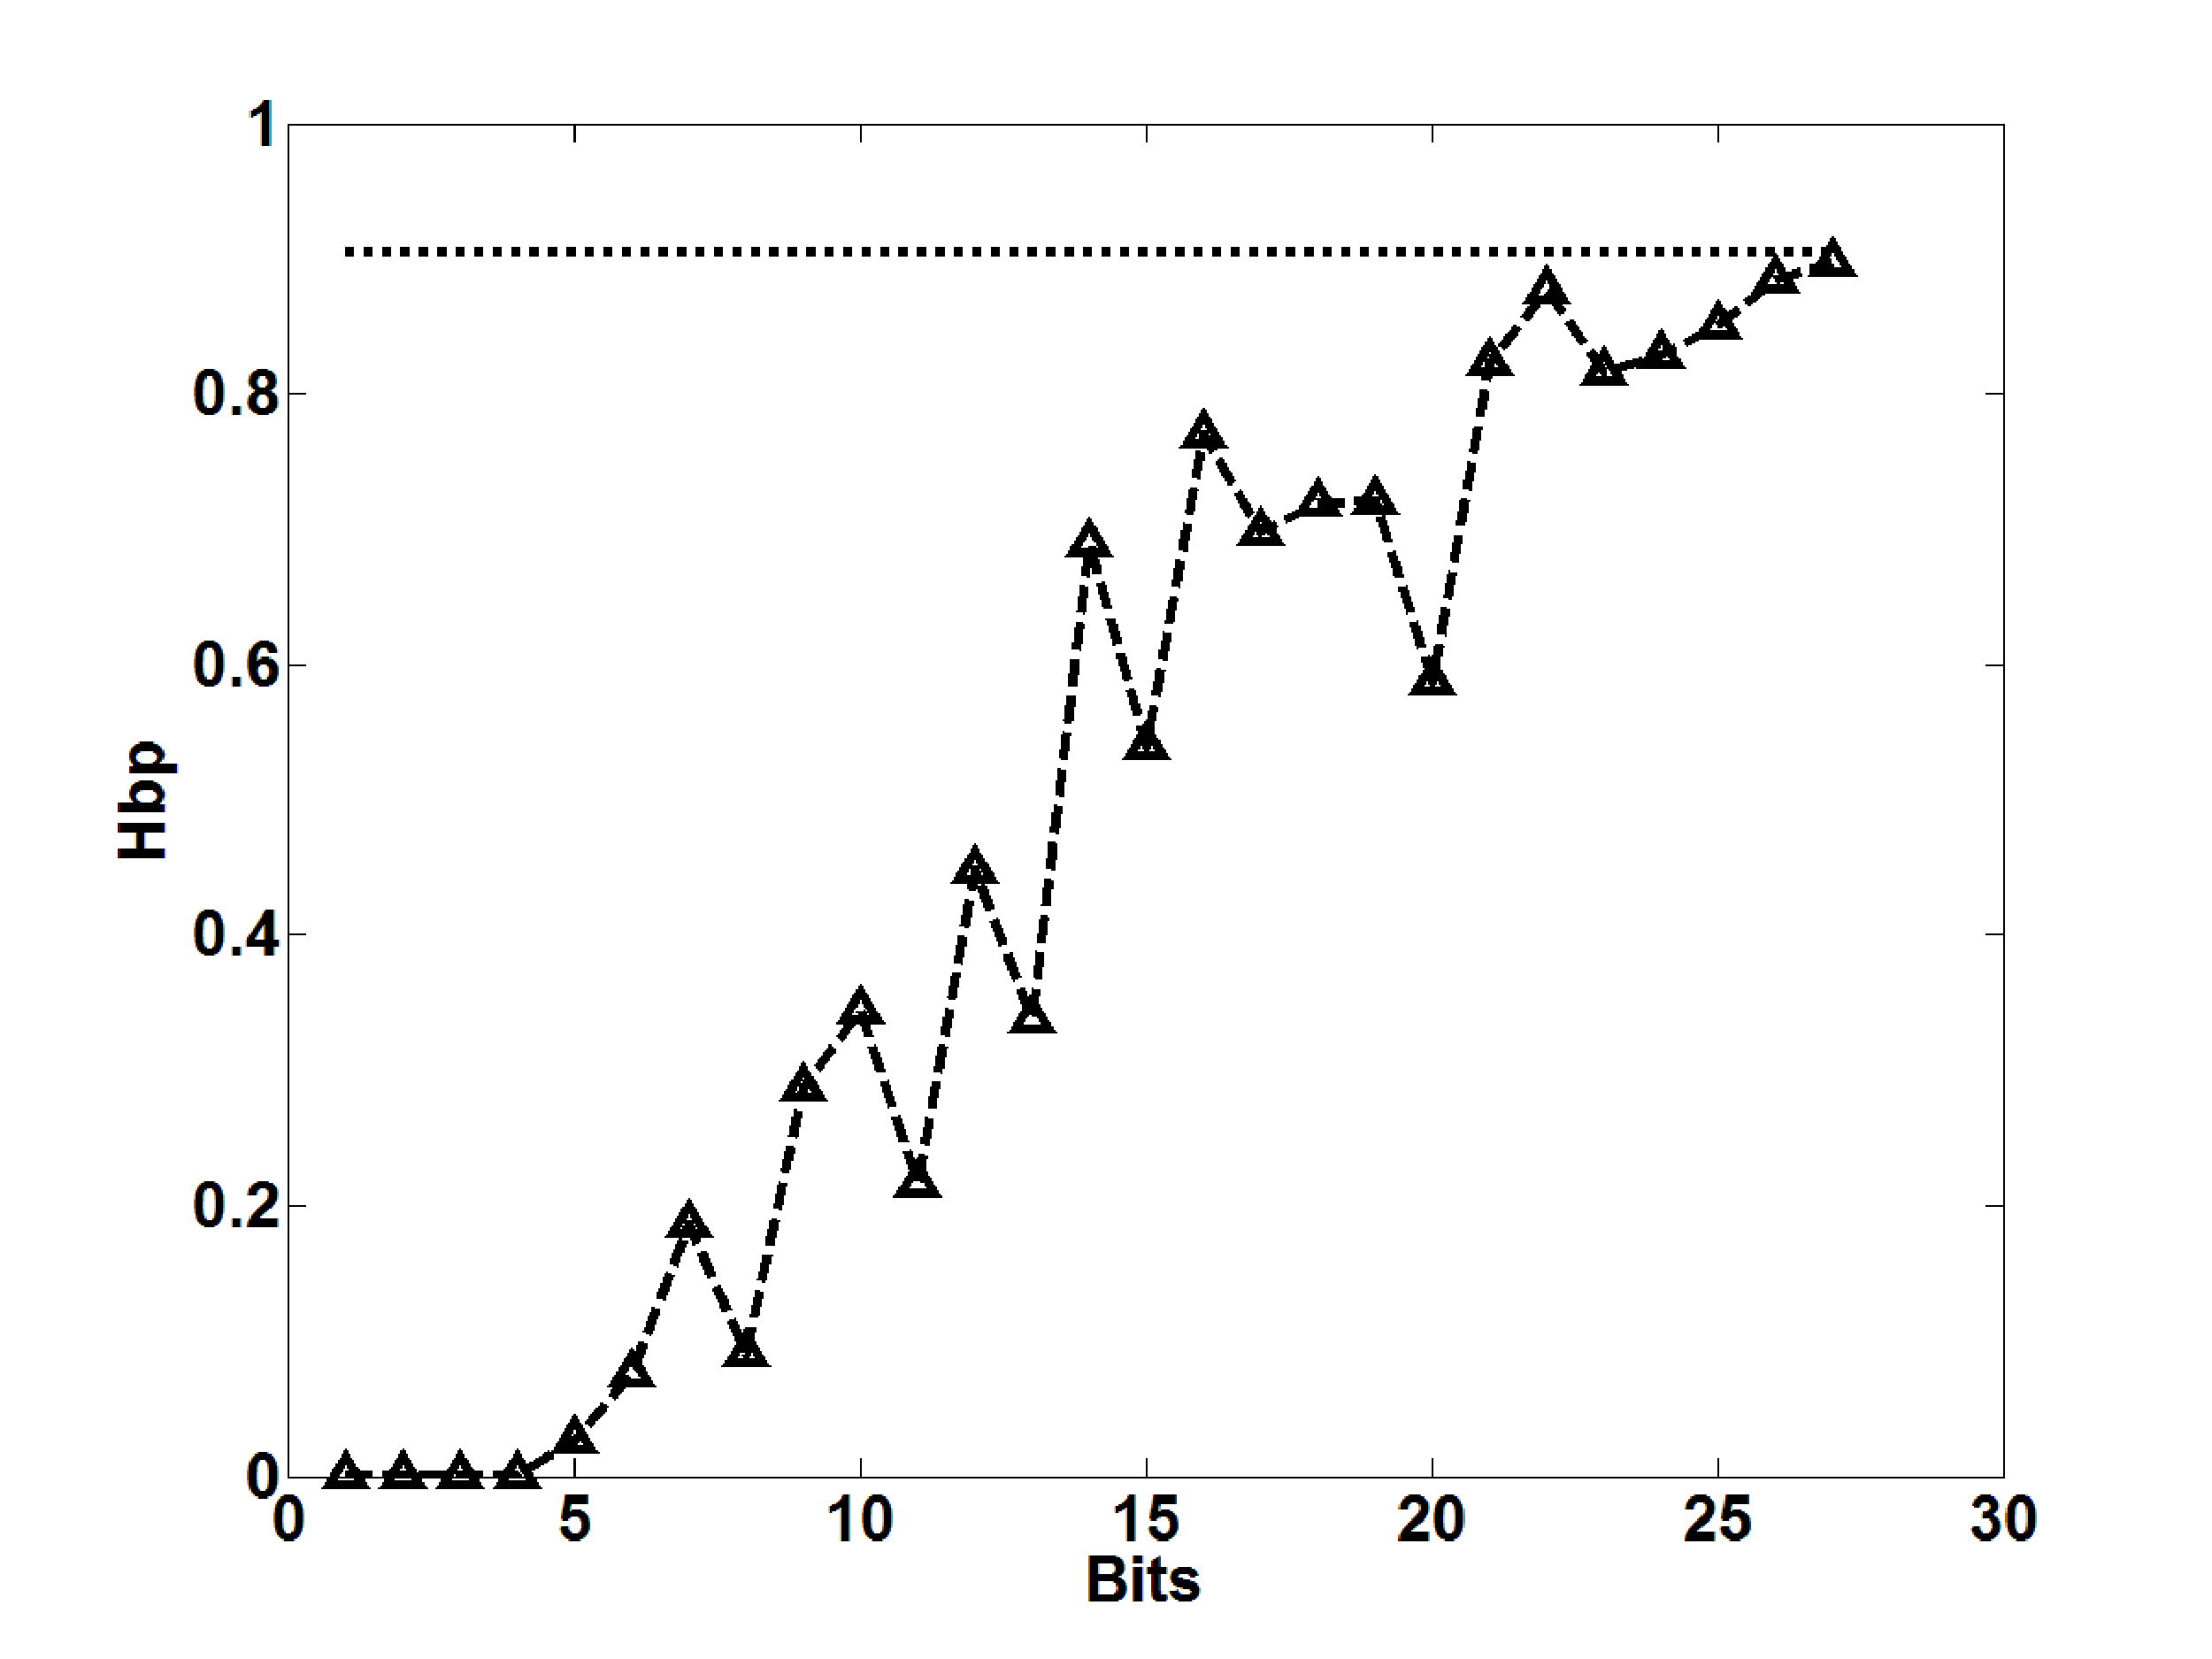
\includegraphics[width=0.3\textwidth]{Hbp_parB2}
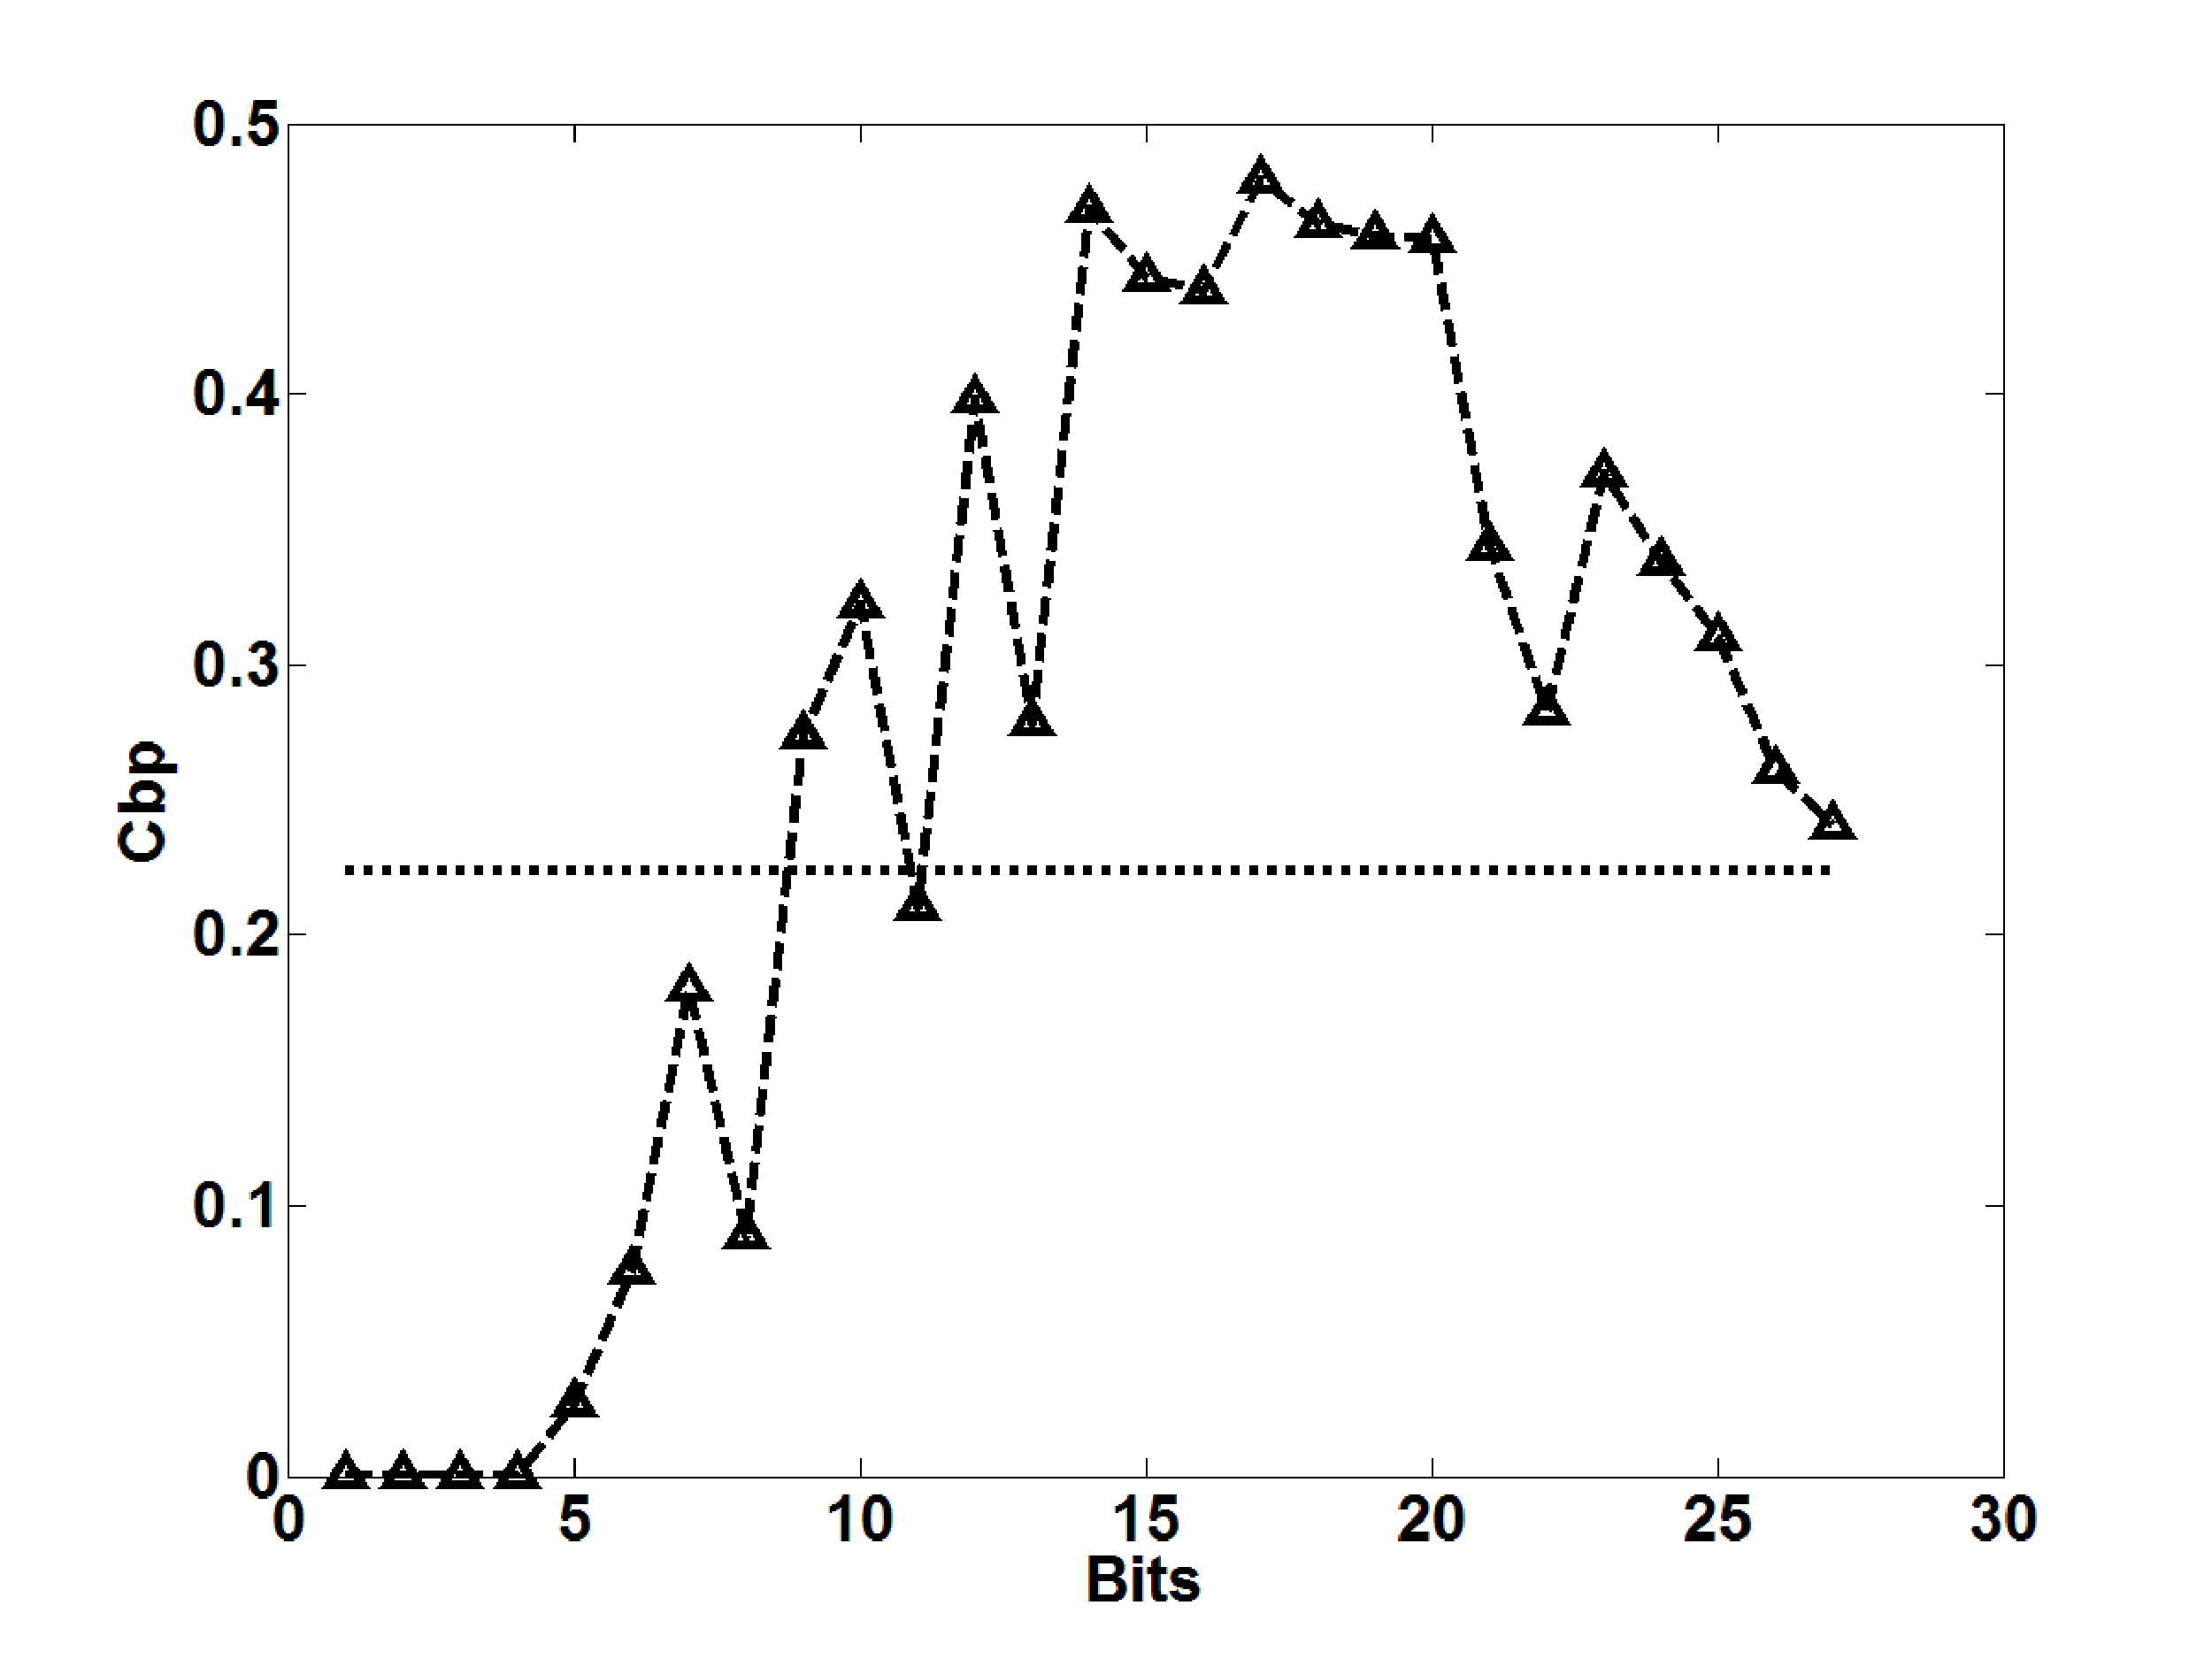
\includegraphics[width=0.3\textwidth]{Cbp_parB2}
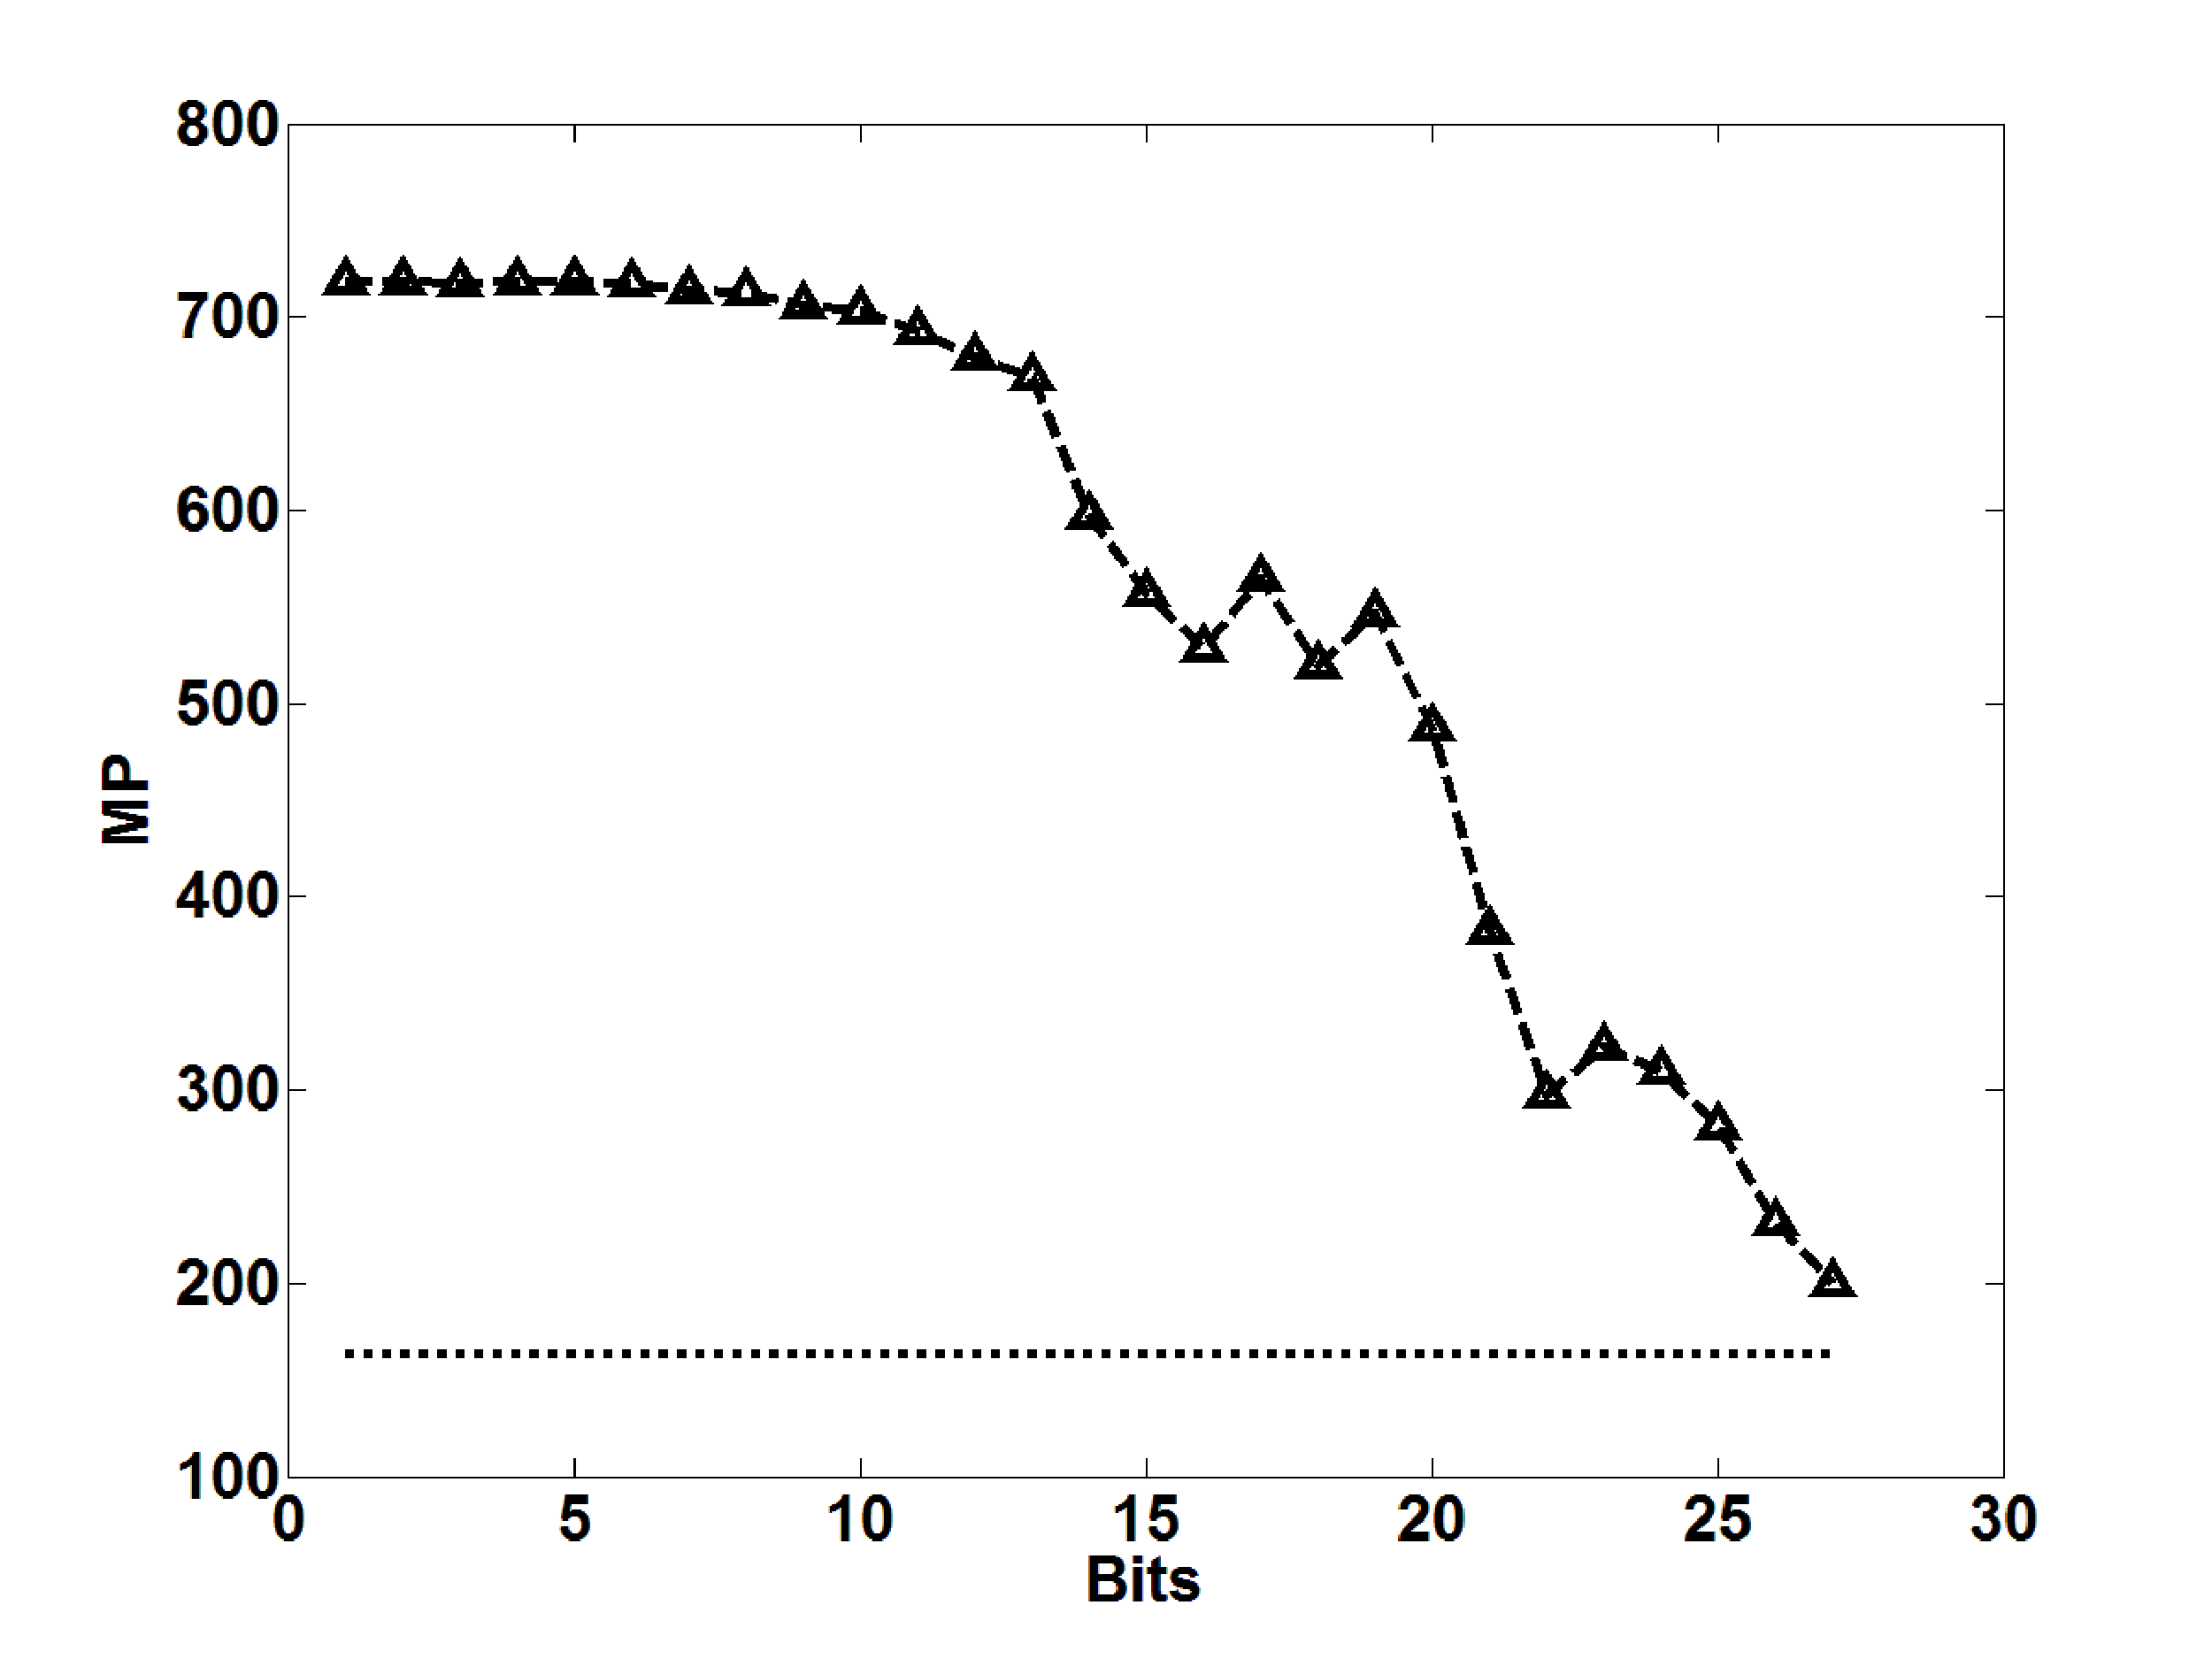
\includegraphics[width=0.3\textwidth]{Miss_parB2}
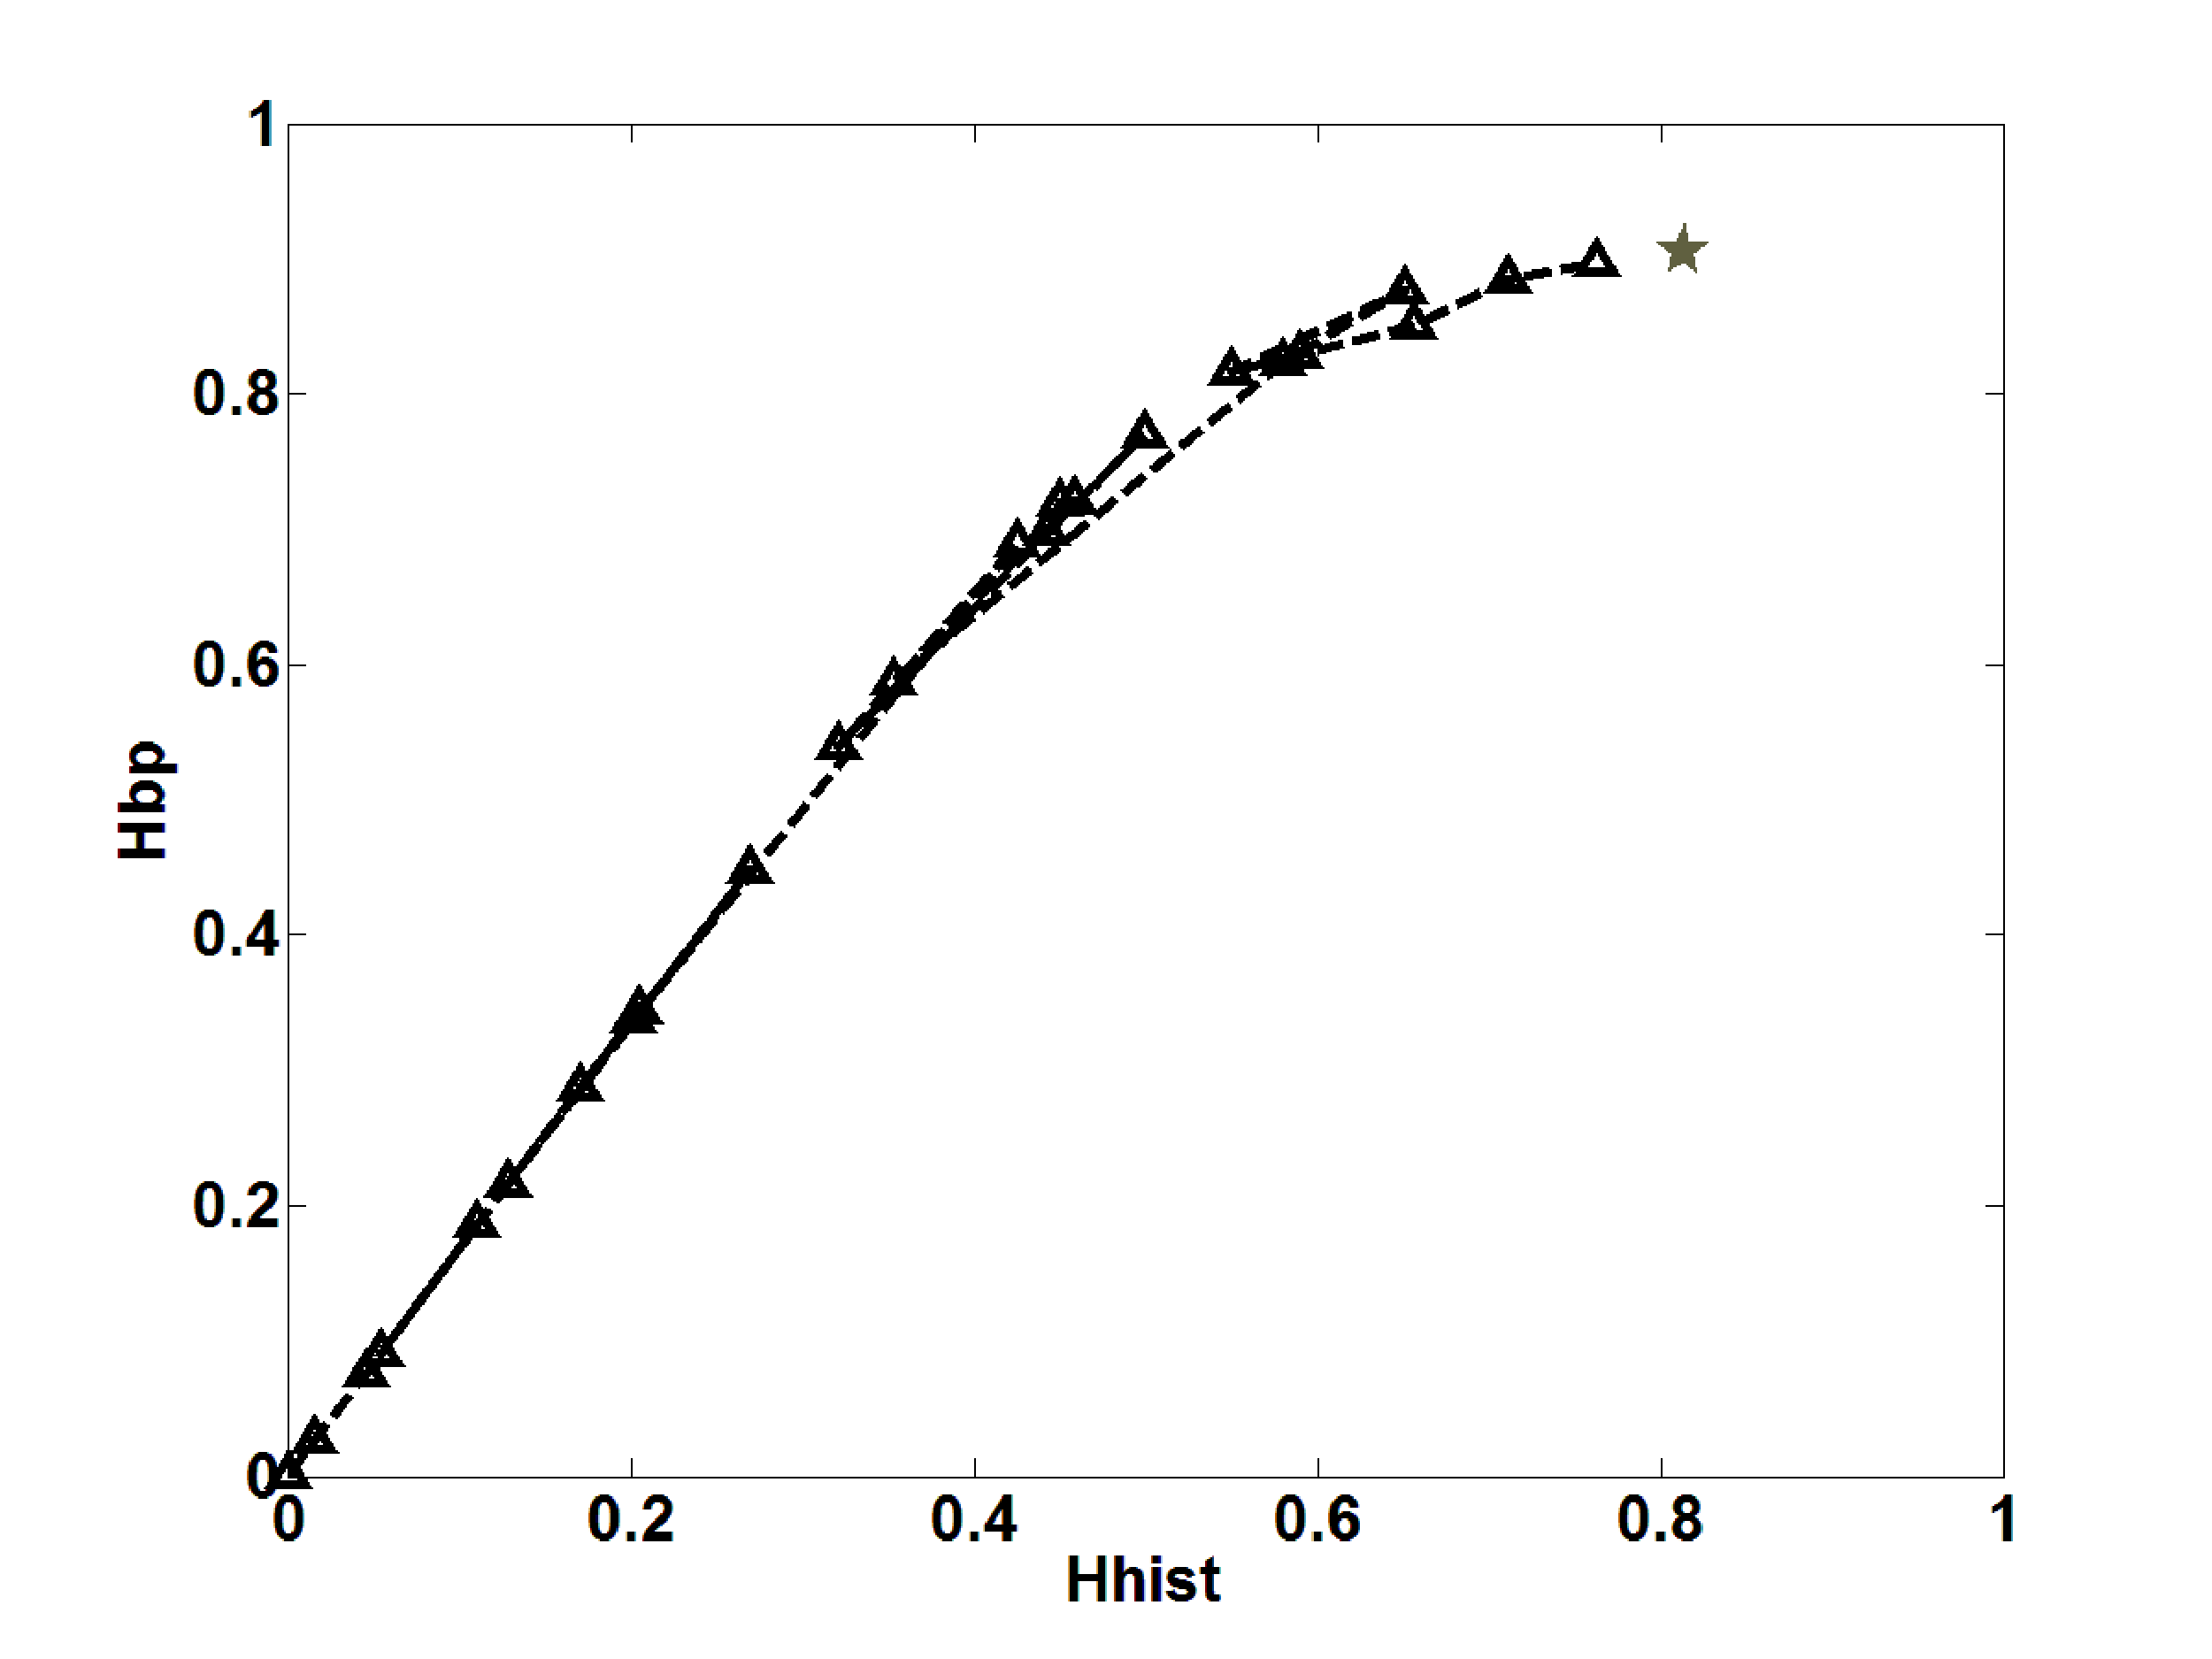
\includegraphics[width=0.3\textwidth]{HhistHbp_parB2}
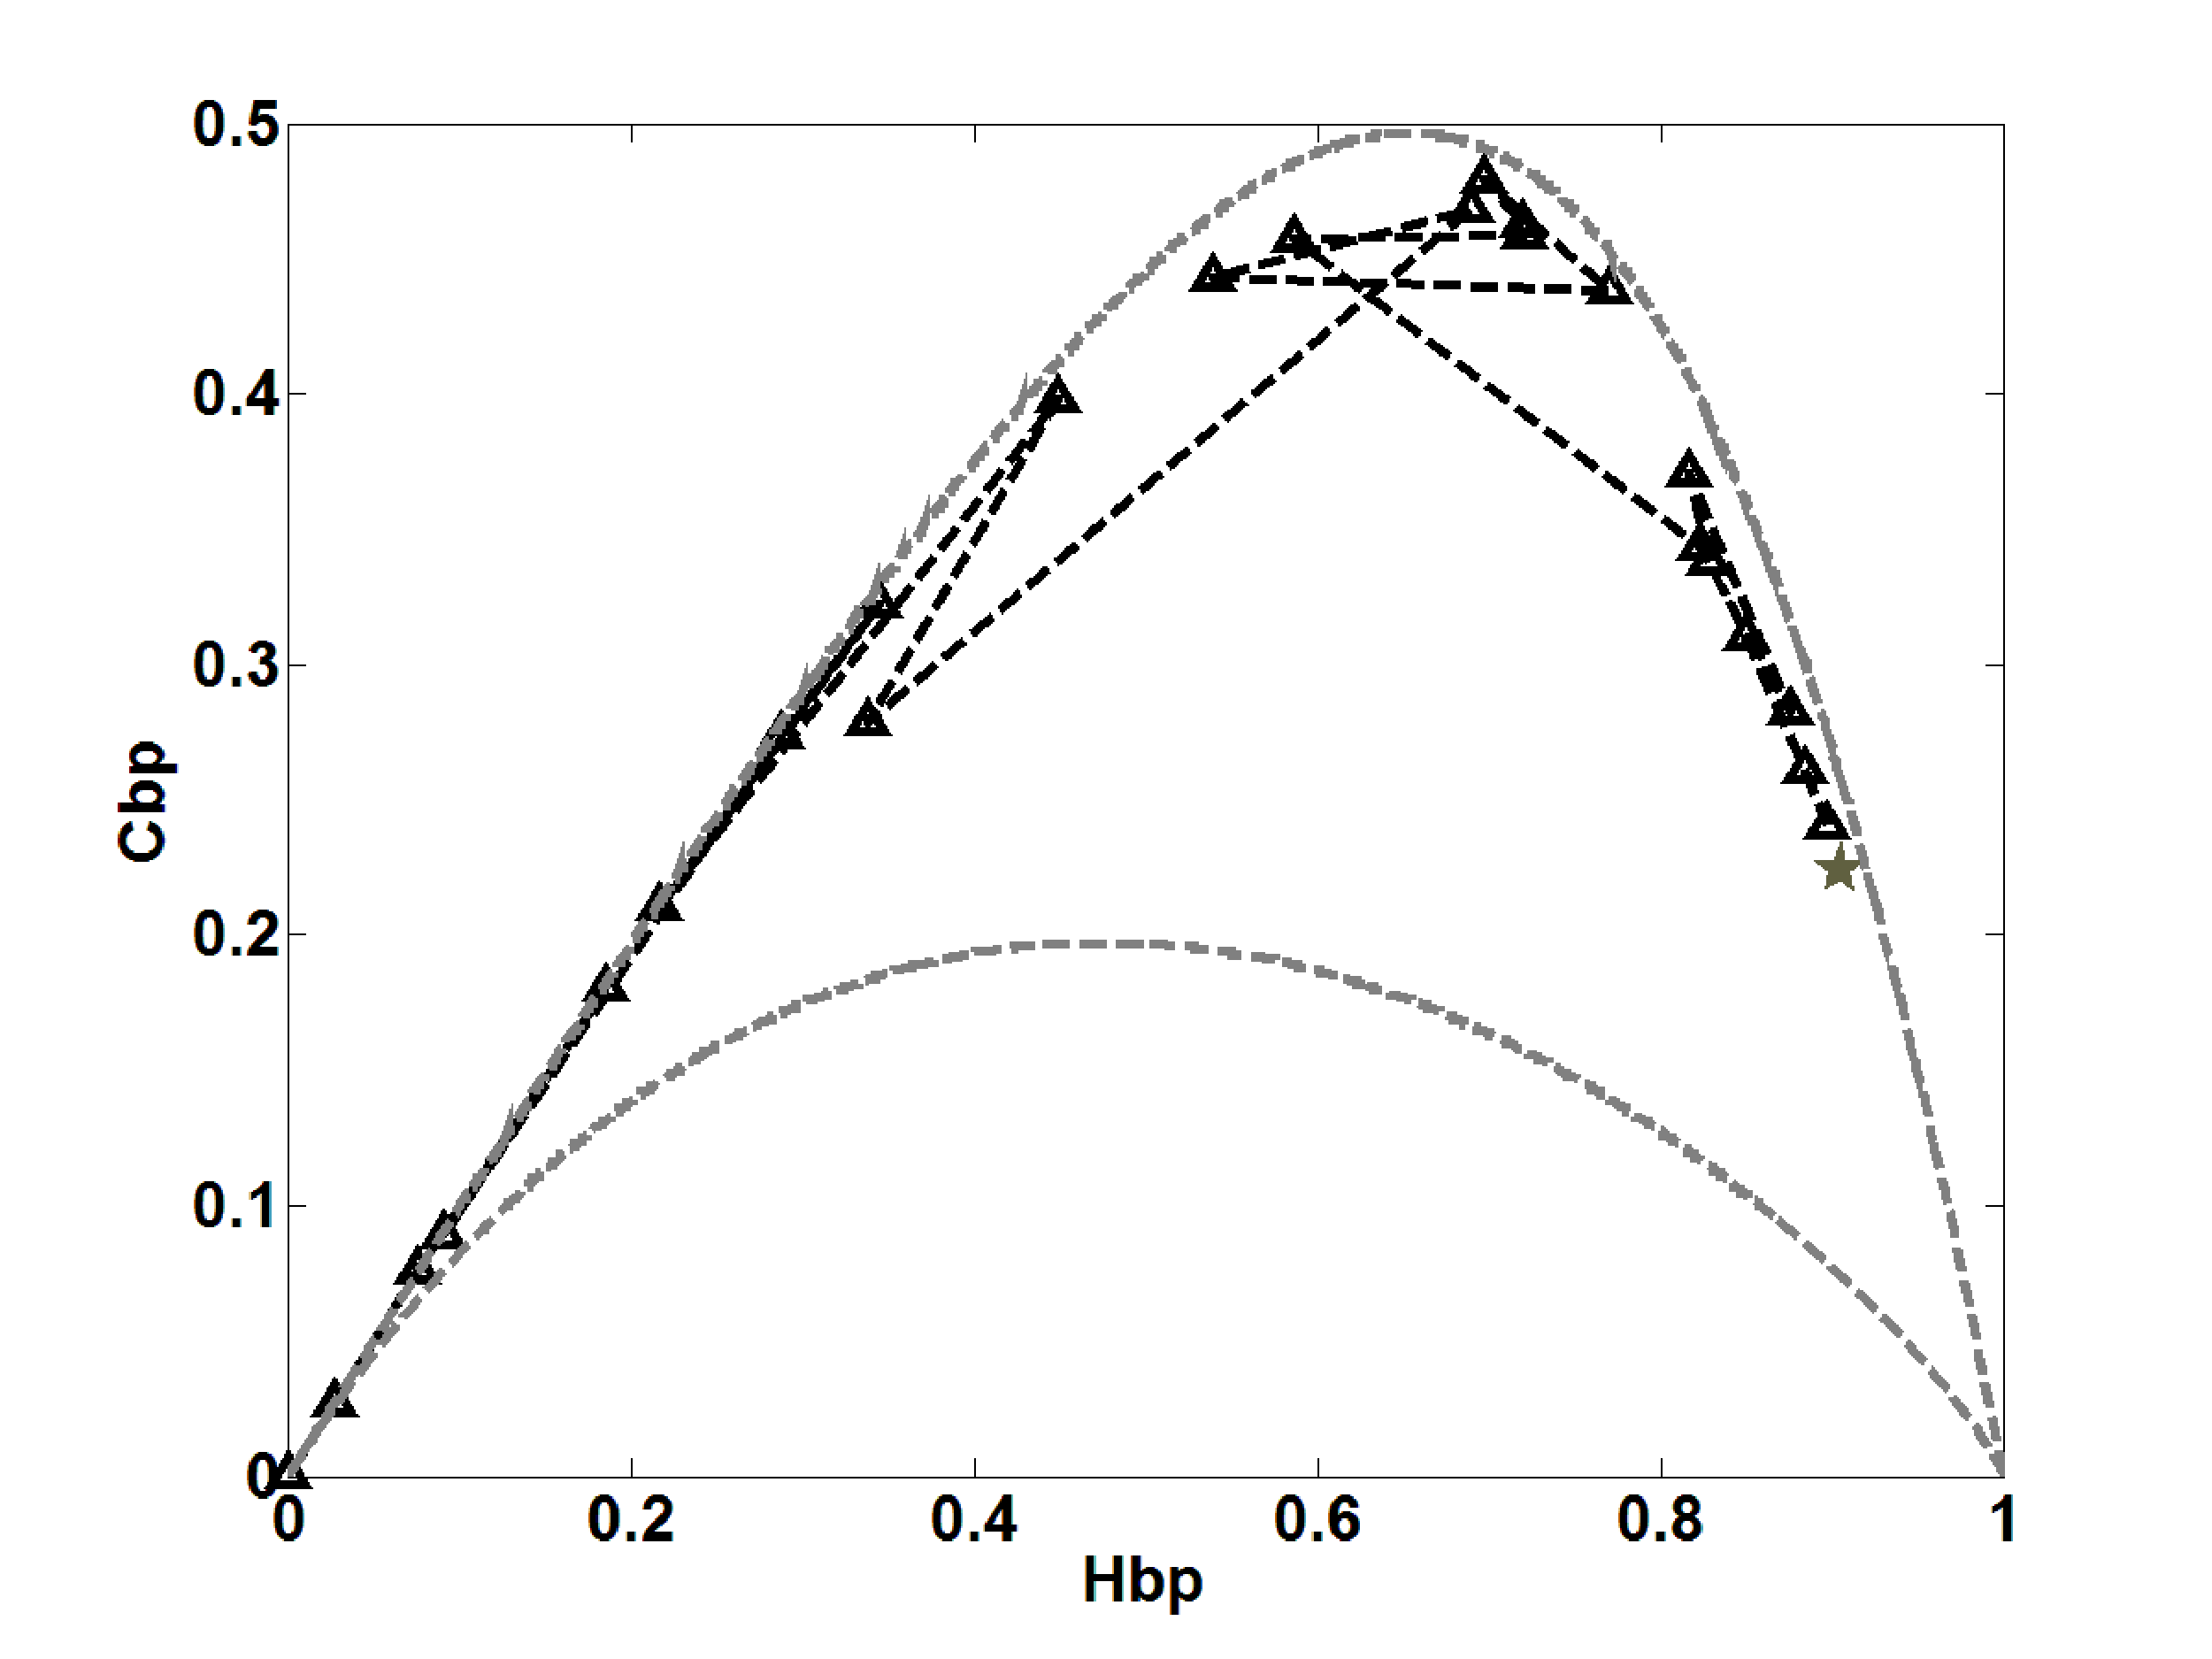
\includegraphics[width=0.3\textwidth]{HbpCbp_parB2}
\caption{Statistical properties of EVEN, obtained by skipping the values in the odd position of the time series of  SWITCH,  using binary representation: (a) $H_{hist}$ vs $P$ (b) $H_{BP}$ vs $P$ (c) $C_{BP}$ vs $P$ (d) Number of missing ordering patterns $MP$ vs $P$. In Figures (a) to (d) dashed line correspond to floating point numbers. (e) representation in the $H_{hist},H_{BP}$ plane in the the binary numerical system.  The star represents the state for floating points numbers. (f) representation in the $H_{BP},C_{BP}$ plane.  The star represents the state for floating points numbers.  } \label{fig:seqparbin}
\end{figure}

%%%%%%%%%%%%%%%%%%%%%%%%%%
%%%%%%%%%%%%%%%%%%%%%%%%%%%% Fig.9
%\begin{figure}
%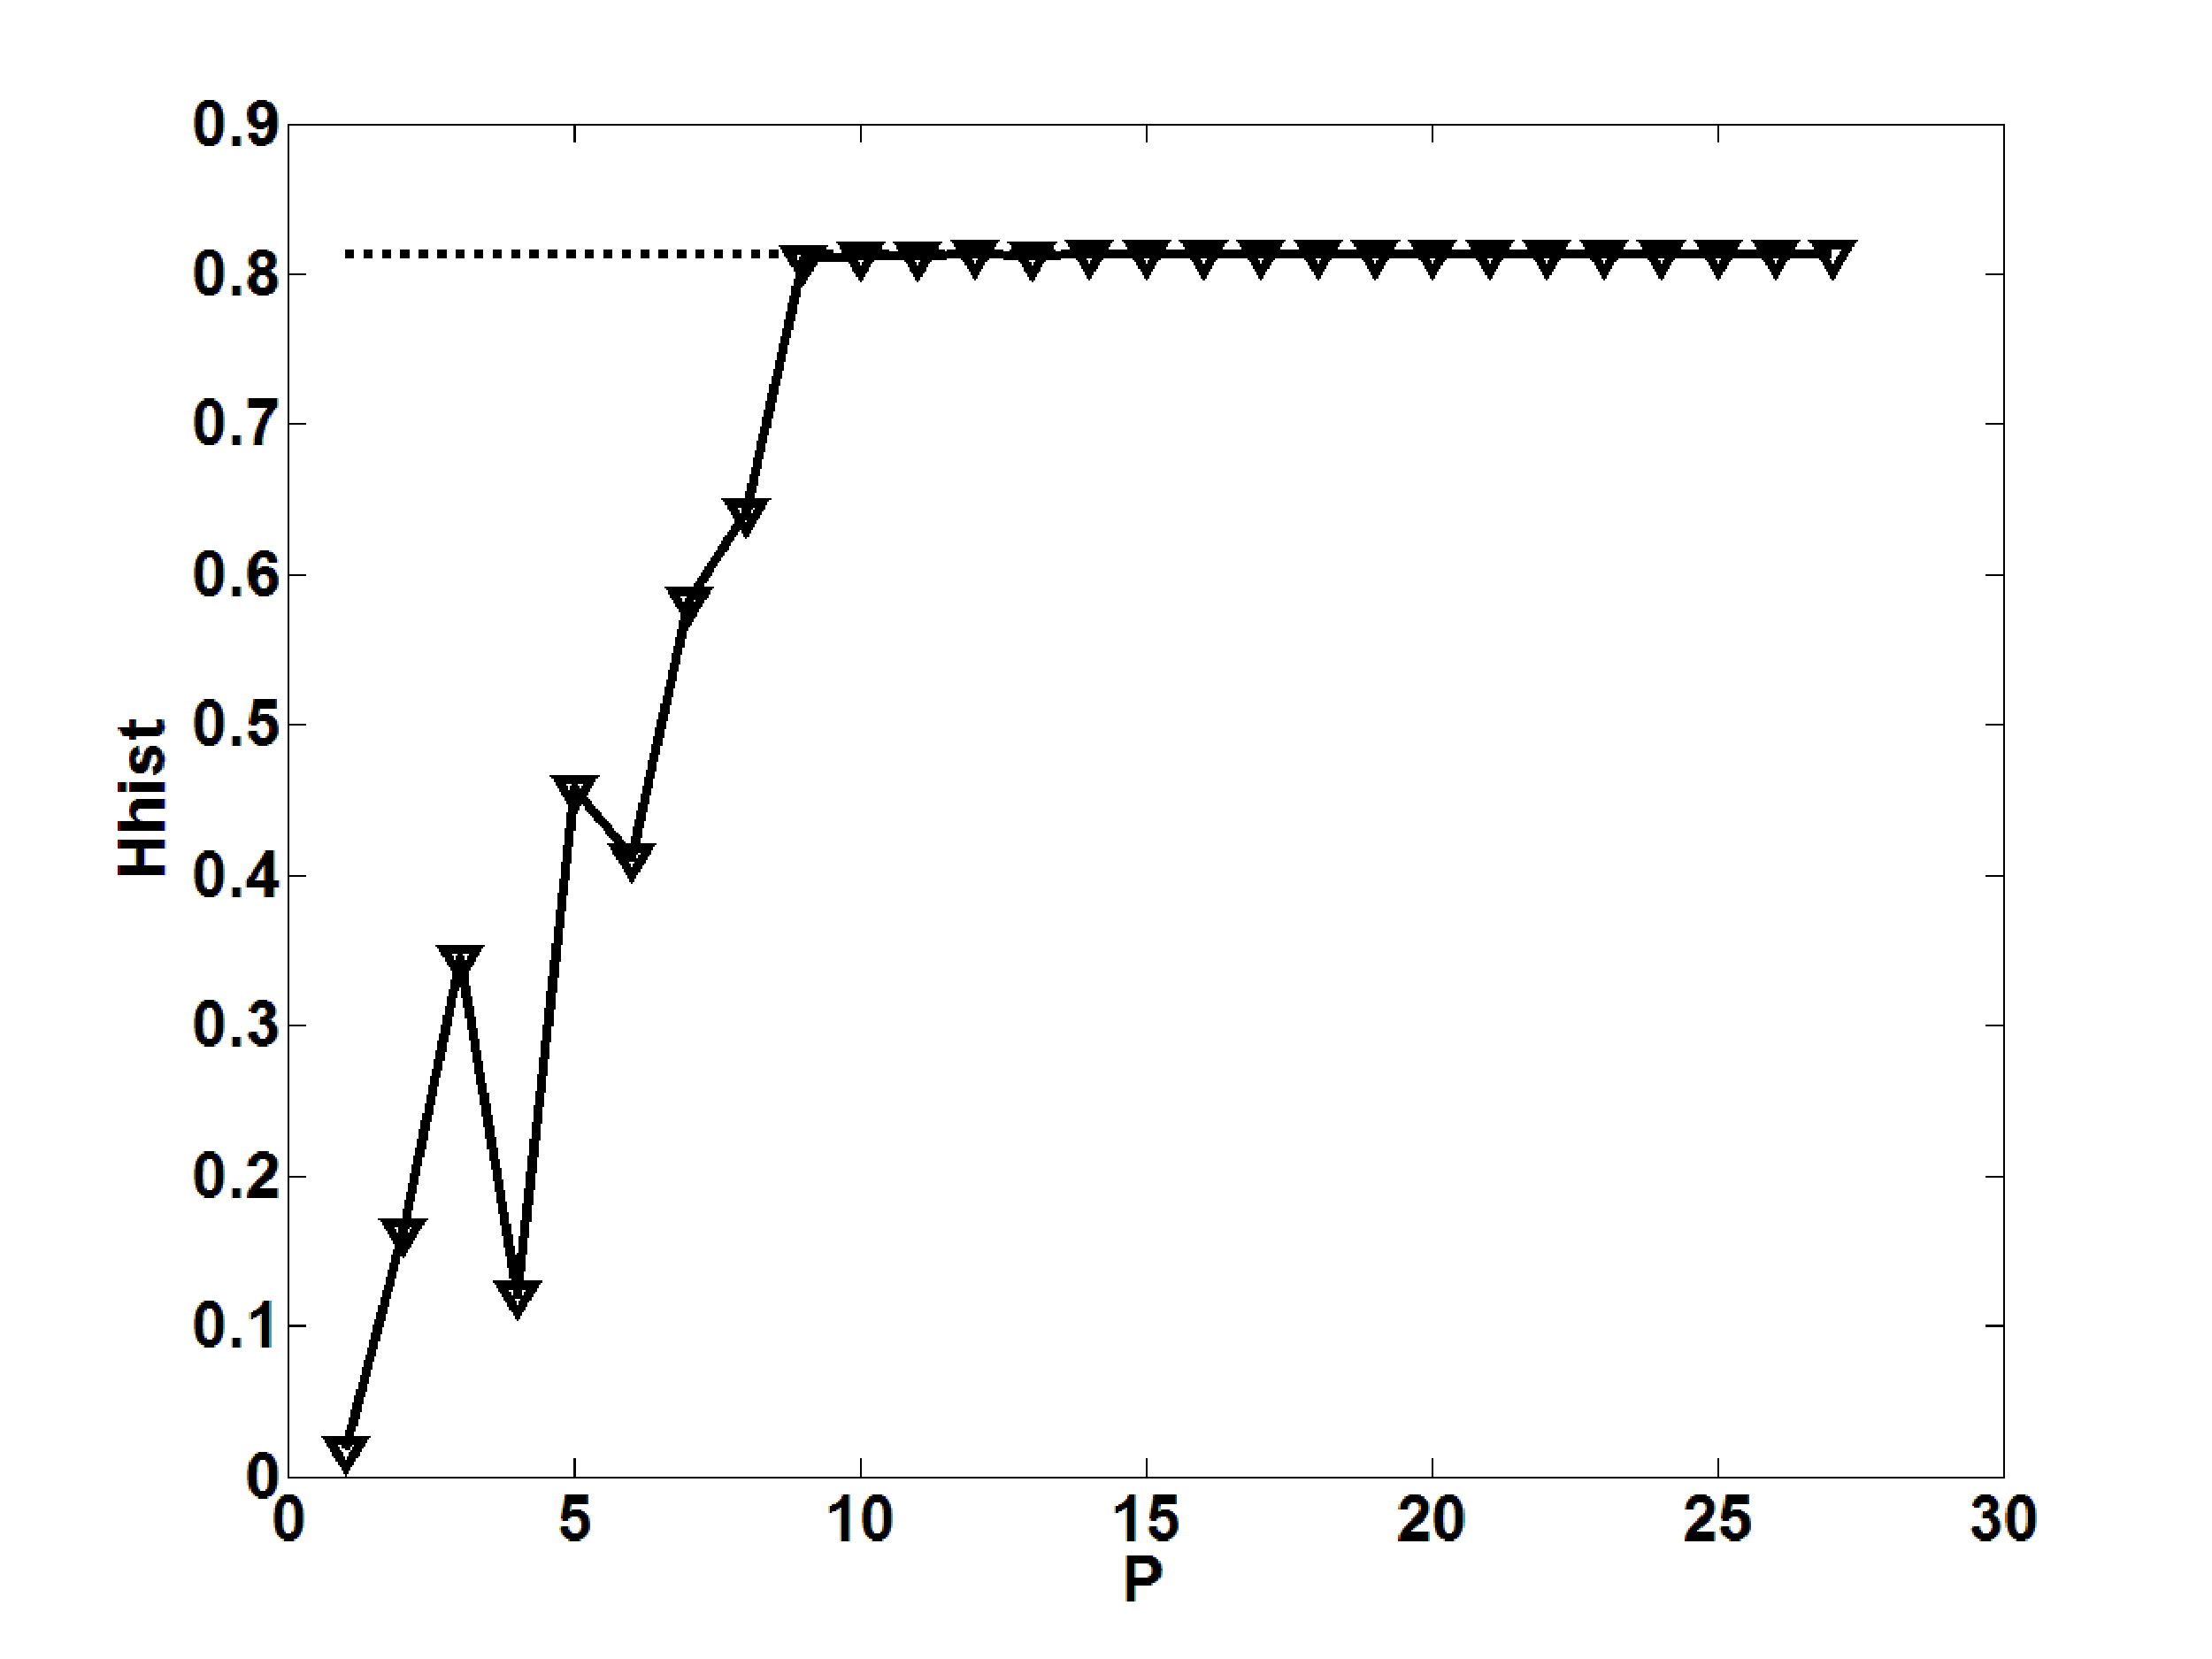
\includegraphics[width=0.3\textwidth]{Hhist_imparB10}
%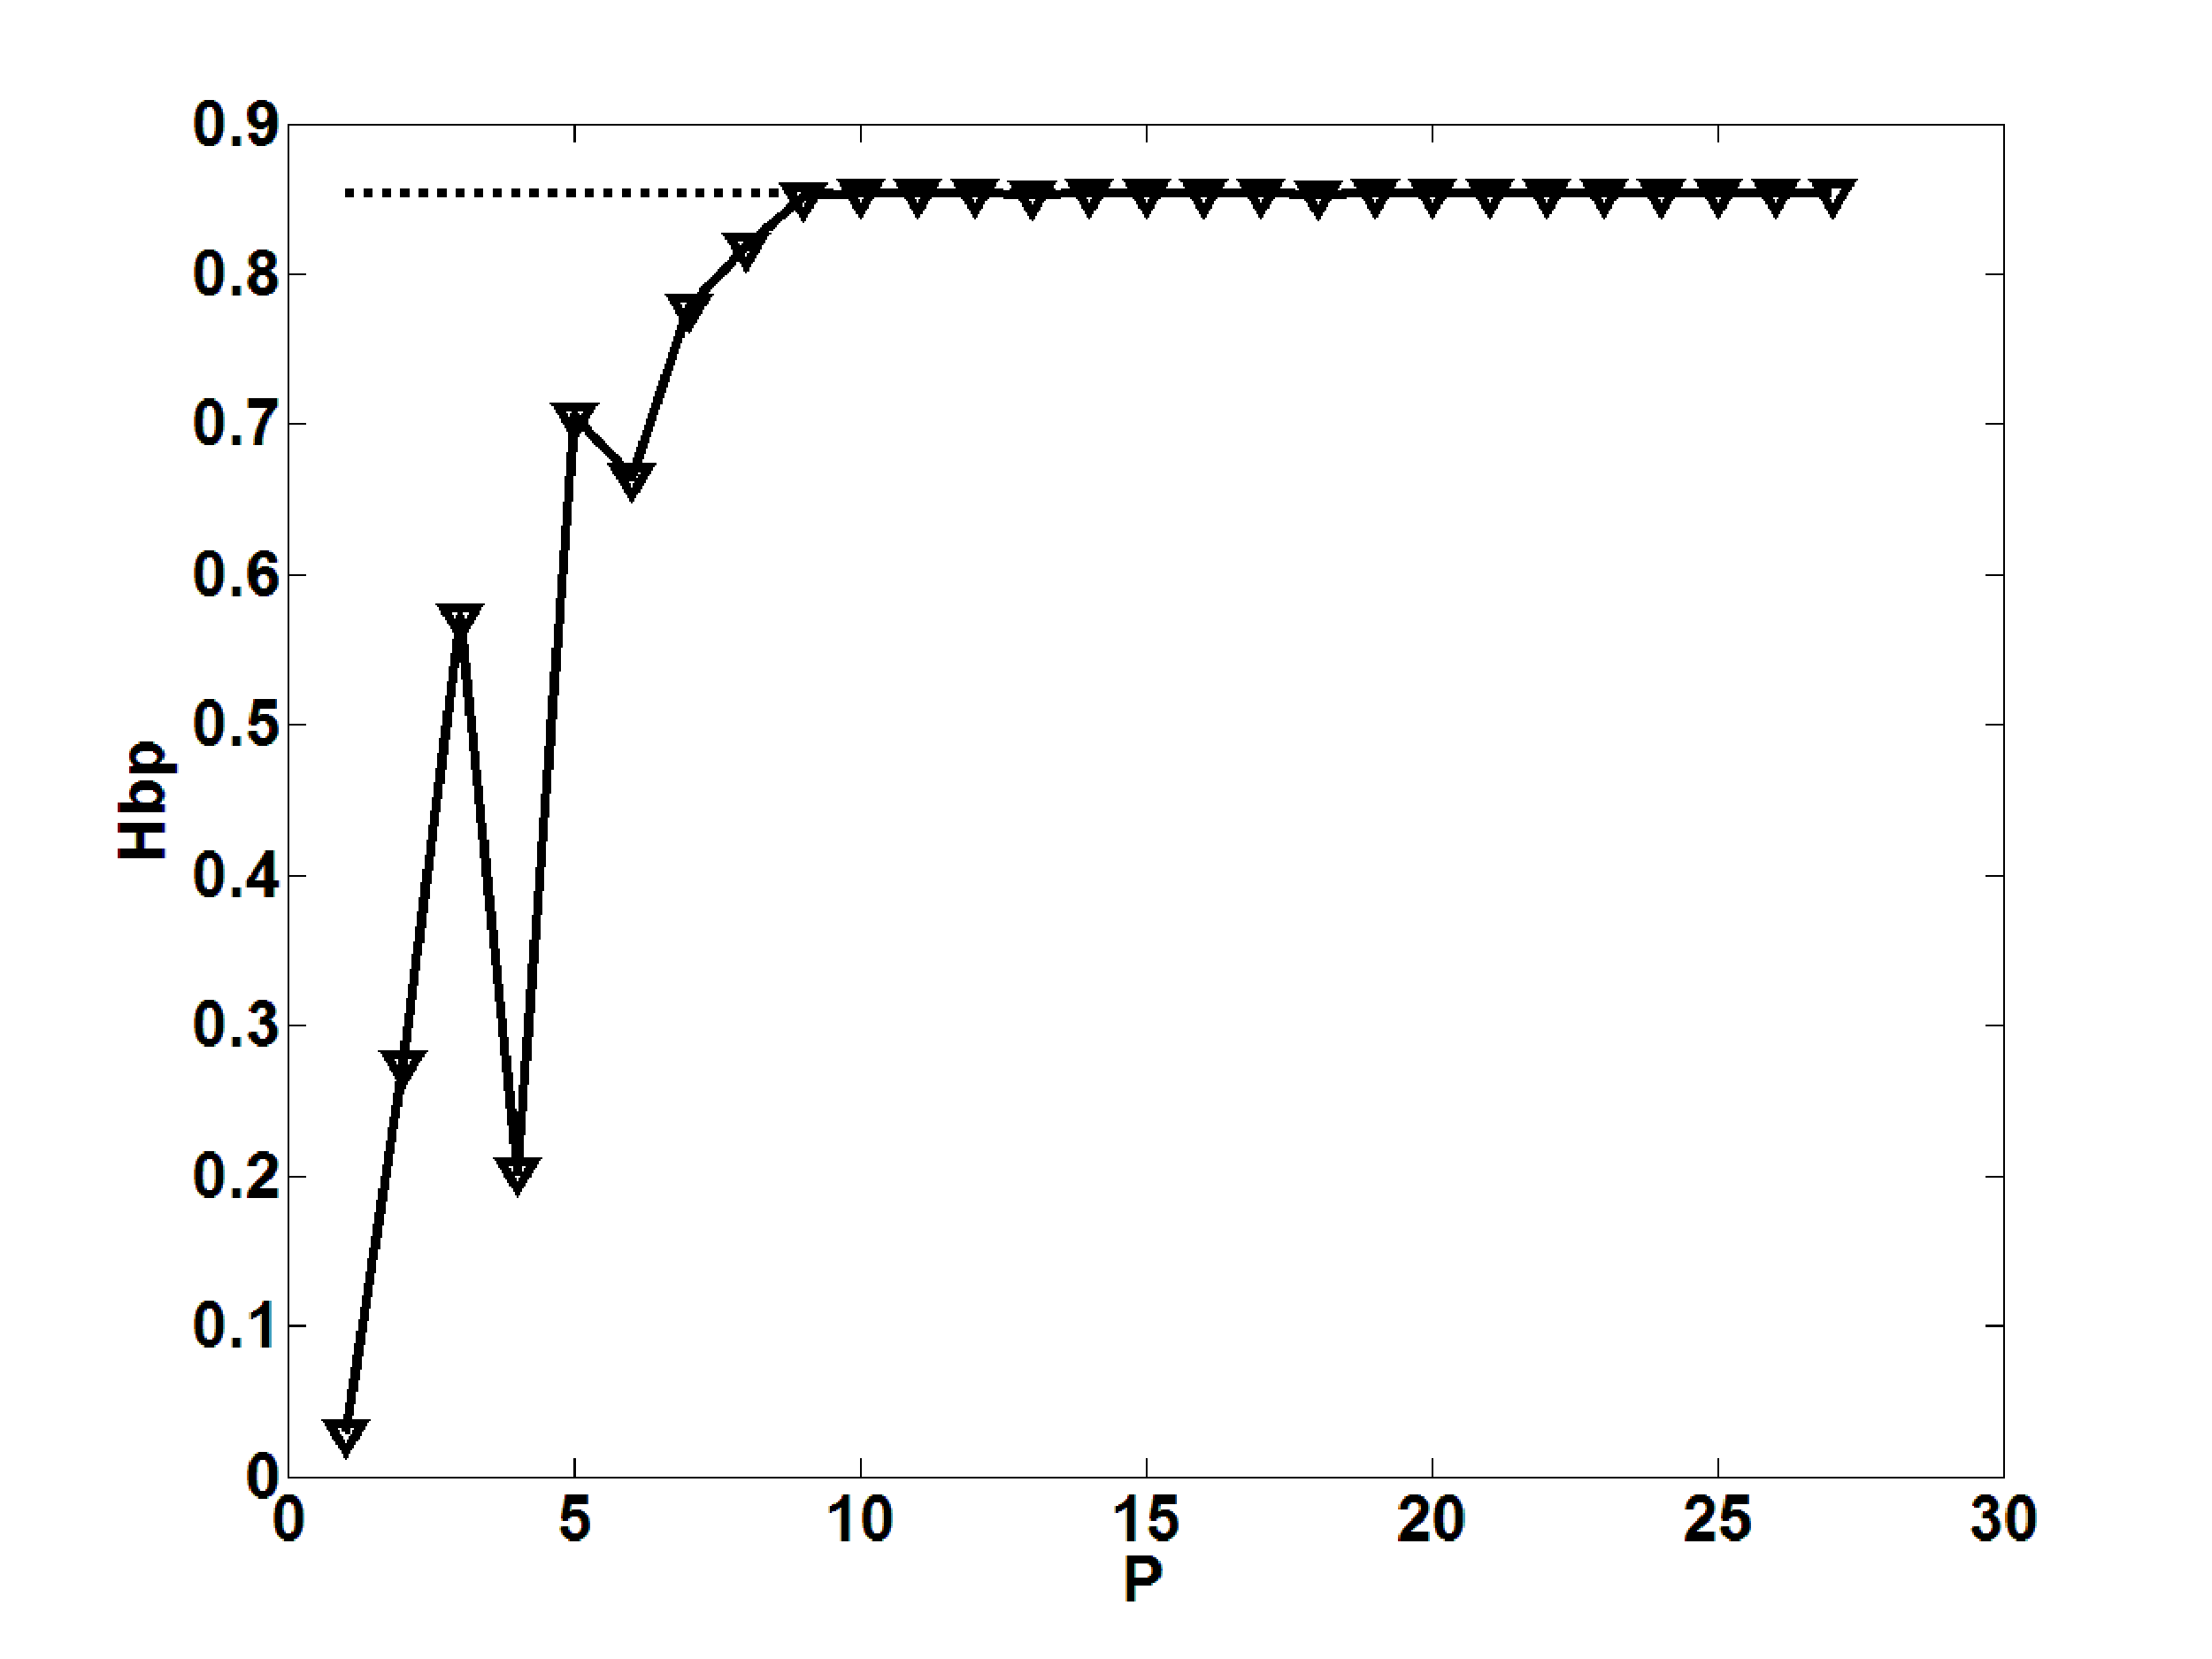
\includegraphics[width=0.3\textwidth]{Hbp_imparB10}
%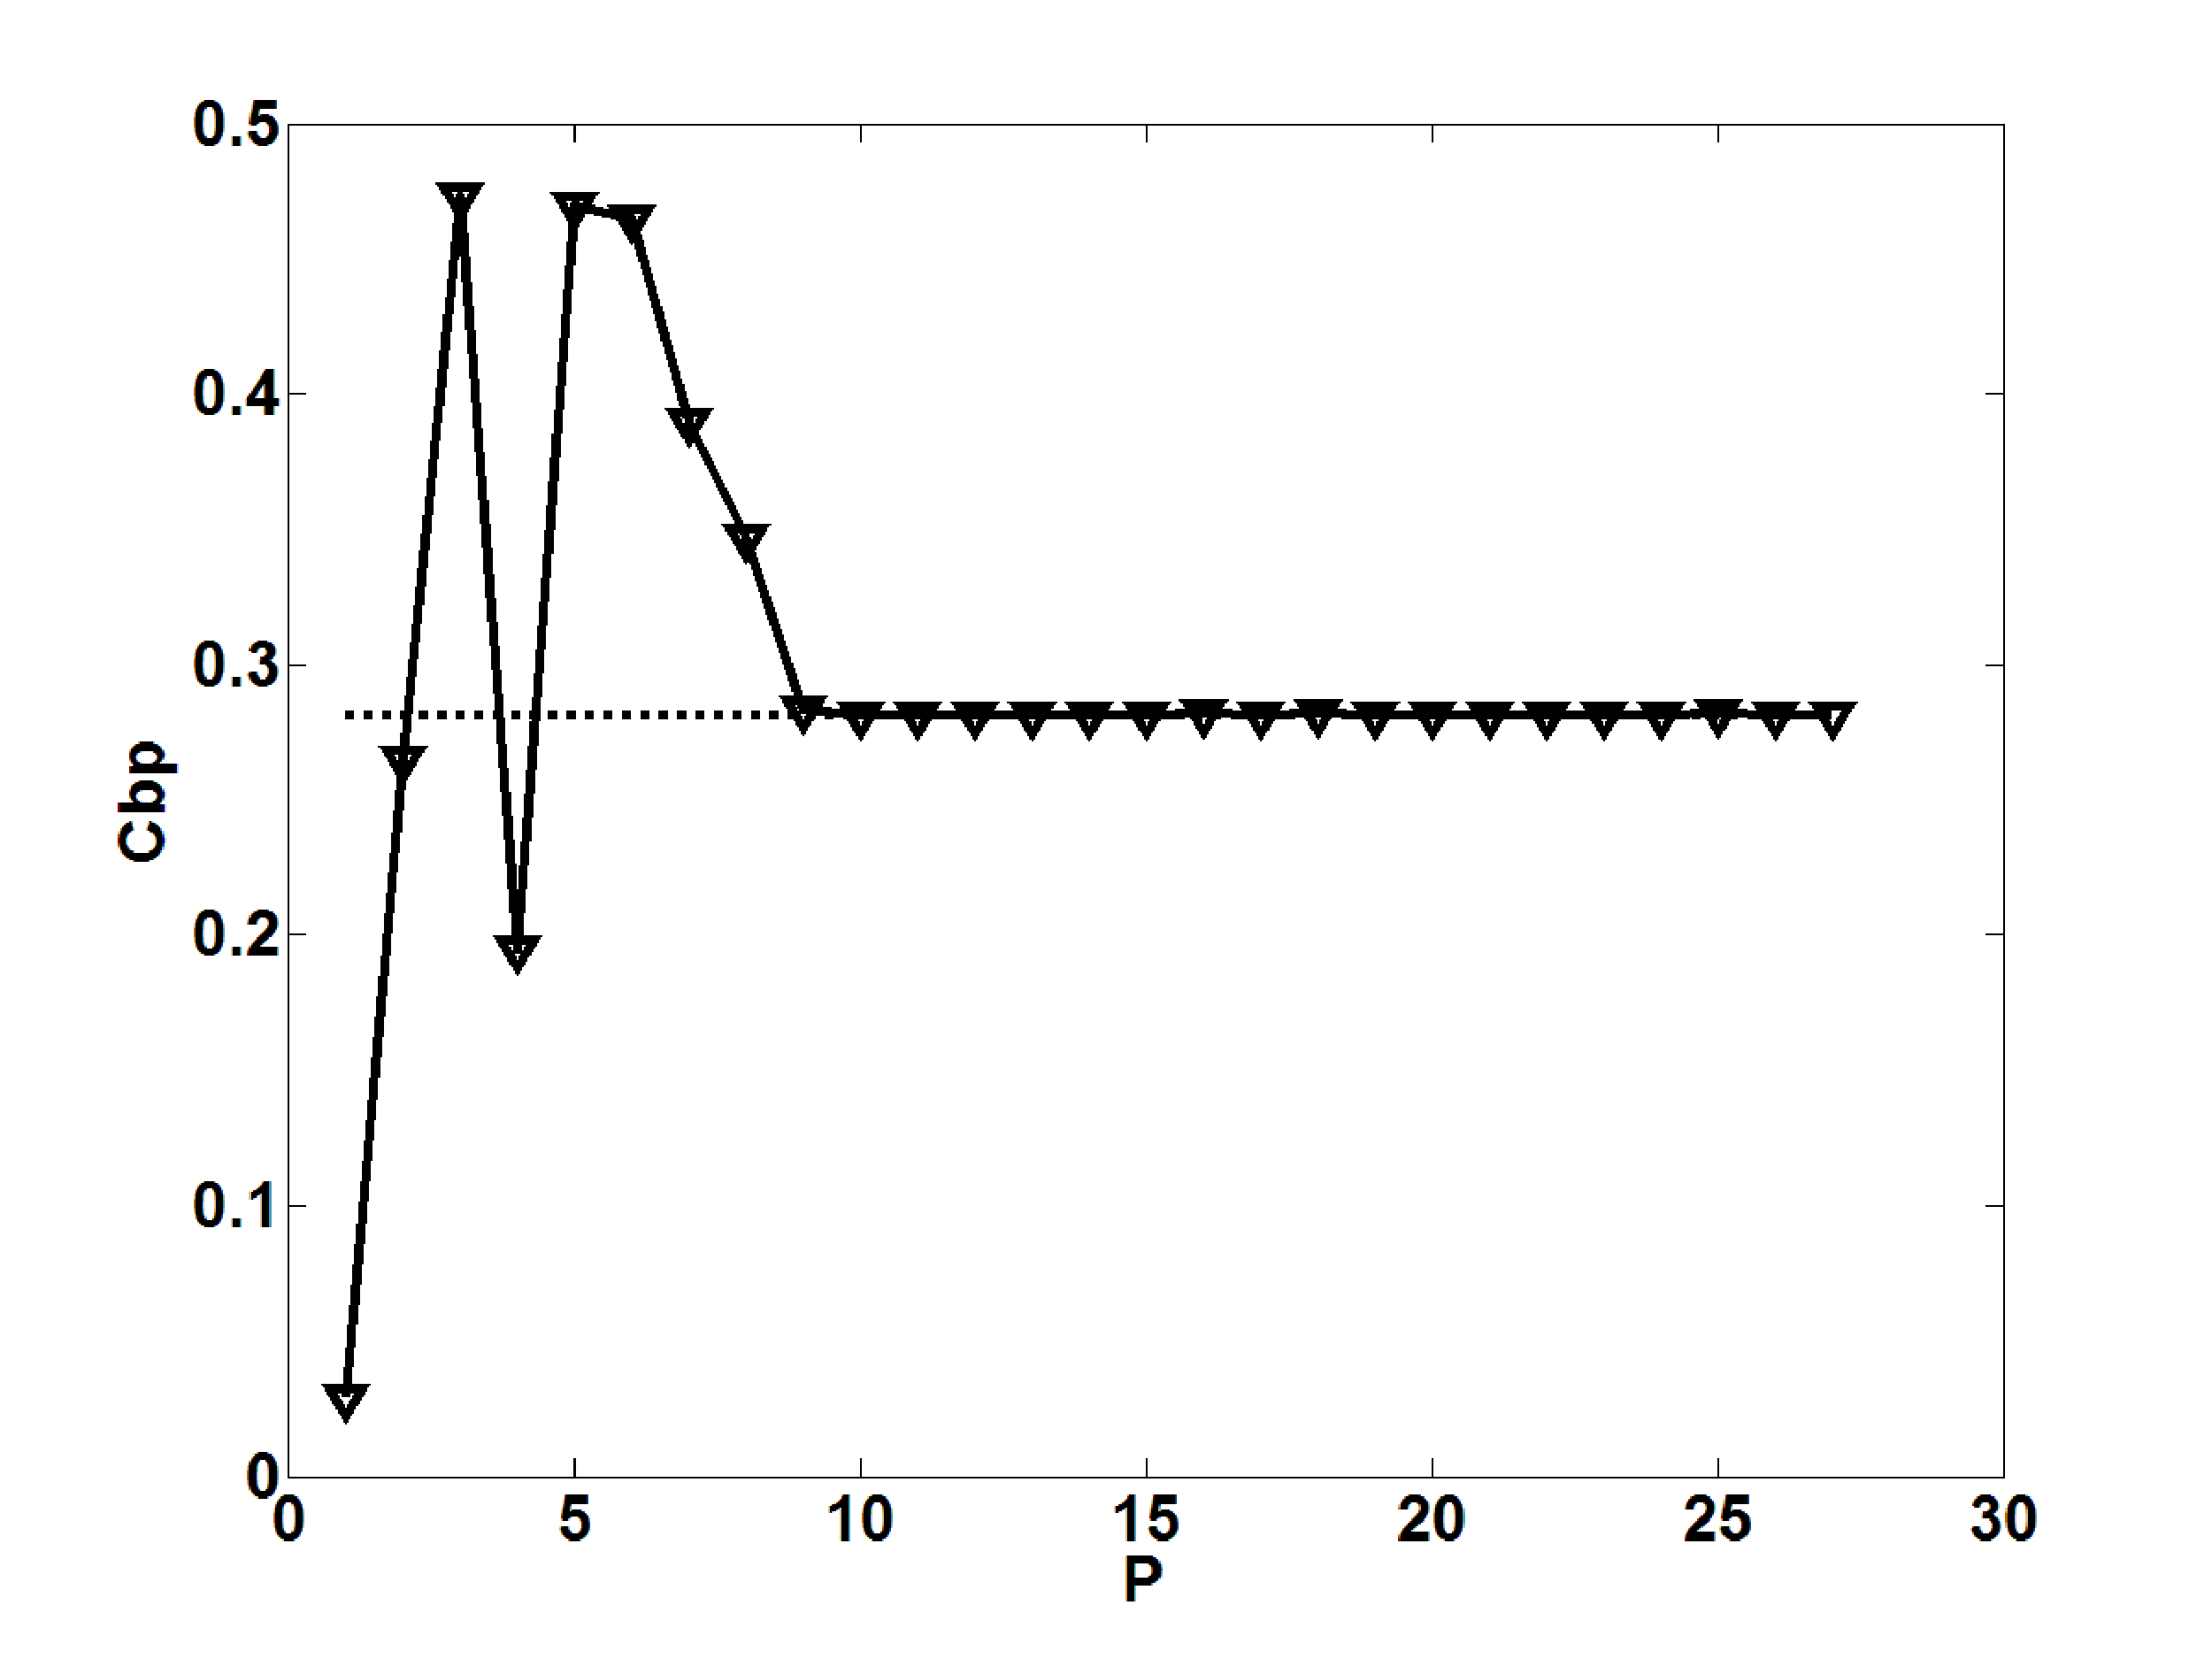
\includegraphics[width=0.3\textwidth]{Cbp_imparB10}
%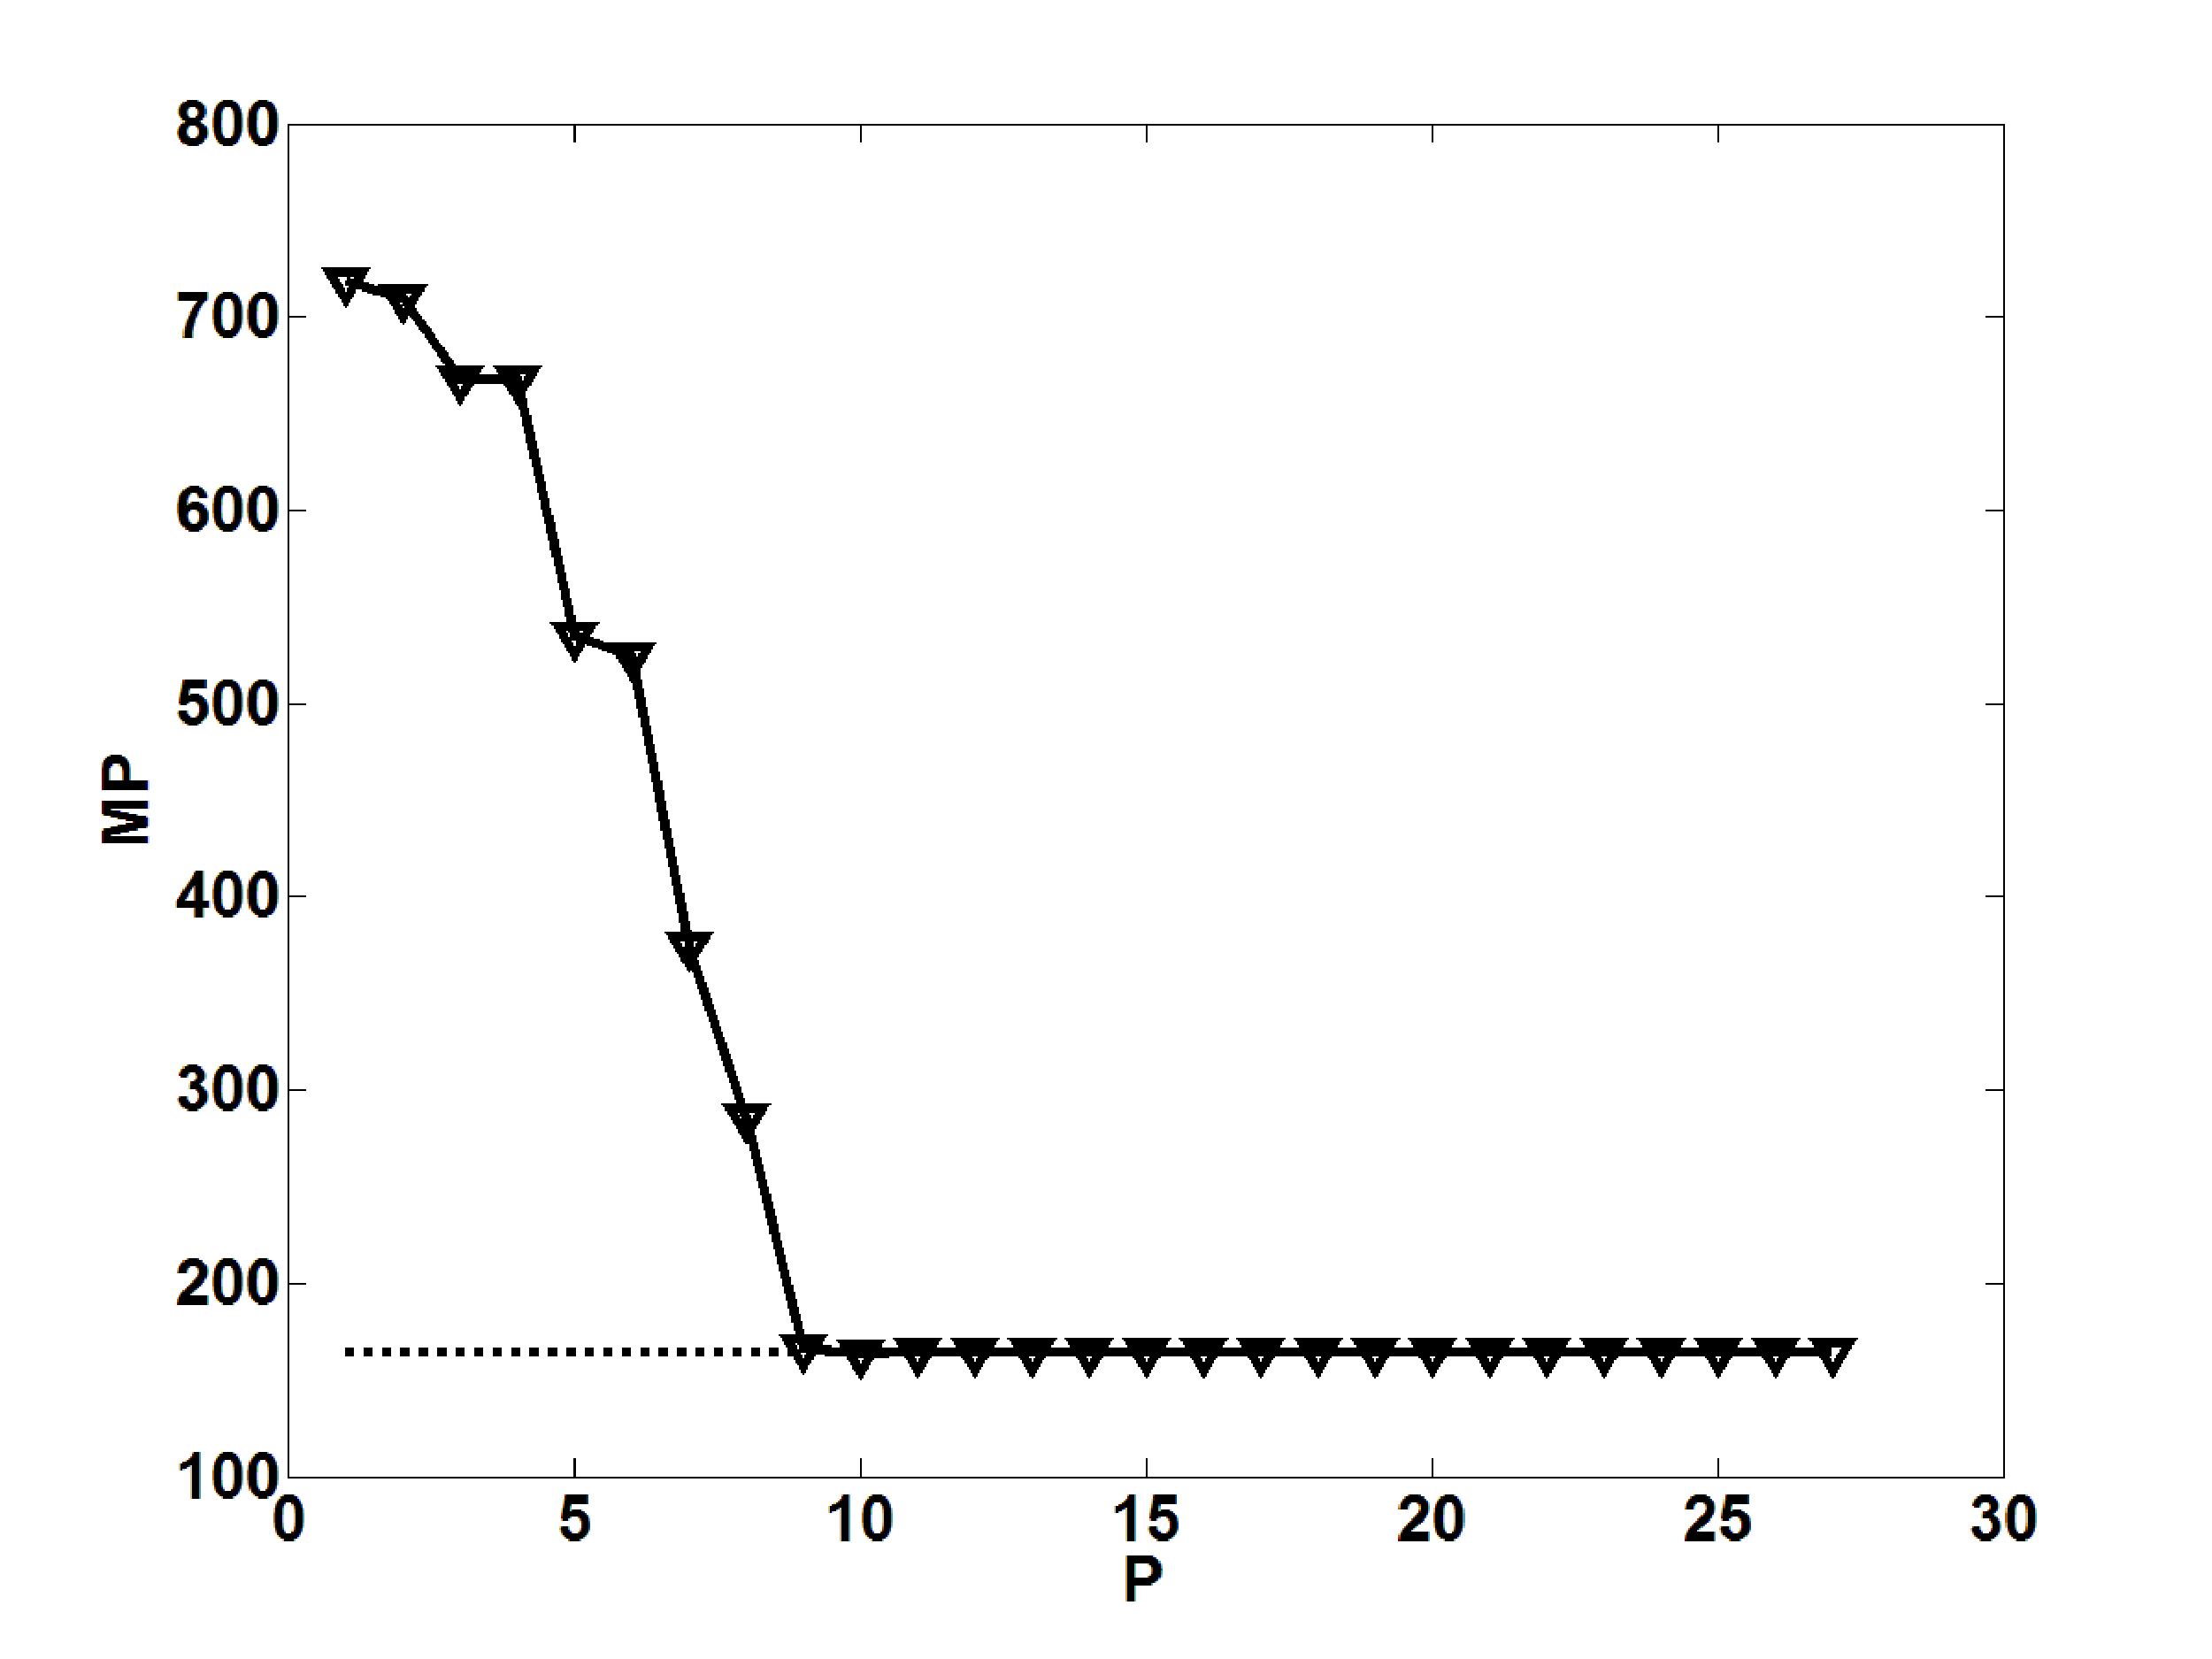
\includegraphics[width=0.3\textwidth]{Miss_imparB10}
%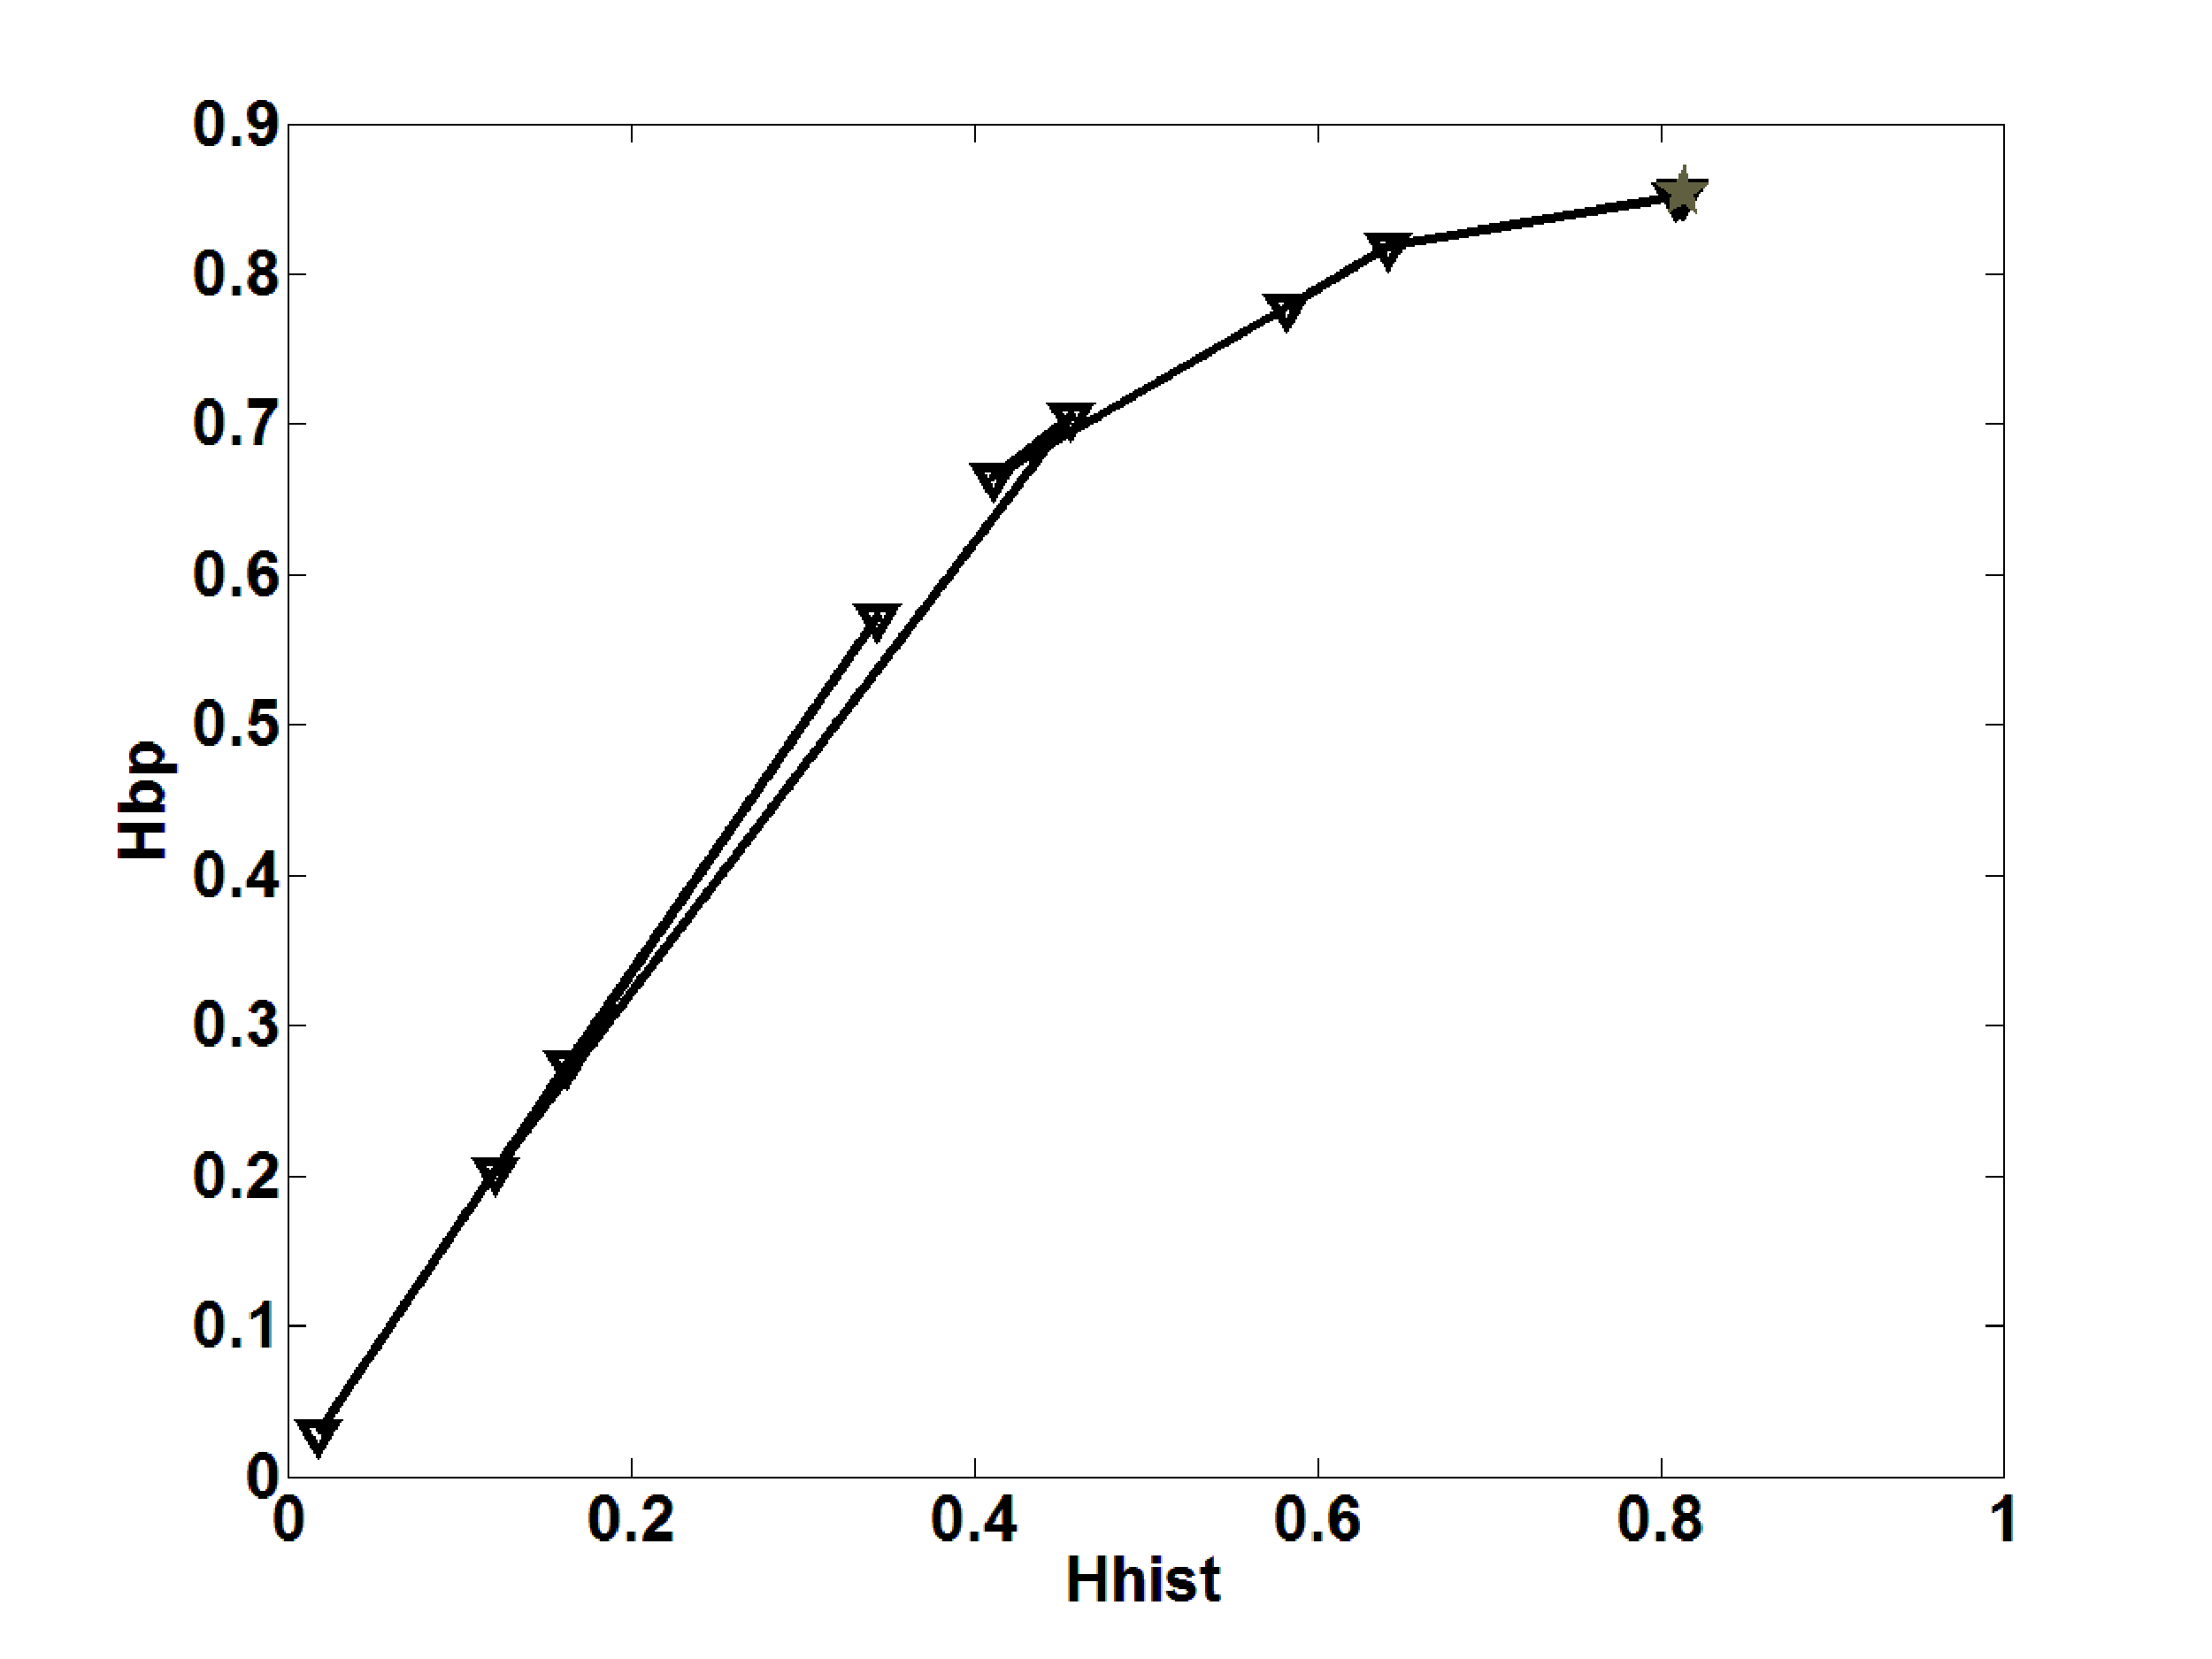
\includegraphics[width=0.3\textwidth]{HhistHbp_imparB10}
%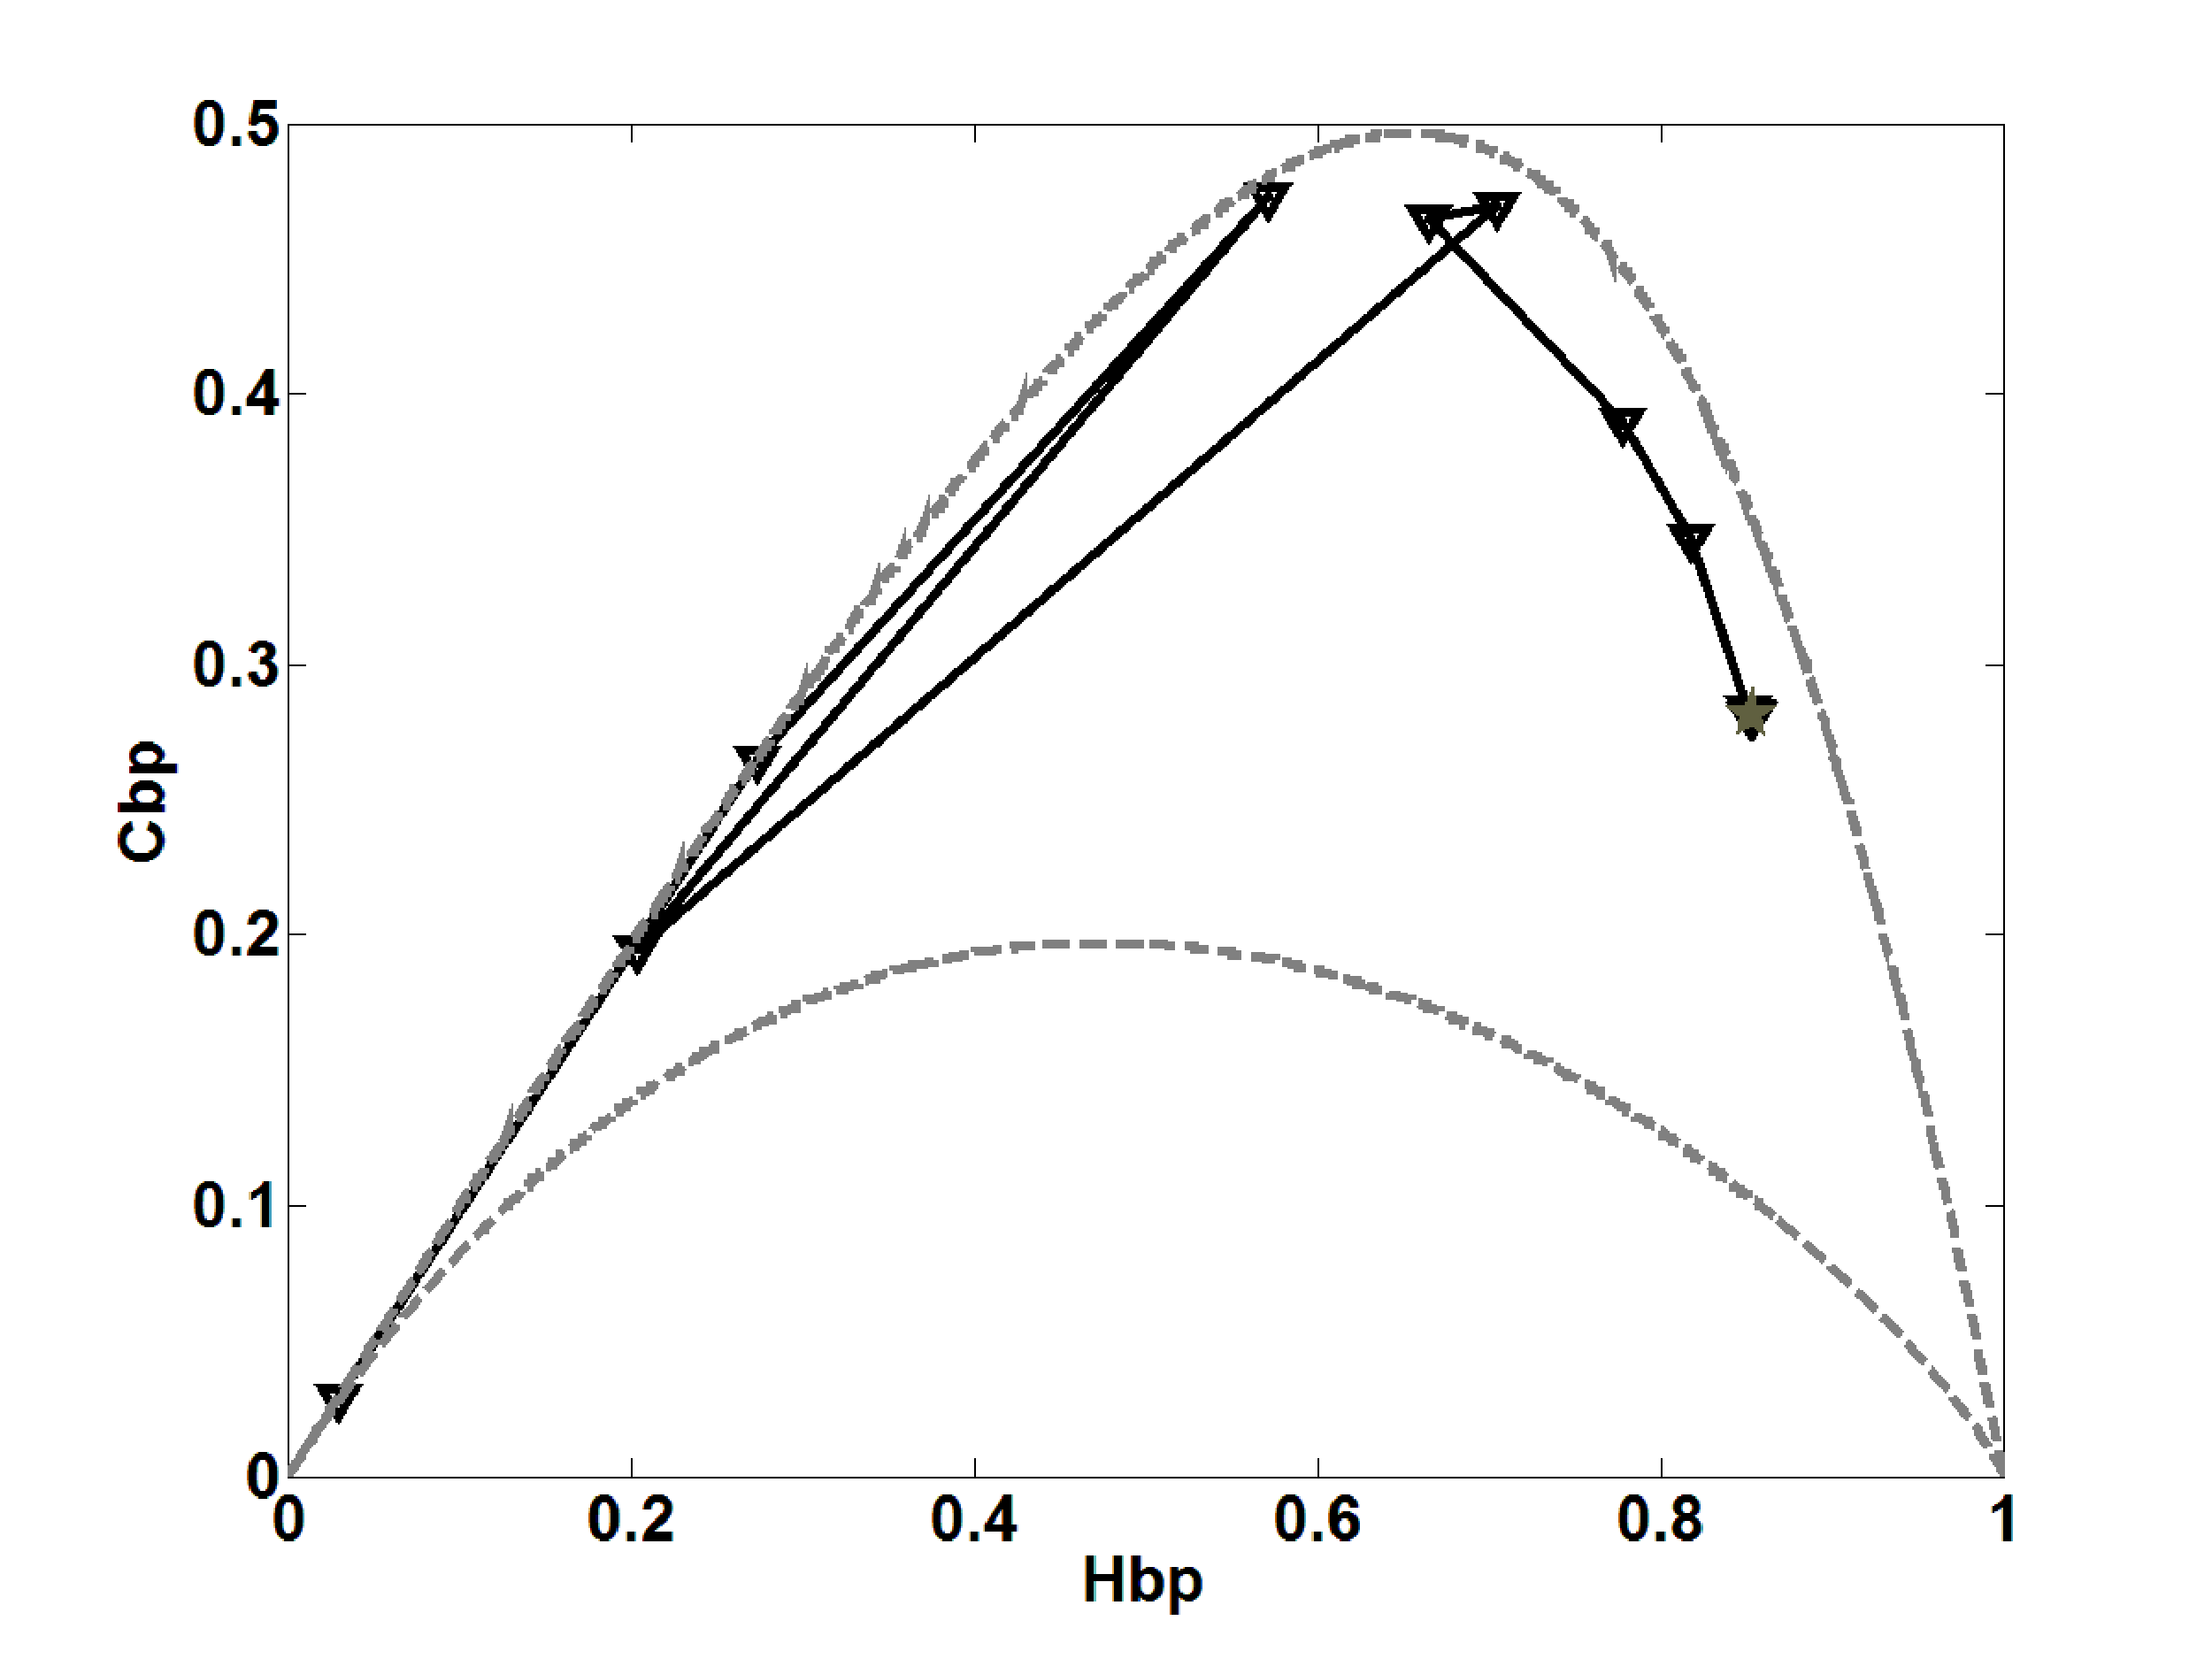
\includegraphics[width=0.3\textwidth]{HbpCbp_imparB10}
%\caption{Statistical properties of EVEN, obtained by skipping the values in the even positions of the time series of  SWITCH,  using decimal representation: (a) $H_{hist}$ vs $P$ (b) $H_{BP}$ vs $P$ (c) $C_{BP}$ vs $P$ (d) Number of missing ordering patterns $MP$ vs $P$. In Figures (a) to (d) dashed line correspond to floating point numbers. (e) representation in the $H_{hist},H_{BP}$ plane in the the decimal numerical system.  The star represents the state for floating points numbers. (f) representation in the $H_{BP},C_{BP}$ plane.  The star represents the state for floating points numbers. } \label{fig:seqimpardec}
%\end{figure}
%
%%%%%%%%%%%%%%%%%%%%%%%%%%%%%%%Fig 10.
%\begin{figure}
%\includegraphics[width=0.3\textwidth]{Hhist_imparB2}
%\includegraphics[width=0.3\textwidth]{Hbp_imparB2}
%\includegraphics[width=0.3\textwidth]{Cbp_imparB2}
%\includegraphics[width=0.3\textwidth]{Miss_imparB2}
%\includegraphics[width=0.3\textwidth]{HhistHbp_imparB2}
%\includegraphics[width=0.3\textwidth]{HbpCbp_imparB2}
%\caption{Statistical properties of EVEN, obtained by skipping the values in the odd position of the time series of  SWITCH,  using binary representation: (a) $H_{hist}$ vs $P$ (b) $H_{BP}$ vs $P$ (c) $C_{BP}$ vs $P$ (d) Number of missing ordering patterns $MP$ vs $P$. In Figures (a) to (d) dashed line correspond to floating point numbers. (e) representation in the $H_{hist},H_{BP}$ plane in the the binary numerical system.  The star represents the state for floating points numbers. (f) representation in the $H_{BP},C_{BP}$ plane.  The star represents the state for floating points numbers.  } \label{fig:seqimparbin}
%\end{figure}
%
%%%%%%%%%%%%%%%%%%%%%%%%%%%
%%%%%%%%%%%%%%%%%%%%%%%%%%% Fig.11
\center
\begin{figure}
\includegraphics[width=0.8\textwidth]{MeanPeriod_logisticoB10}
\caption{Period $T$ as a function of de number of decimal digits $P$ for the LOG map.} \label{fig:perio}
\end{figure}



